% Options for packages loaded elsewhere
\PassOptionsToPackage{unicode}{hyperref}
\PassOptionsToPackage{hyphens}{url}
%
\documentclass[
  landscape]{article}
\usepackage{amsmath,amssymb}
\usepackage{iftex}
\ifPDFTeX
  \usepackage[T1]{fontenc}
  \usepackage[utf8]{inputenc}
  \usepackage{textcomp} % provide euro and other symbols
\else % if luatex or xetex
  \usepackage{unicode-math} % this also loads fontspec
  \defaultfontfeatures{Scale=MatchLowercase}
  \defaultfontfeatures[\rmfamily]{Ligatures=TeX,Scale=1}
\fi
\usepackage{lmodern}
\ifPDFTeX\else
  % xetex/luatex font selection
\fi
% Use upquote if available, for straight quotes in verbatim environments
\IfFileExists{upquote.sty}{\usepackage{upquote}}{}
\IfFileExists{microtype.sty}{% use microtype if available
  \usepackage[]{microtype}
  \UseMicrotypeSet[protrusion]{basicmath} % disable protrusion for tt fonts
}{}
\makeatletter
\@ifundefined{KOMAClassName}{% if non-KOMA class
  \IfFileExists{parskip.sty}{%
    \usepackage{parskip}
  }{% else
    \setlength{\parindent}{0pt}
    \setlength{\parskip}{6pt plus 2pt minus 1pt}}
}{% if KOMA class
  \KOMAoptions{parskip=half}}
\makeatother
\usepackage{xcolor}
\usepackage[margin=1in]{geometry}
\usepackage{longtable,booktabs,array}
\usepackage{calc} % for calculating minipage widths
% Correct order of tables after \paragraph or \subparagraph
\usepackage{etoolbox}
\makeatletter
\patchcmd\longtable{\par}{\if@noskipsec\mbox{}\fi\par}{}{}
\makeatother
% Allow footnotes in longtable head/foot
\IfFileExists{footnotehyper.sty}{\usepackage{footnotehyper}}{\usepackage{footnote}}
\makesavenoteenv{longtable}
\usepackage{graphicx}
\makeatletter
\def\maxwidth{\ifdim\Gin@nat@width>\linewidth\linewidth\else\Gin@nat@width\fi}
\def\maxheight{\ifdim\Gin@nat@height>\textheight\textheight\else\Gin@nat@height\fi}
\makeatother
% Scale images if necessary, so that they will not overflow the page
% margins by default, and it is still possible to overwrite the defaults
% using explicit options in \includegraphics[width, height, ...]{}
\setkeys{Gin}{width=\maxwidth,height=\maxheight,keepaspectratio}
% Set default figure placement to htbp
\makeatletter
\def\fps@figure{htbp}
\makeatother
\setlength{\emergencystretch}{3em} % prevent overfull lines
\providecommand{\tightlist}{%
  \setlength{\itemsep}{0pt}\setlength{\parskip}{0pt}}
\setcounter{secnumdepth}{5}
\usepackage{graphicx}
\usepackage{float}
\floatplacement{figure}{H}
\ifLuaTeX
  \usepackage{selnolig}  % disable illegal ligatures
\fi
\IfFileExists{bookmark.sty}{\usepackage{bookmark}}{\usepackage{hyperref}}
\IfFileExists{xurl.sty}{\usepackage{xurl}}{} % add URL line breaks if available
\urlstyle{same}
\hypersetup{
  pdftitle={Washington Crime Analysis Project},
  pdfauthor={Tyler Hart},
  hidelinks,
  pdfcreator={LaTeX via pandoc}}

\title{Washington Crime Analysis Project}
\author{Tyler Hart}
\date{2024-01-23}

\begin{document}
\maketitle

{
\setcounter{tocdepth}{2}
\tableofcontents
}
\hypertarget{introduction}{%
\section{Introduction}\label{introduction}}

Three large cities in Washington - Bellevue, Spokane, and Tacoma - make
regular crime reports available. Spokane releases its data on a weekly
basis. This project collects and parses that data, and provides
up-to-date analysis. The same data is formatted and submitted annually
to the FBI NIBRS program as well. A lot of work is required to prepare
the data for submission to NIBRS, but it's more granular and includes
detailed information that weekly reports lack. Unfortunately, it takes a
year or more for current data to be available in the NIBRS portal. It
will most likely be late-2022 or early-2023 before 2021's data is ready.
We use the weekly reports to identify trends happening now and provide
up-to-date analysis. NIBRS-based analysis is a separate project. The
additional detail from years past informs our weekly analysis and helps
us frame questions better.

When this project began it was strictly focused on crime in Spokane.
It's since expanded to include other cities with similar population size
that also make crime data available regularly. Here are the three
covered cities and their population based on Census Bureau estimates for
2020:

\begin{longtable}[]{@{}rr@{}}
\toprule\noalign{}
City & Estimated 2020 Population \\
\midrule\noalign{}
\endhead
\bottomrule\noalign{}
\endlastfoot
Spokane & 222,050 \\
Tacoma & 219,995 \\
Bellevue & 148,073 \\
\end{longtable}

I'd have liked to include the city of Vancouver, as it has a population
between Bellevue and Tacoma, but they don't make regular crime data
reports available. Seattle is so much larger than all the other cities
that I've excluded its crime analysis from this project.

\hypertarget{incidents-over-time}{%
\section{Incidents Over Time}\label{incidents-over-time}}

We visualize incidents over time by totaling up incidents and plotting
them daily. Blue and red lines show average values using generalized
additive model (GAM) and linear model (LM), respectively. Then we break
down data for time series analysis and identify seasonality and trends.

\hypertarget{spokane}{%
\subsection{Spokane}\label{spokane}}

\begin{center}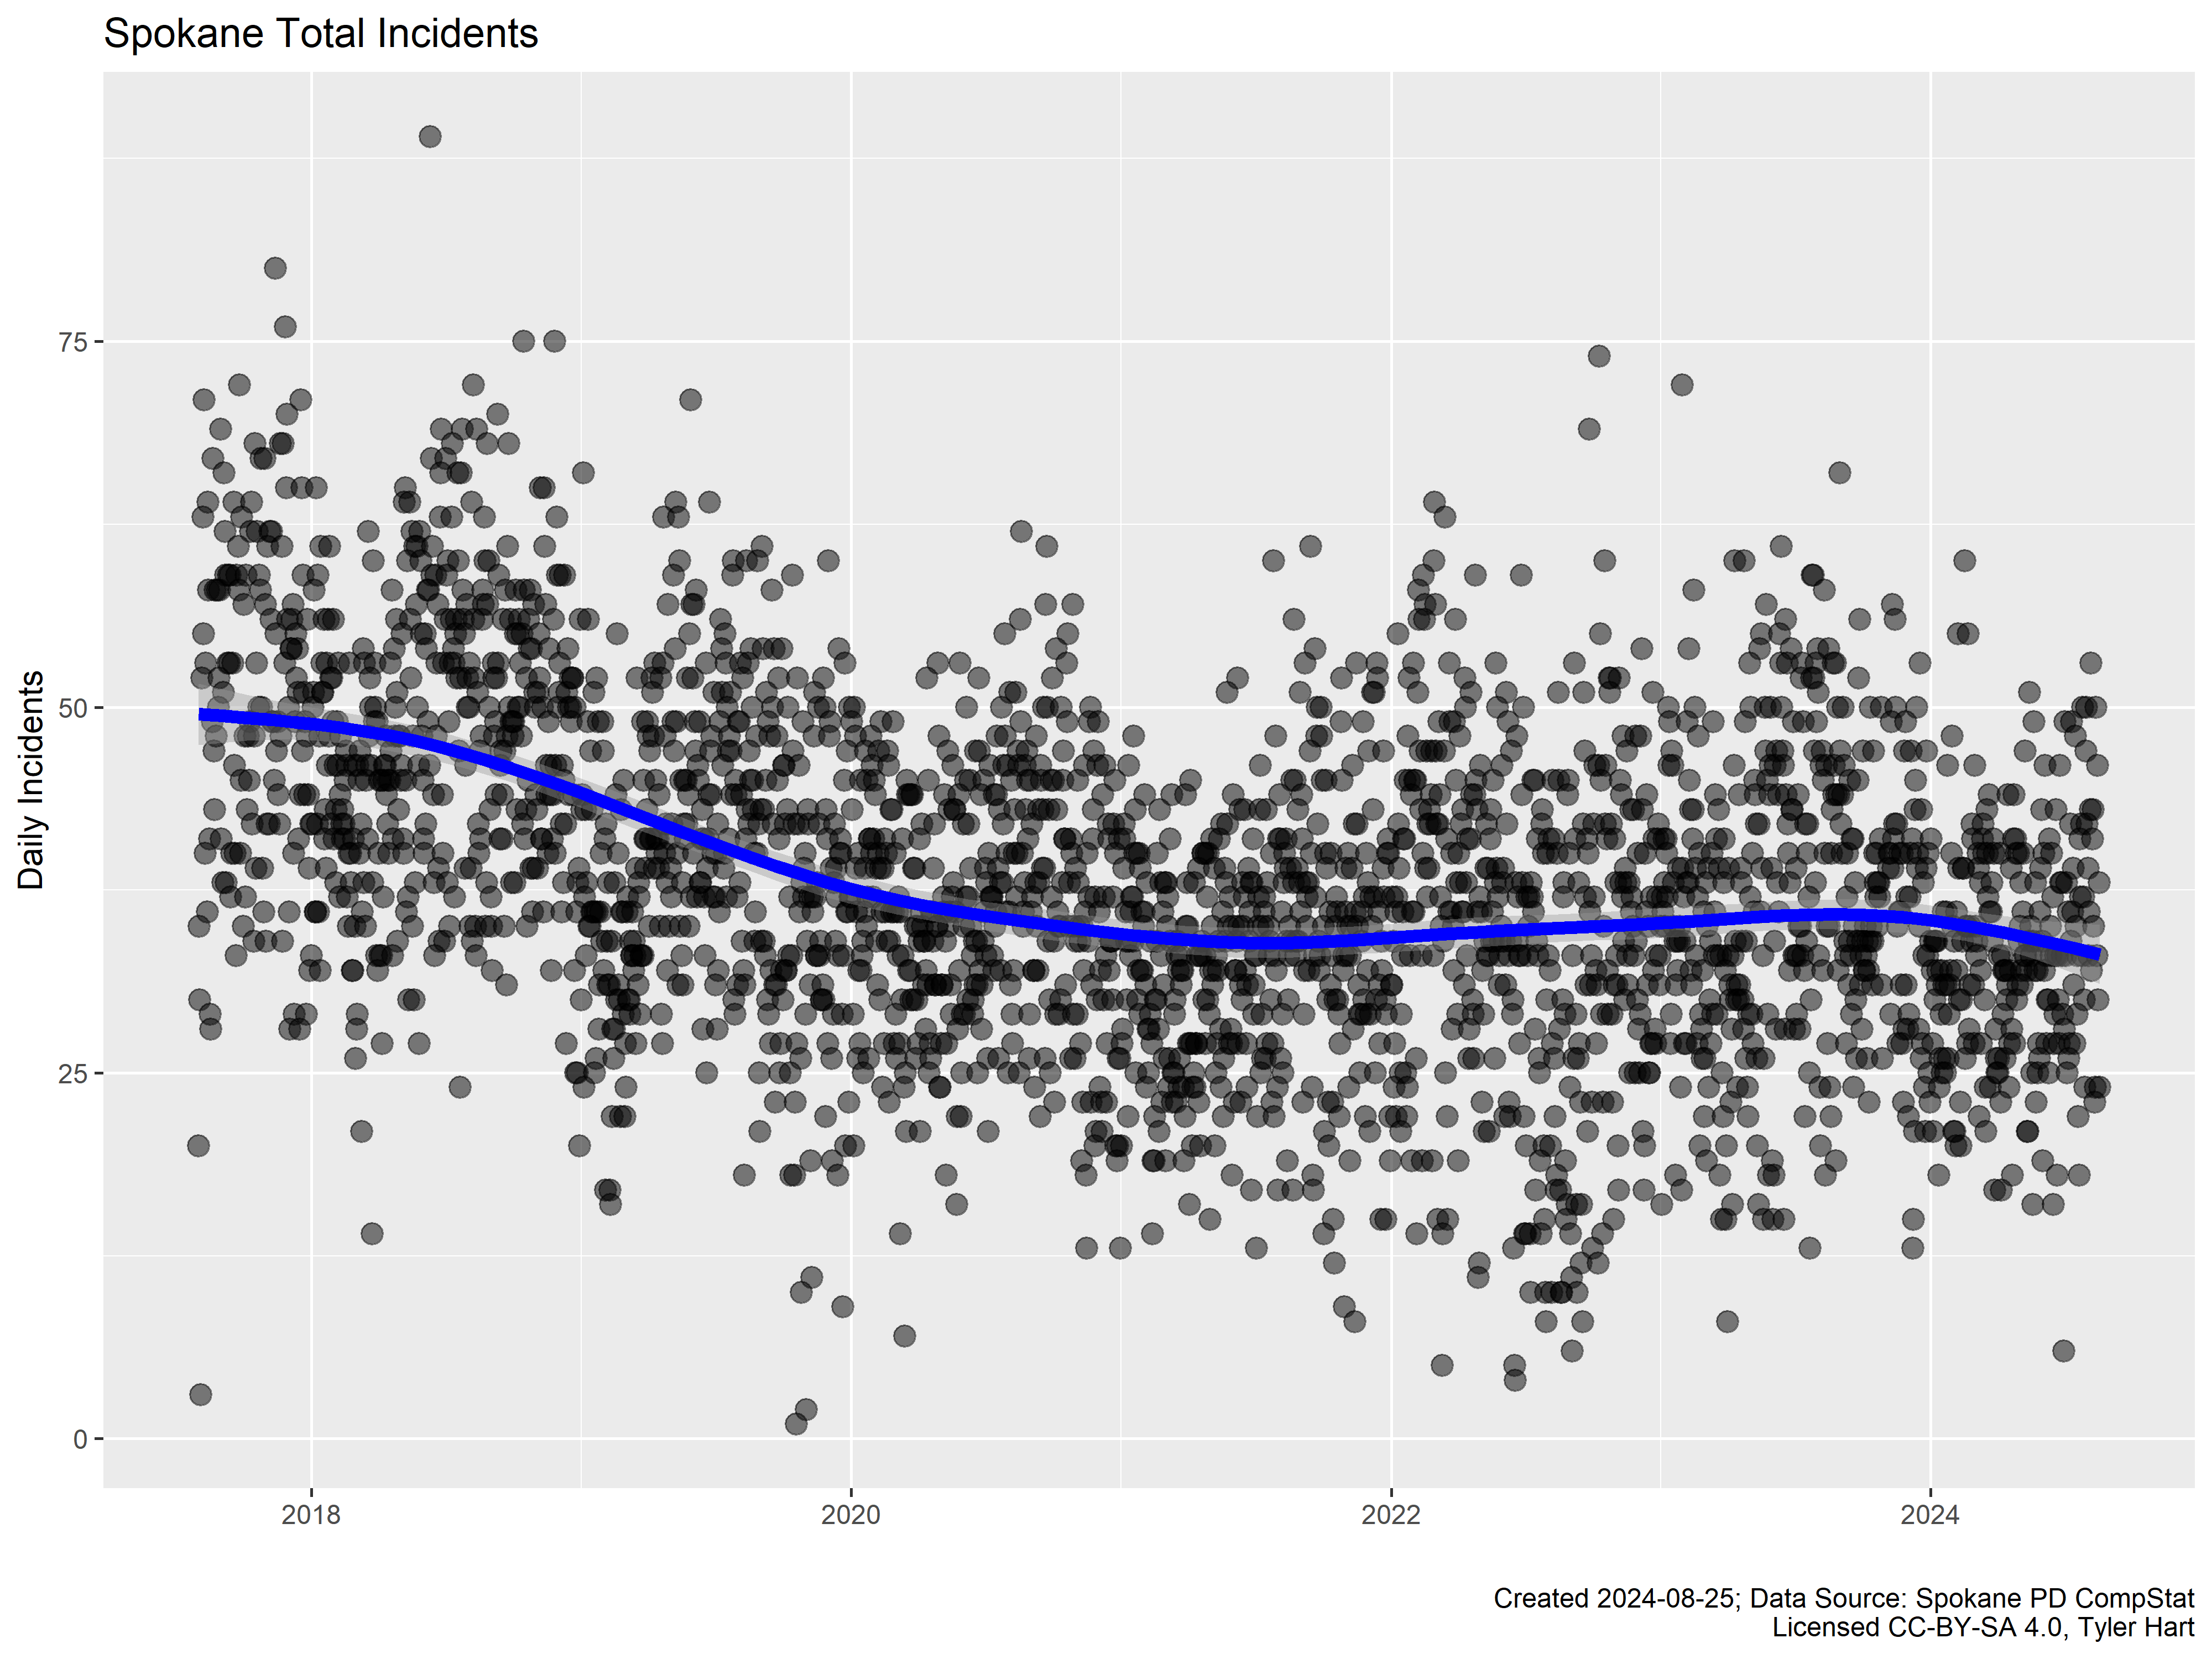
\includegraphics[width=\textwidth]{./figures/plot.offenses_over_time-1} \end{center}

\hypertarget{tacoma}{%
\subsection{Tacoma}\label{tacoma}}

\hypertarget{bellevue}{%
\subsection{Bellevue}\label{bellevue}}

\begin{center}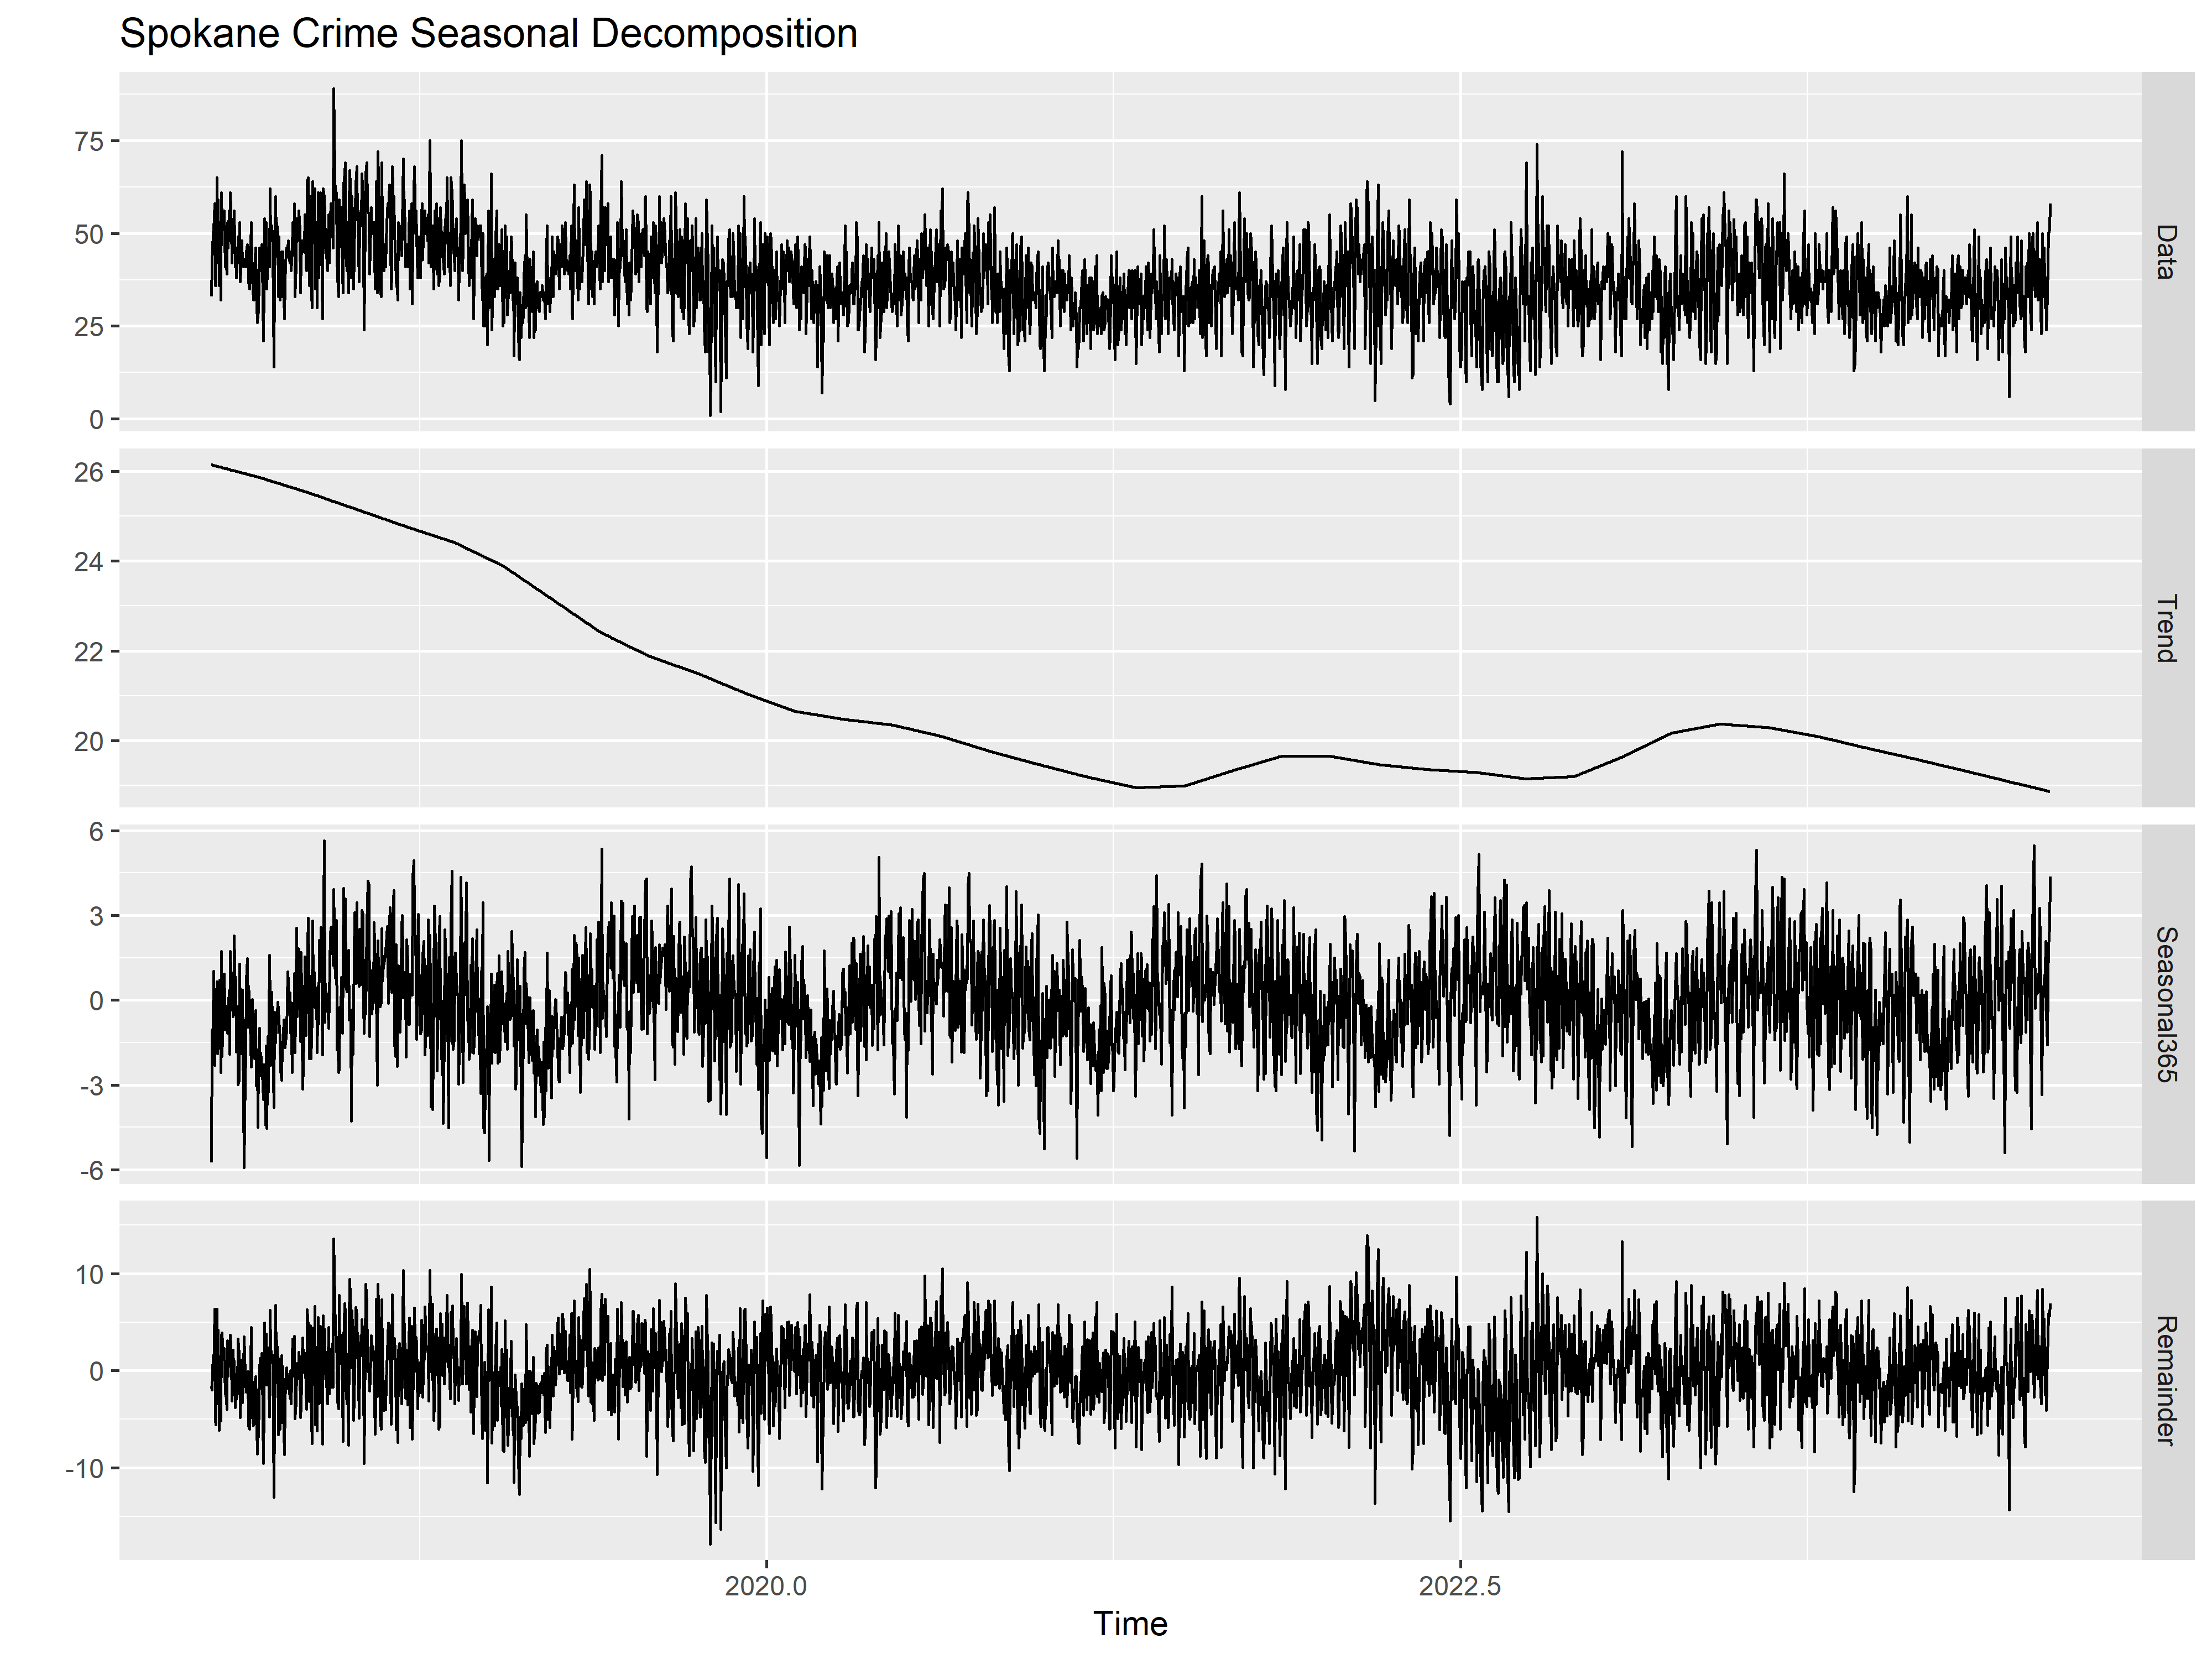
\includegraphics[width=\textwidth]{./figures/plot.crime_time_series_decomposition-1} \end{center}

\begin{center}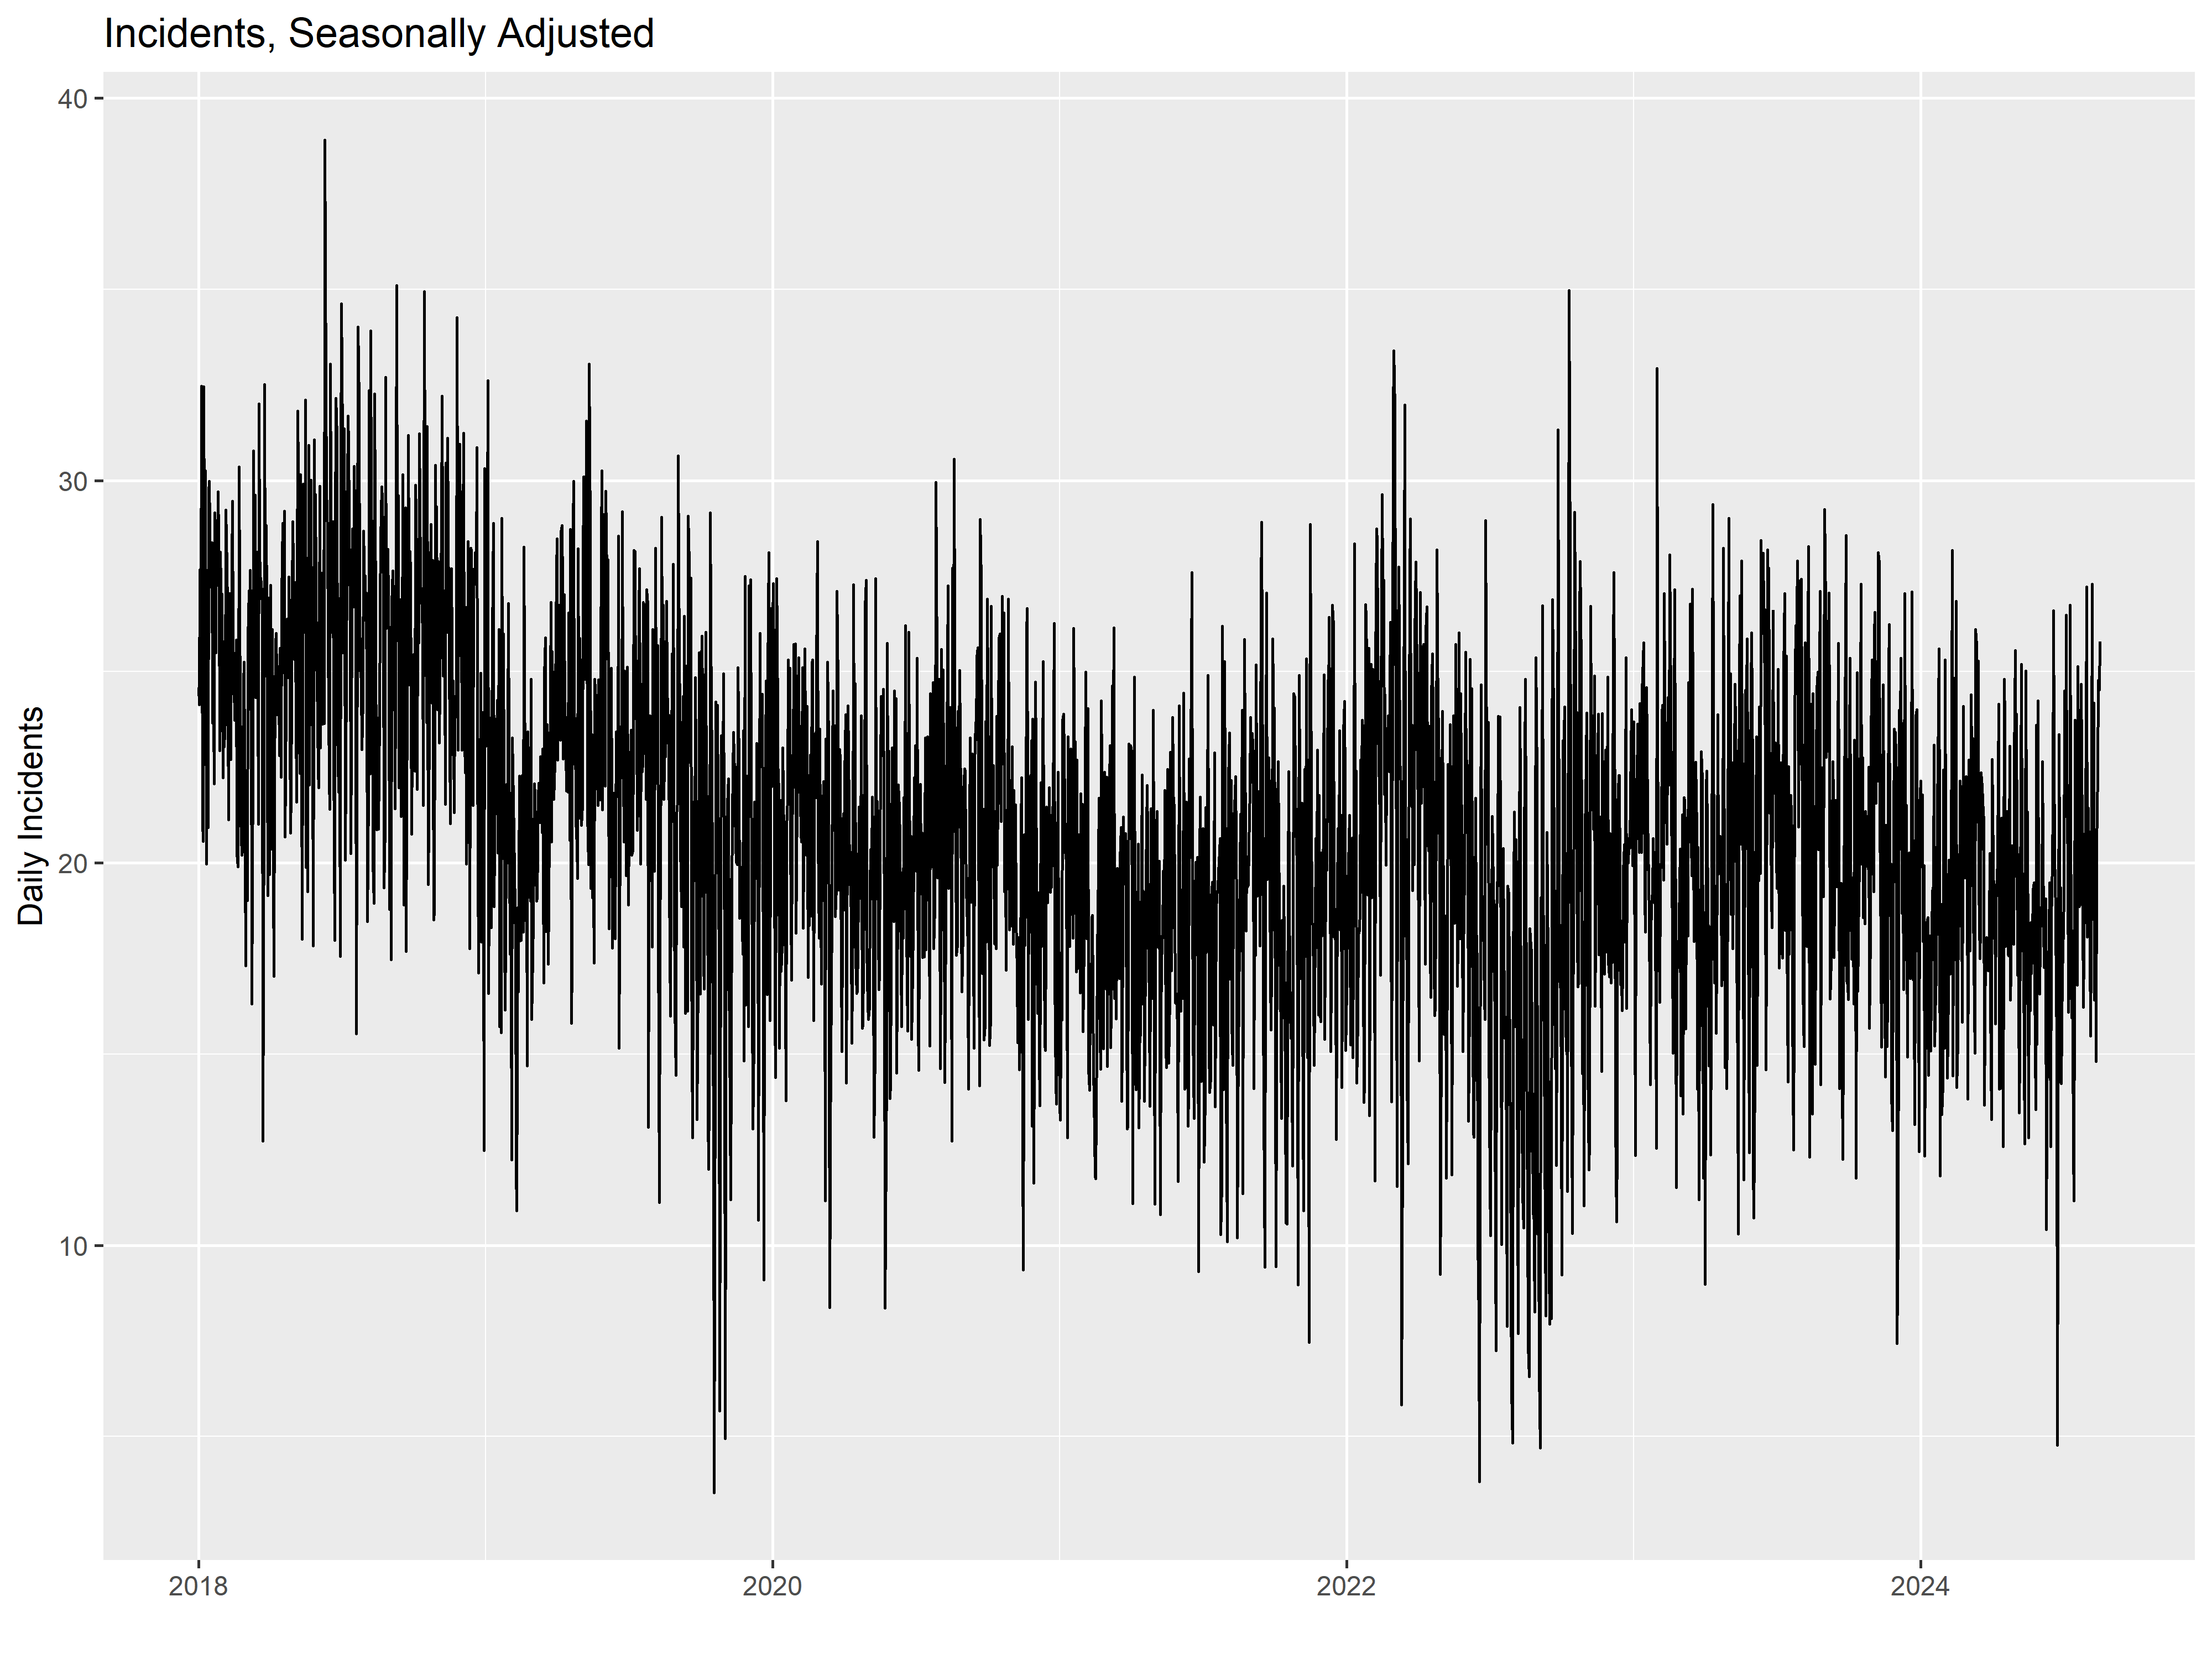
\includegraphics[width=\textwidth]{./figures/plot.crime_seasonally_adjusted-1} \end{center}

\begin{center}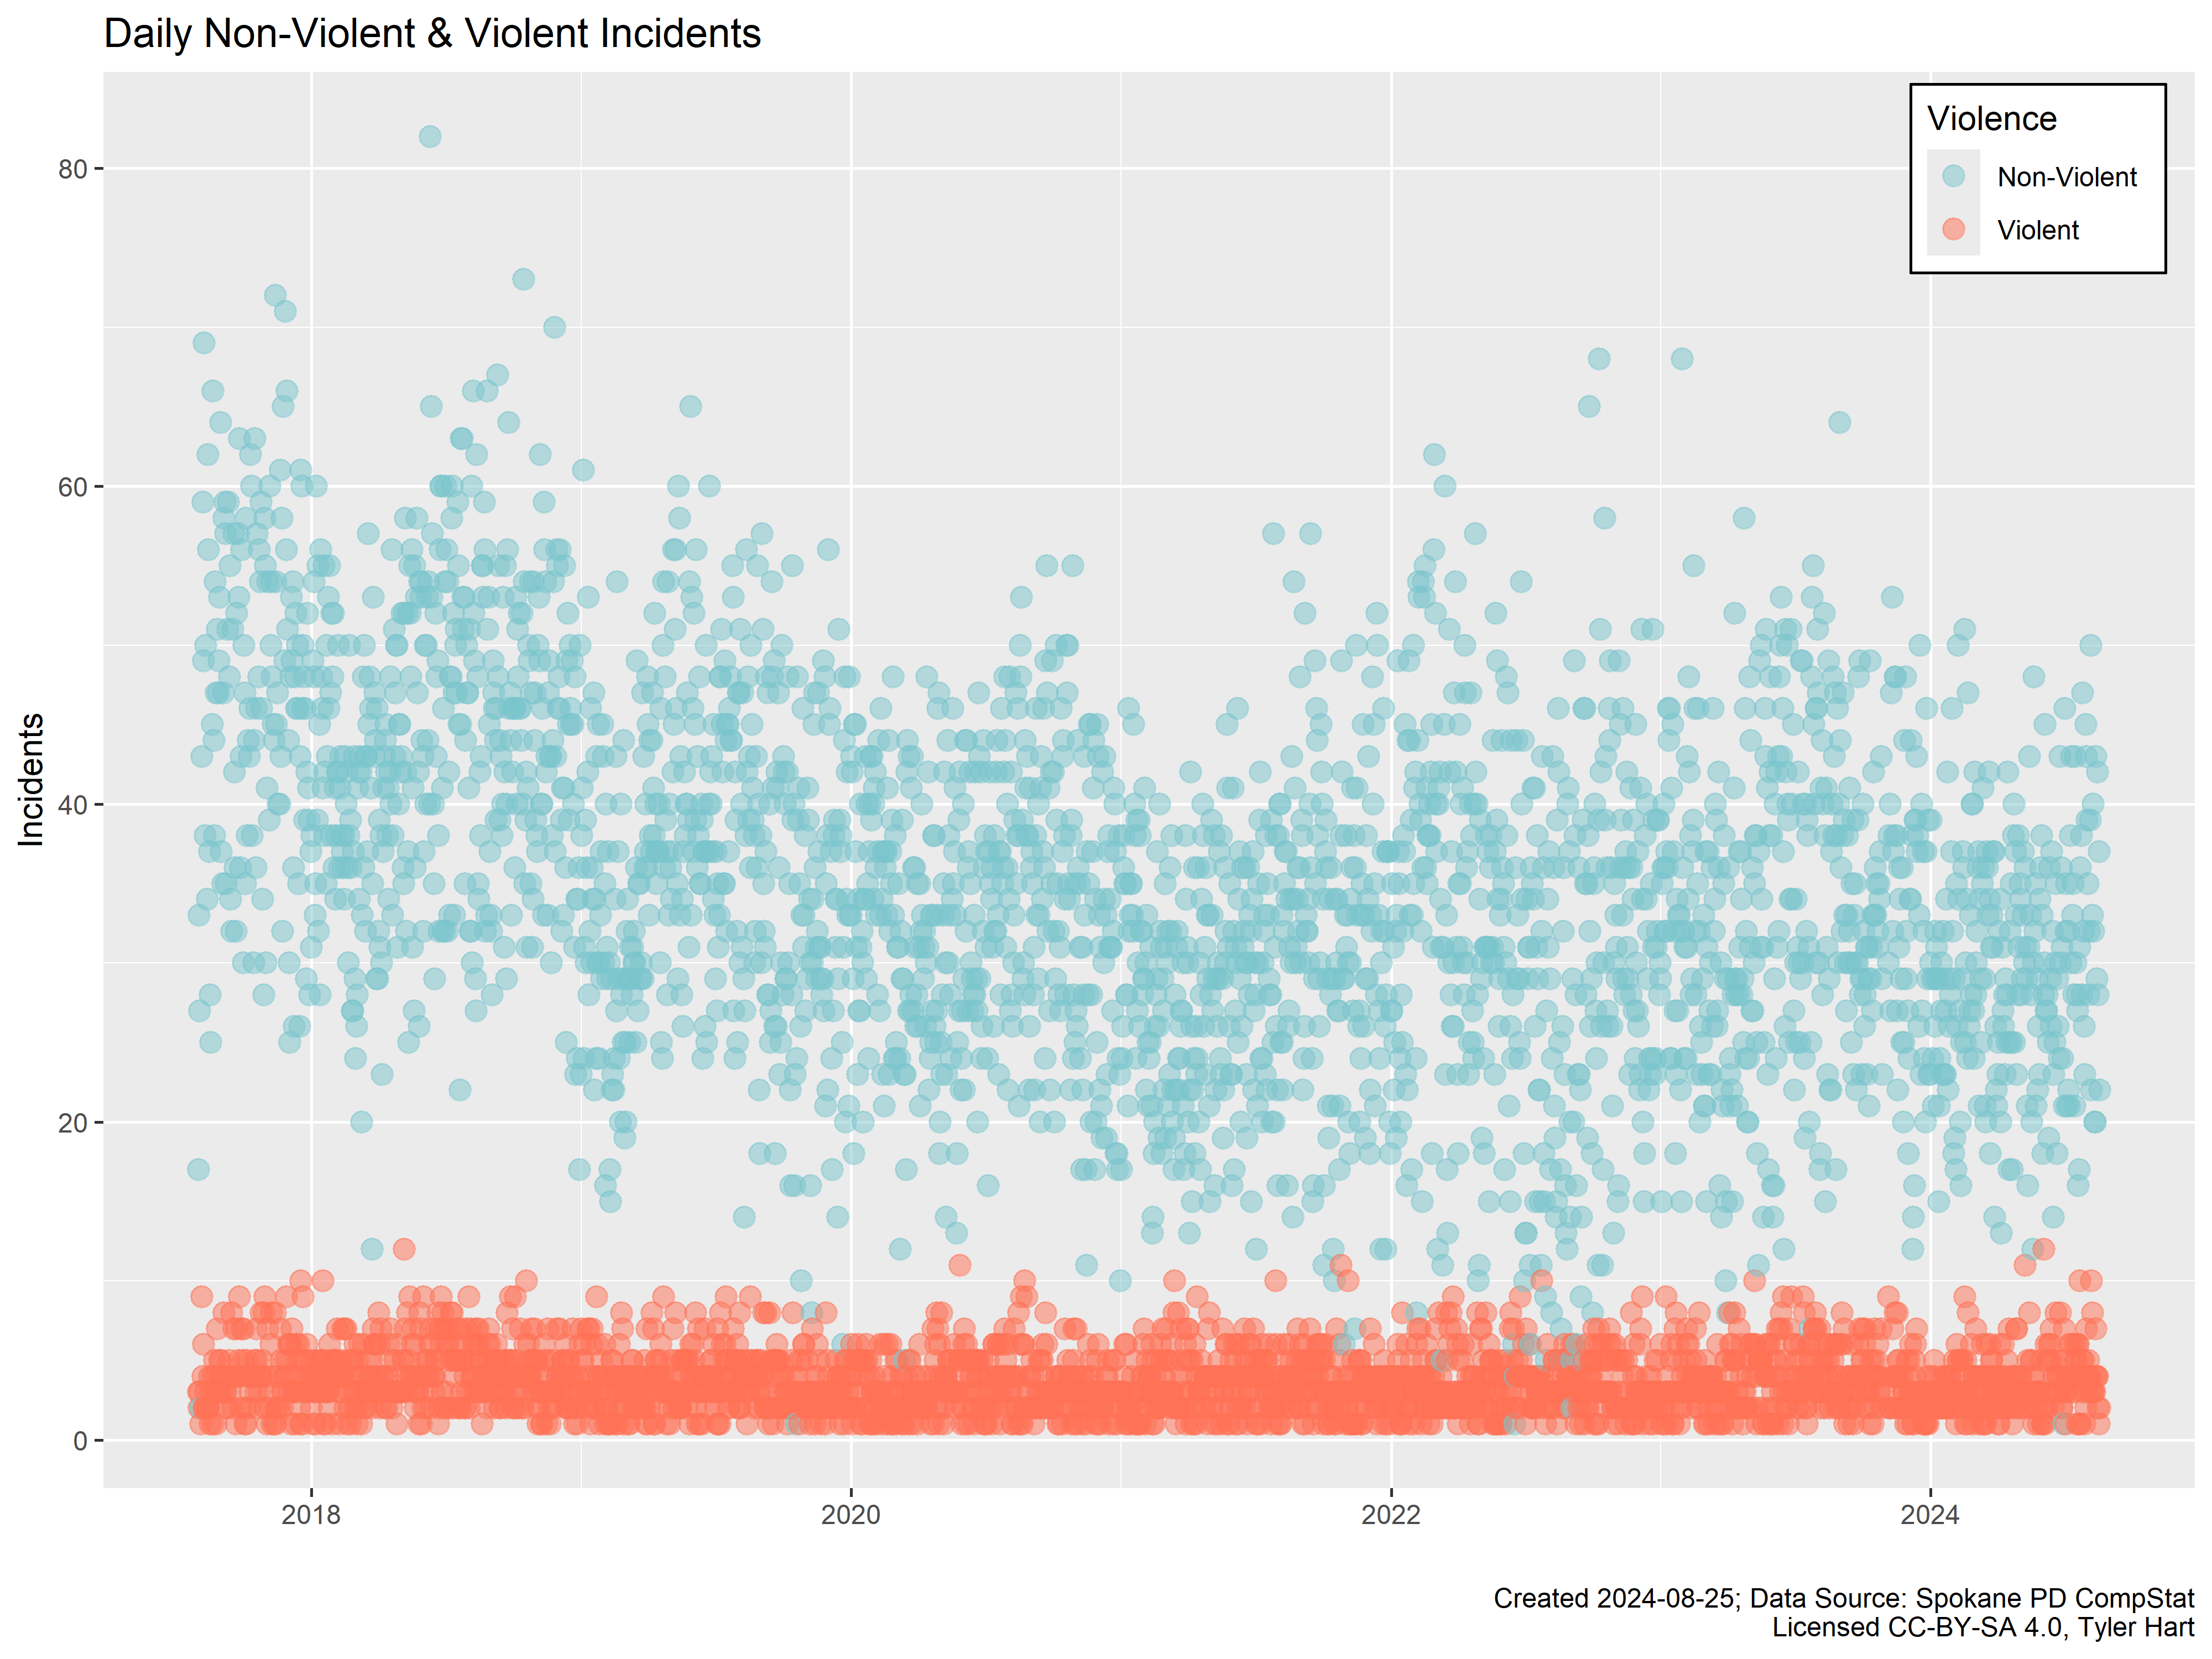
\includegraphics[width=\textwidth]{./figures/plot.offenses_over_time_violence-1} \end{center}

\begin{center}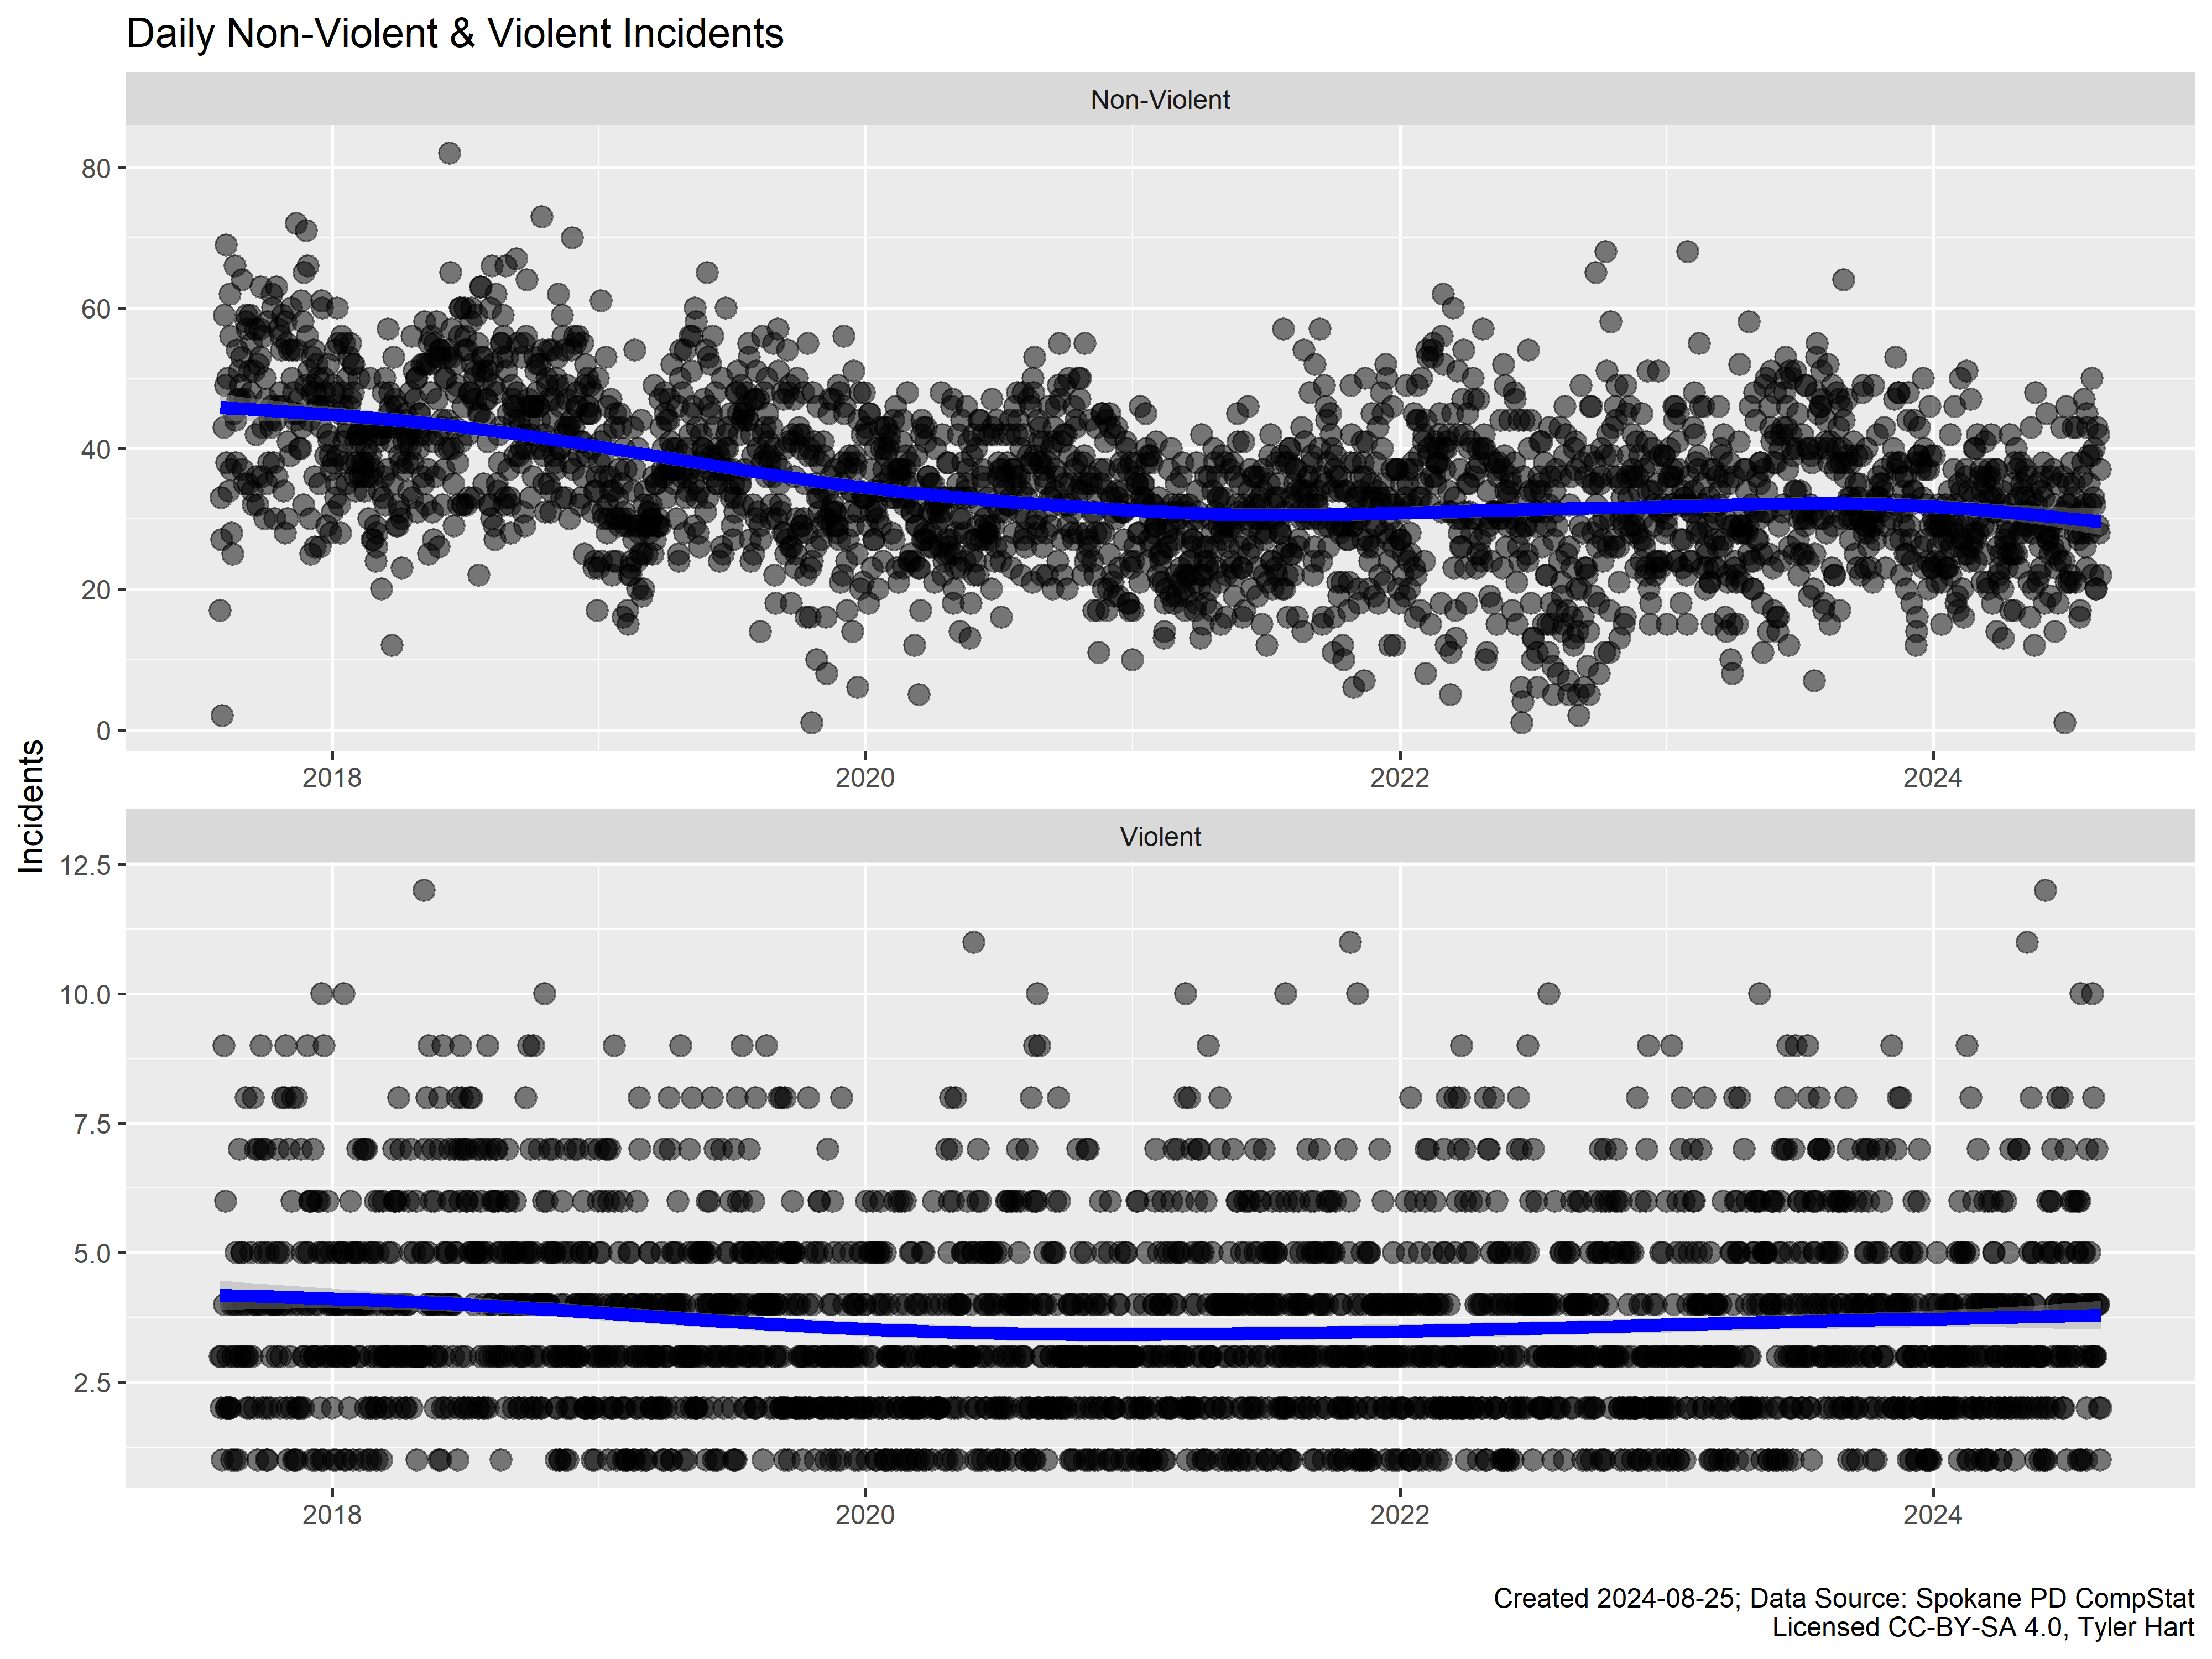
\includegraphics[width=\textwidth]{./figures/plot.offenses_over_time_violence_wrap-1} \end{center}

\begin{center}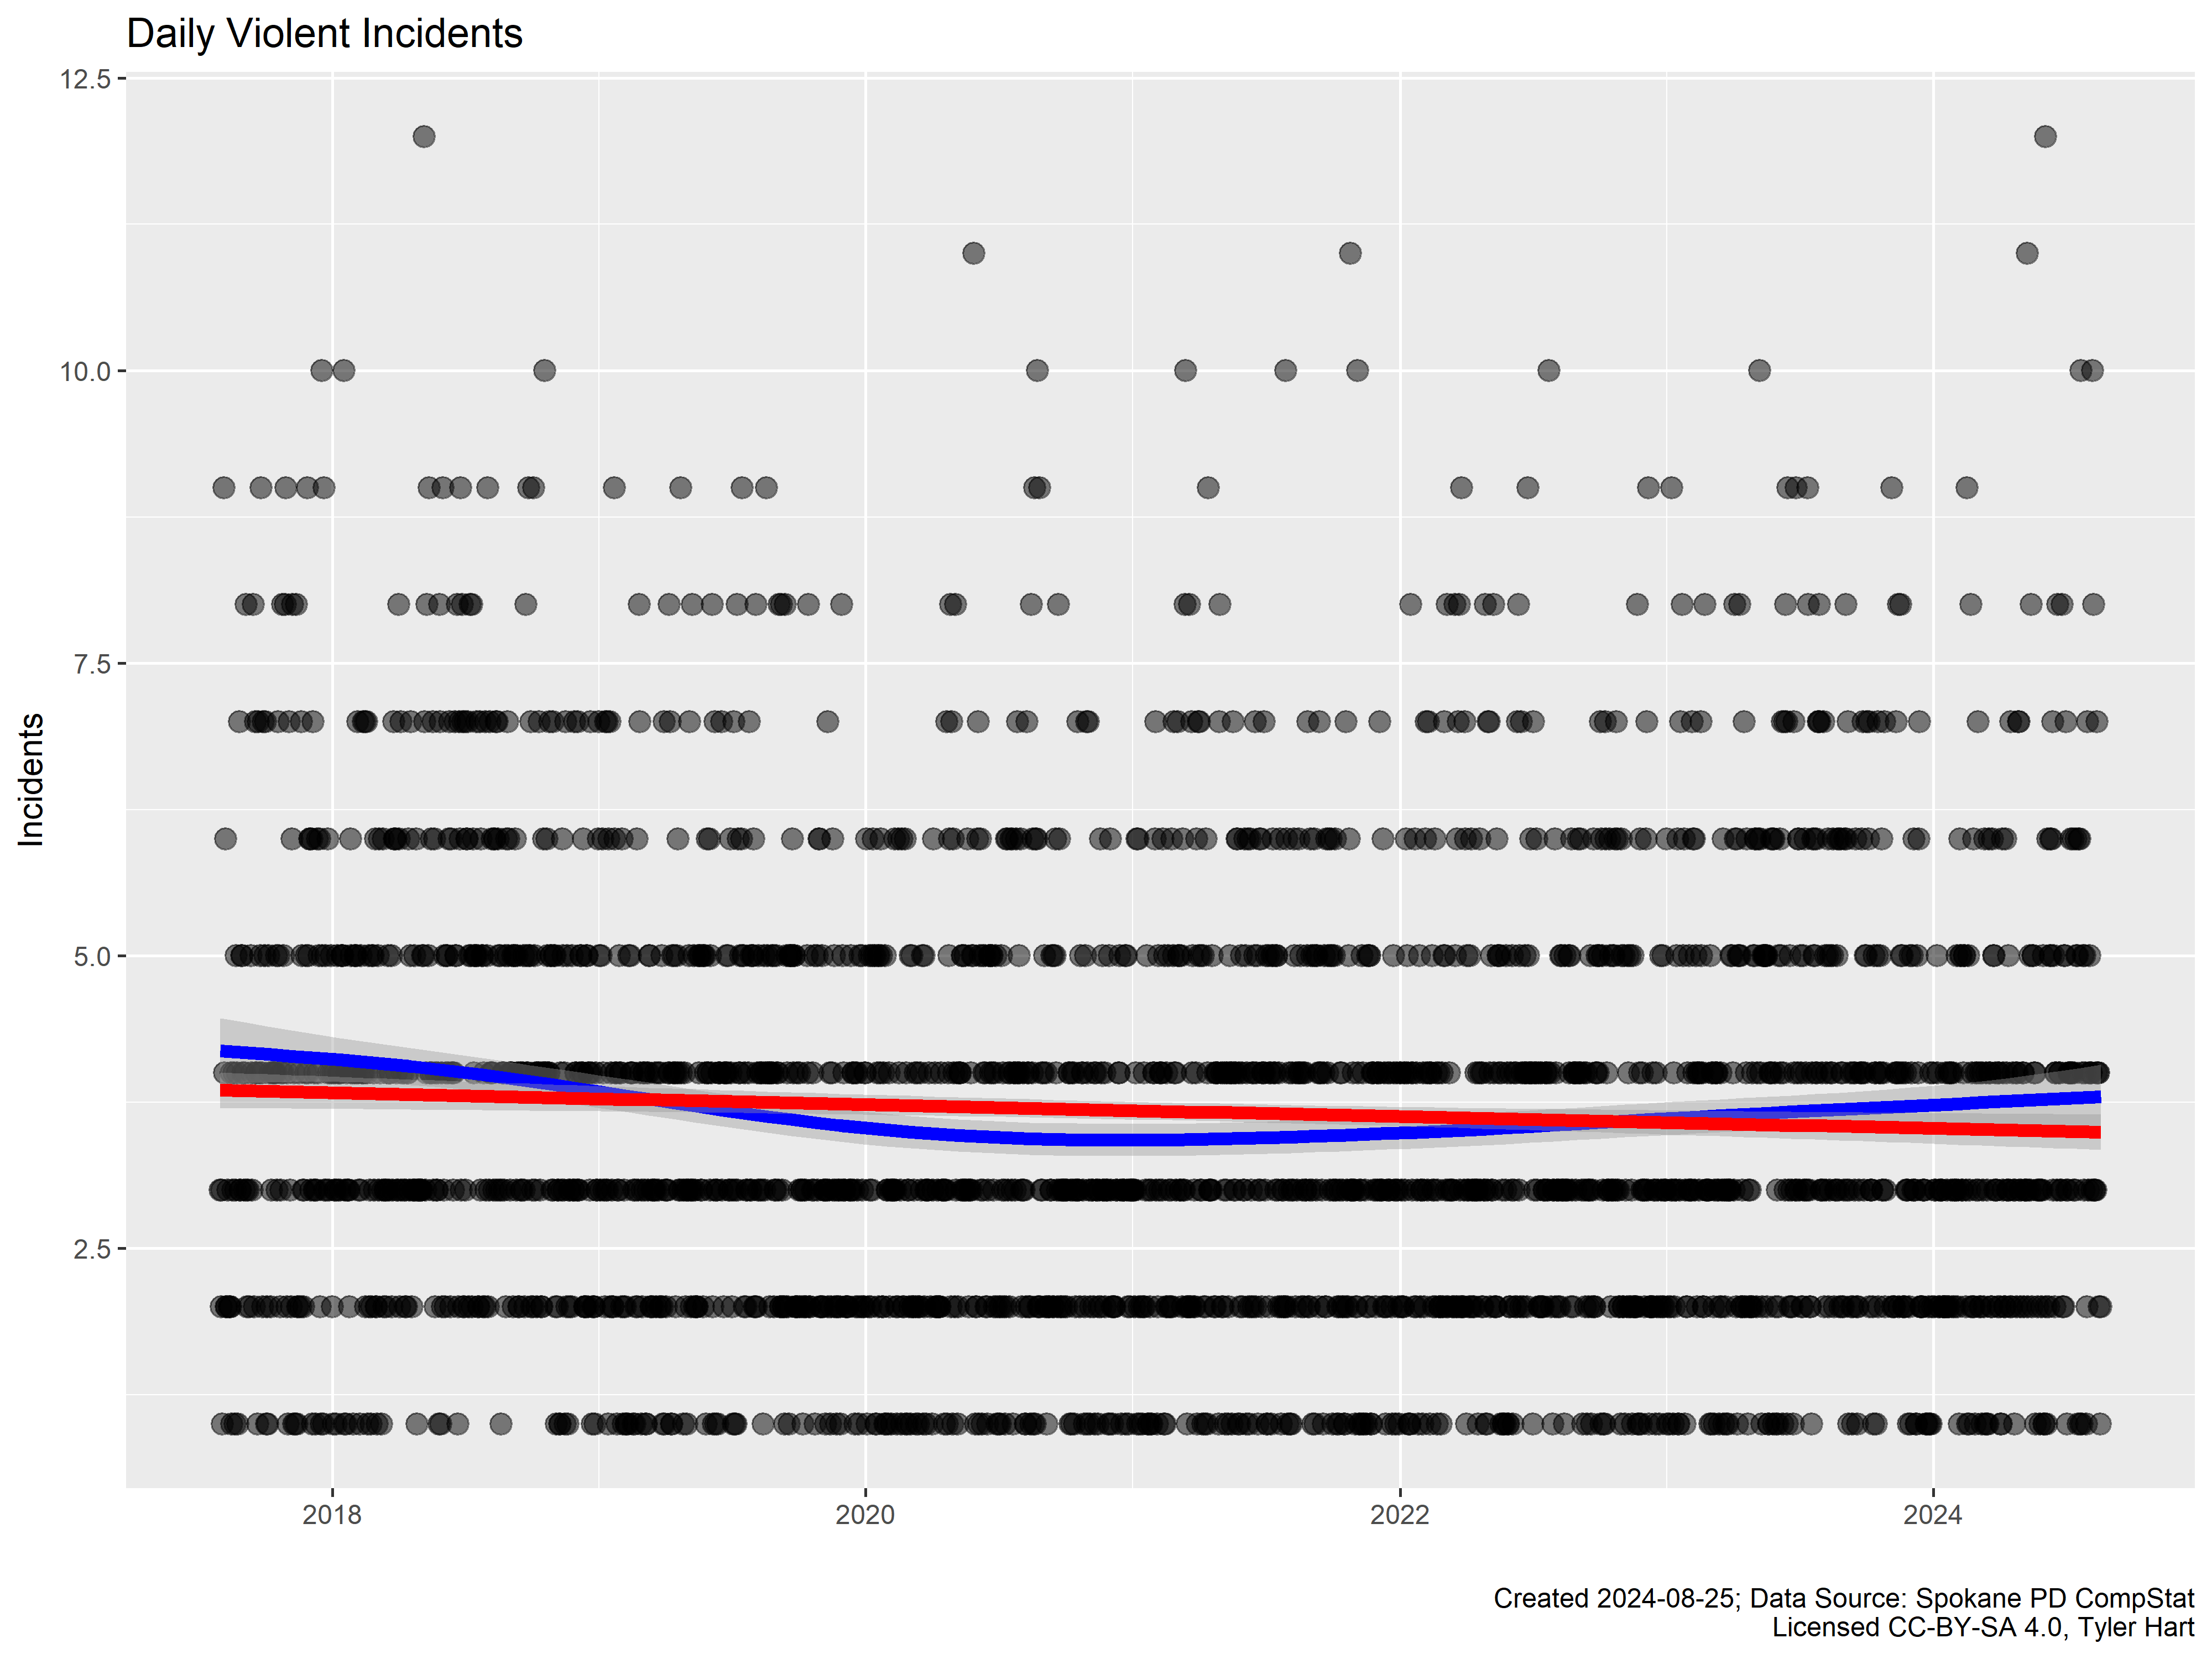
\includegraphics[width=\textwidth]{./figures/plot.violent_offenses_over_time-1} \end{center}

\begin{center}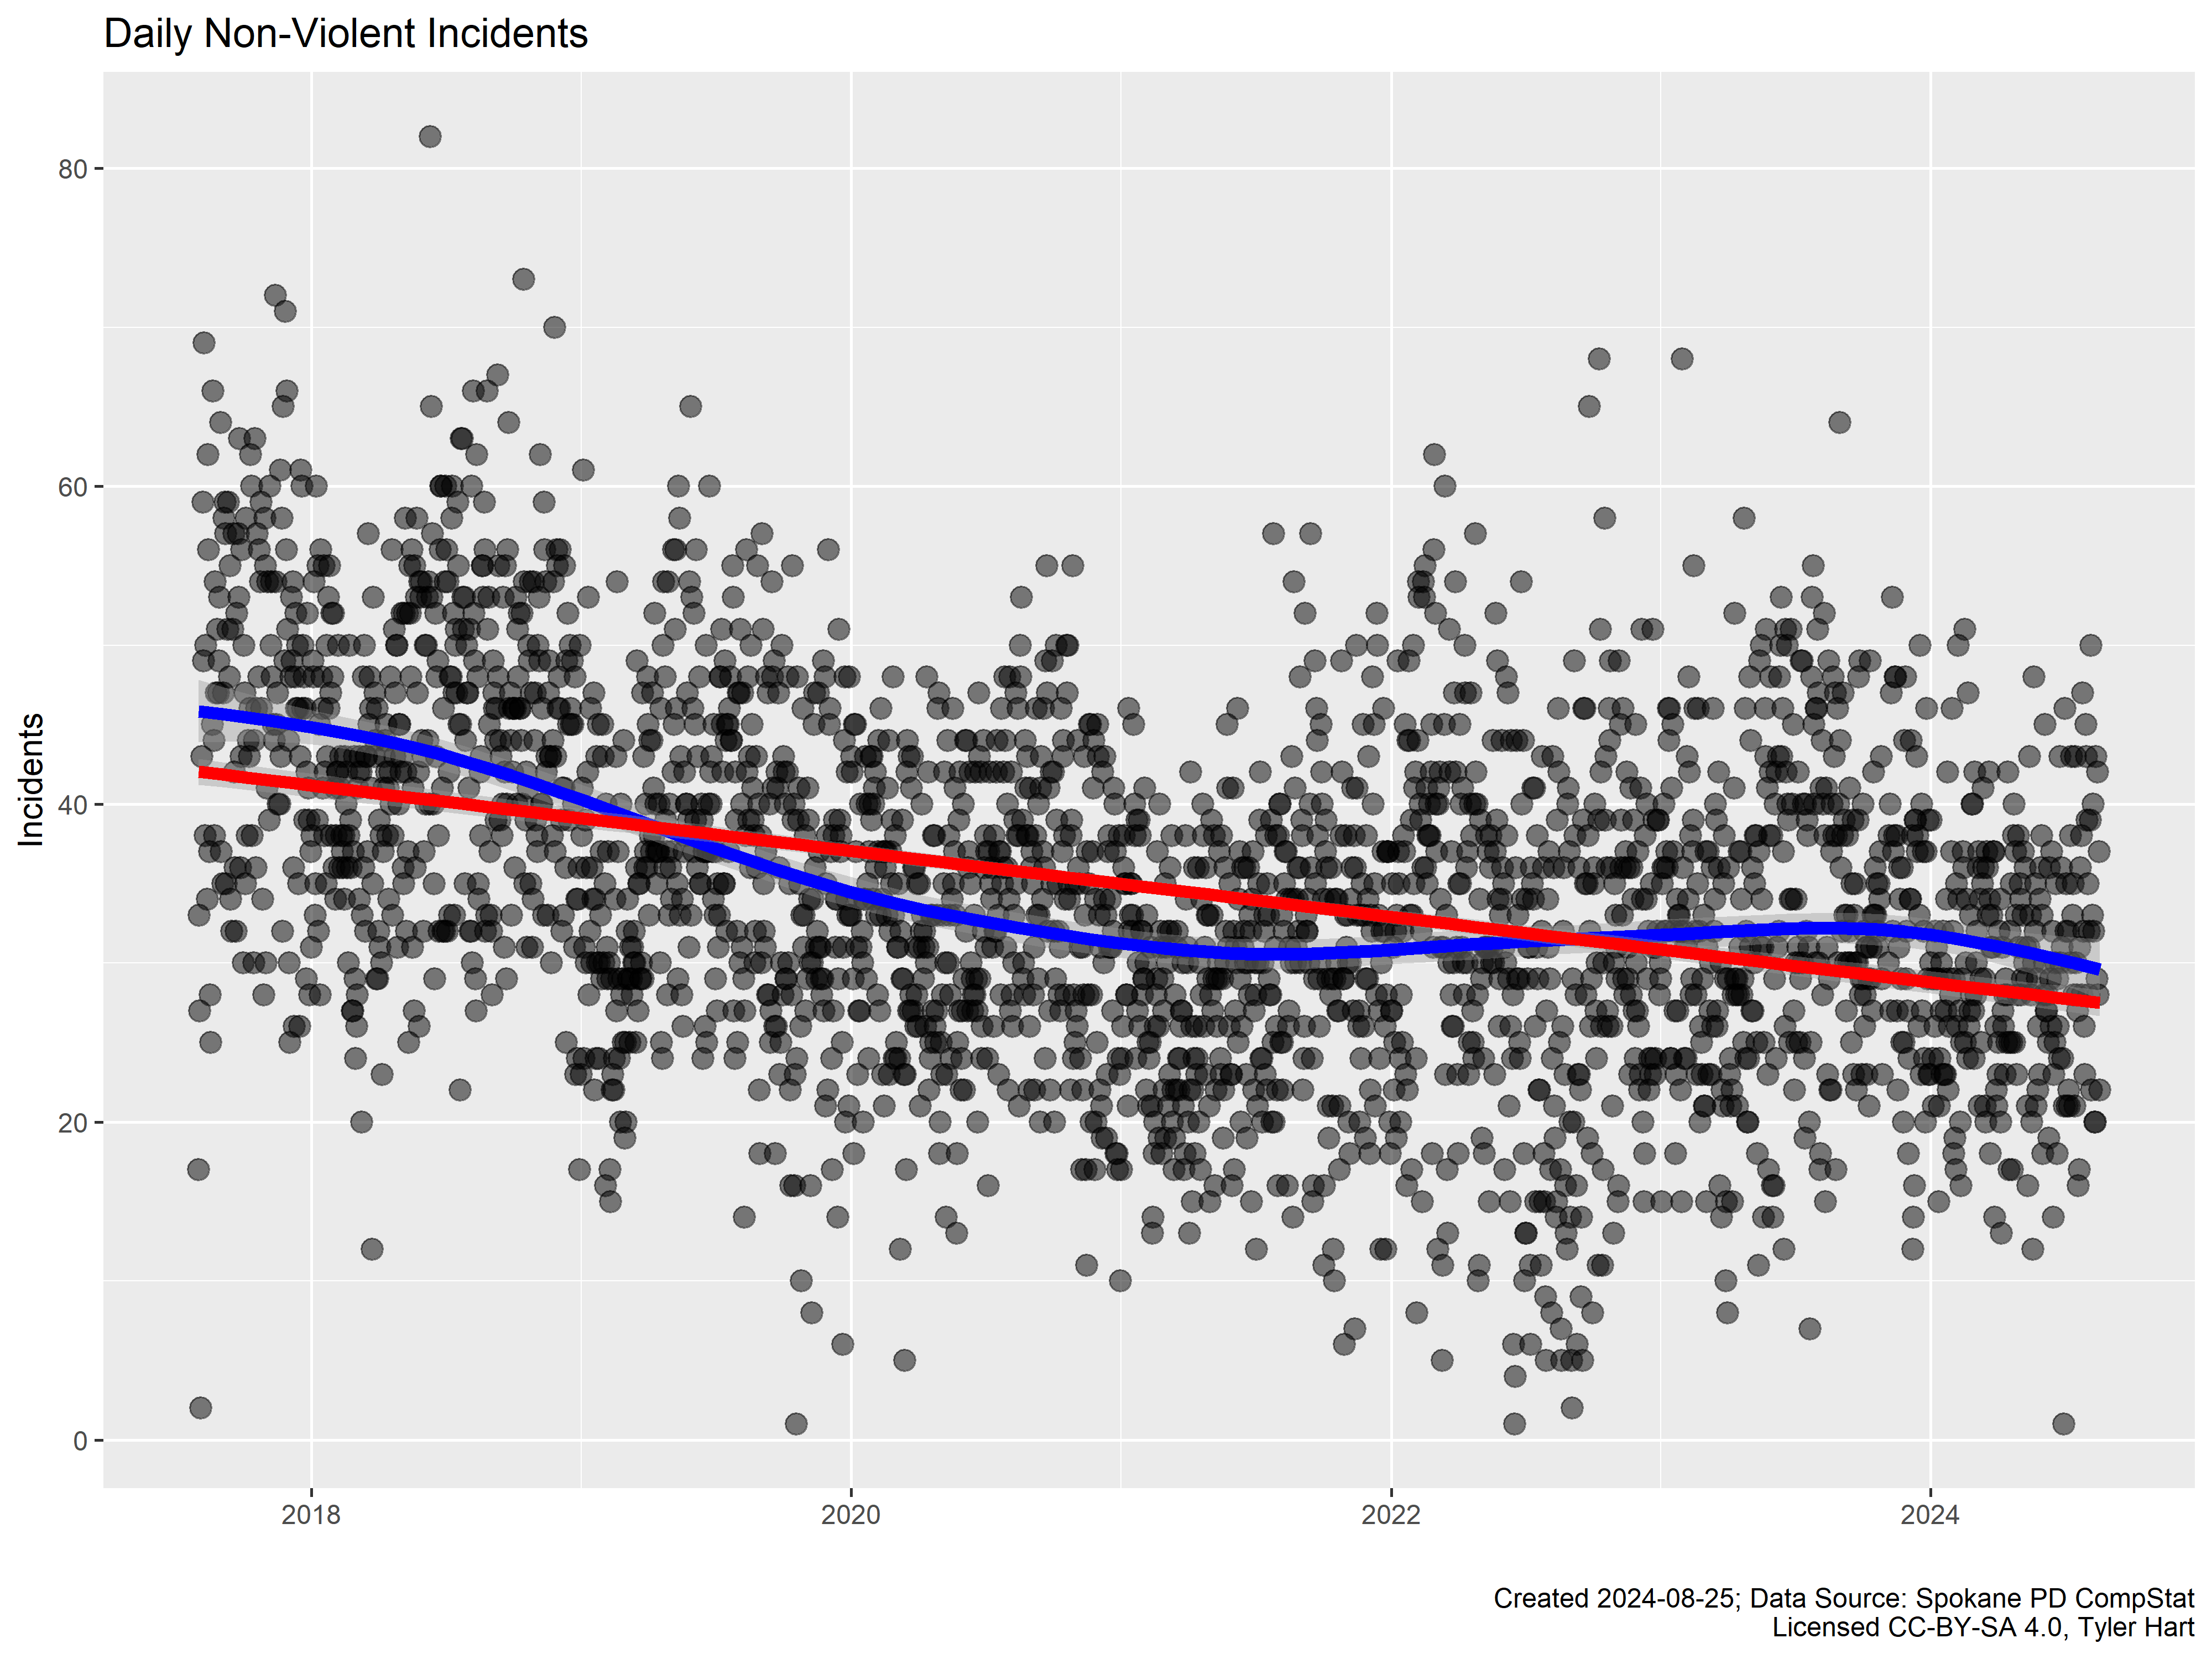
\includegraphics[width=\textwidth]{./figures/plot.non_violent_offenses_over_time-1} \end{center}

\begin{center}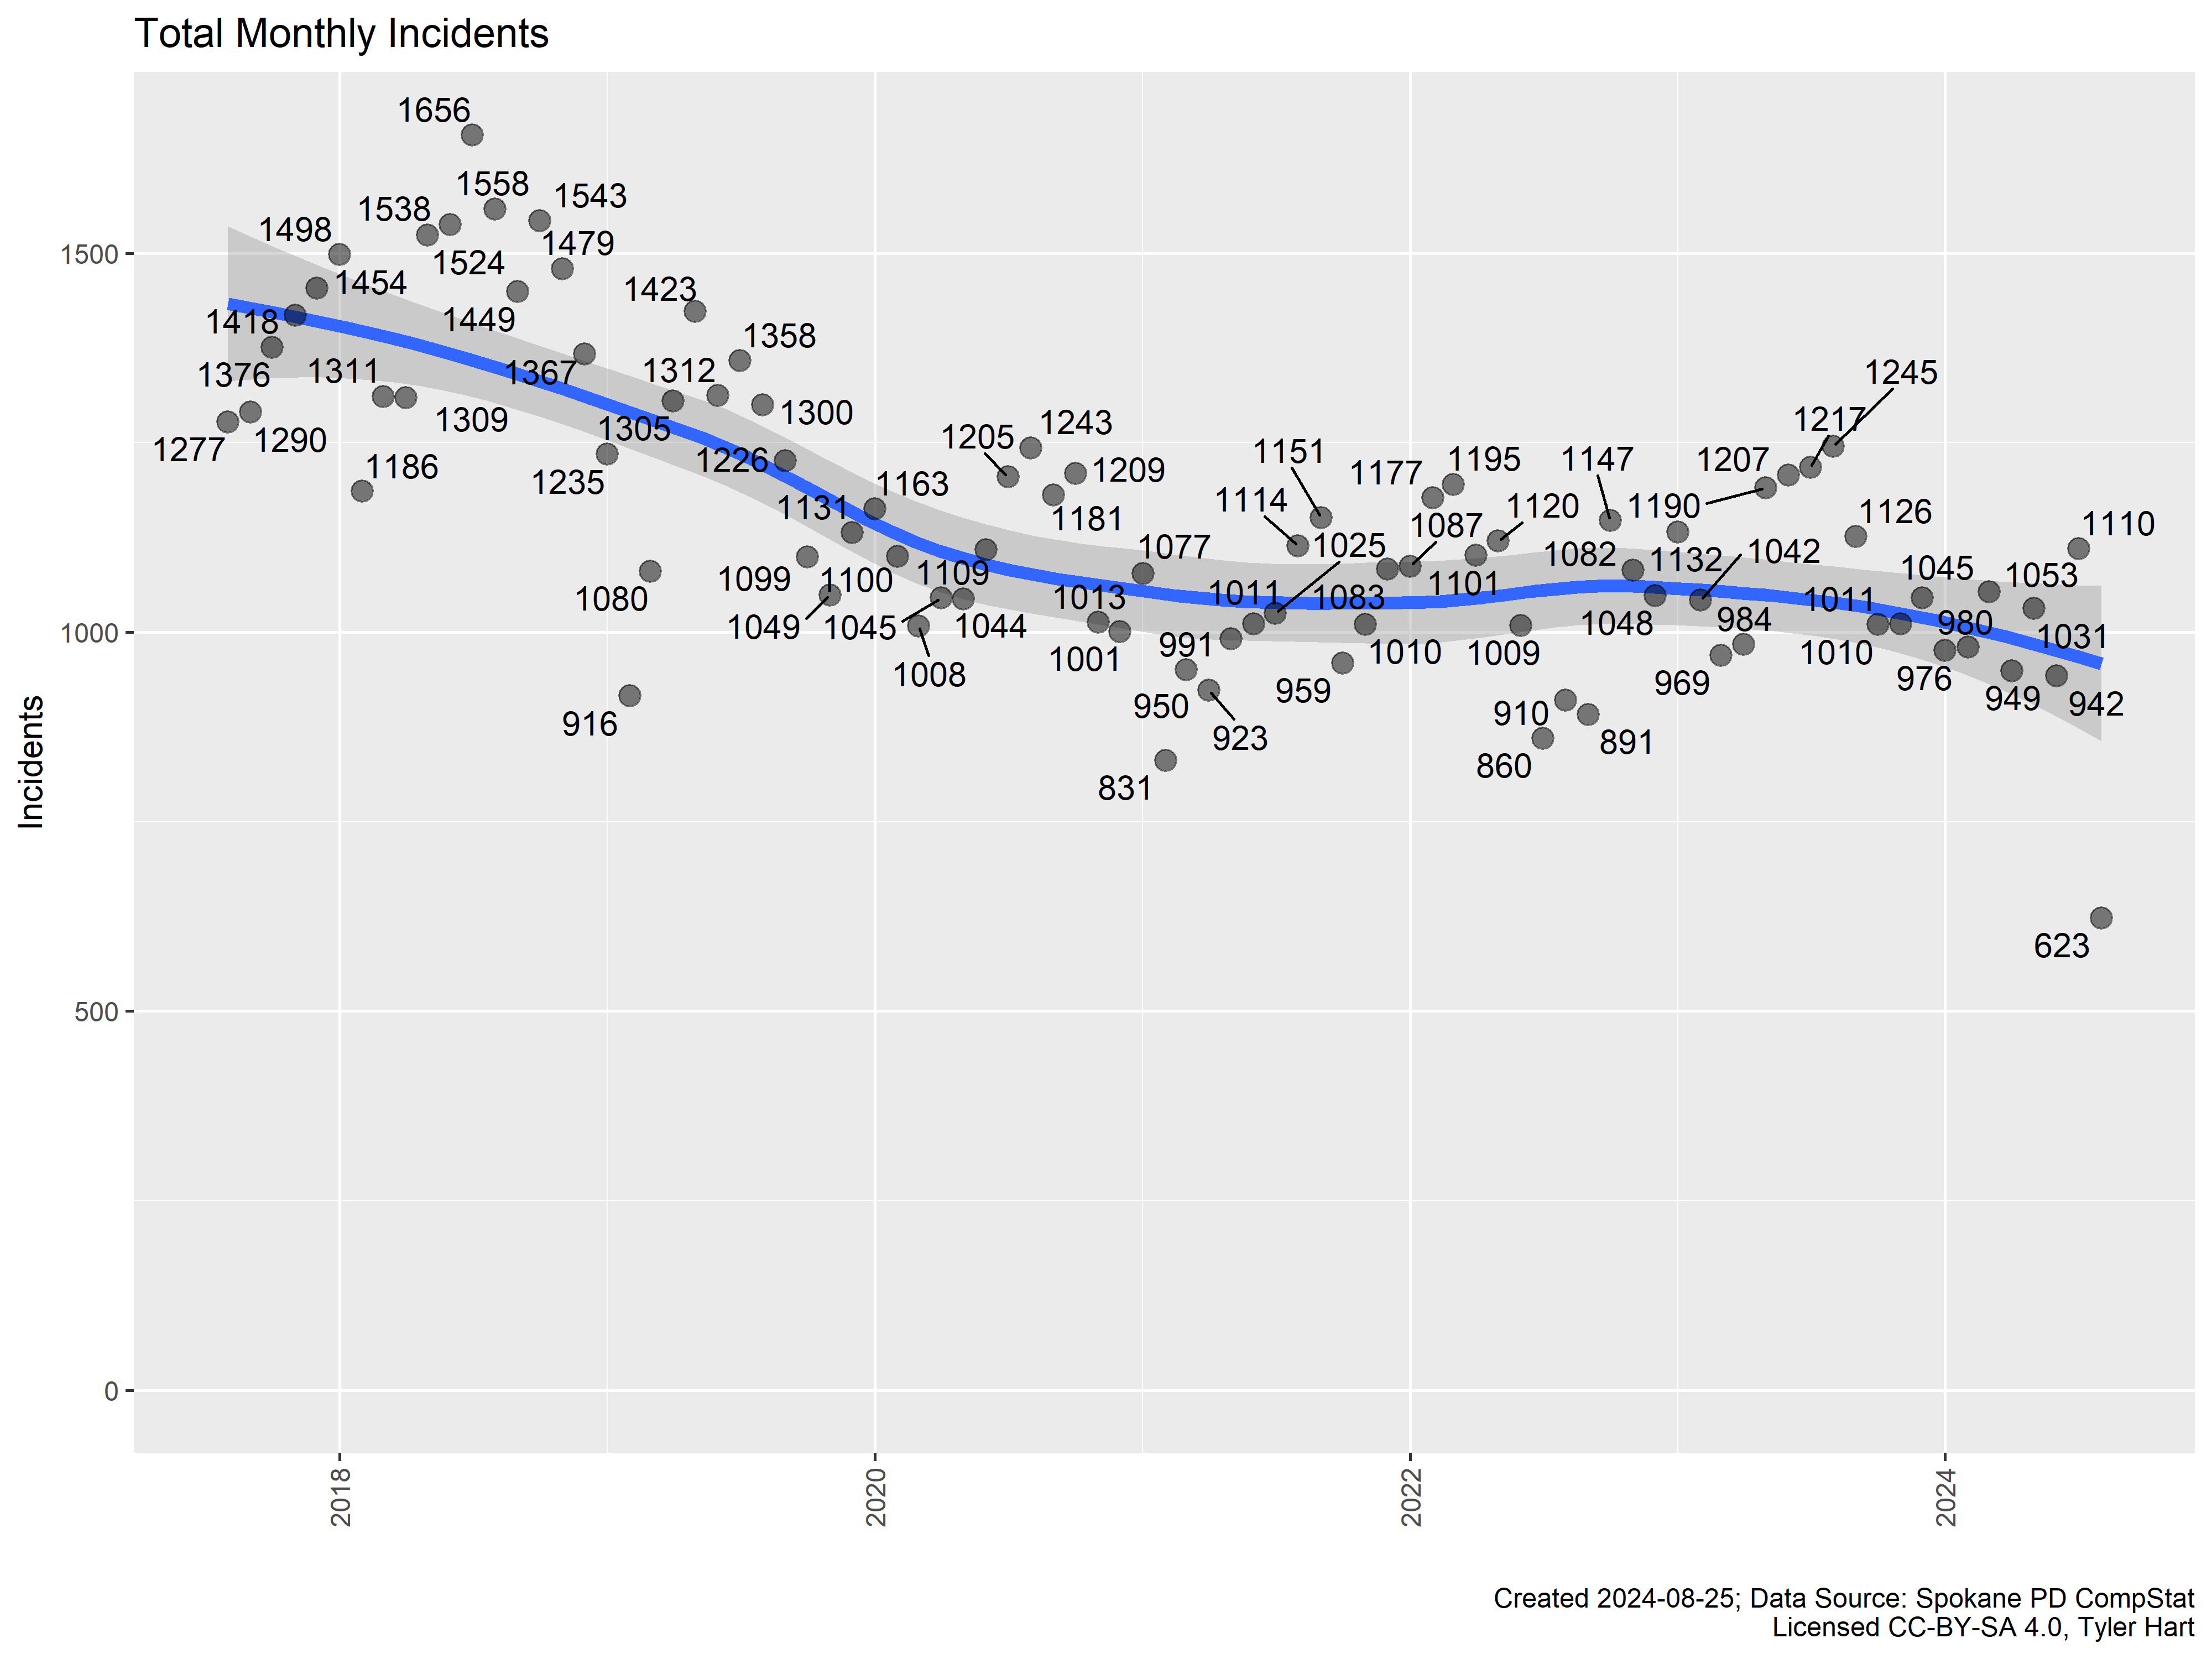
\includegraphics[width=\textwidth]{./figures/plot.monthly_offense_totals-1} \end{center}

\begin{center}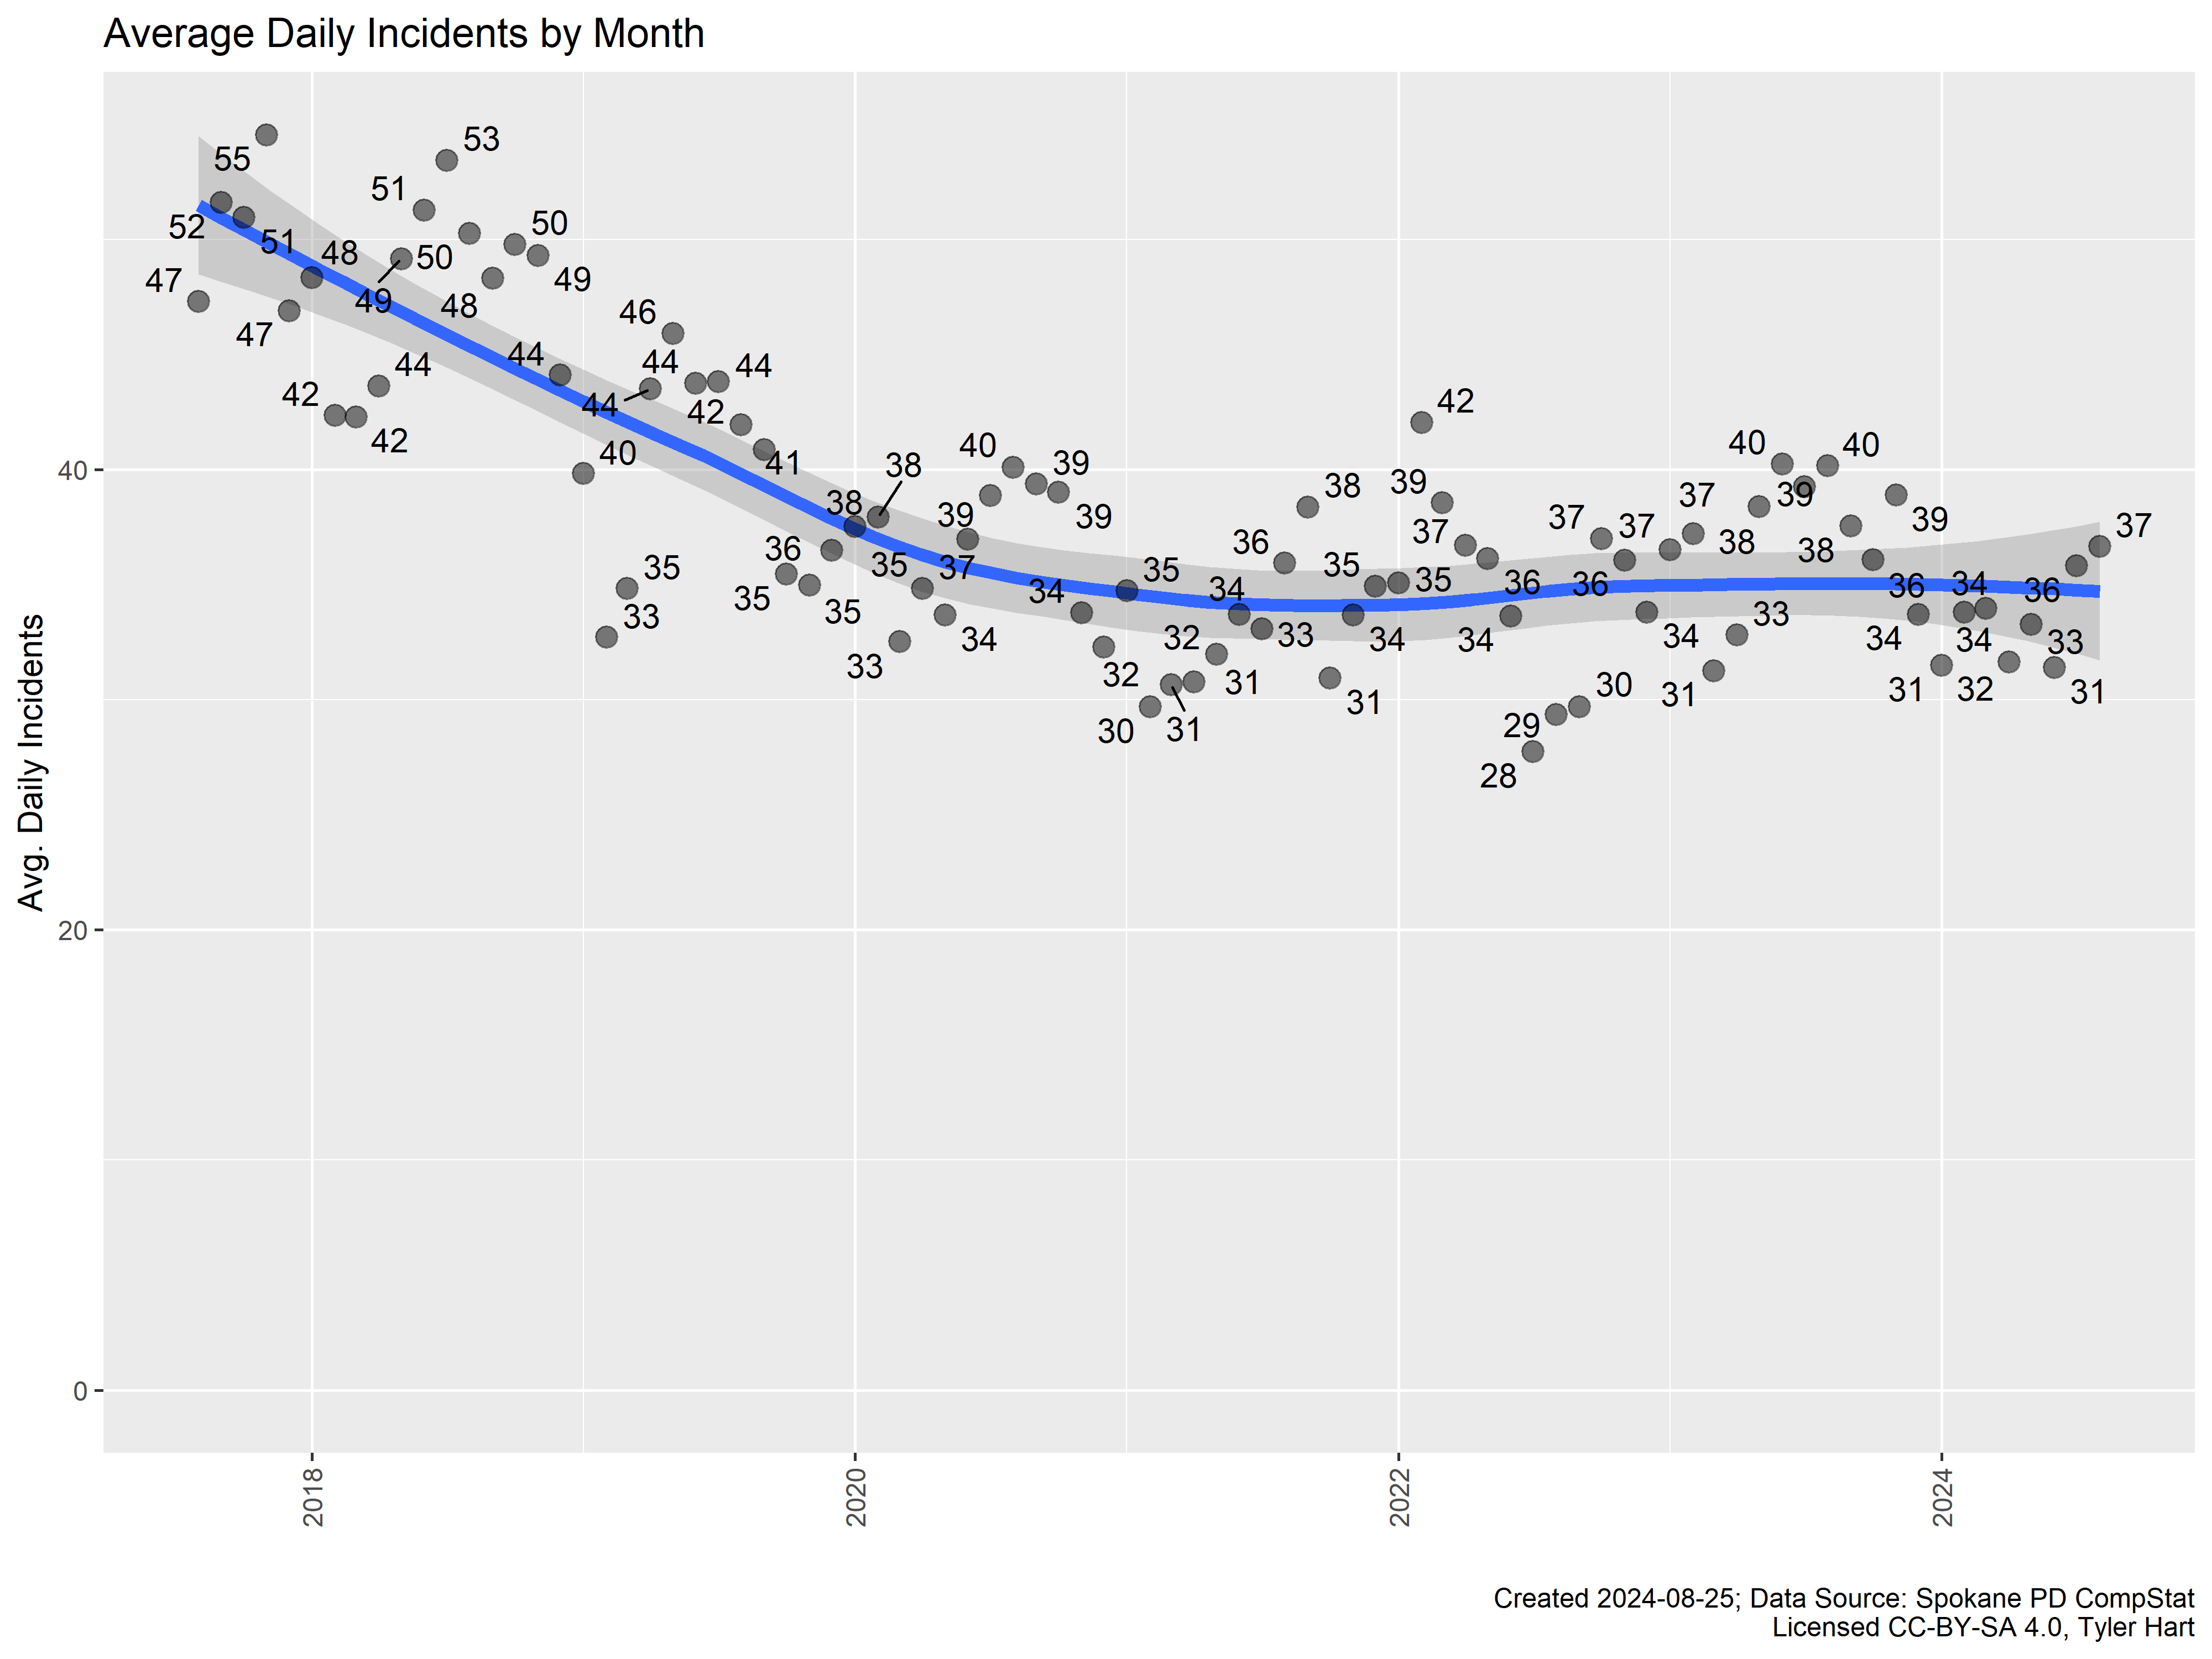
\includegraphics[width=\textwidth]{./figures/plot.avg_daily_offenses_by_month-1} \end{center}

\begin{center}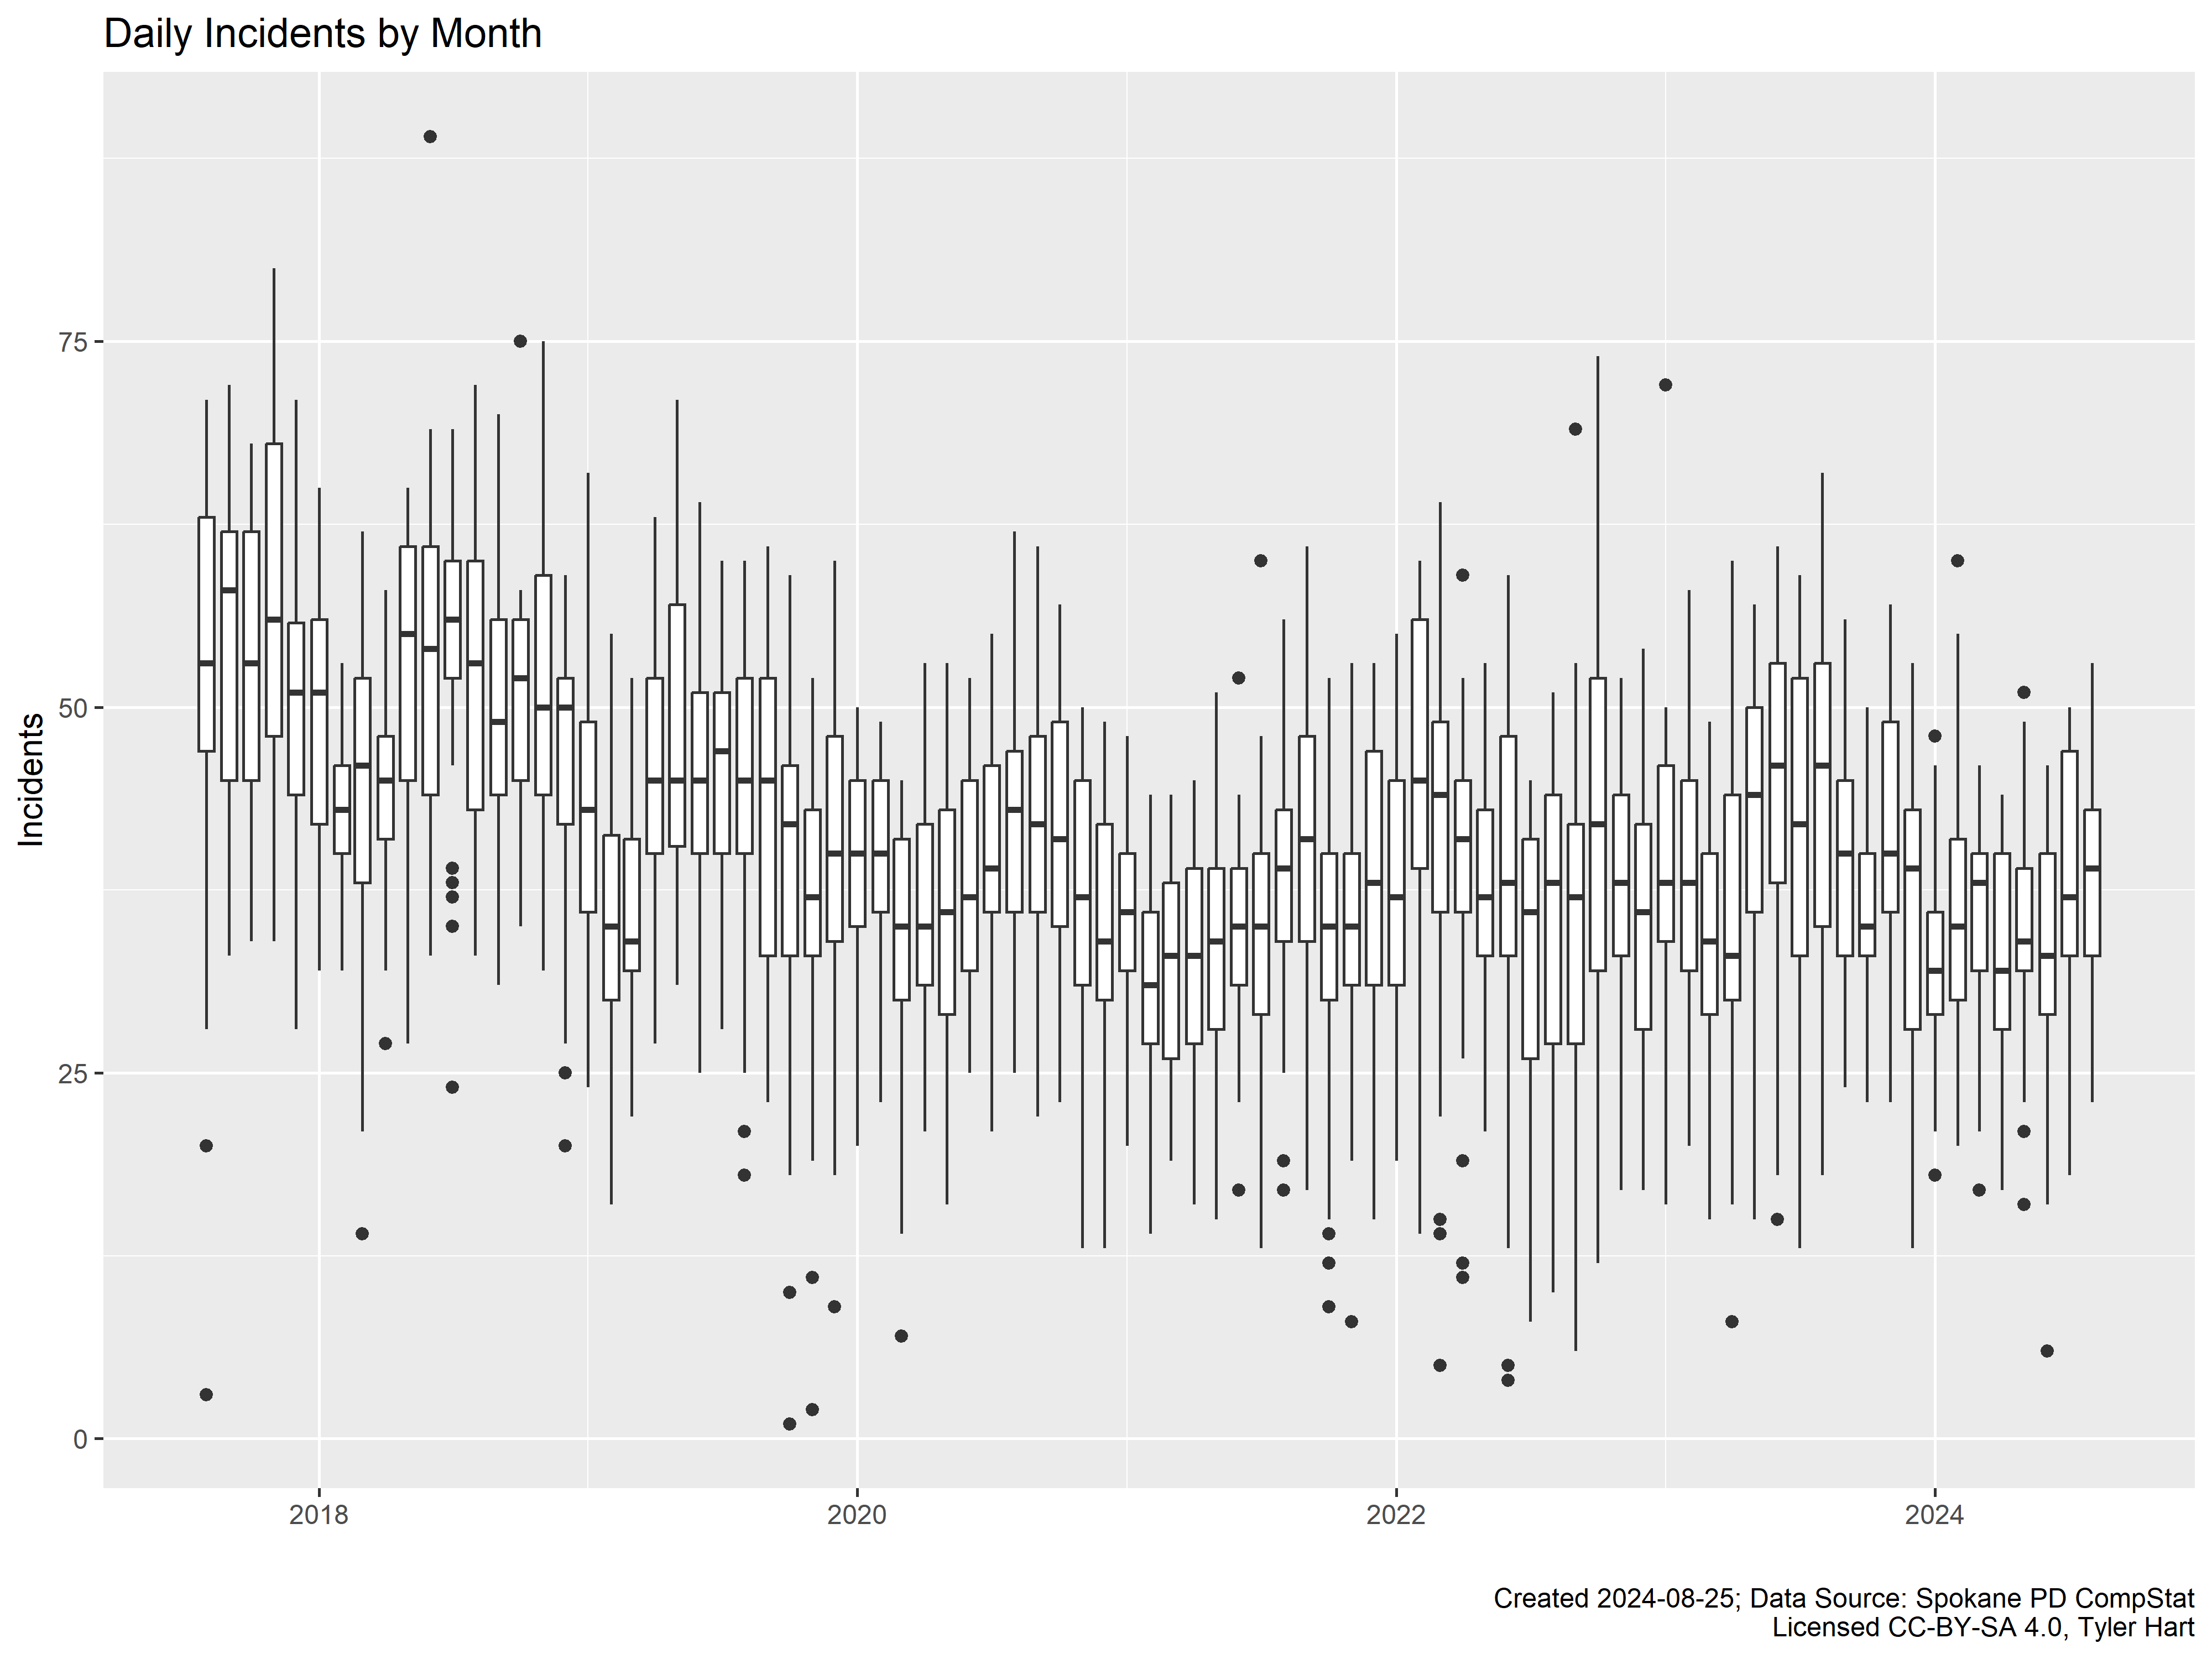
\includegraphics[width=\textwidth]{./figures/plot.boxplot_avg_daily_by_month-1} \end{center}

\begin{center}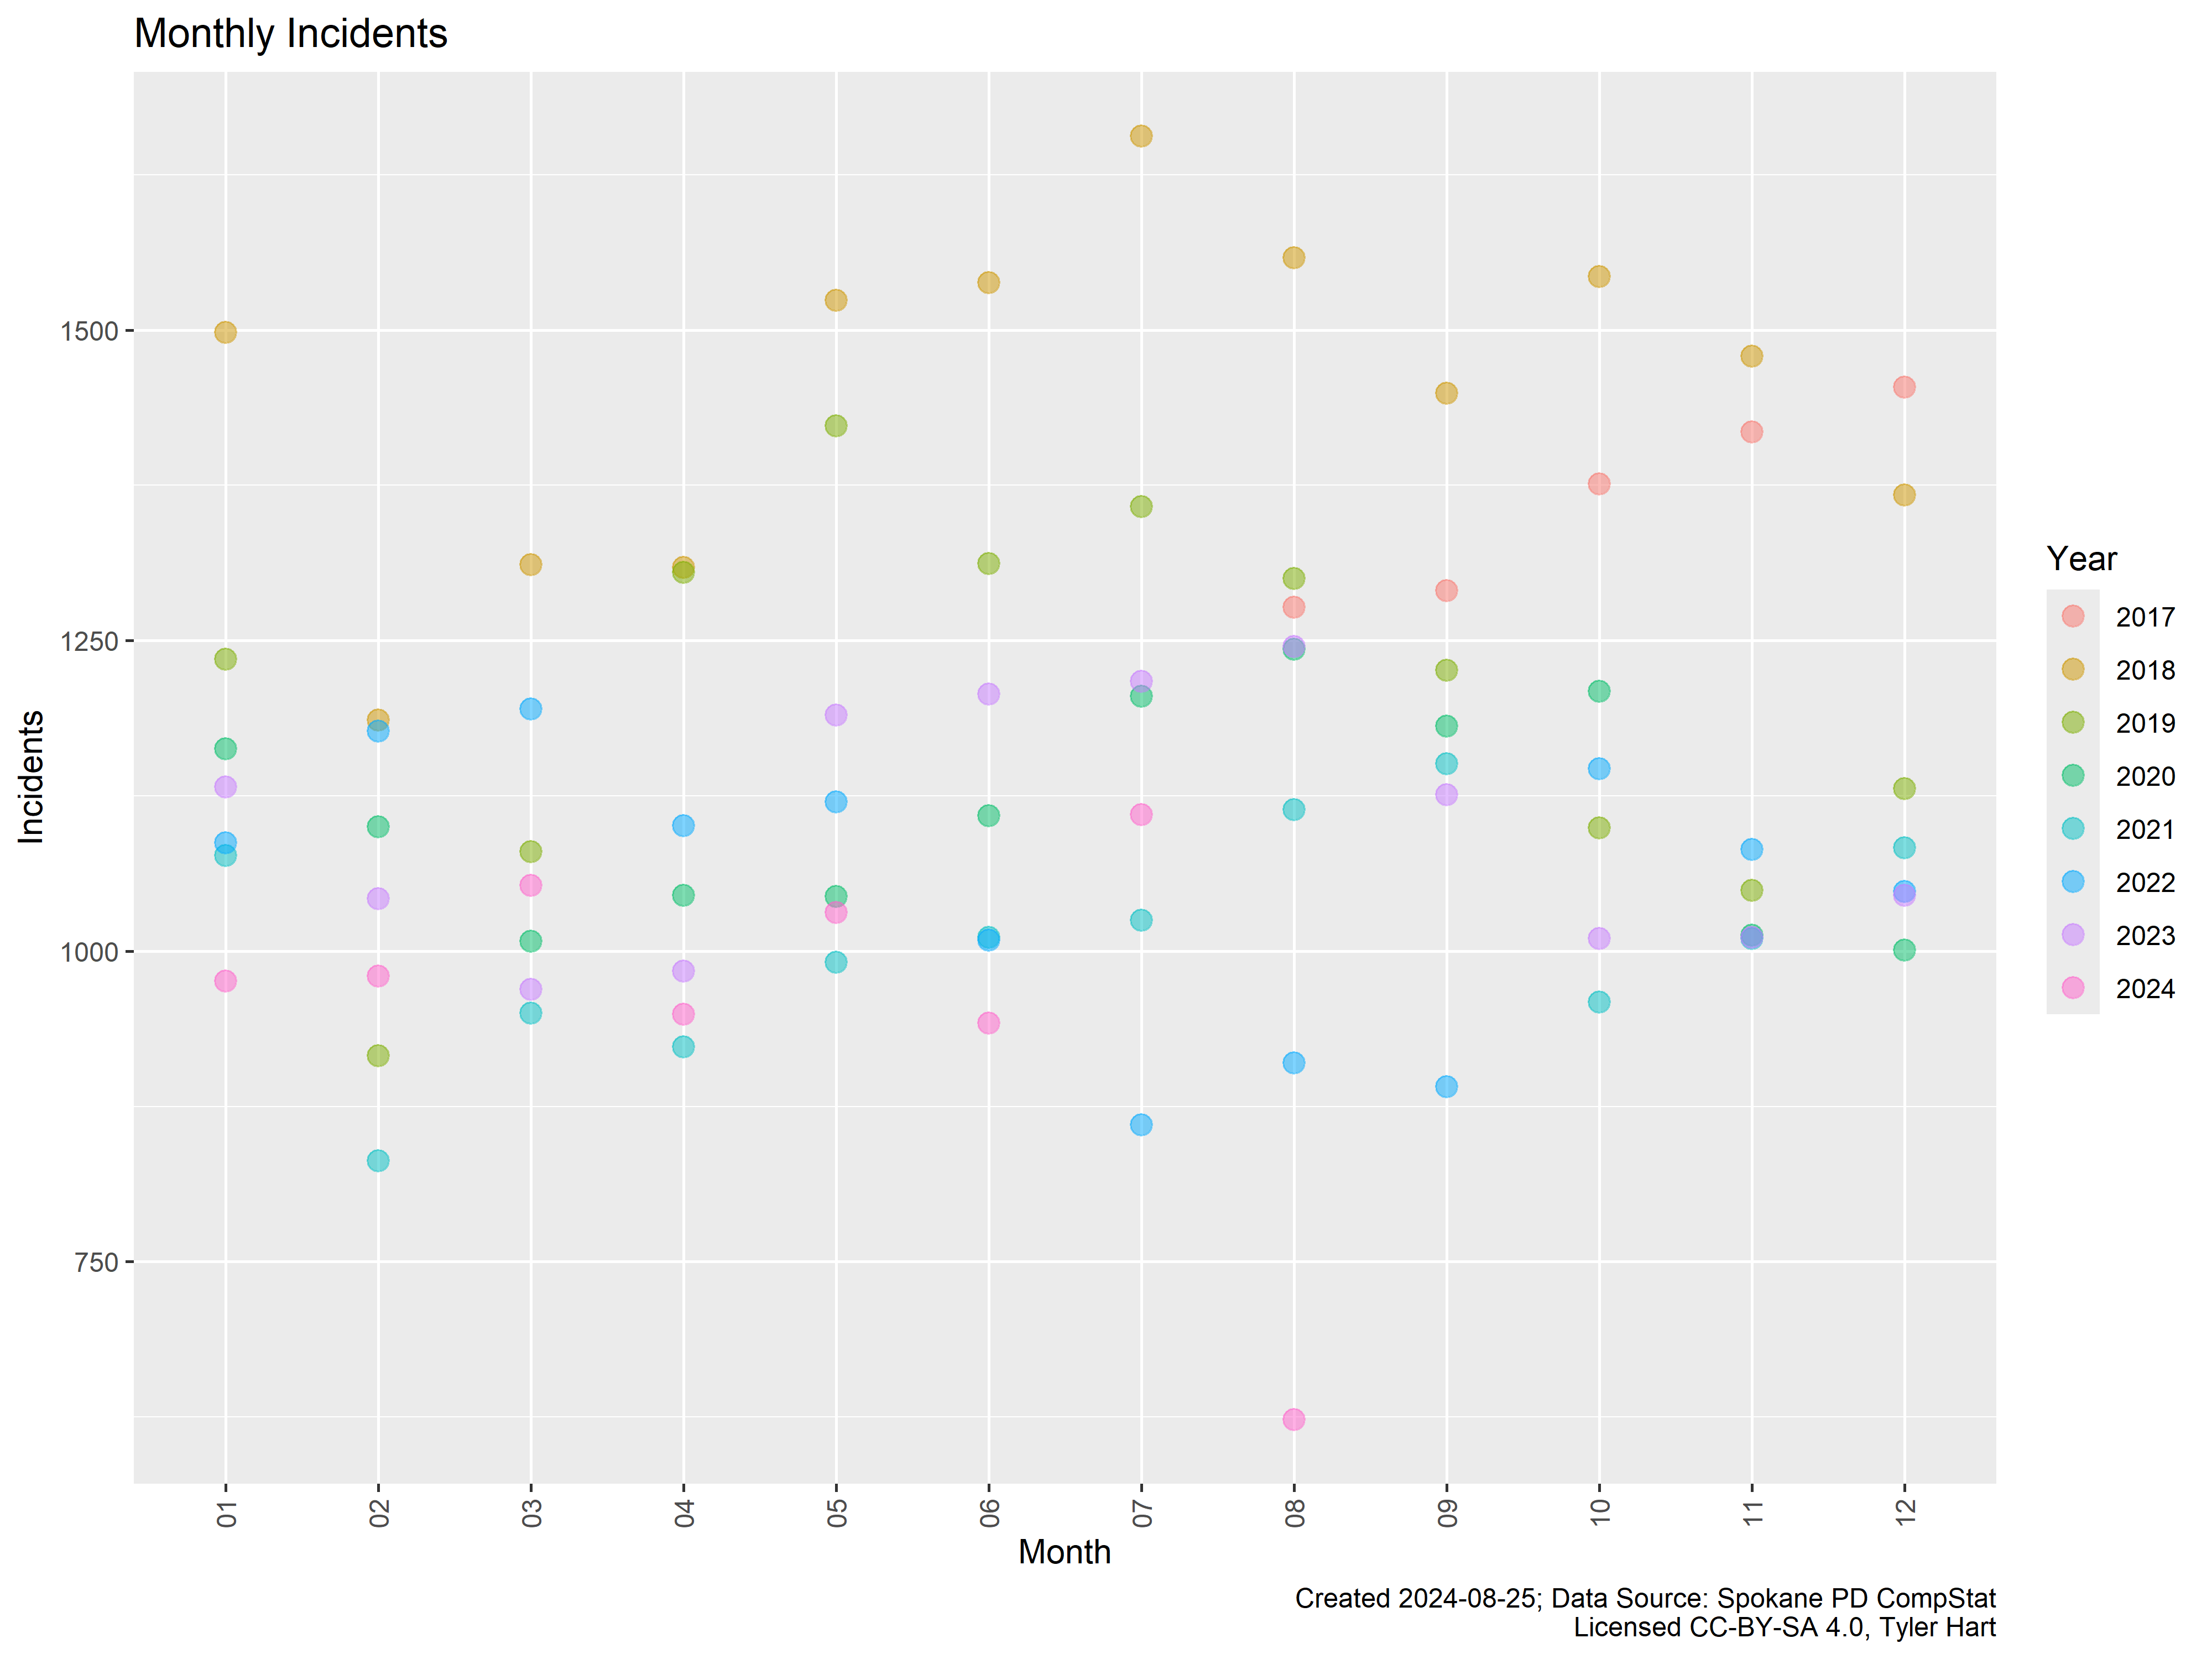
\includegraphics[width=\textwidth]{./figures/plot.monthly_offense_comparisons-1} \end{center}

\begin{center}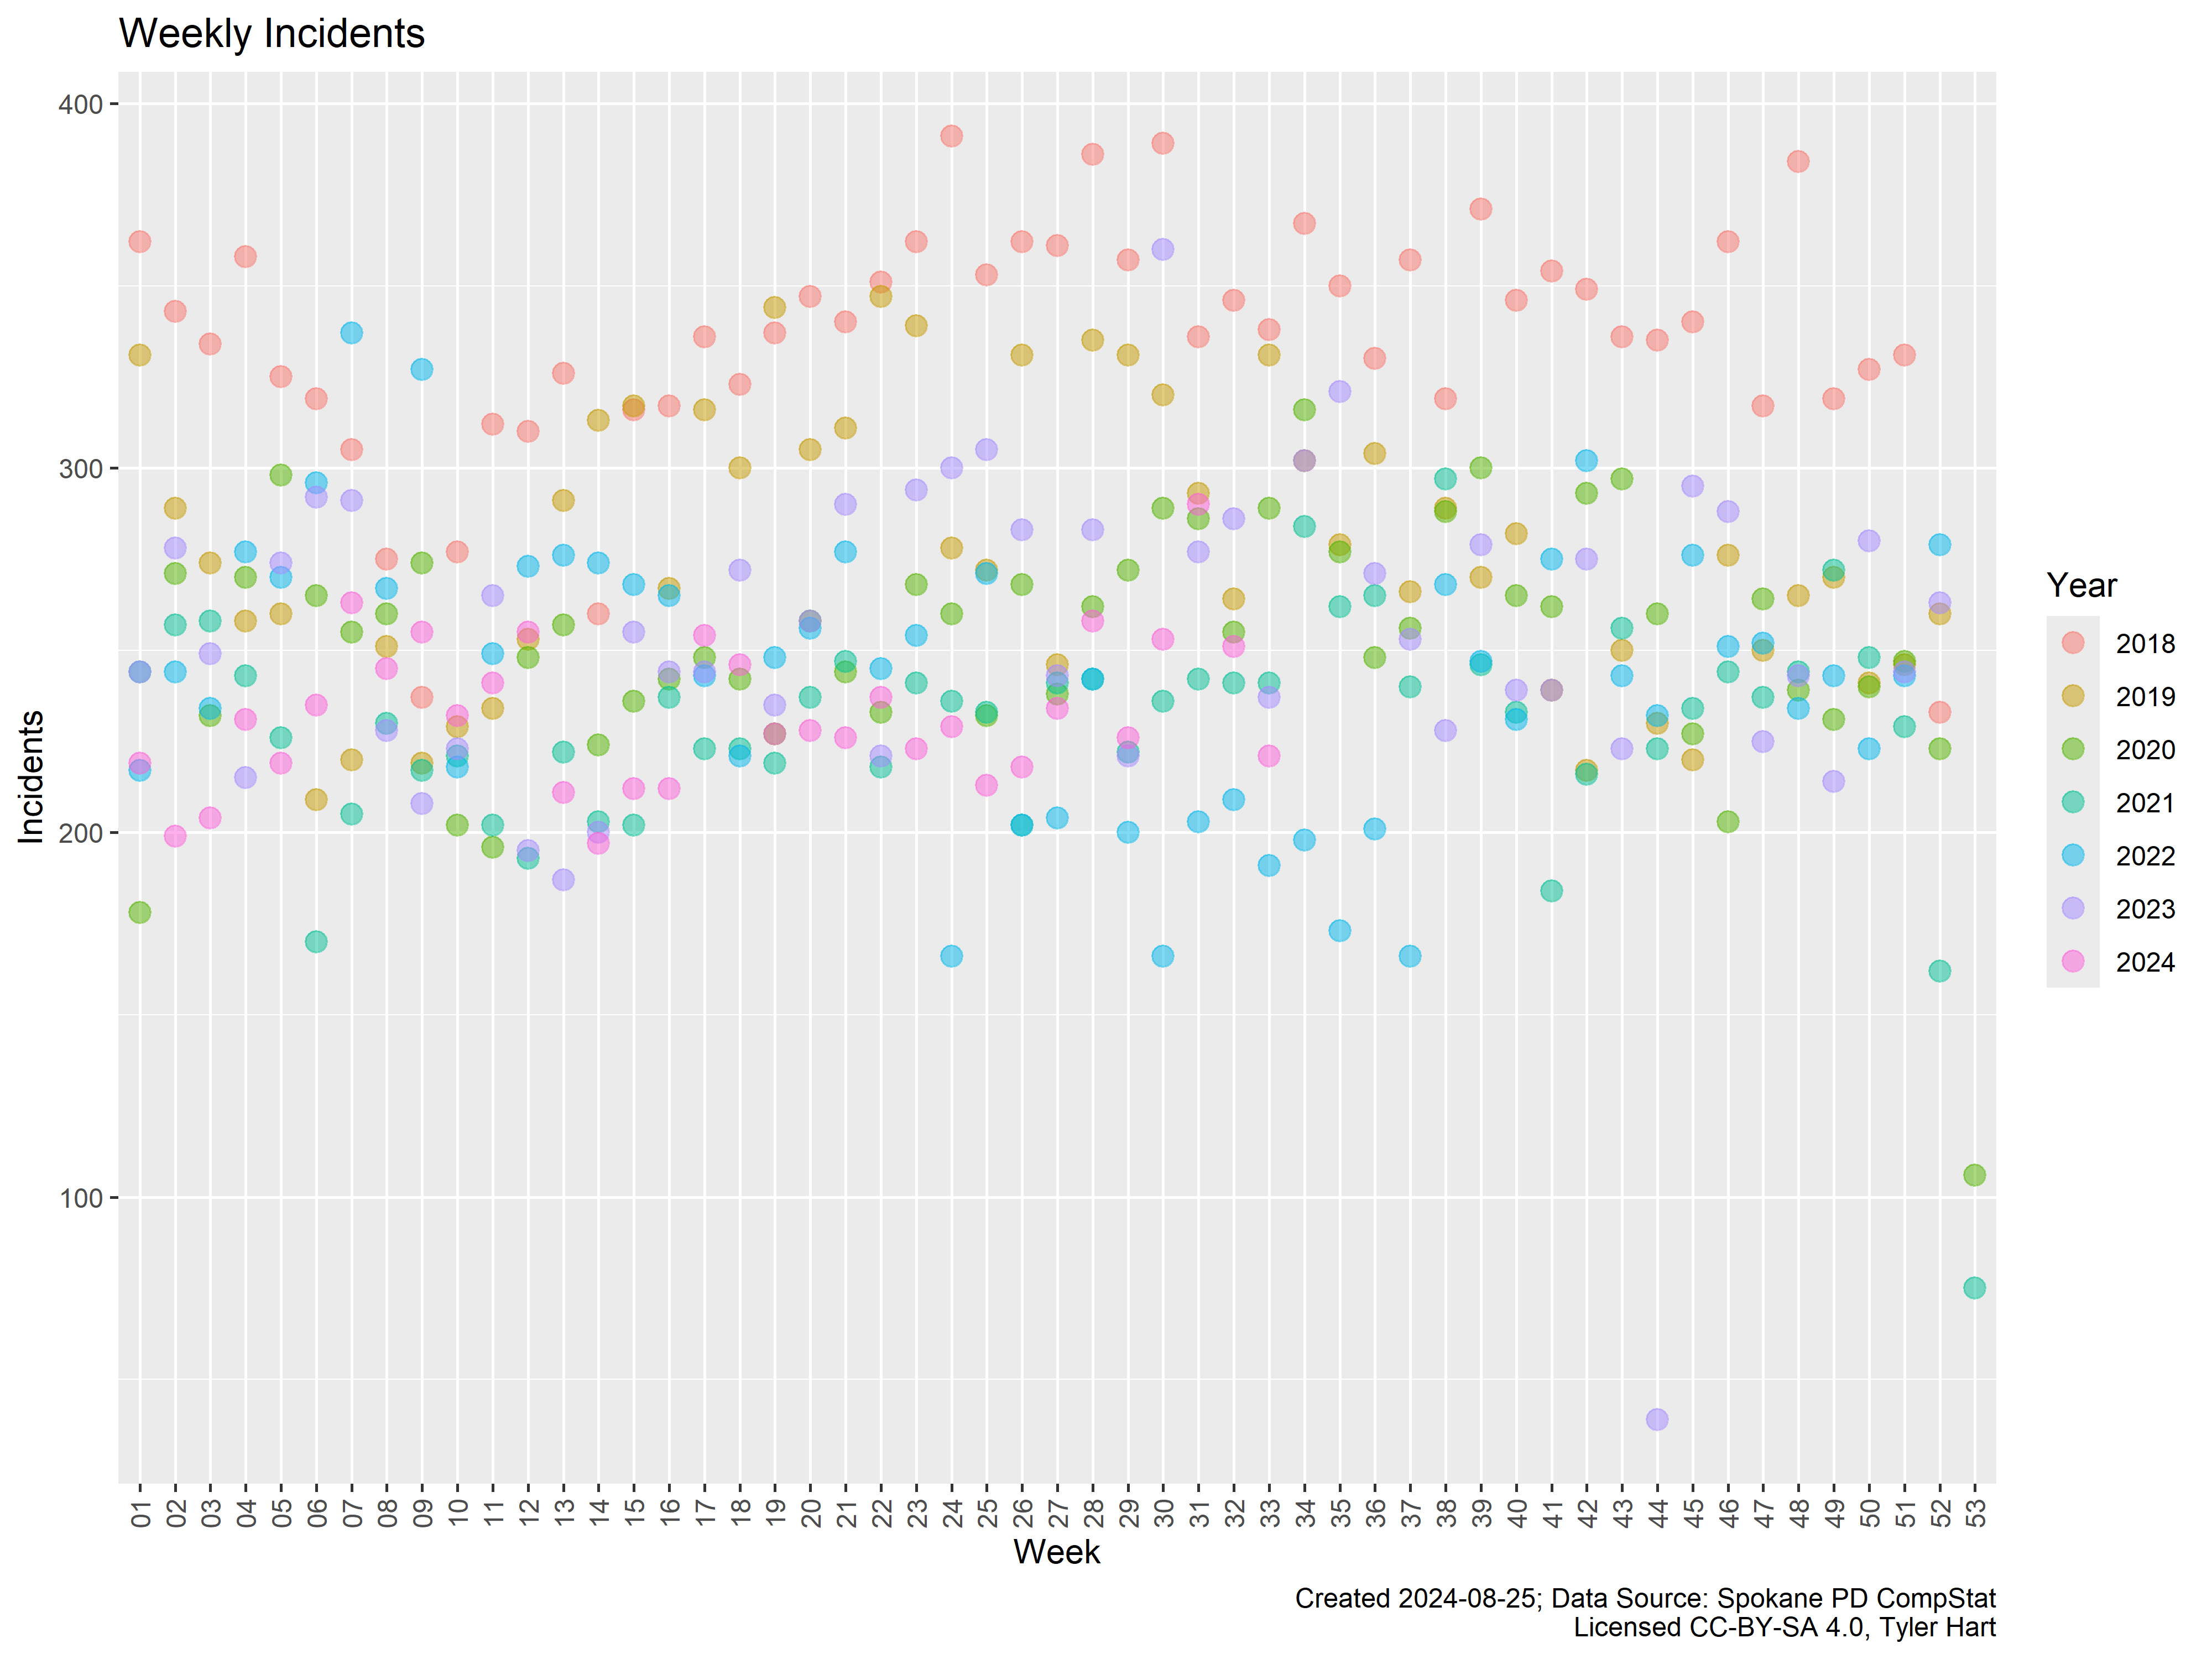
\includegraphics[width=\textwidth]{./figures/plot.weekly_offense_comparisons-1} \end{center}

\begin{center}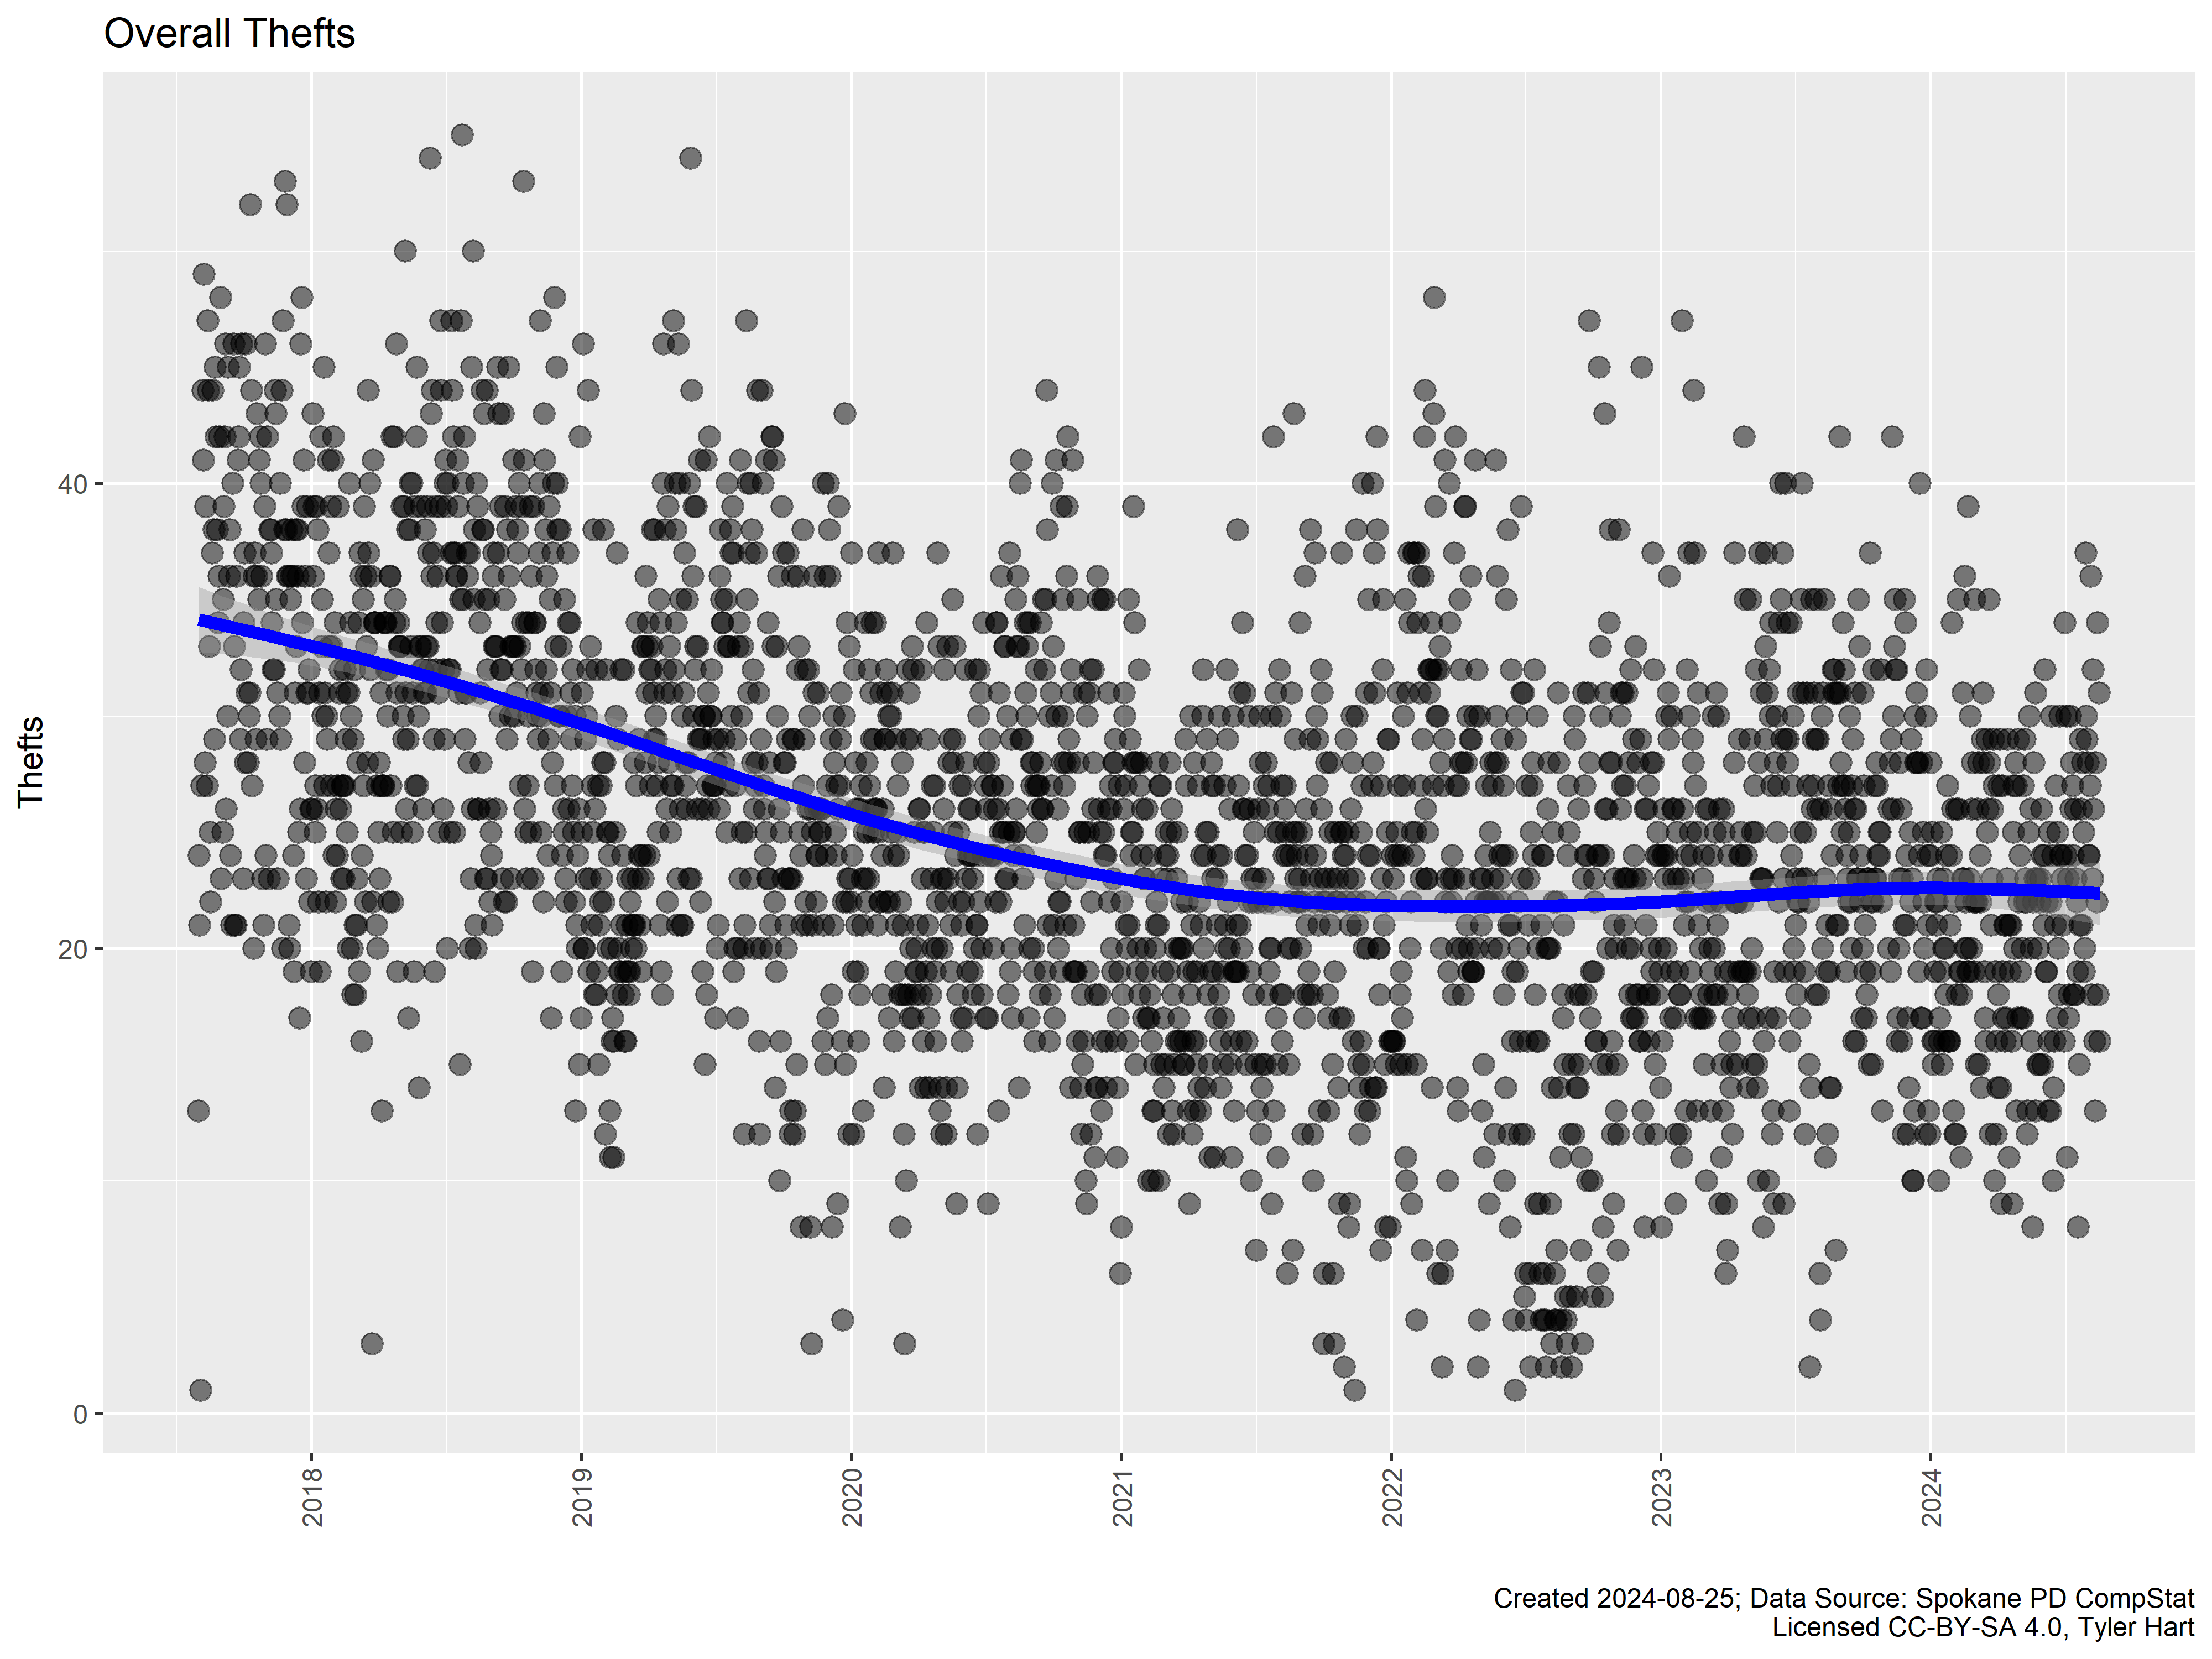
\includegraphics[width=\textwidth]{./figures/plot.theft_over_time-1} \end{center}

\begin{center}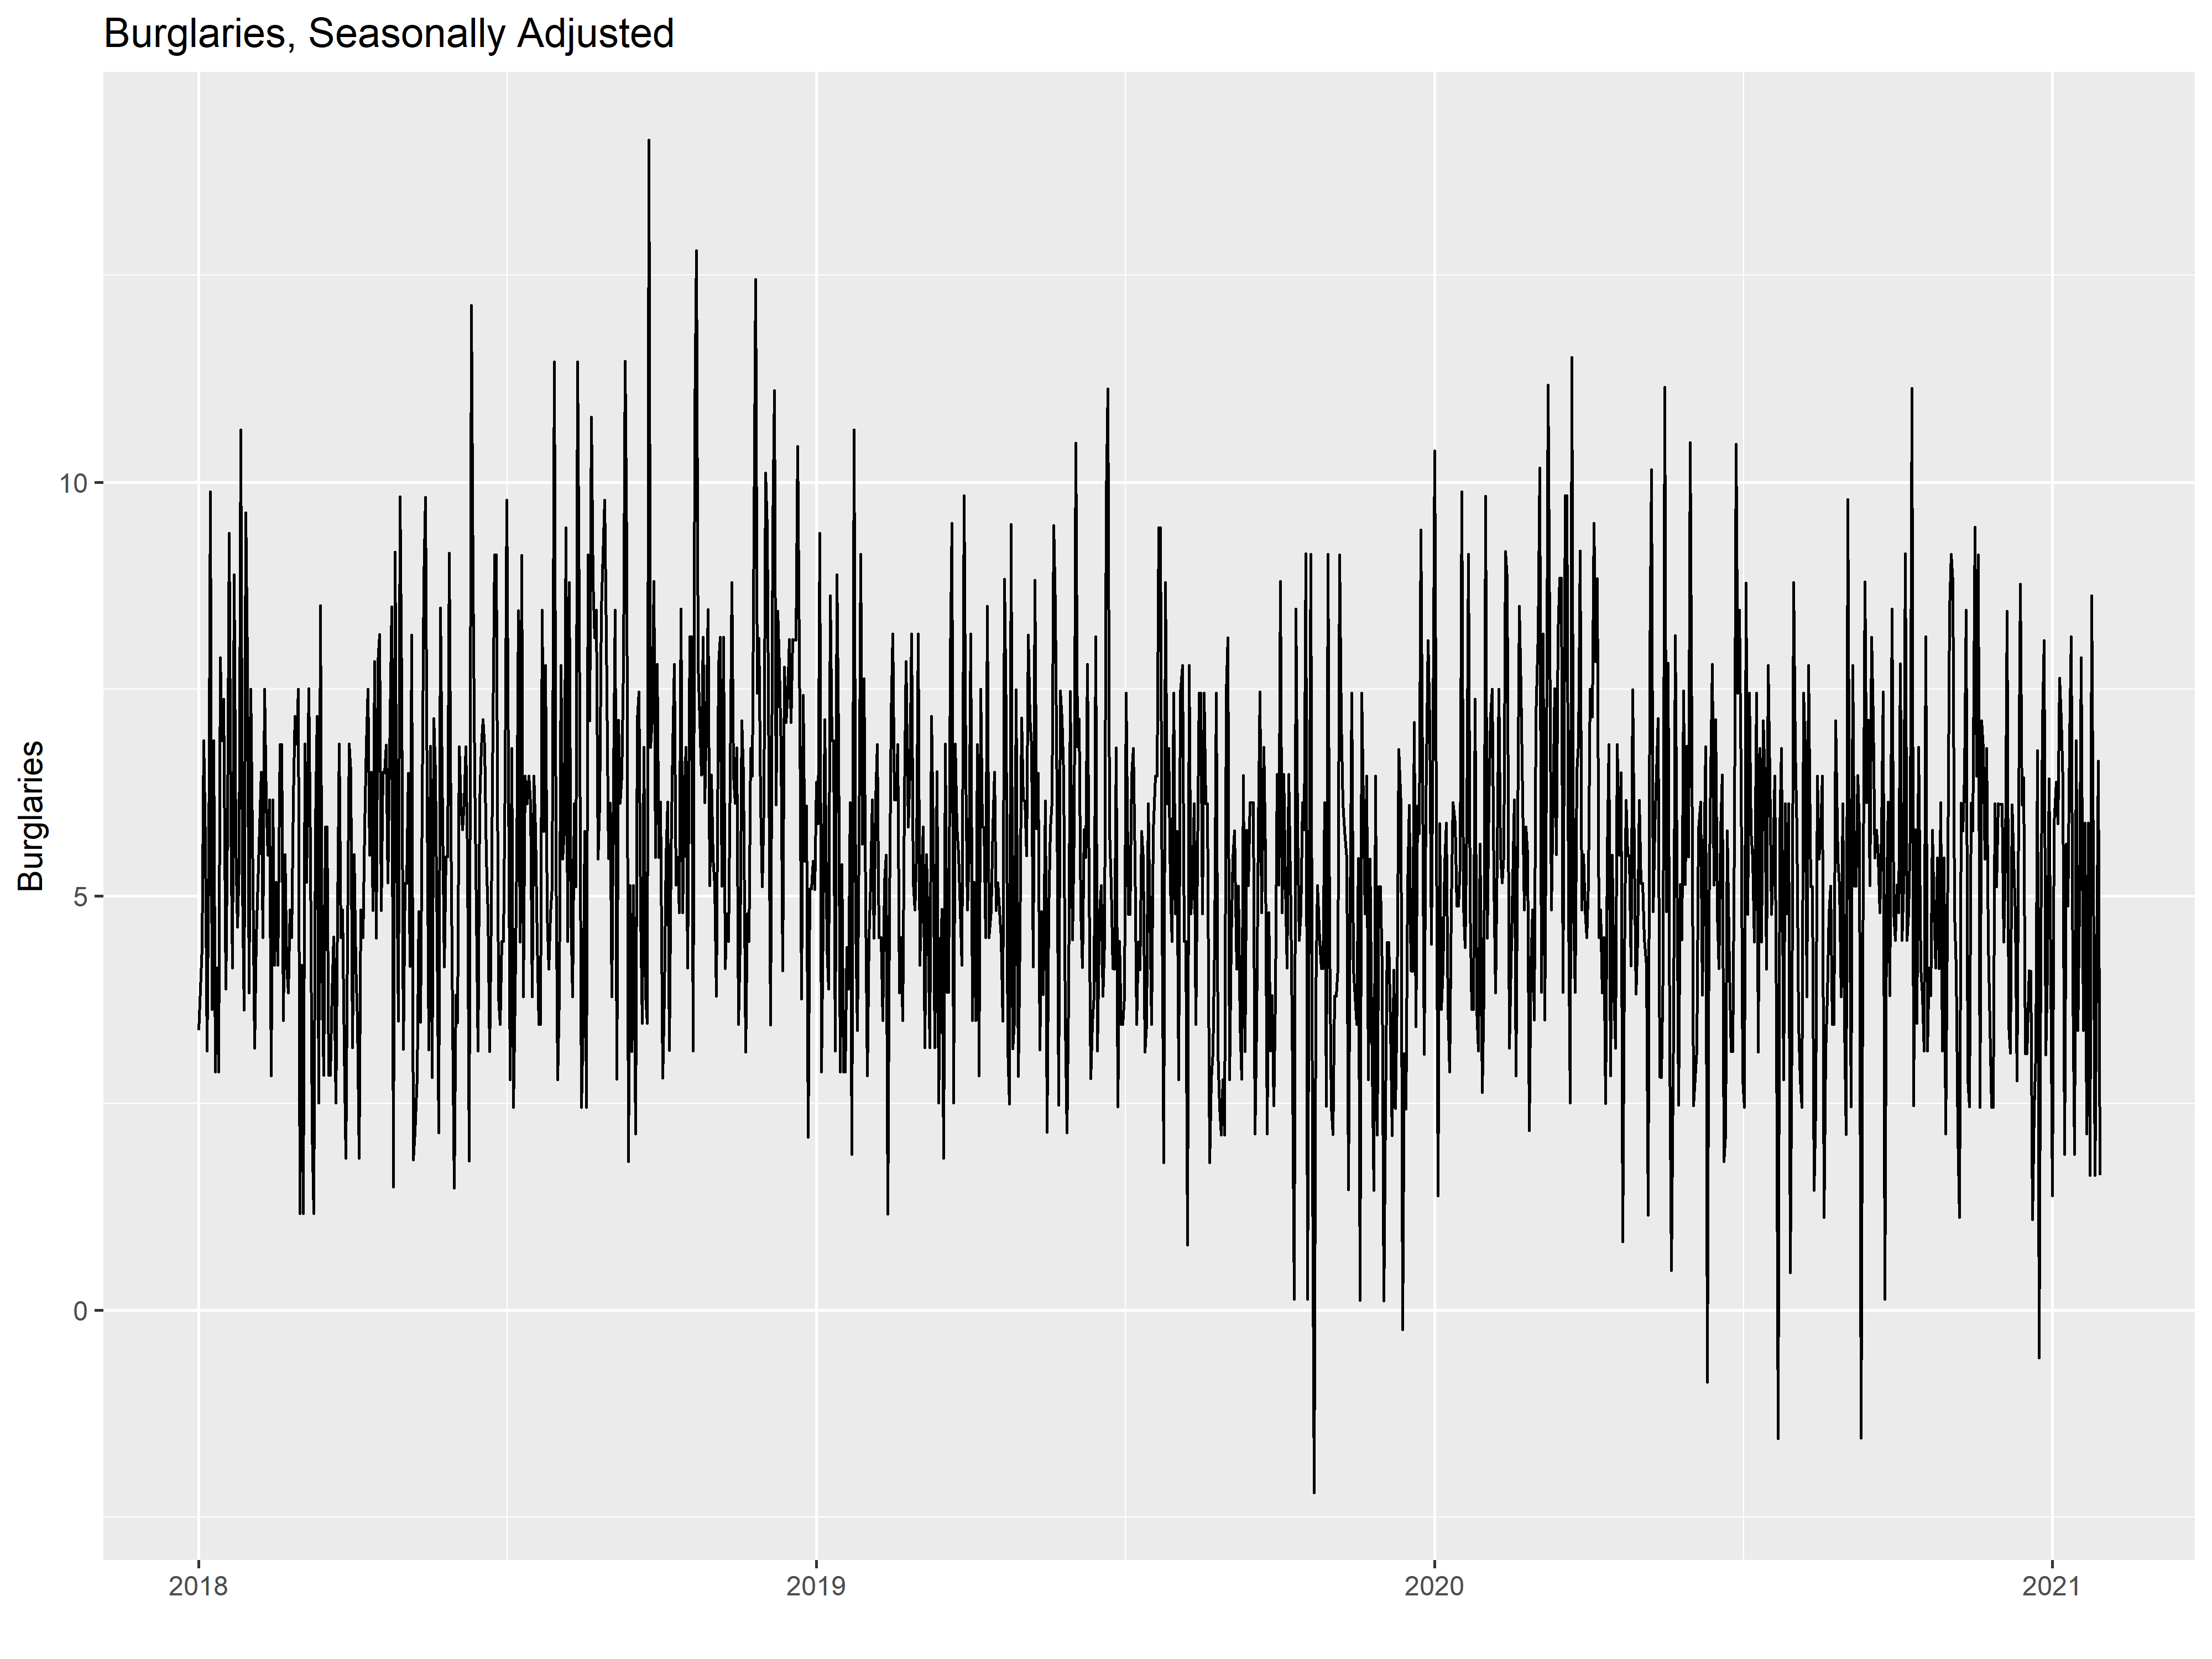
\includegraphics[width=\textwidth]{./figures/plot.burglaries_seasonally_adjusted-1} \end{center}

\begin{center}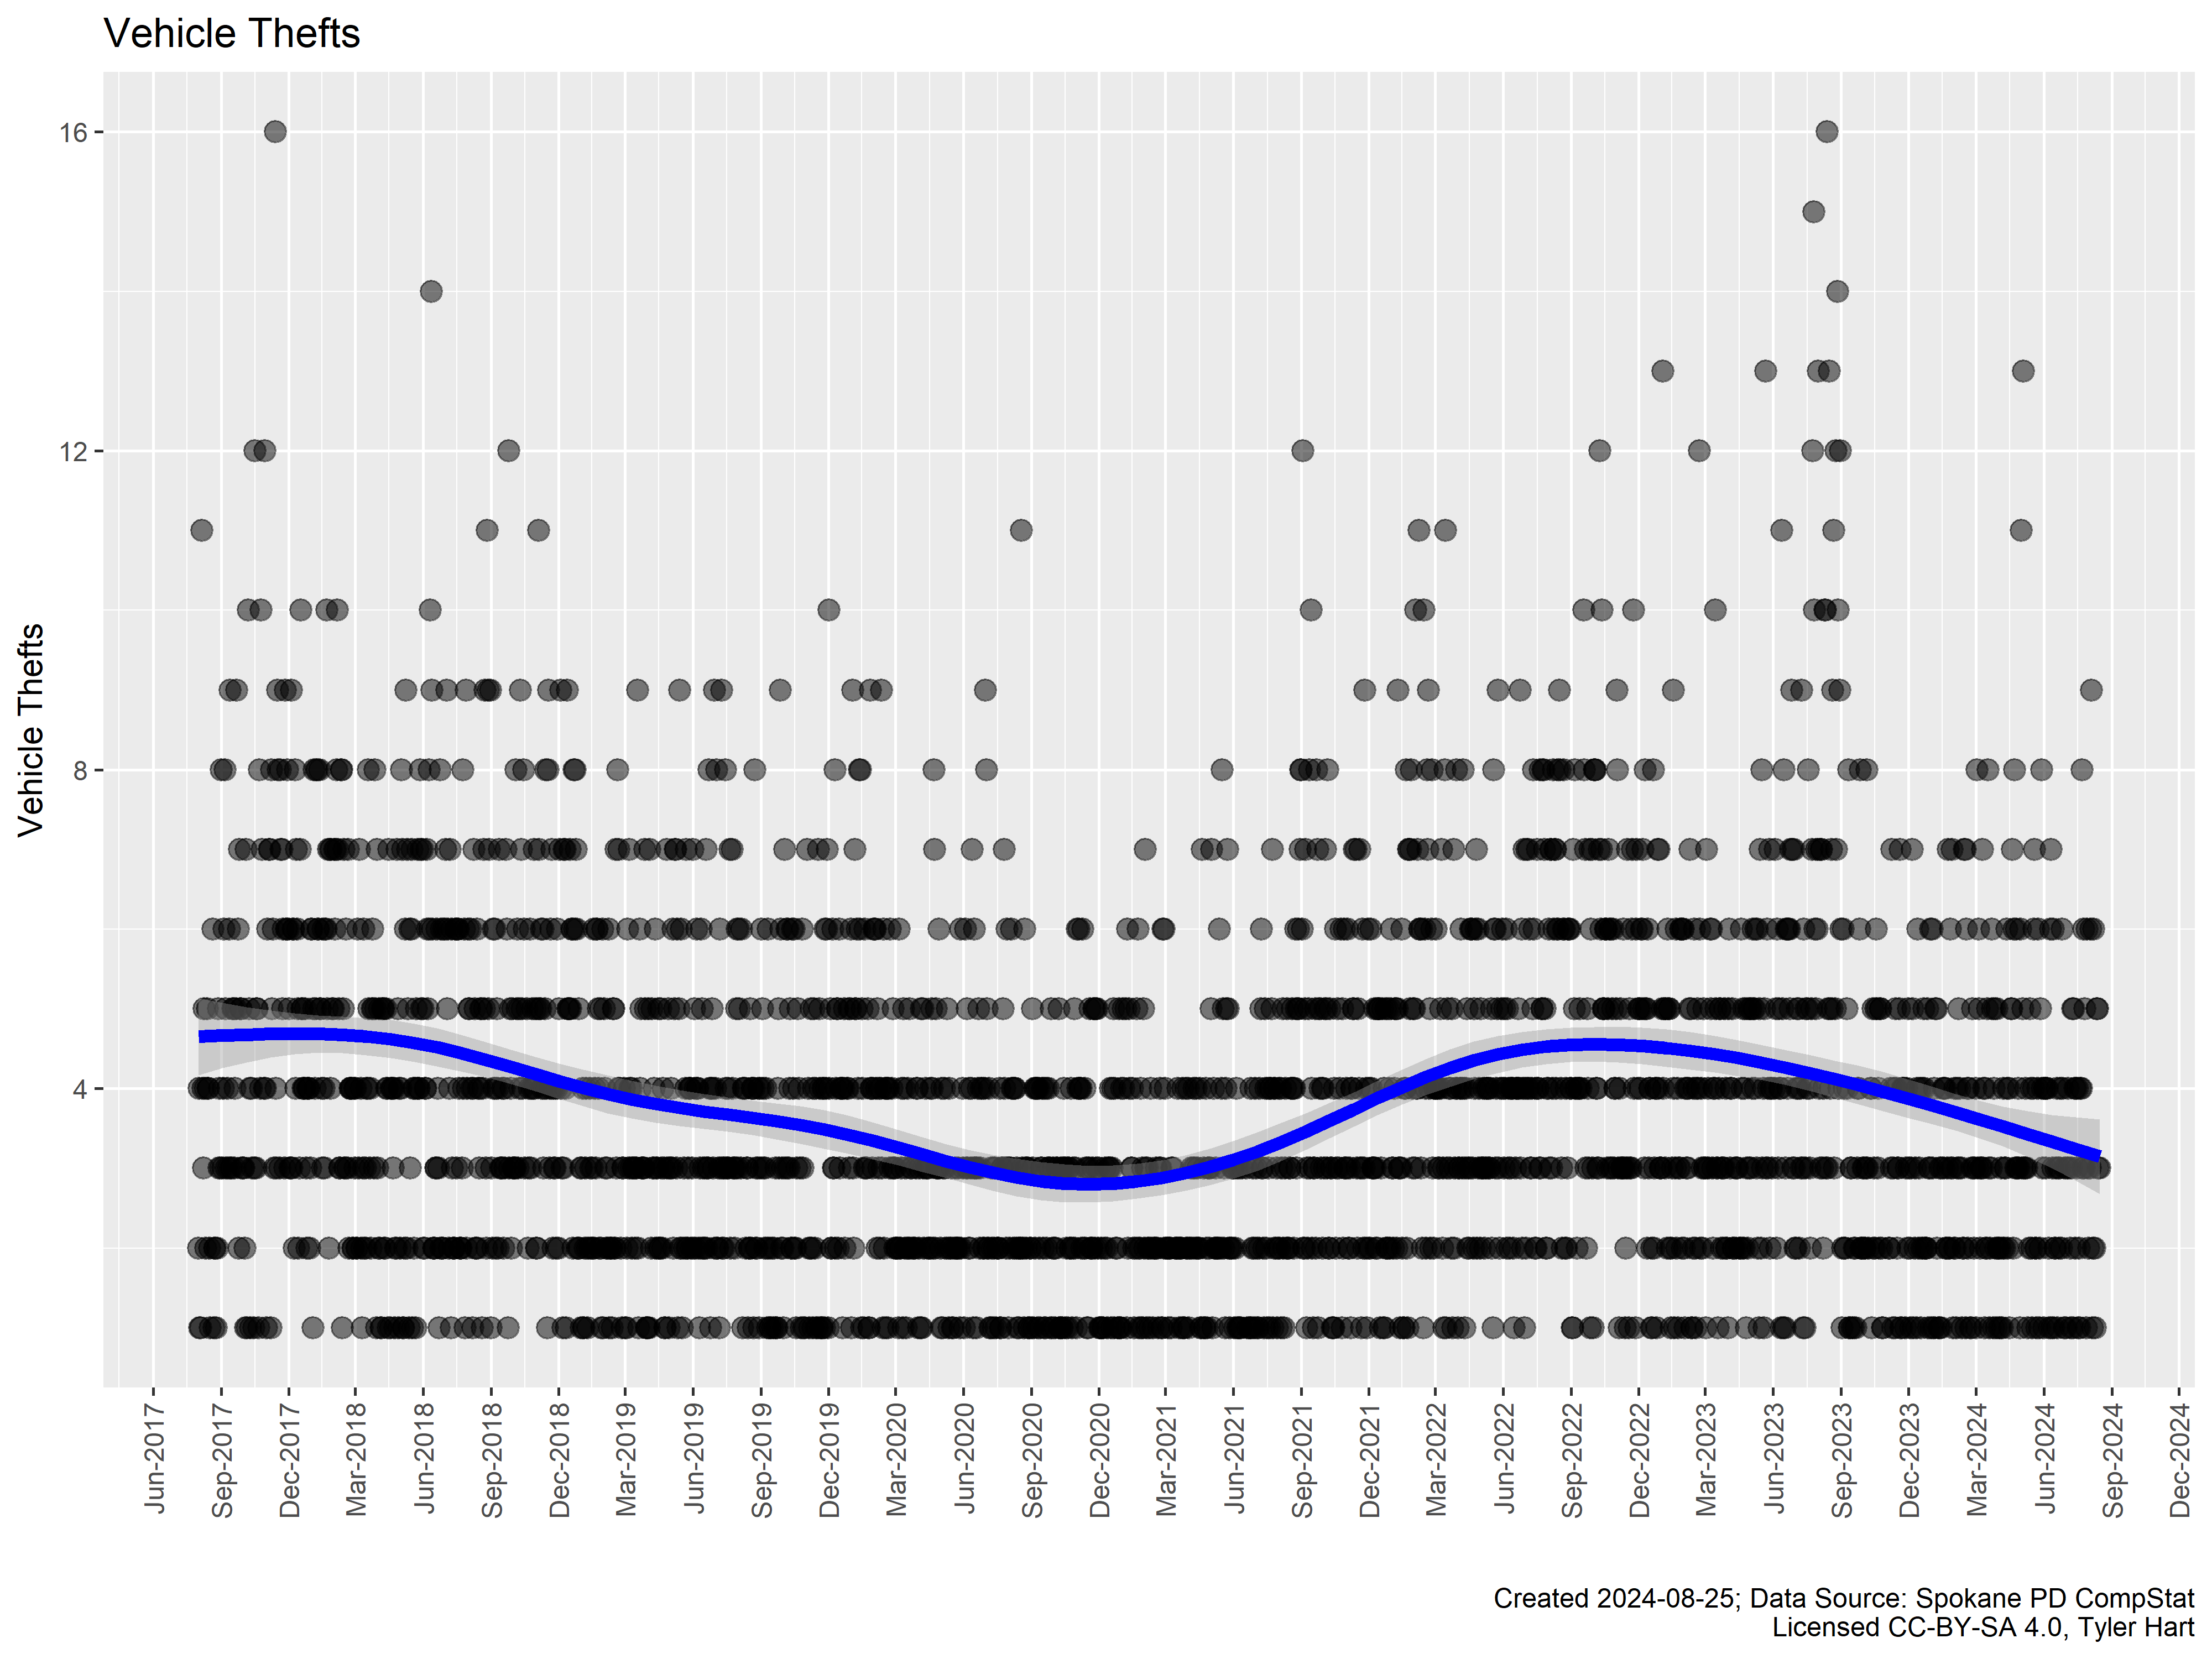
\includegraphics[width=\textwidth]{./figures/plot.tomv_over_time-1} \end{center}

\begin{center}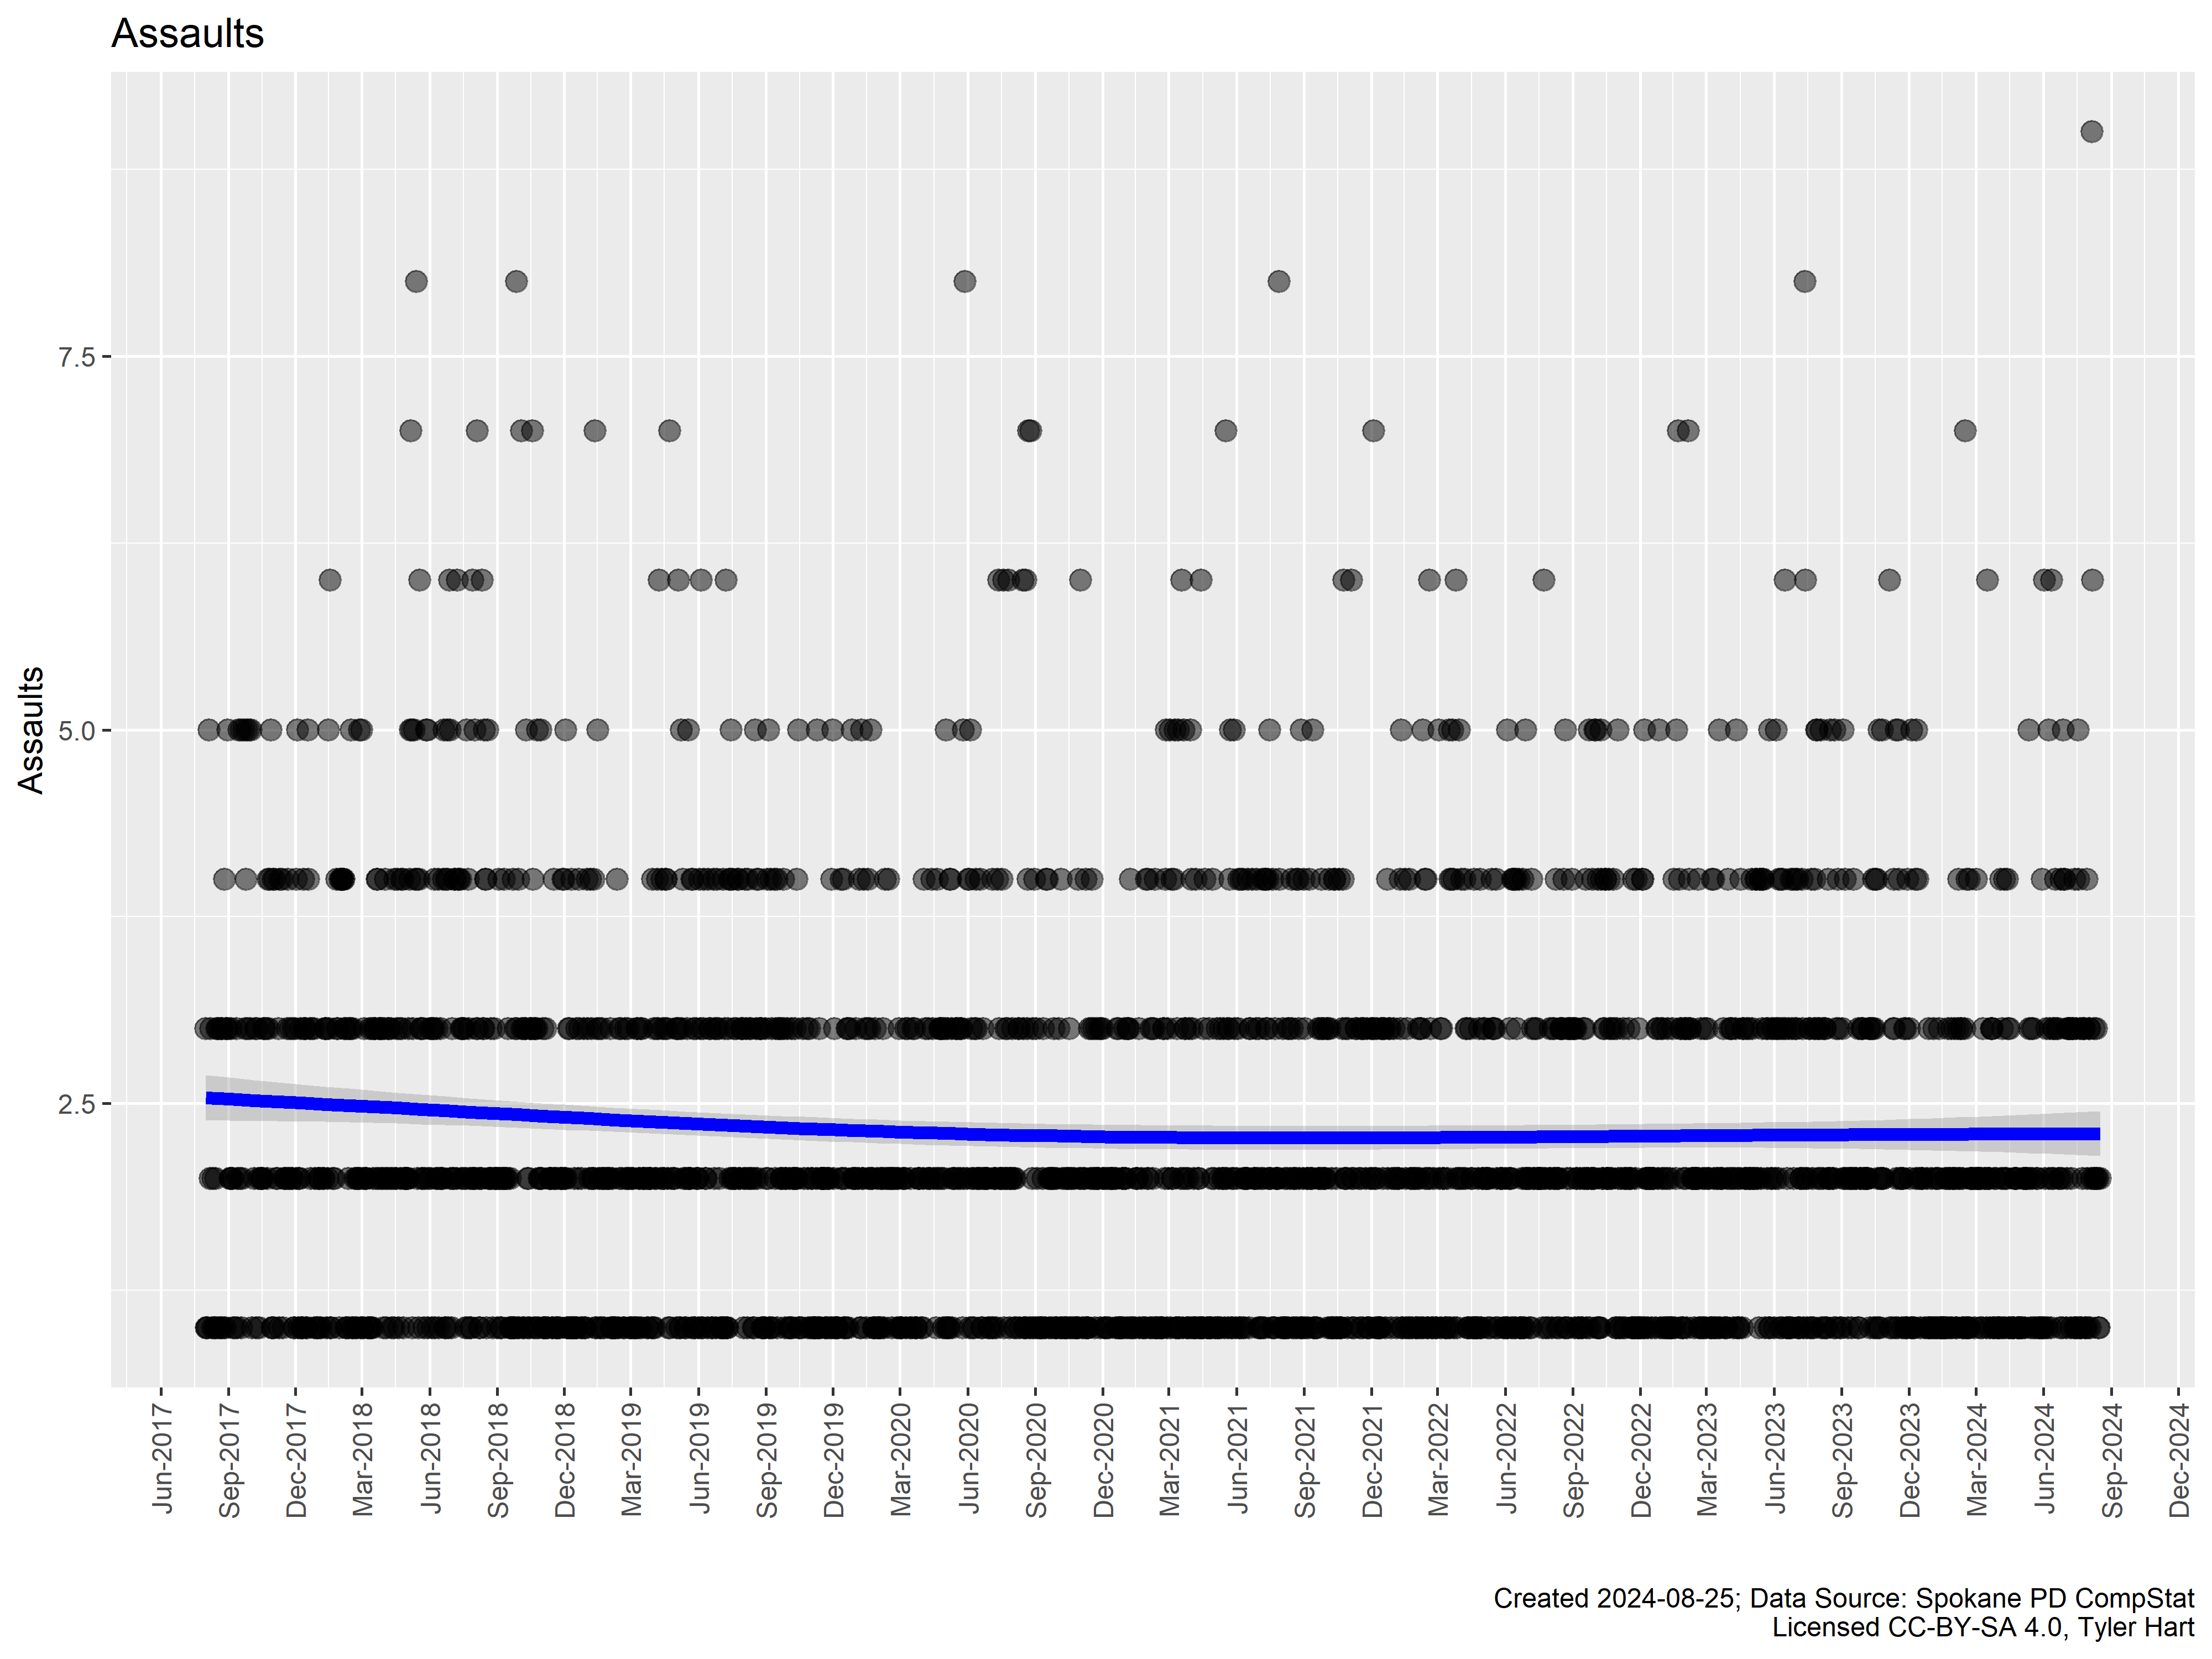
\includegraphics[width=\textwidth]{./figures/plot.assault_over_time-1} \end{center}

\begin{center}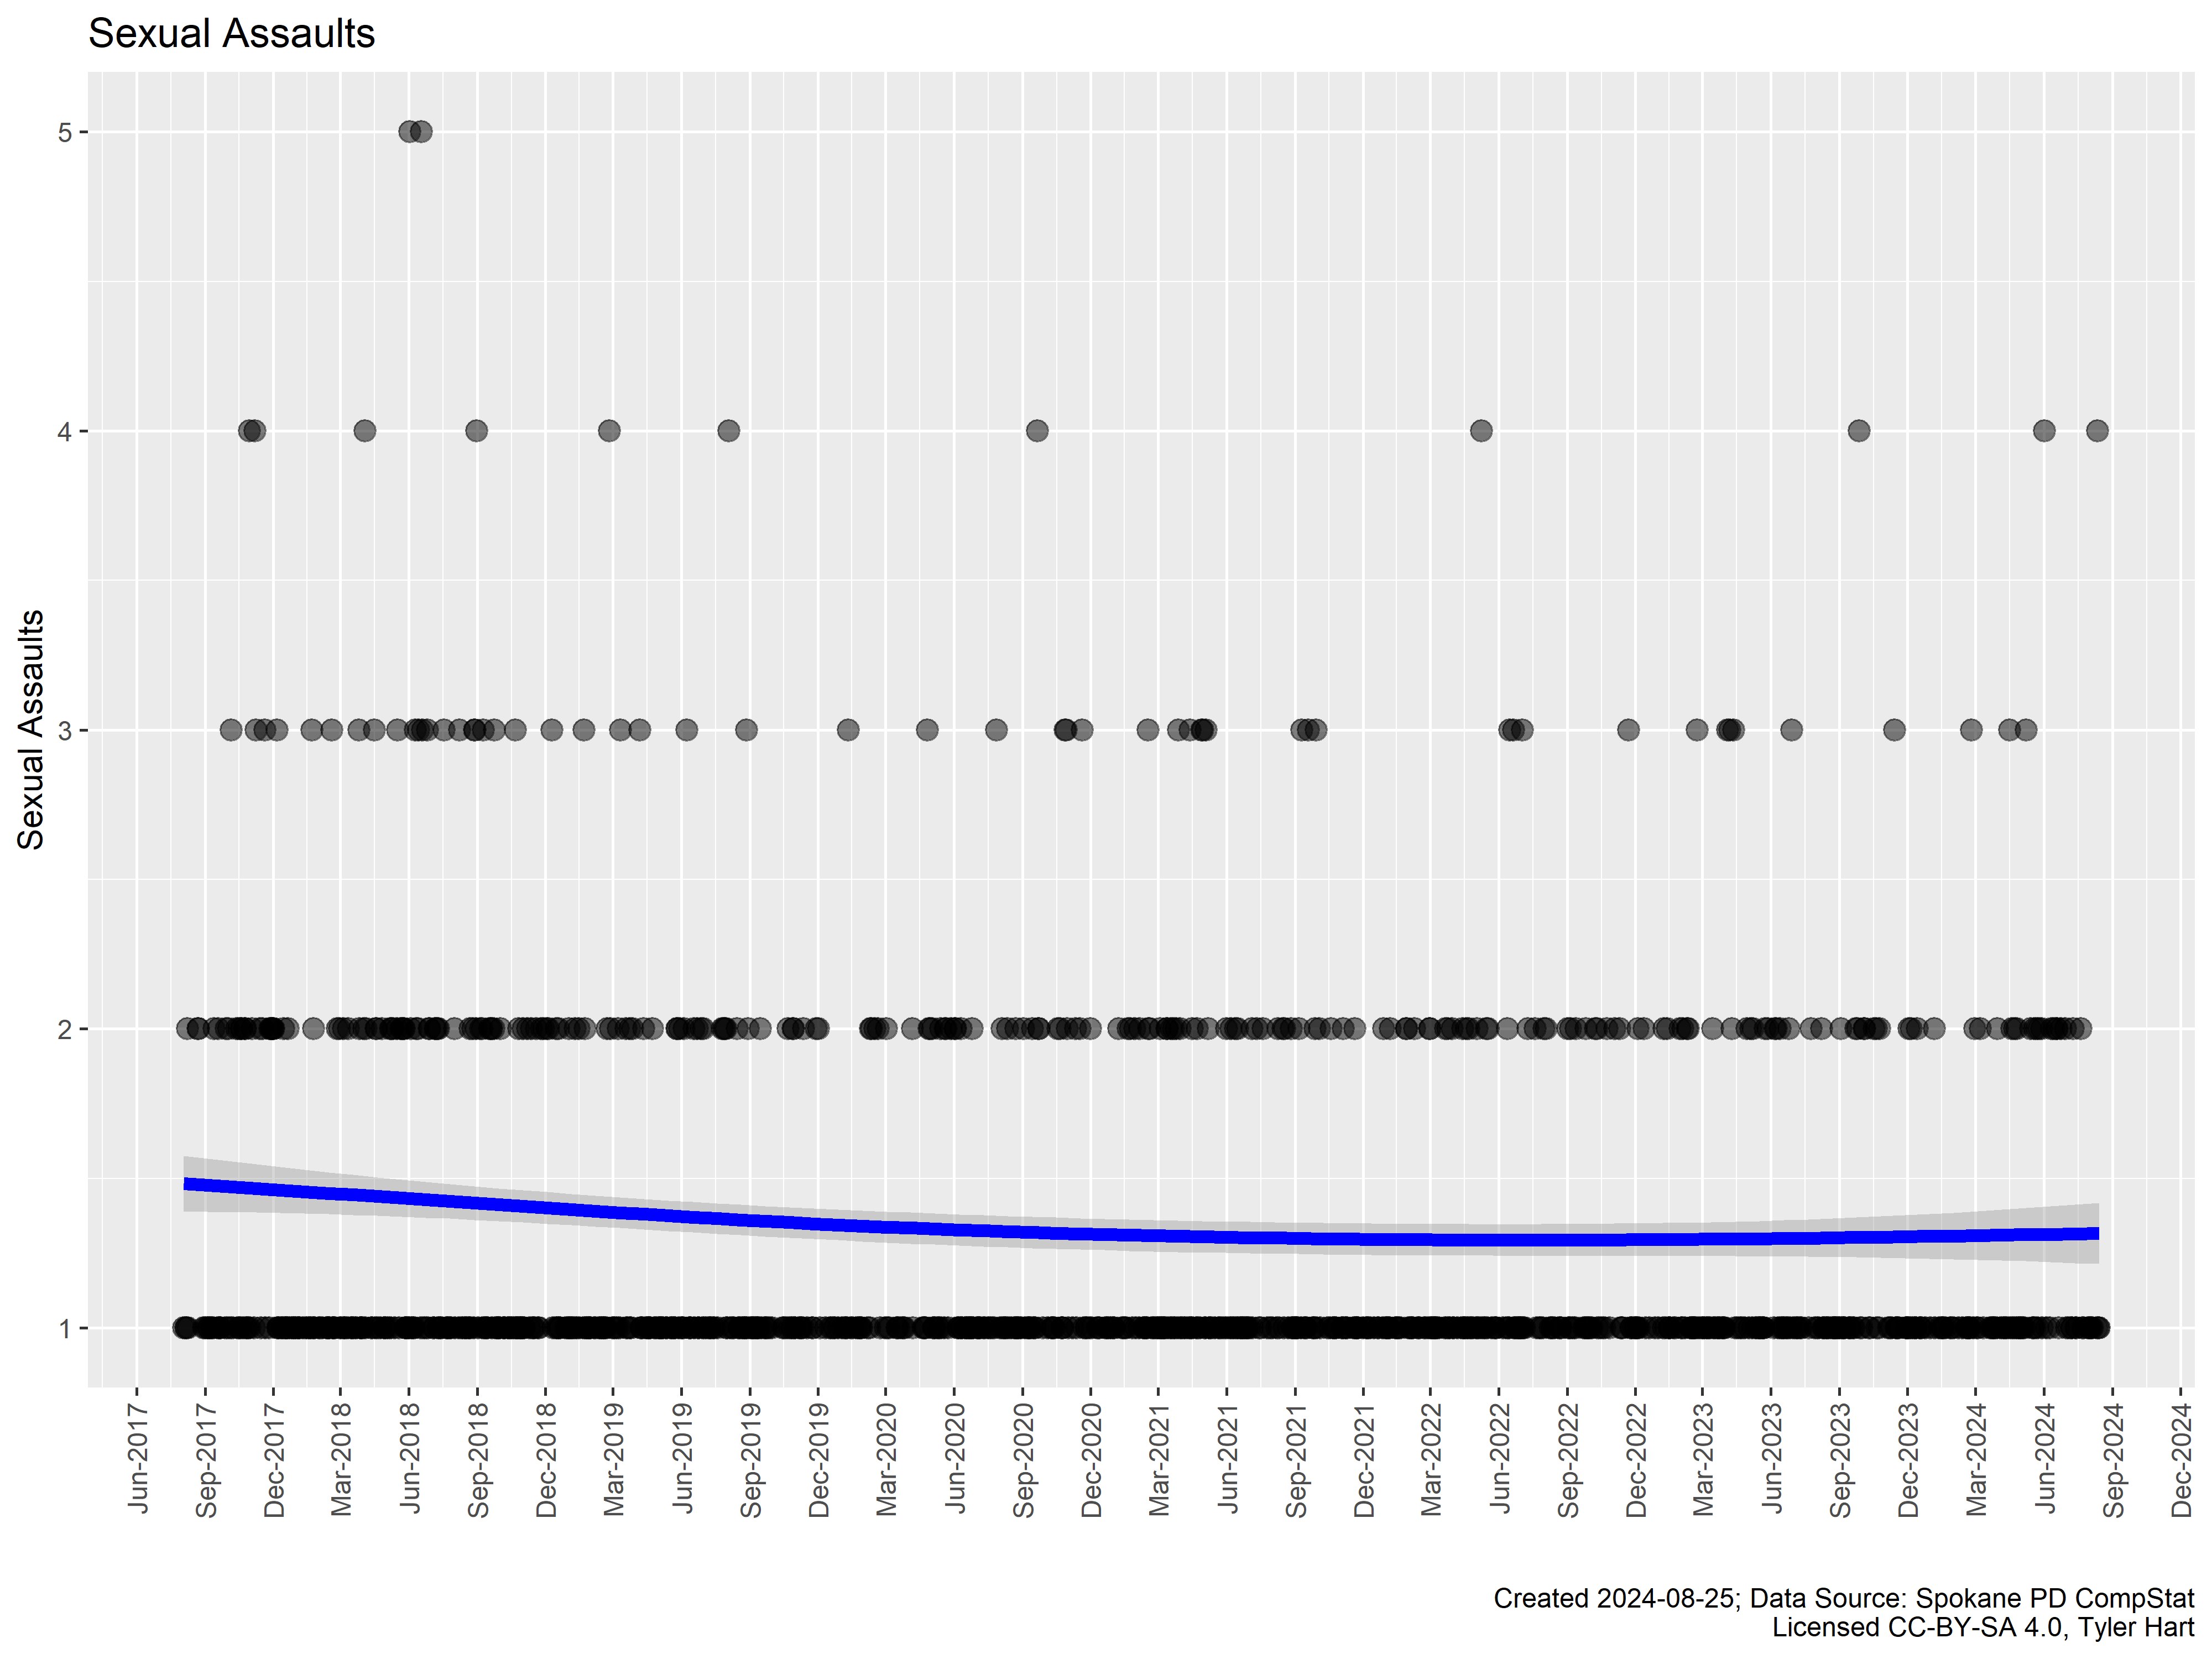
\includegraphics[width=\textwidth]{./figures/plot.rape_over_time-1} \end{center}

\hypertarget{police-districts}{%
\section{Police Districts}\label{police-districts}}

Spokane has a total of eight police districts. Those eight are divided
evenly between two main groups, the North and South Police Service
Areas. The Spokane River separates the two service areas, with Division
St.~and other major thoroughfares serving as boundaries. Districts P1 -
P4 are north of the Spokane River. Districts P5 - P8 are south of the
river. Some incidents in the CompStat reports are listed as ``OTH'',
meaning ``Other''.

\begin{itemize}
\tightlist
\item
  P1: Northwest District
\item
  P2: Central District
\item
  P3: Neva-Wood District
\item
  P4: Northeast District
\item
  P5: South Central District
\item
  P6: Southeast District
\item
  P7: Southwest District
\item
  P8: Downtown District
\item
  OTH: Other District
\end{itemize}

\begin{center}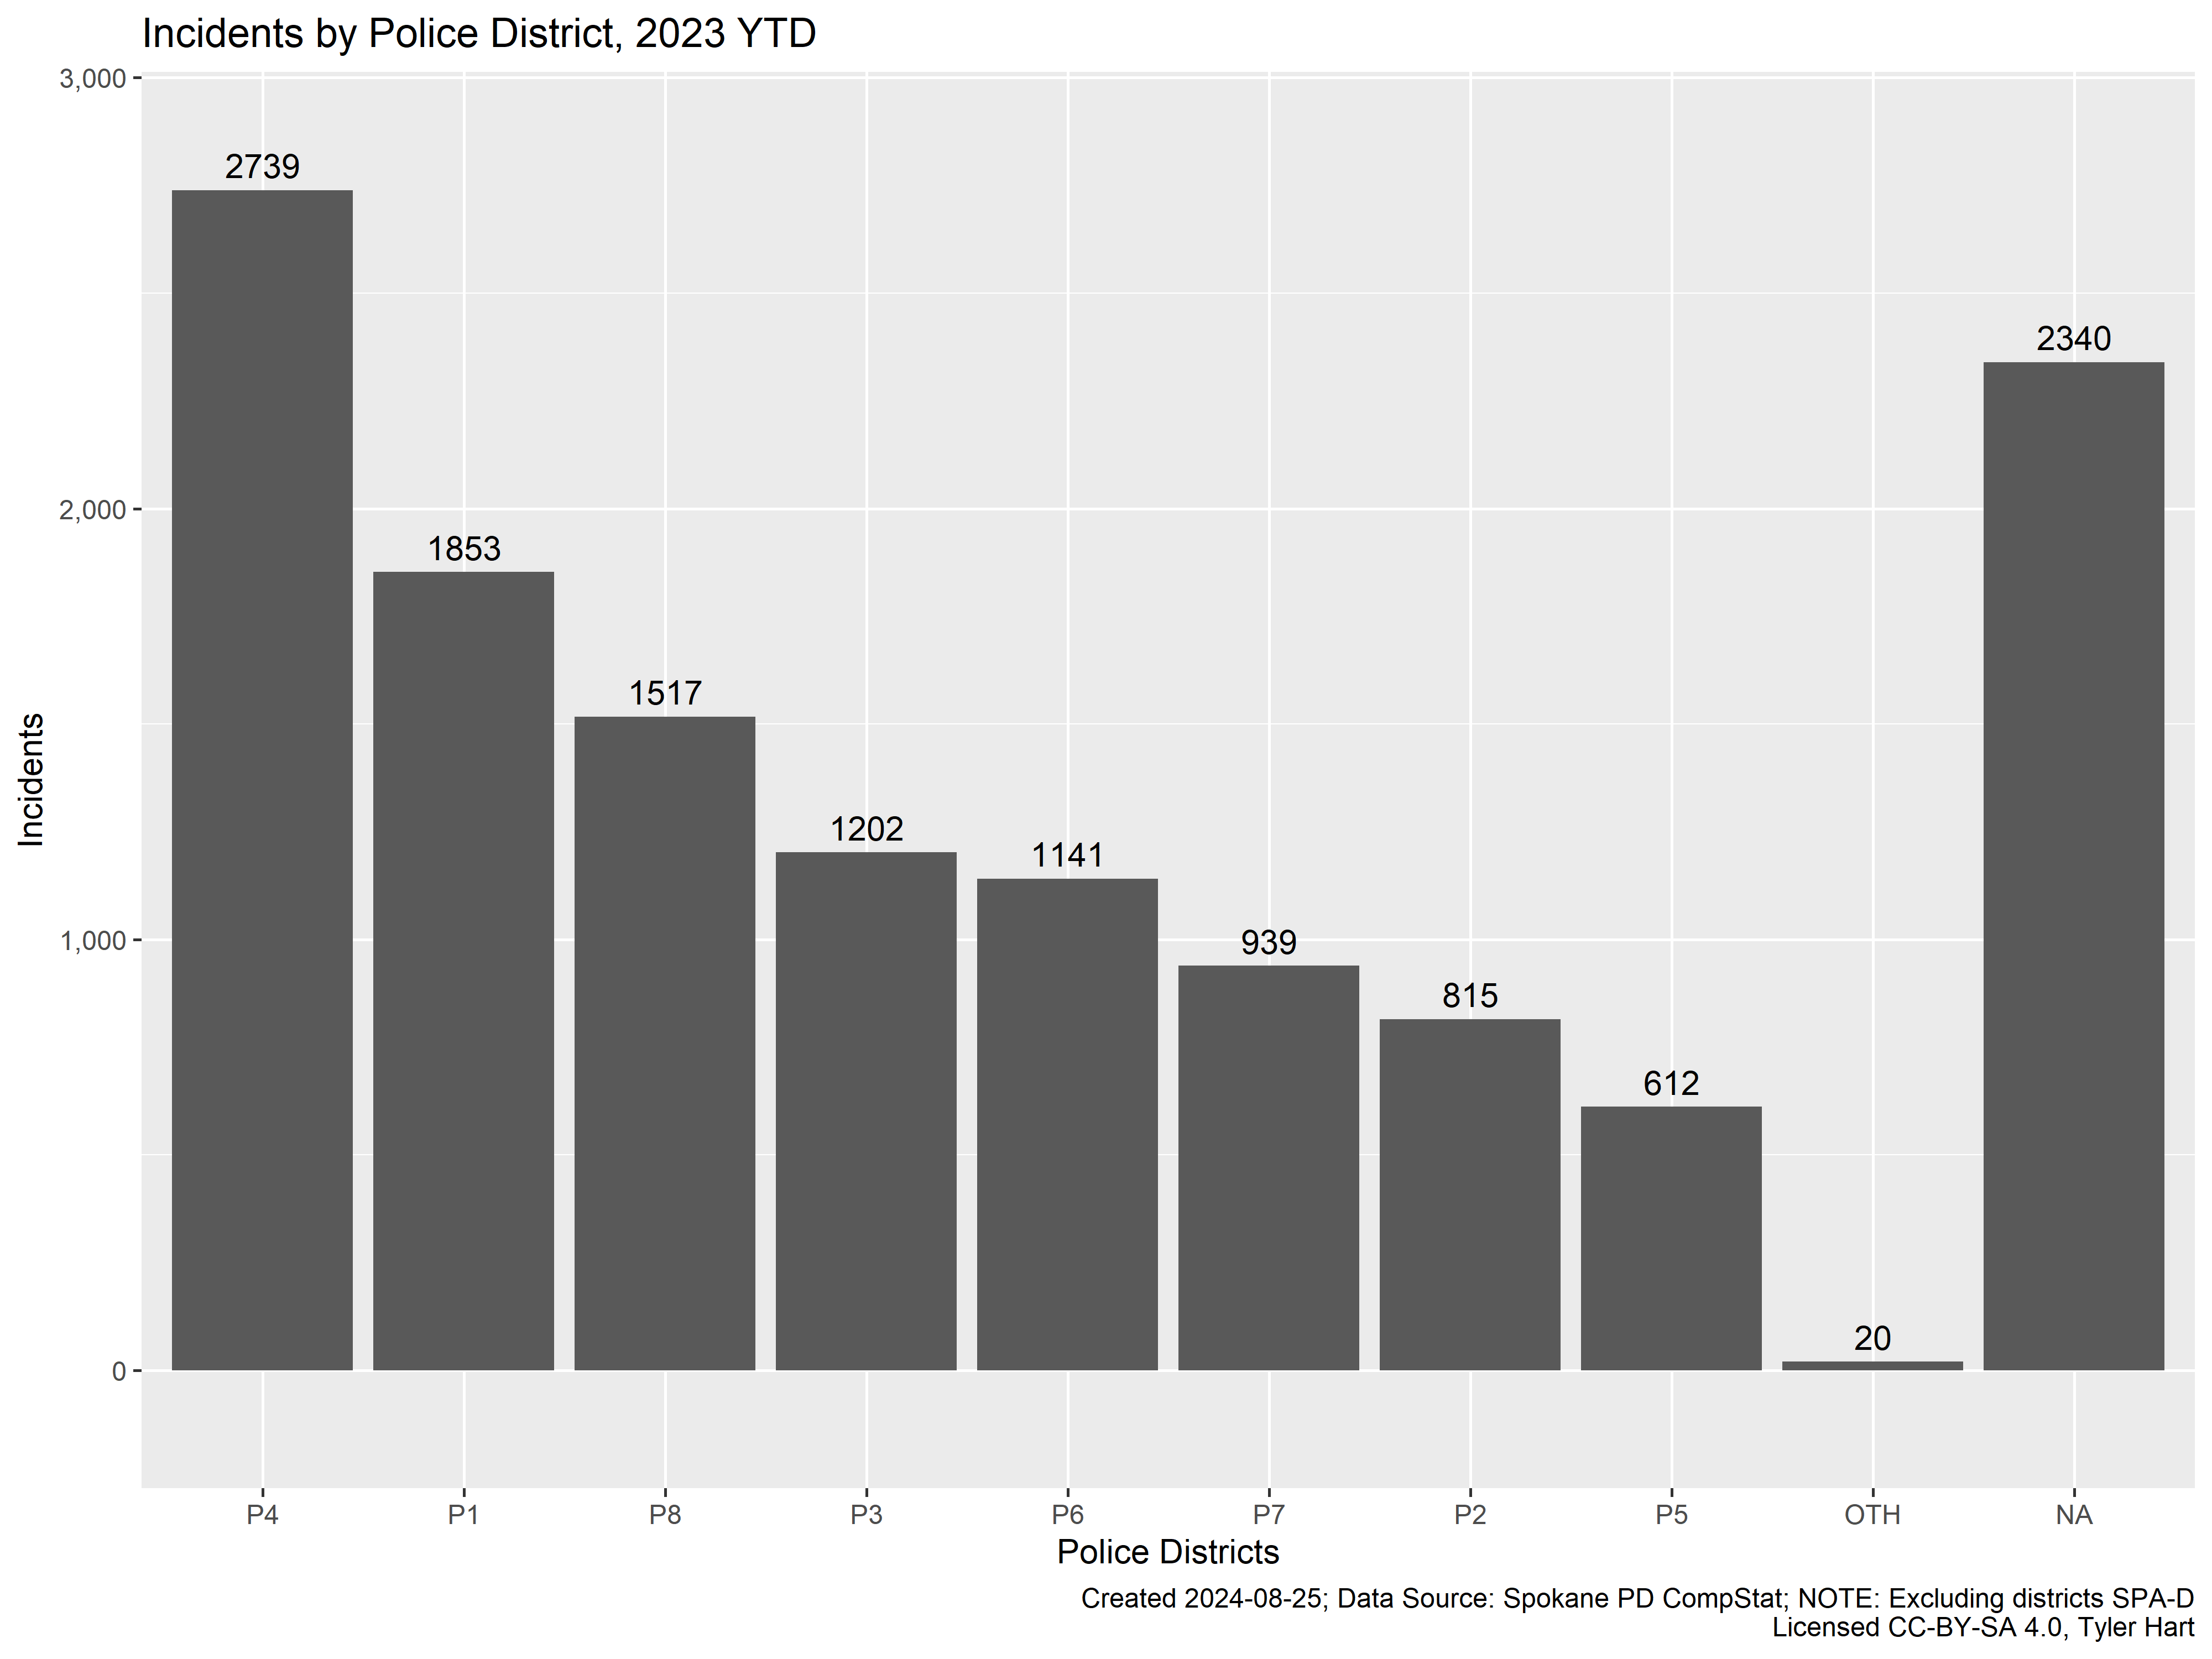
\includegraphics[width=\textwidth]{./figures/plot.ytd_offenses_by_district-1} \end{center}

\begin{center}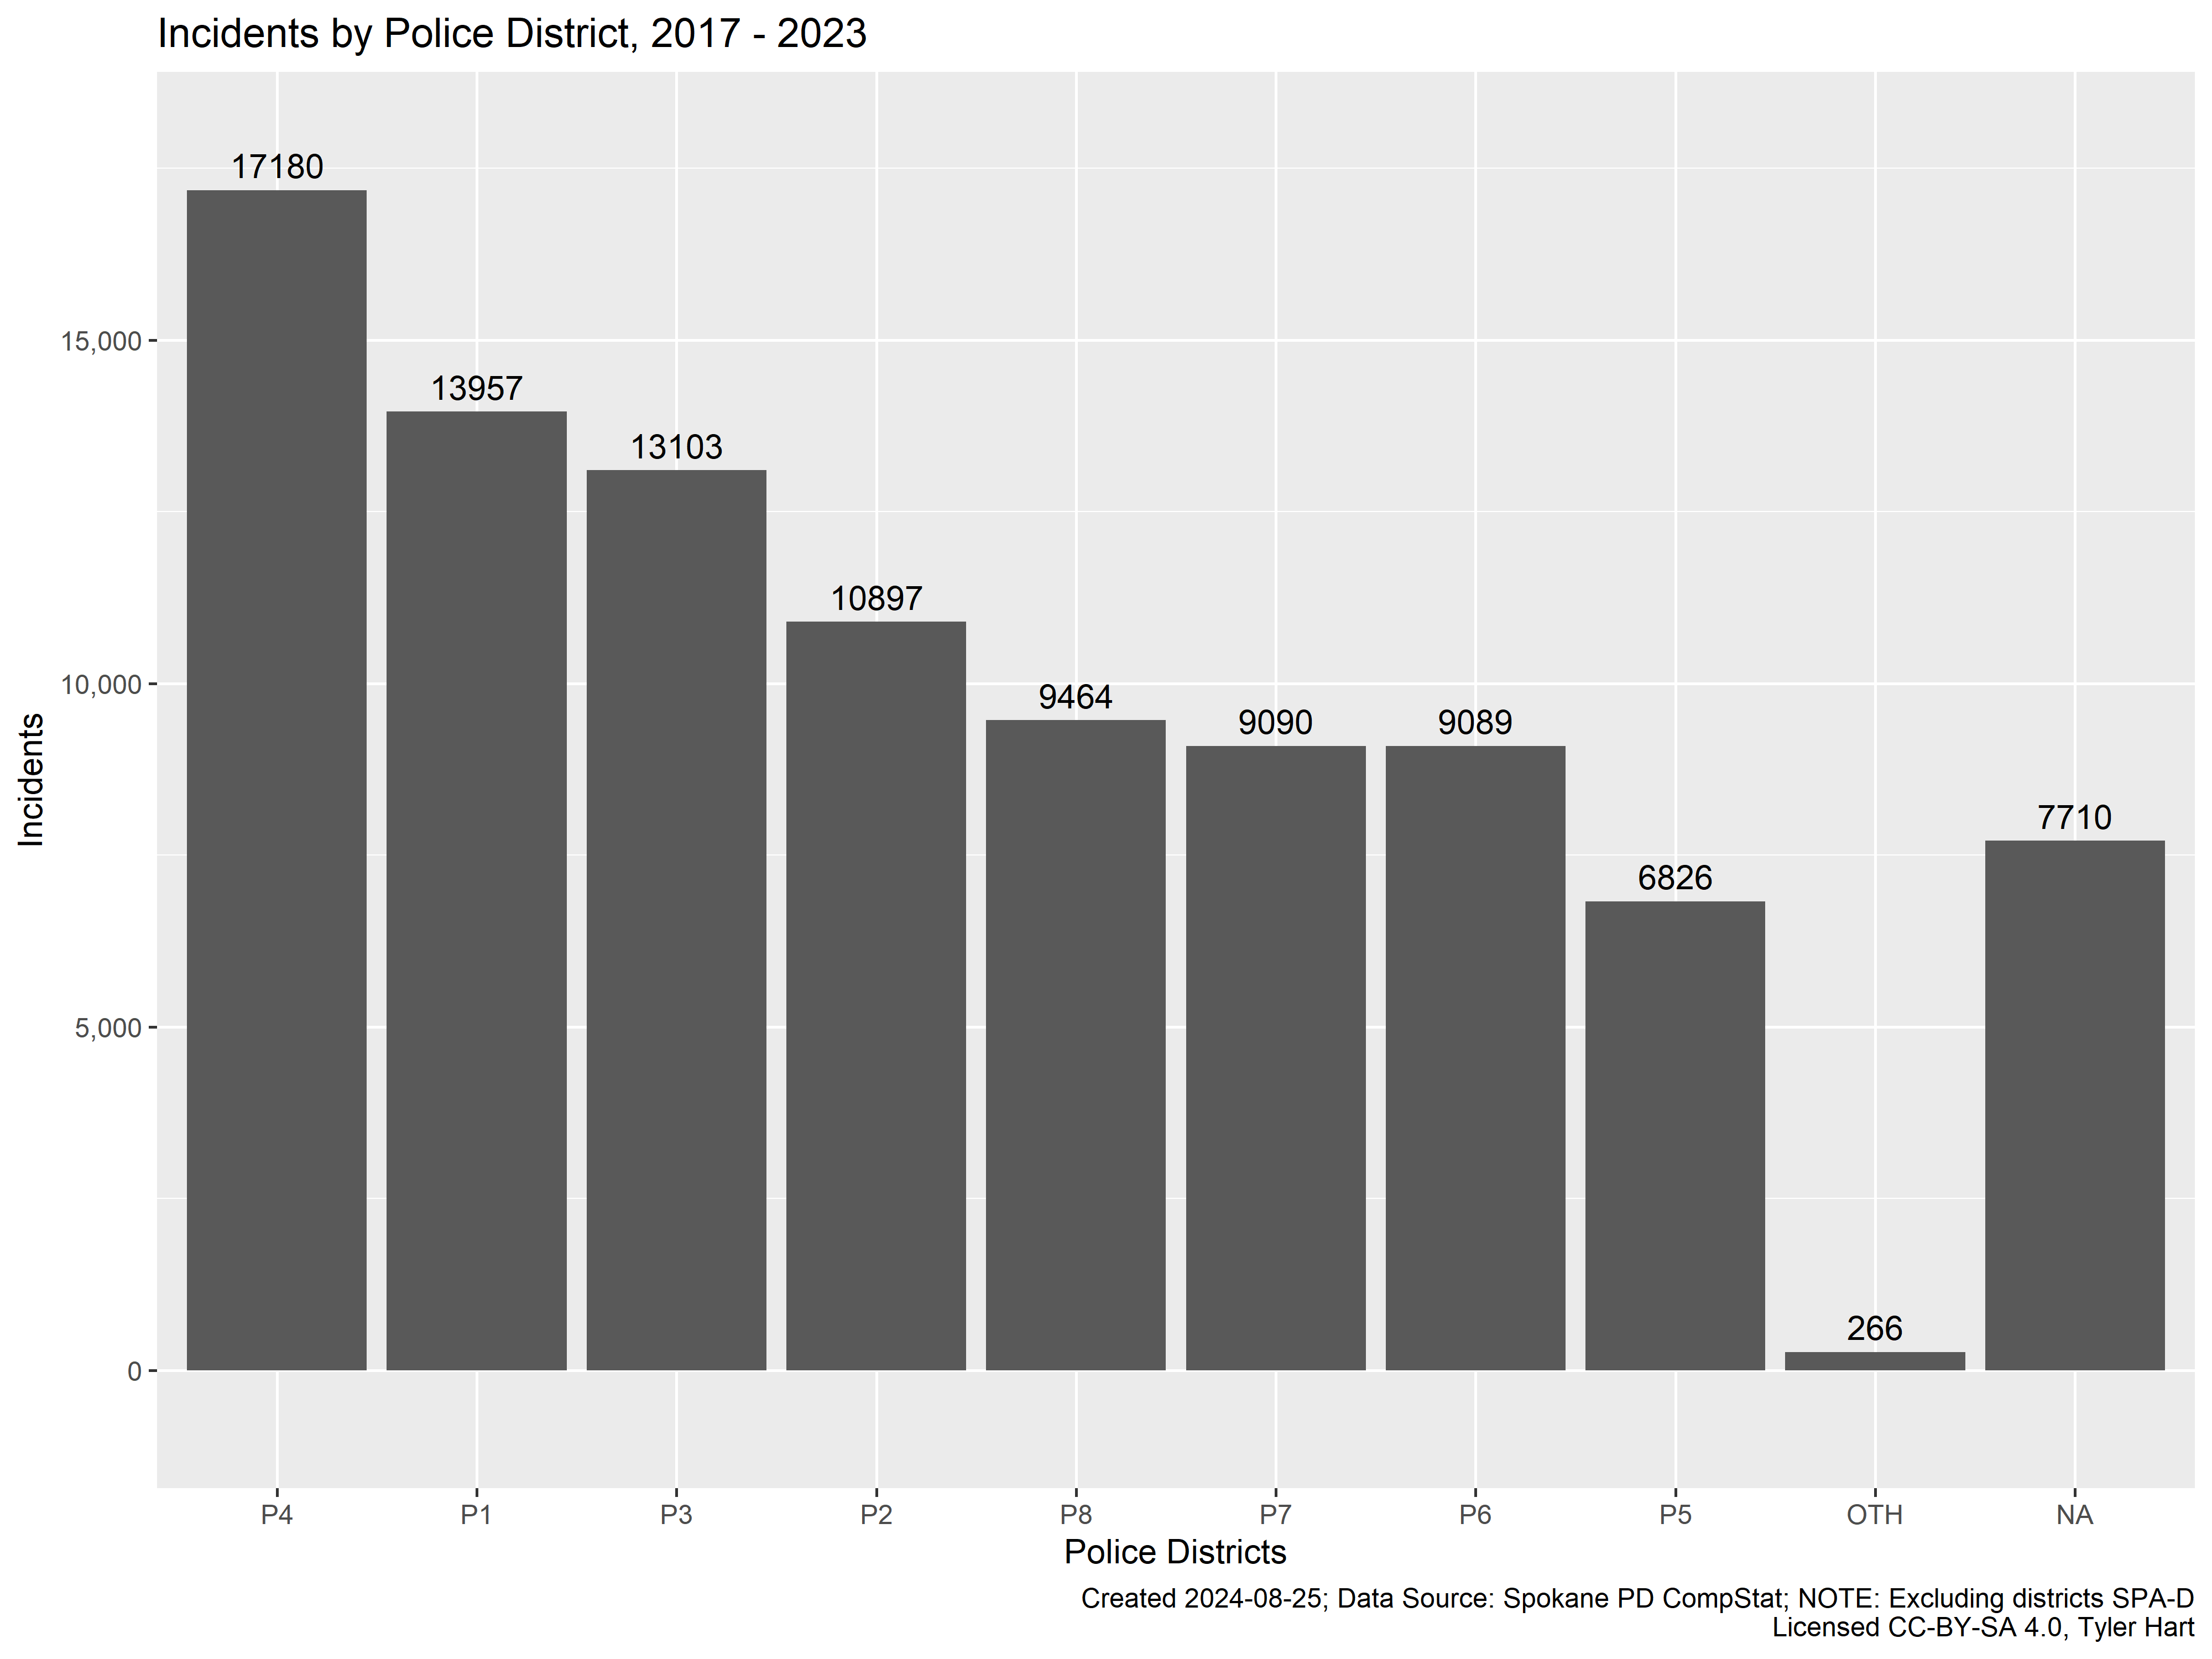
\includegraphics[width=\textwidth]{./figures/plot.total_offenses_by_district-1} \end{center}

\begin{center}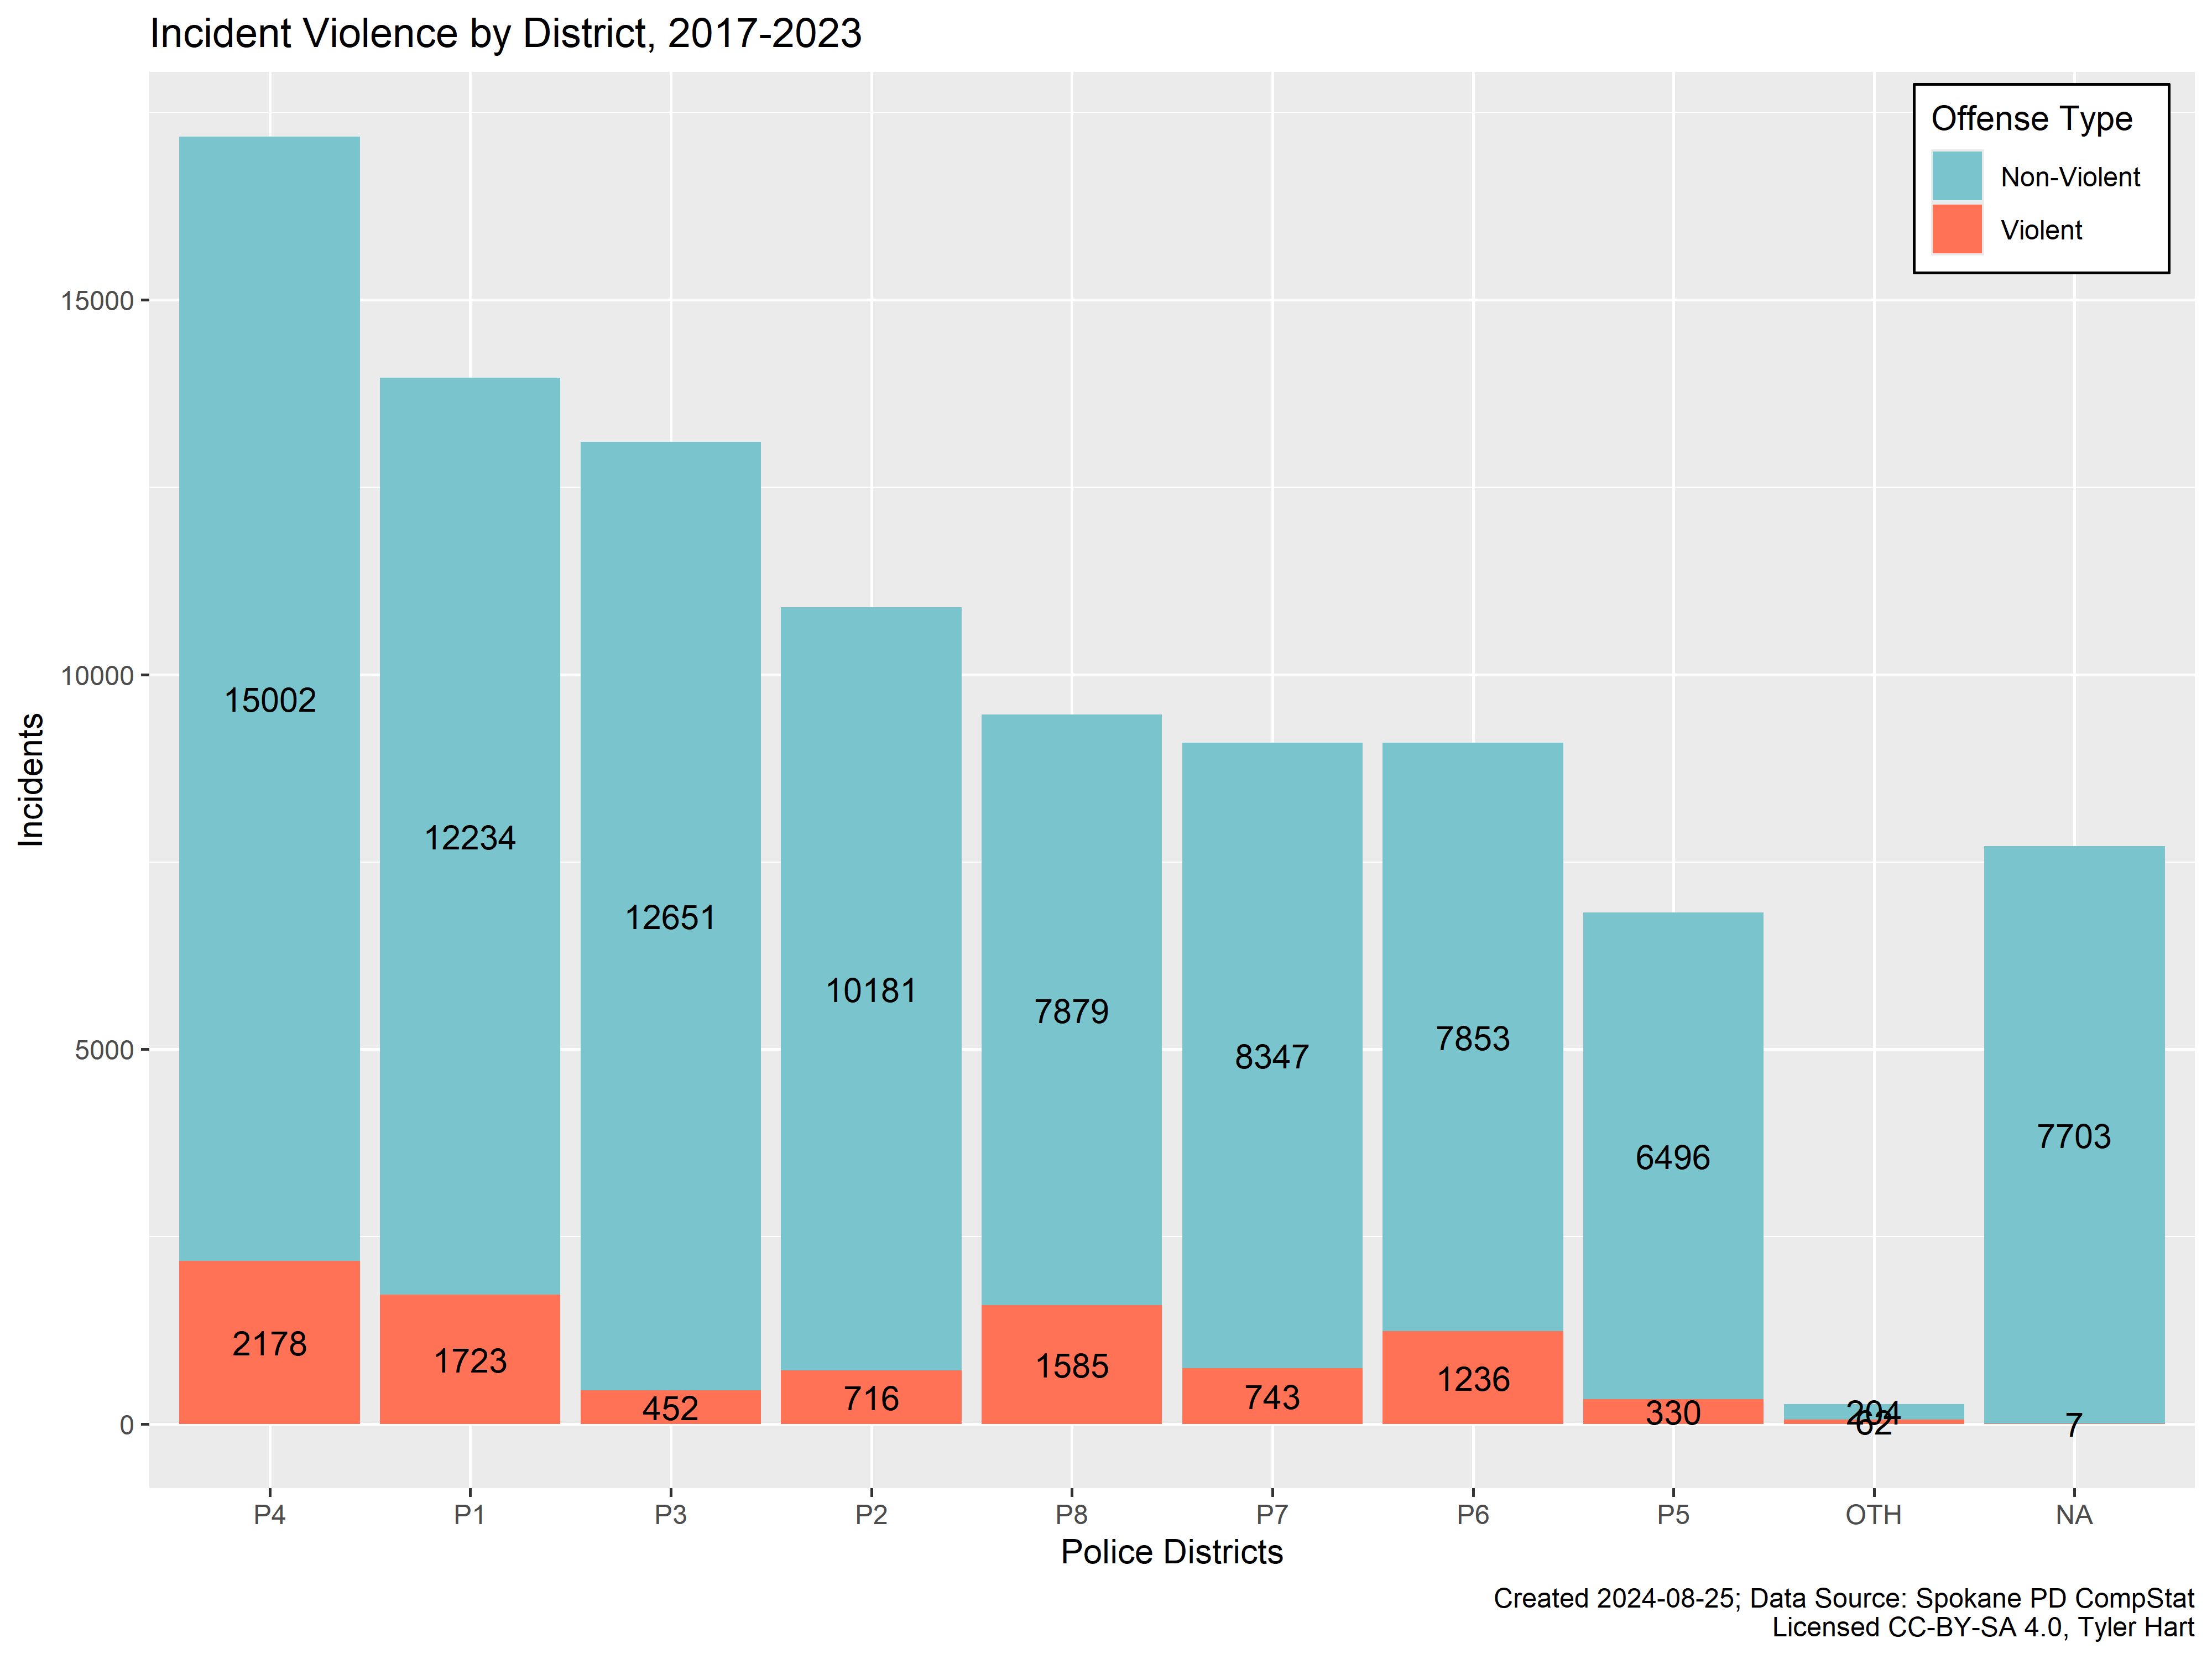
\includegraphics[width=\textwidth]{./figures/plot.total_offenses_by_violence_district-1} \end{center}

\begin{center}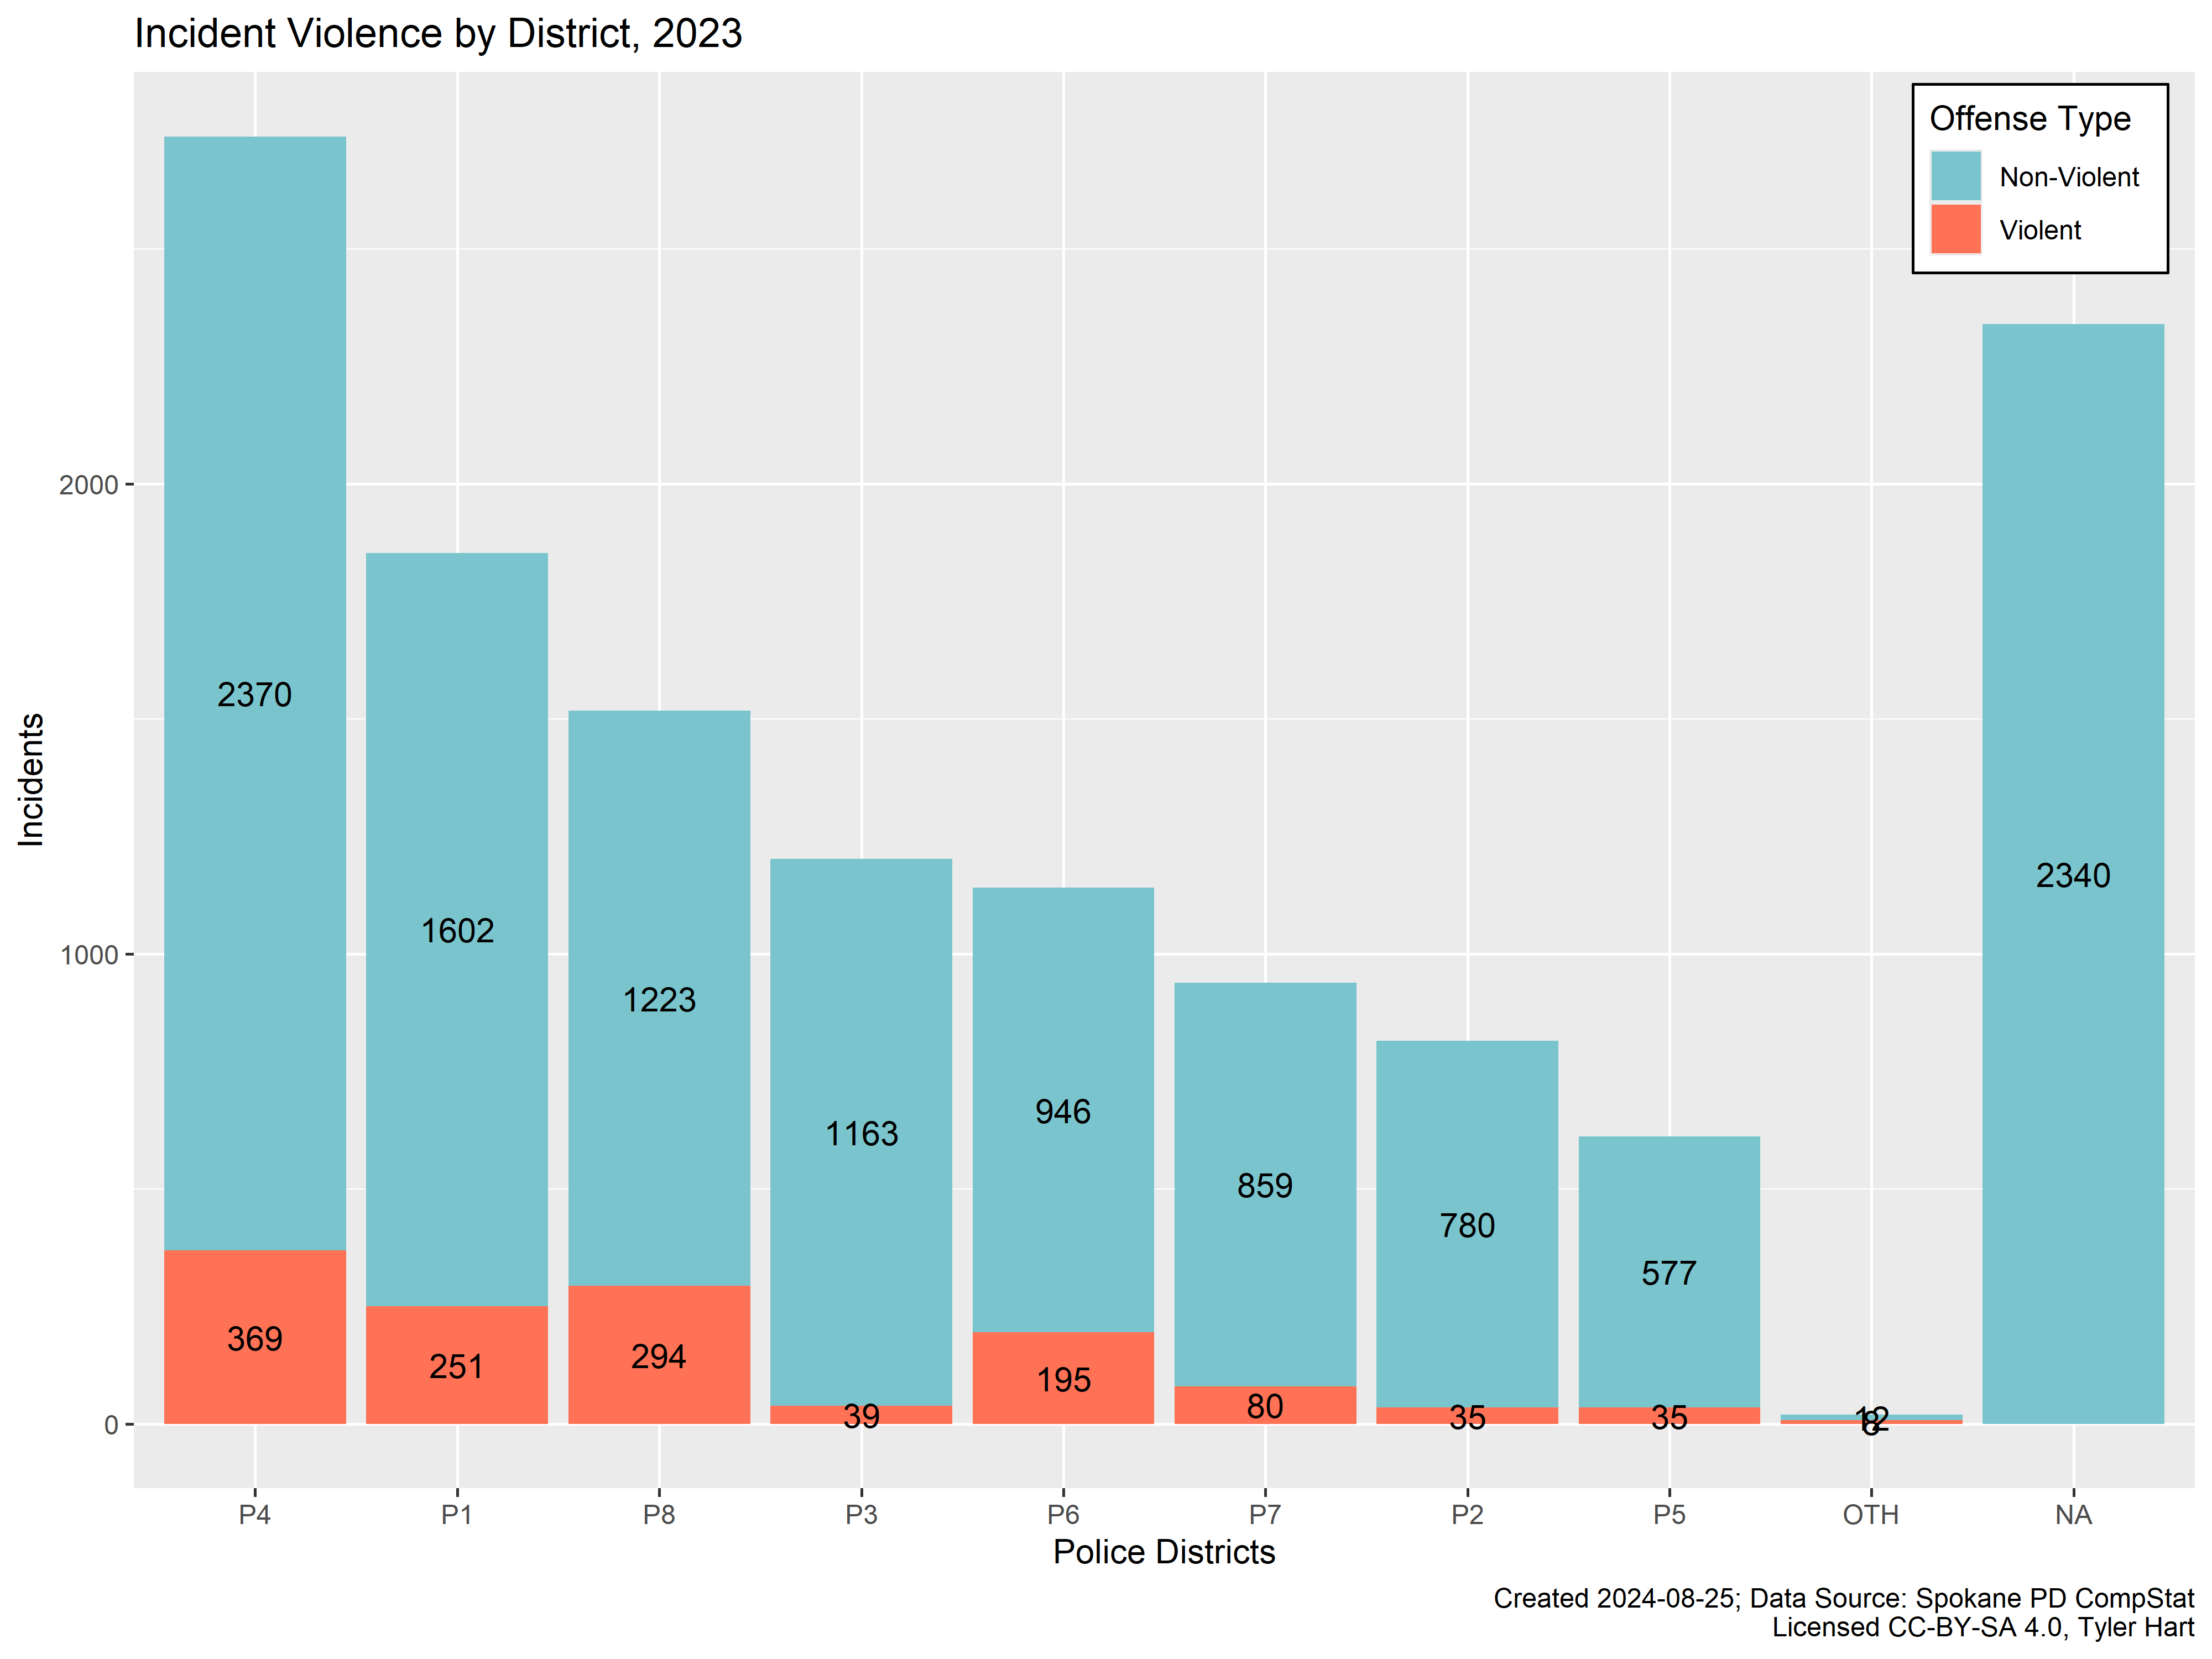
\includegraphics[width=\textwidth]{./figures/plot.ytd_offenses_by_violence_district-1} \end{center}

\hypertarget{north-south-districts}{%
\subsection{North, South Districts}\label{north-south-districts}}

\begin{center}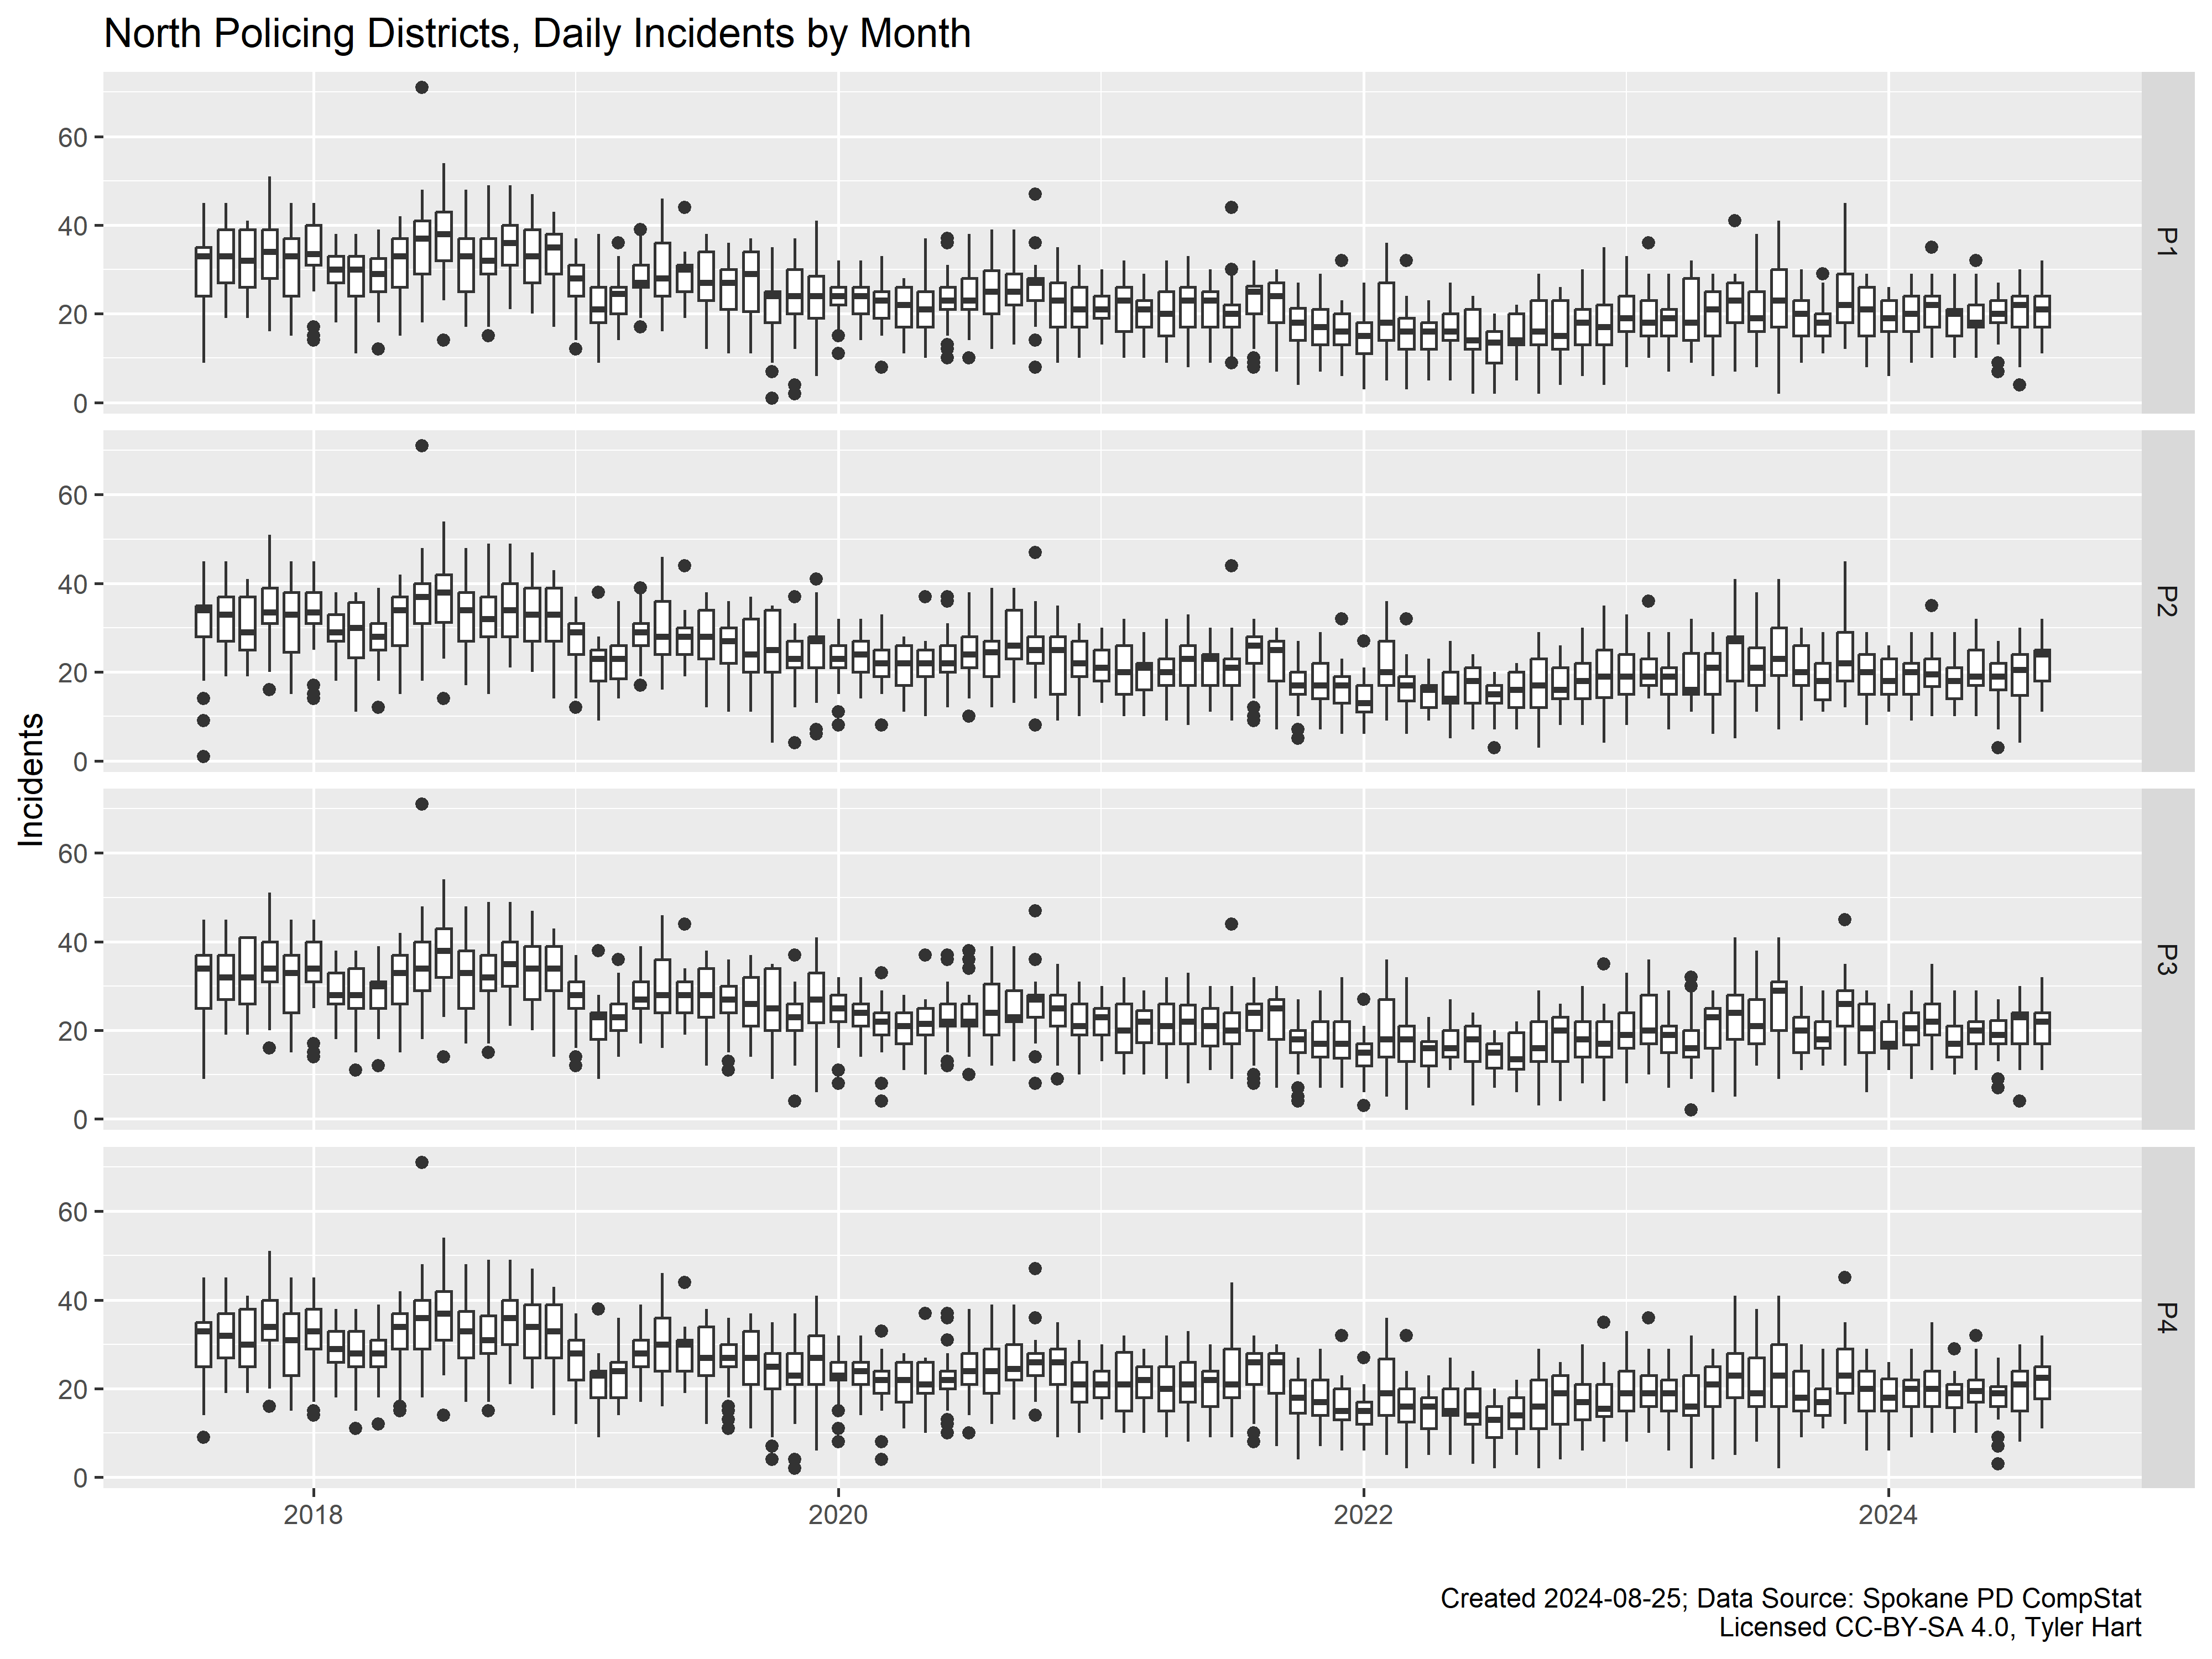
\includegraphics[width=\textwidth]{./figures/plot.boxplot_p1_p4_avg_daily_by_month-1} \end{center}

\begin{center}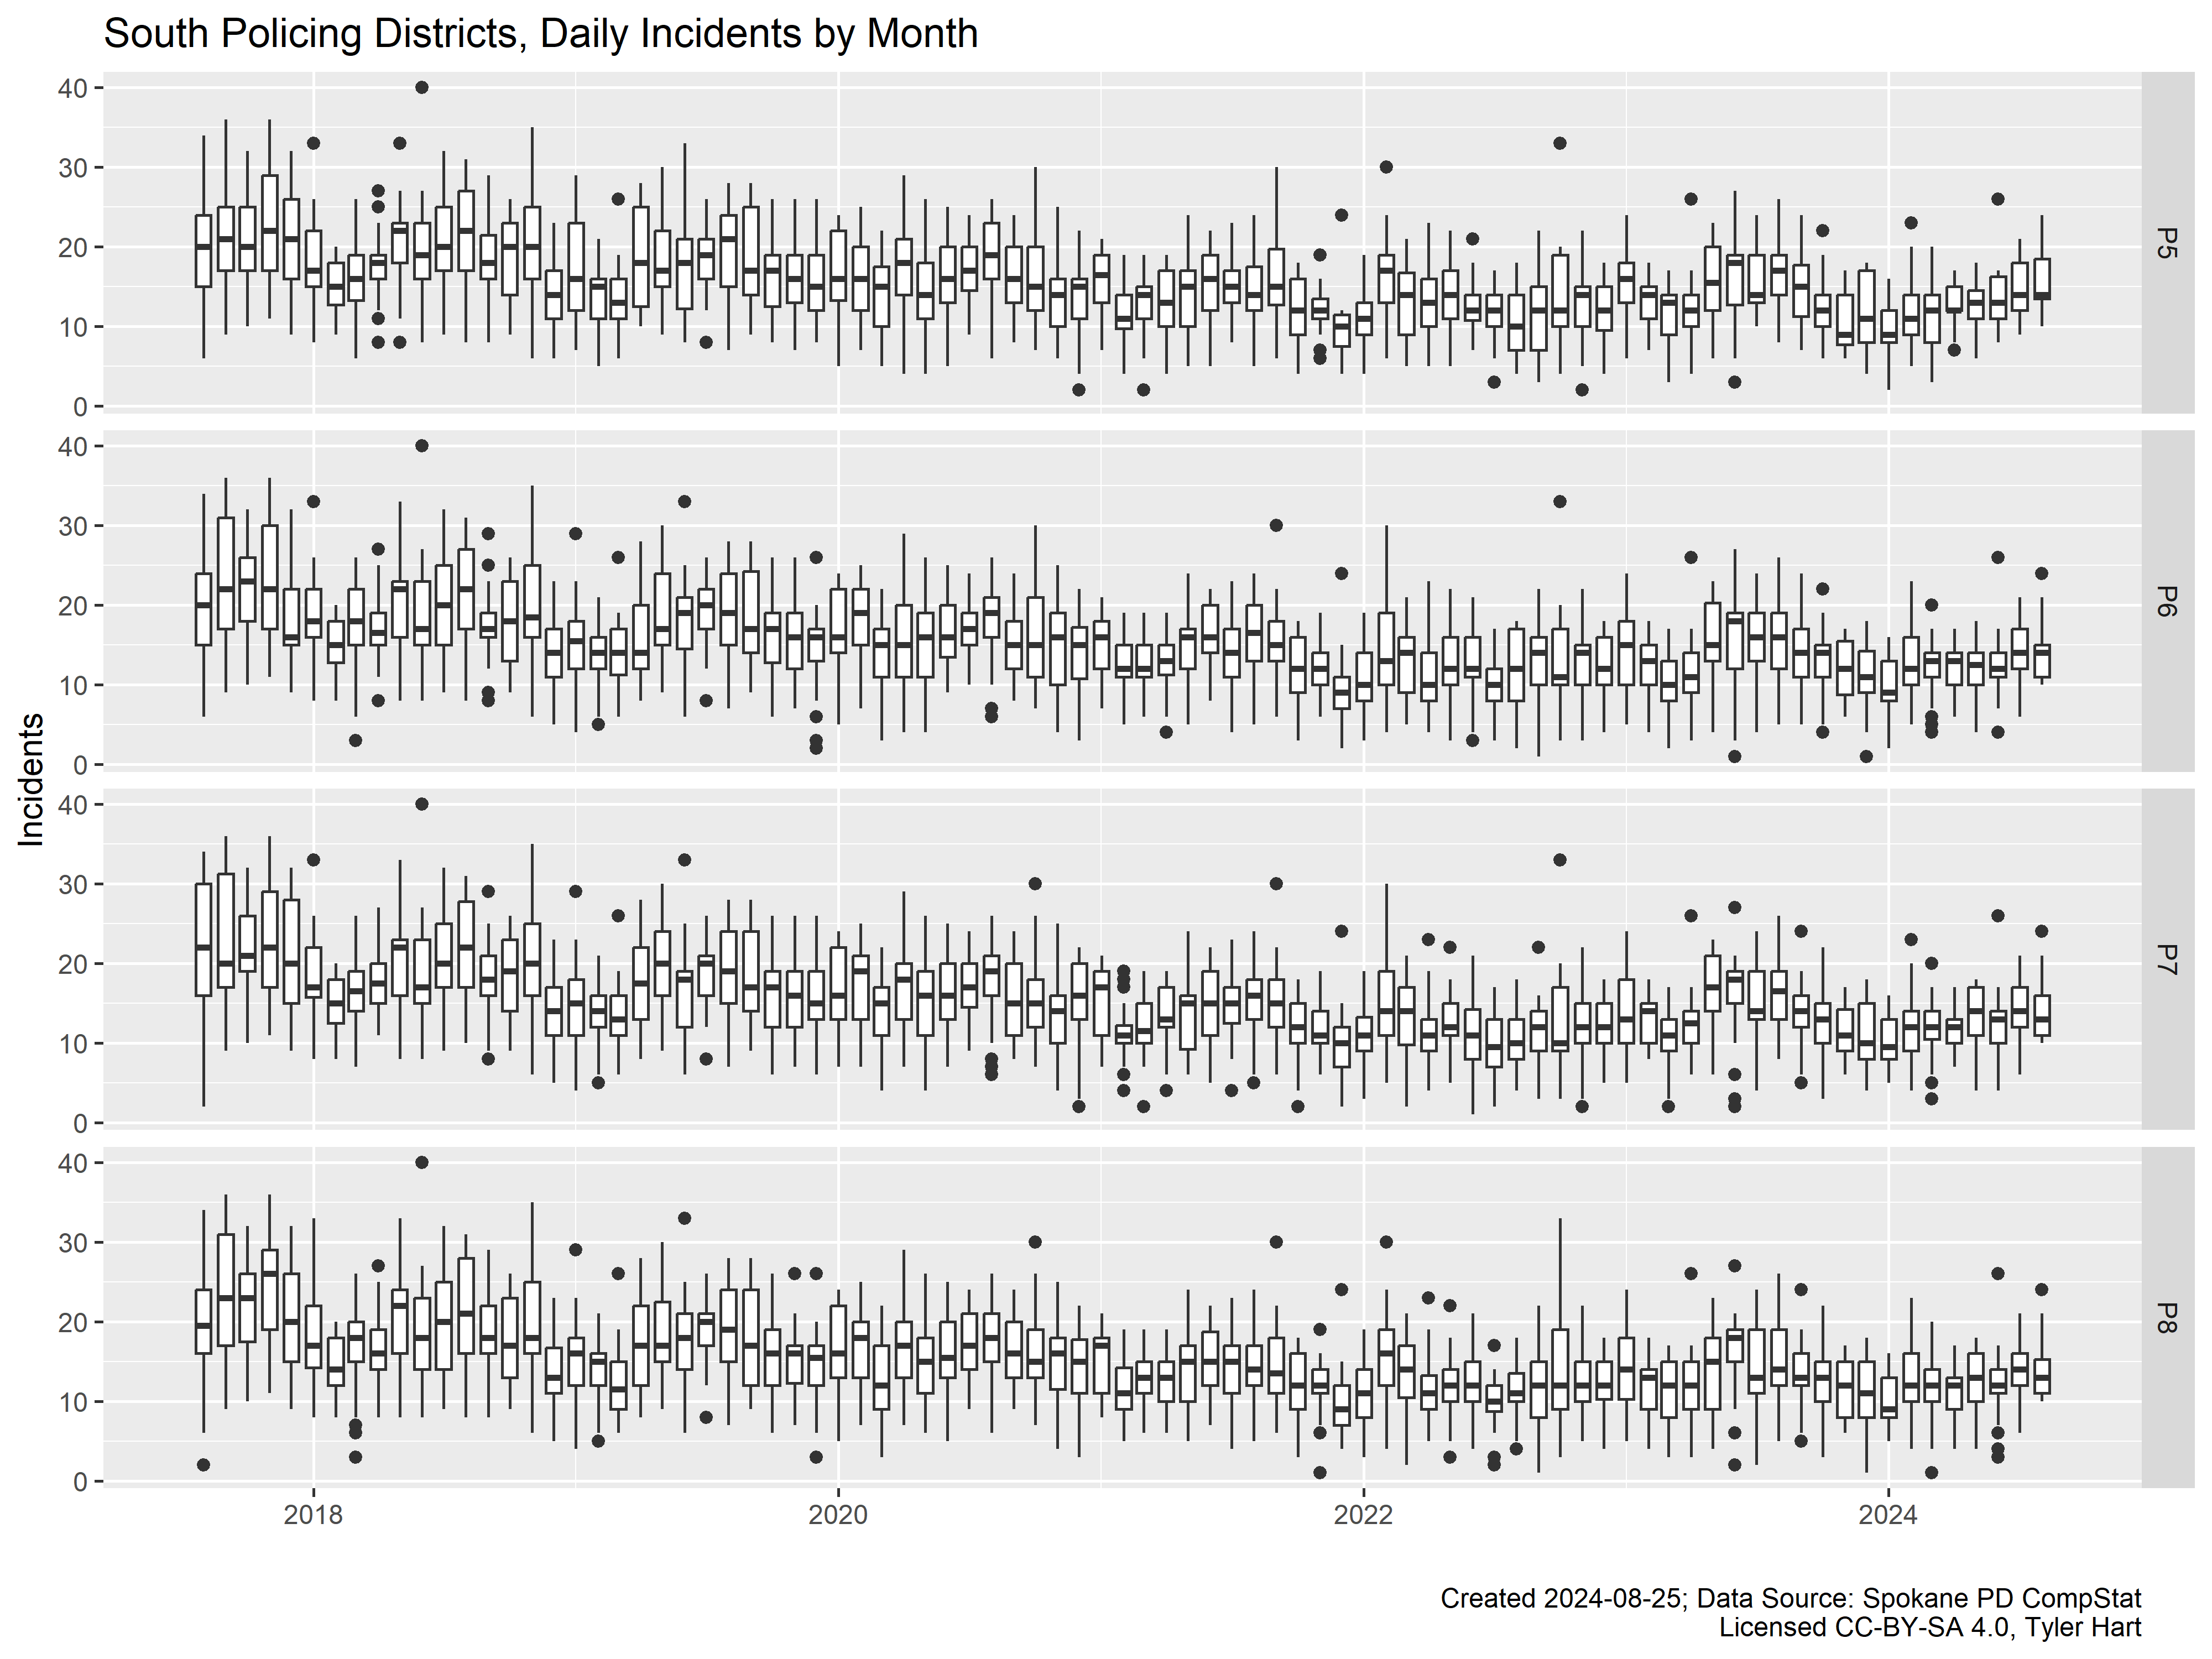
\includegraphics[width=\textwidth]{./figures/plot.boxplot_p5_p8_avg_daily_by_month-1} \end{center}

\begin{center}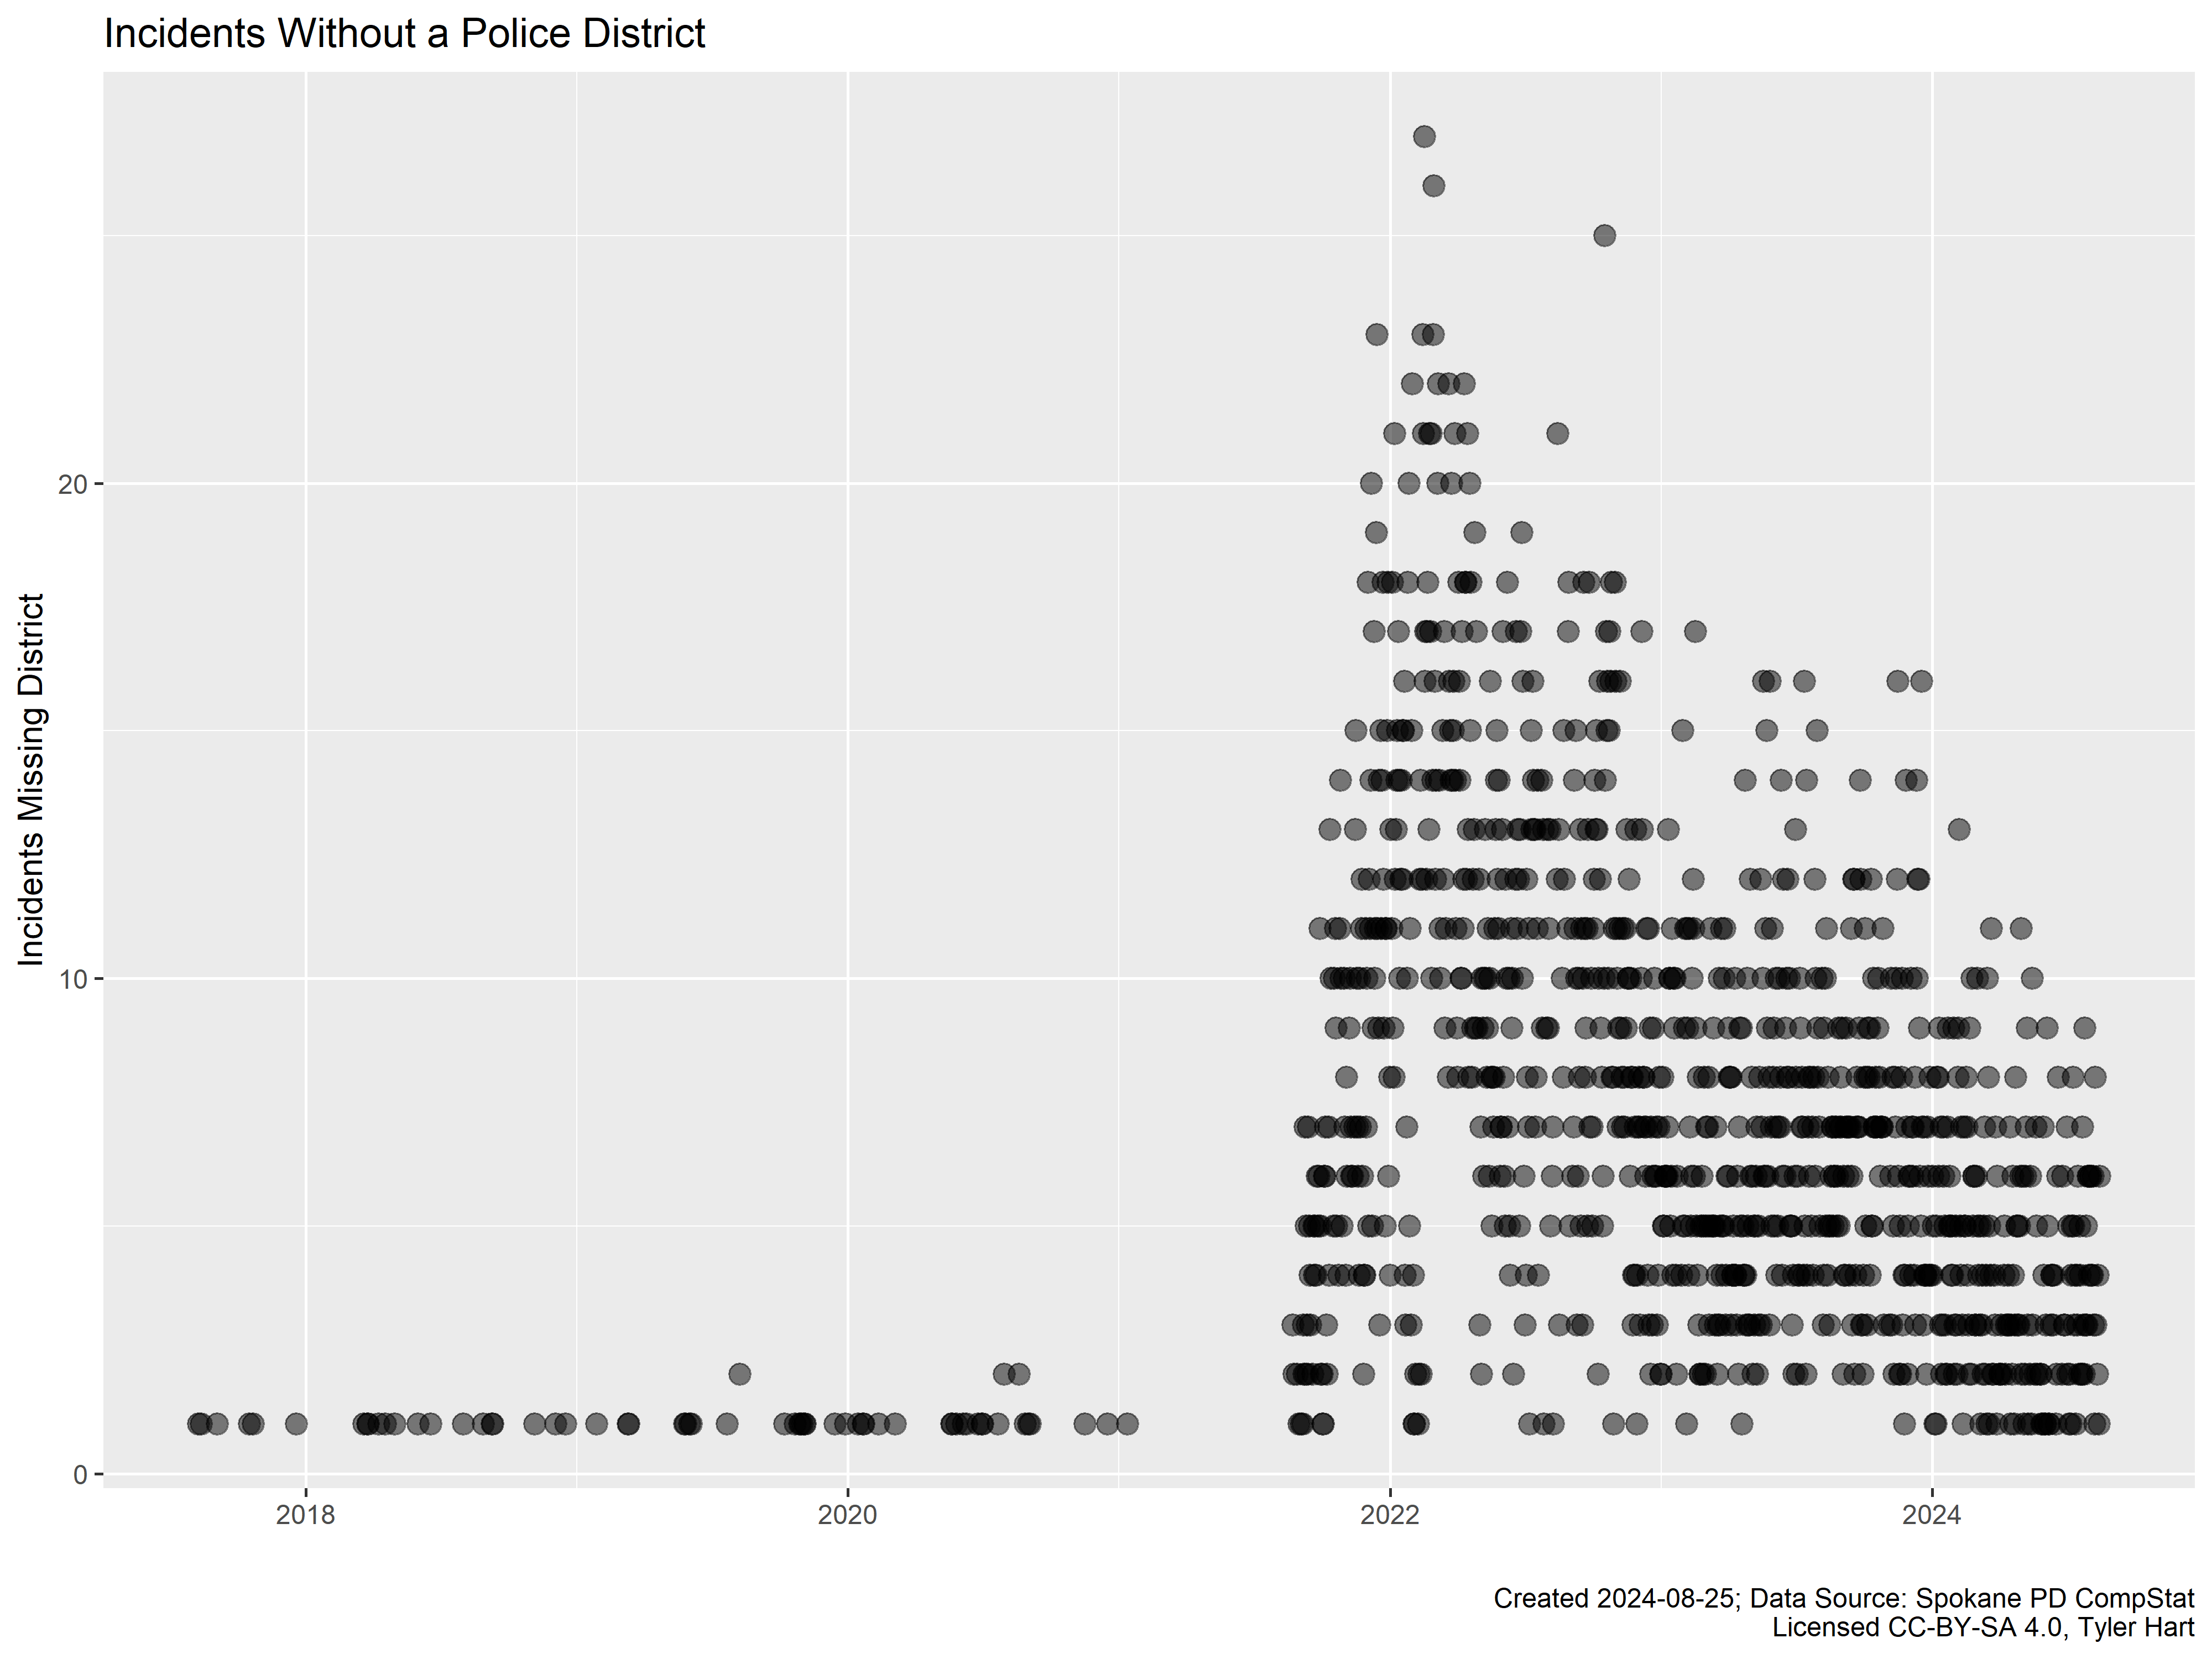
\includegraphics[width=\textwidth]{./figures/plot.district_nas_over_time-1} \end{center}

\begin{center}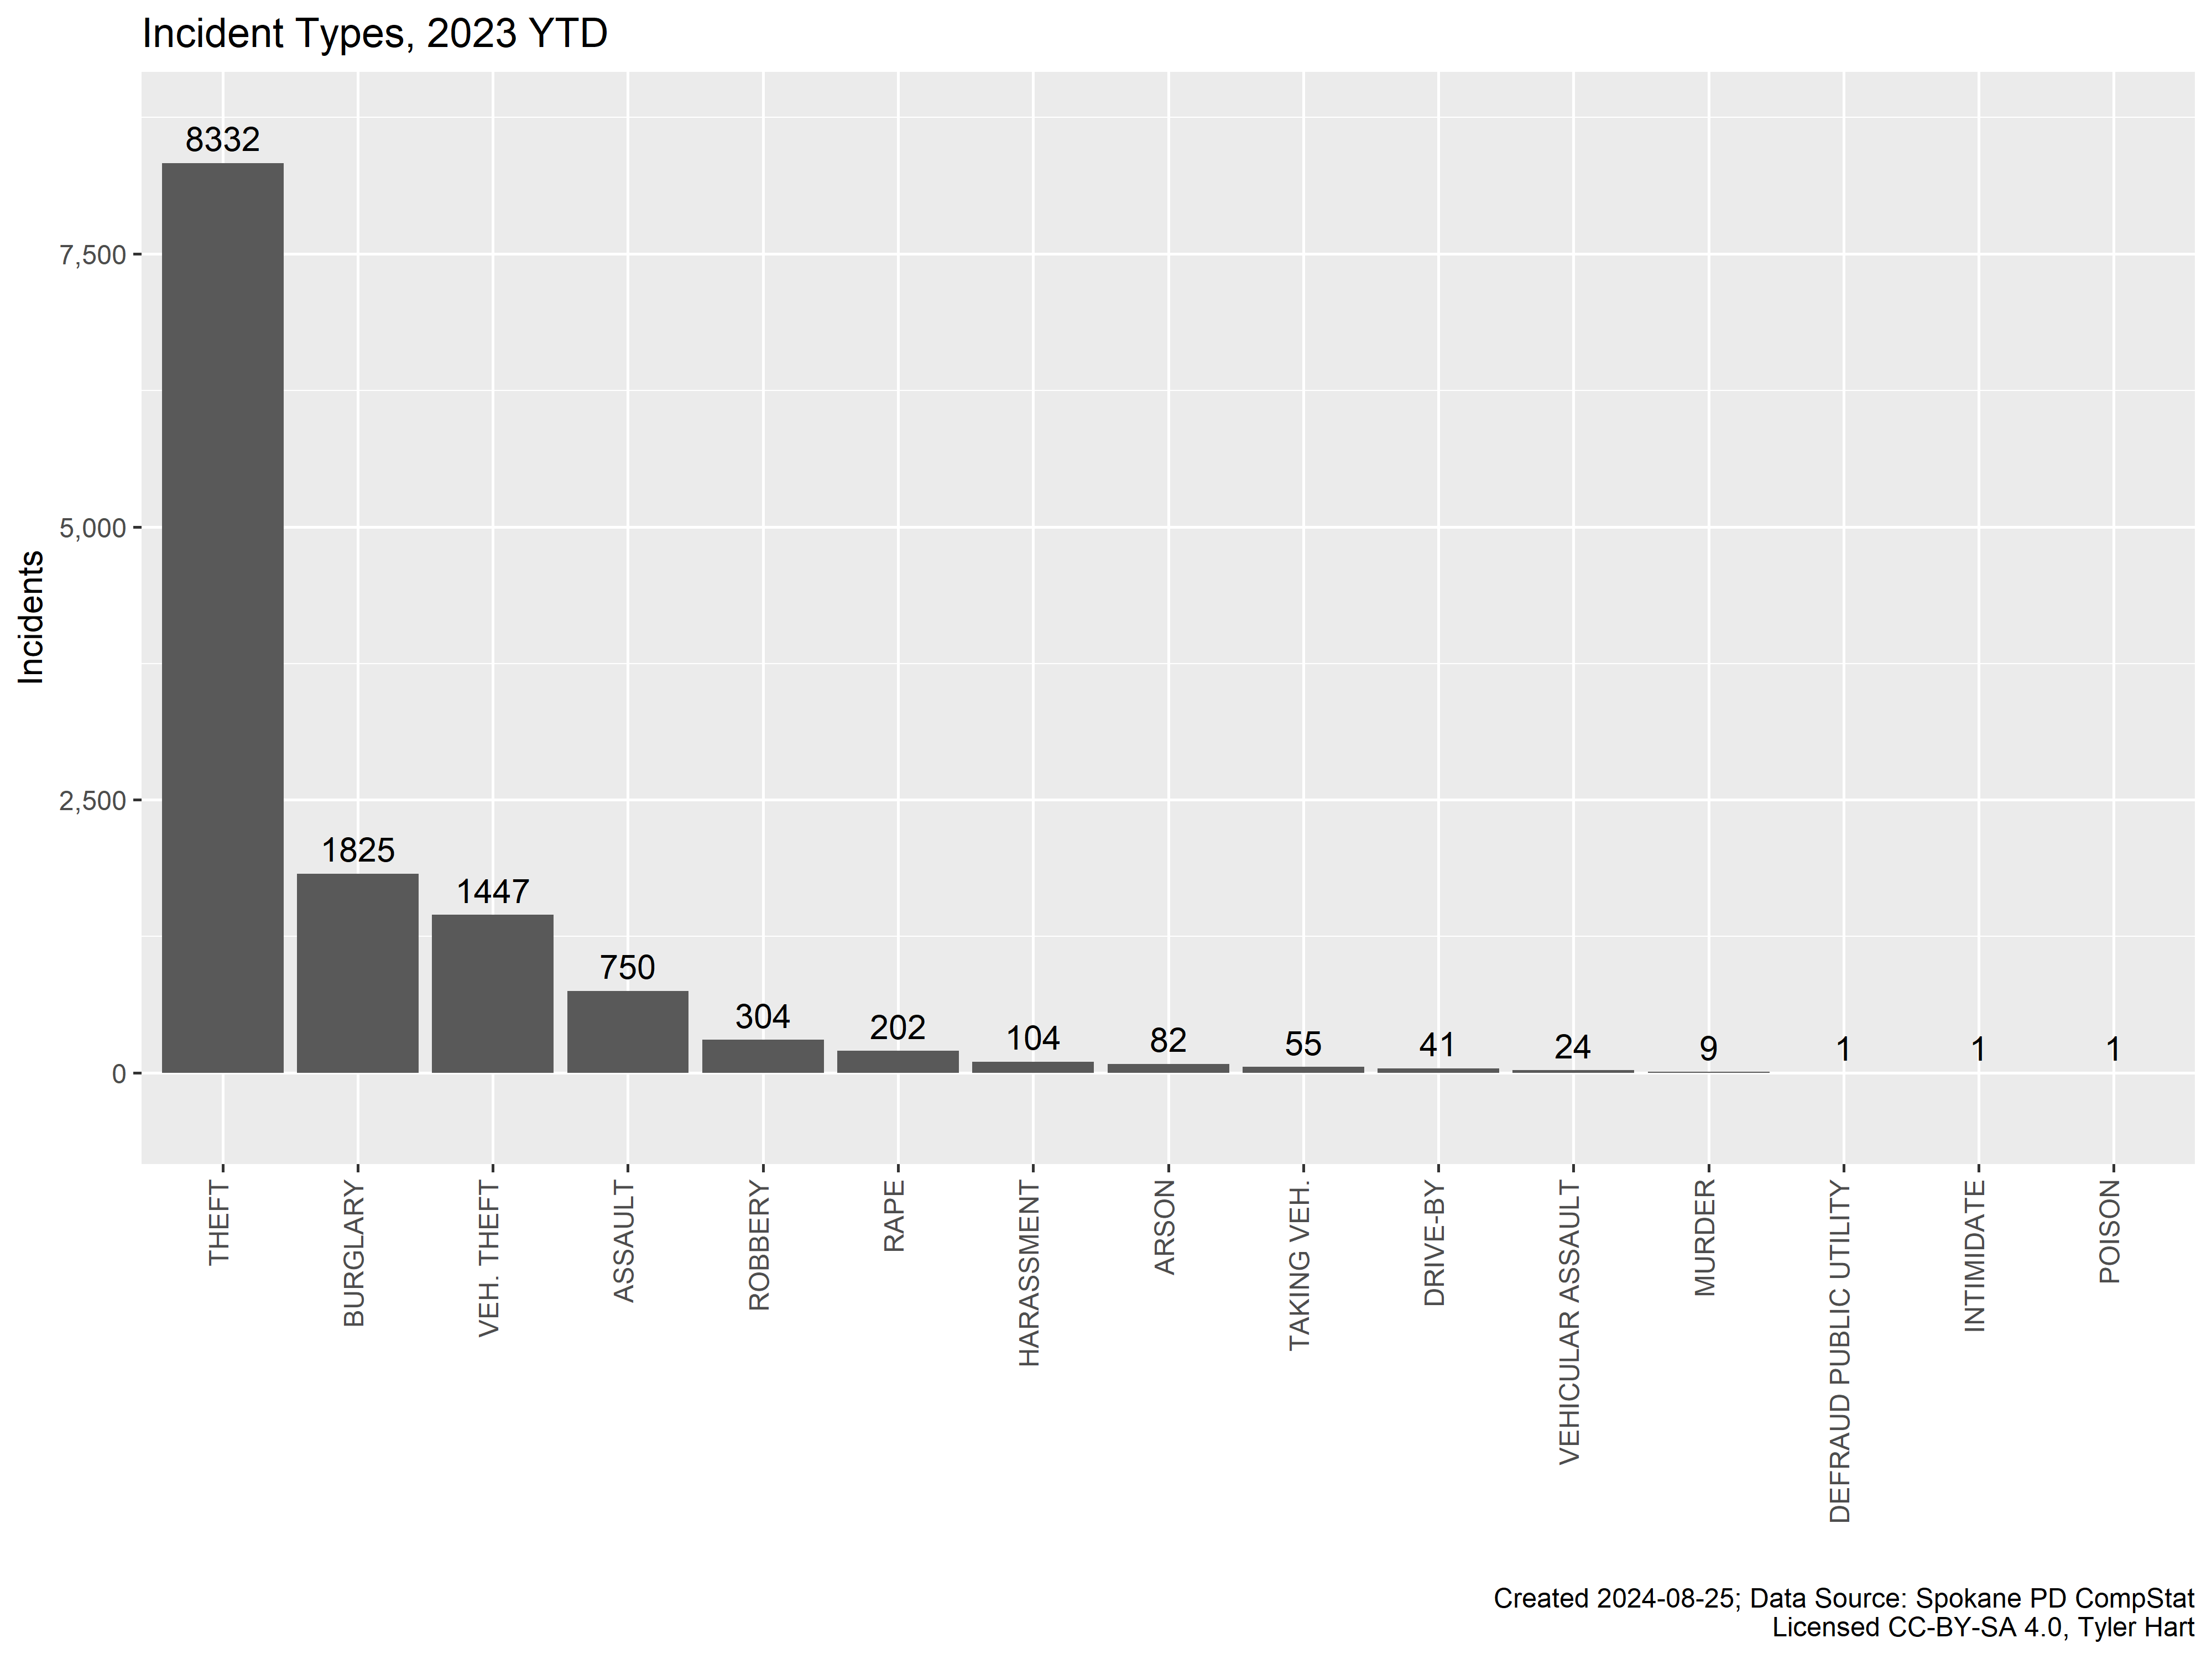
\includegraphics[width=\textwidth]{./figures/plot.ytd_offenses_by_type-1} \end{center}

\begin{center}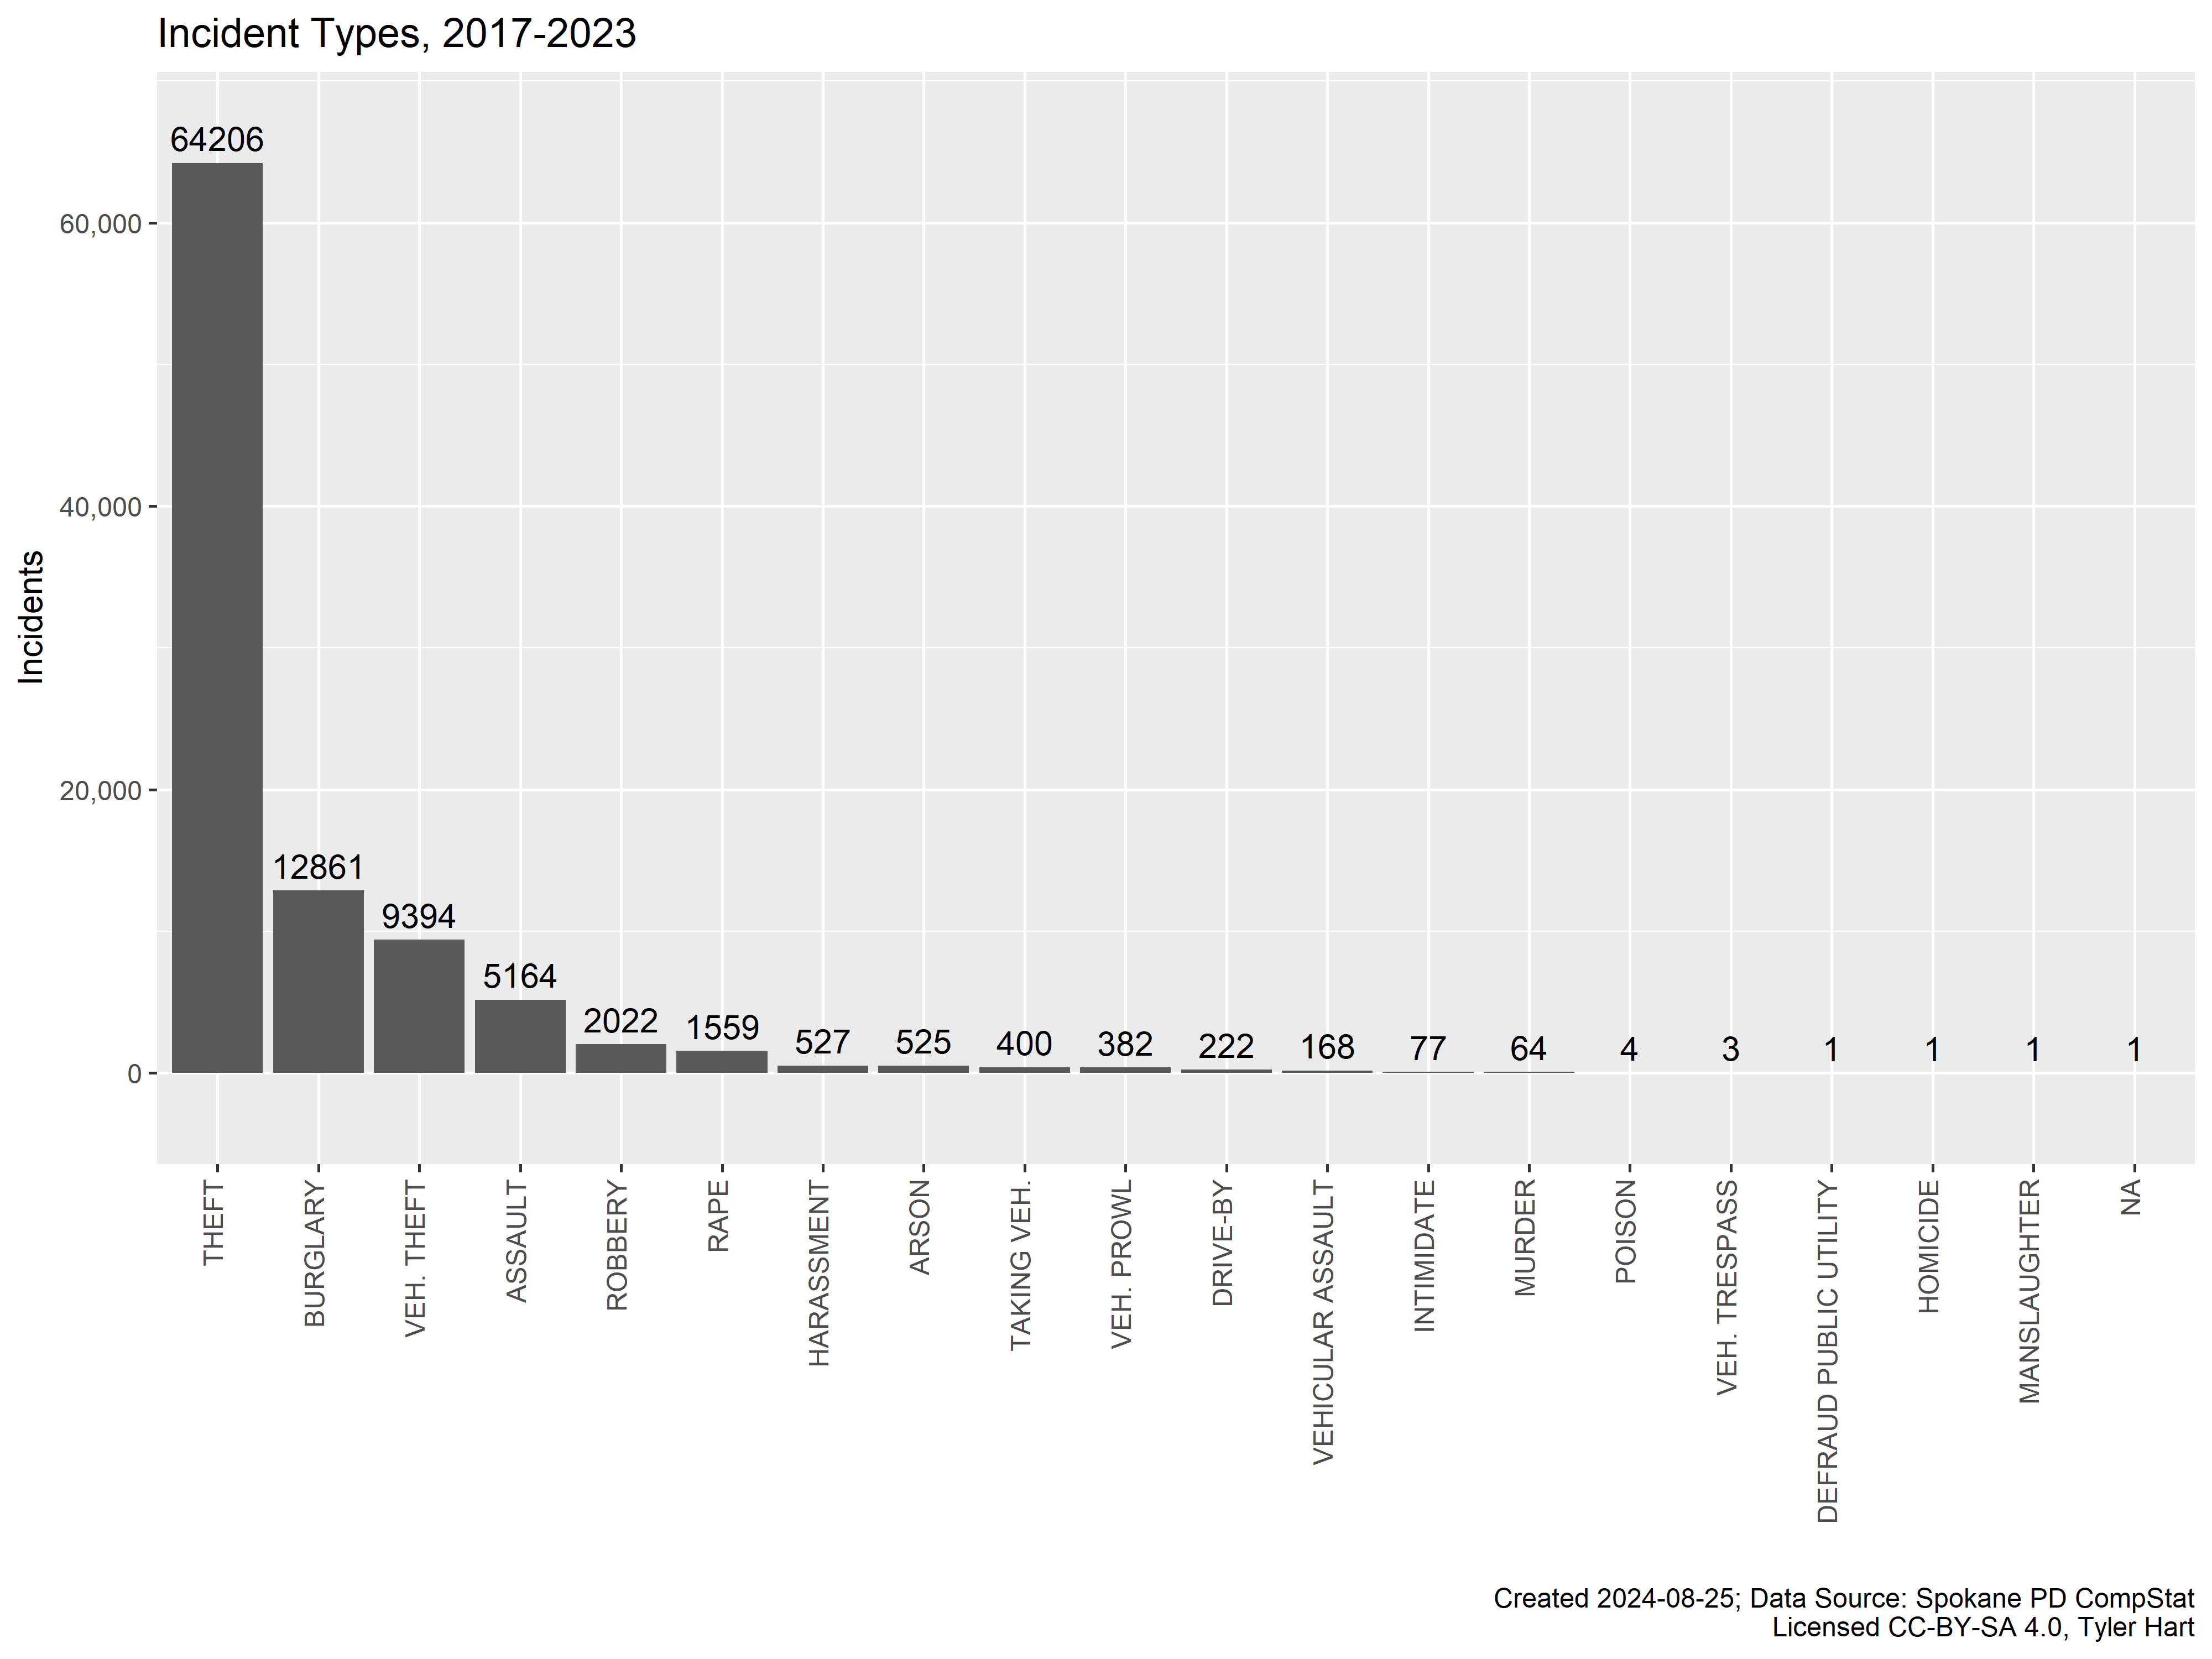
\includegraphics[width=\textwidth]{./figures/plot.total_offenses_by_type-1} \end{center}

\begin{center}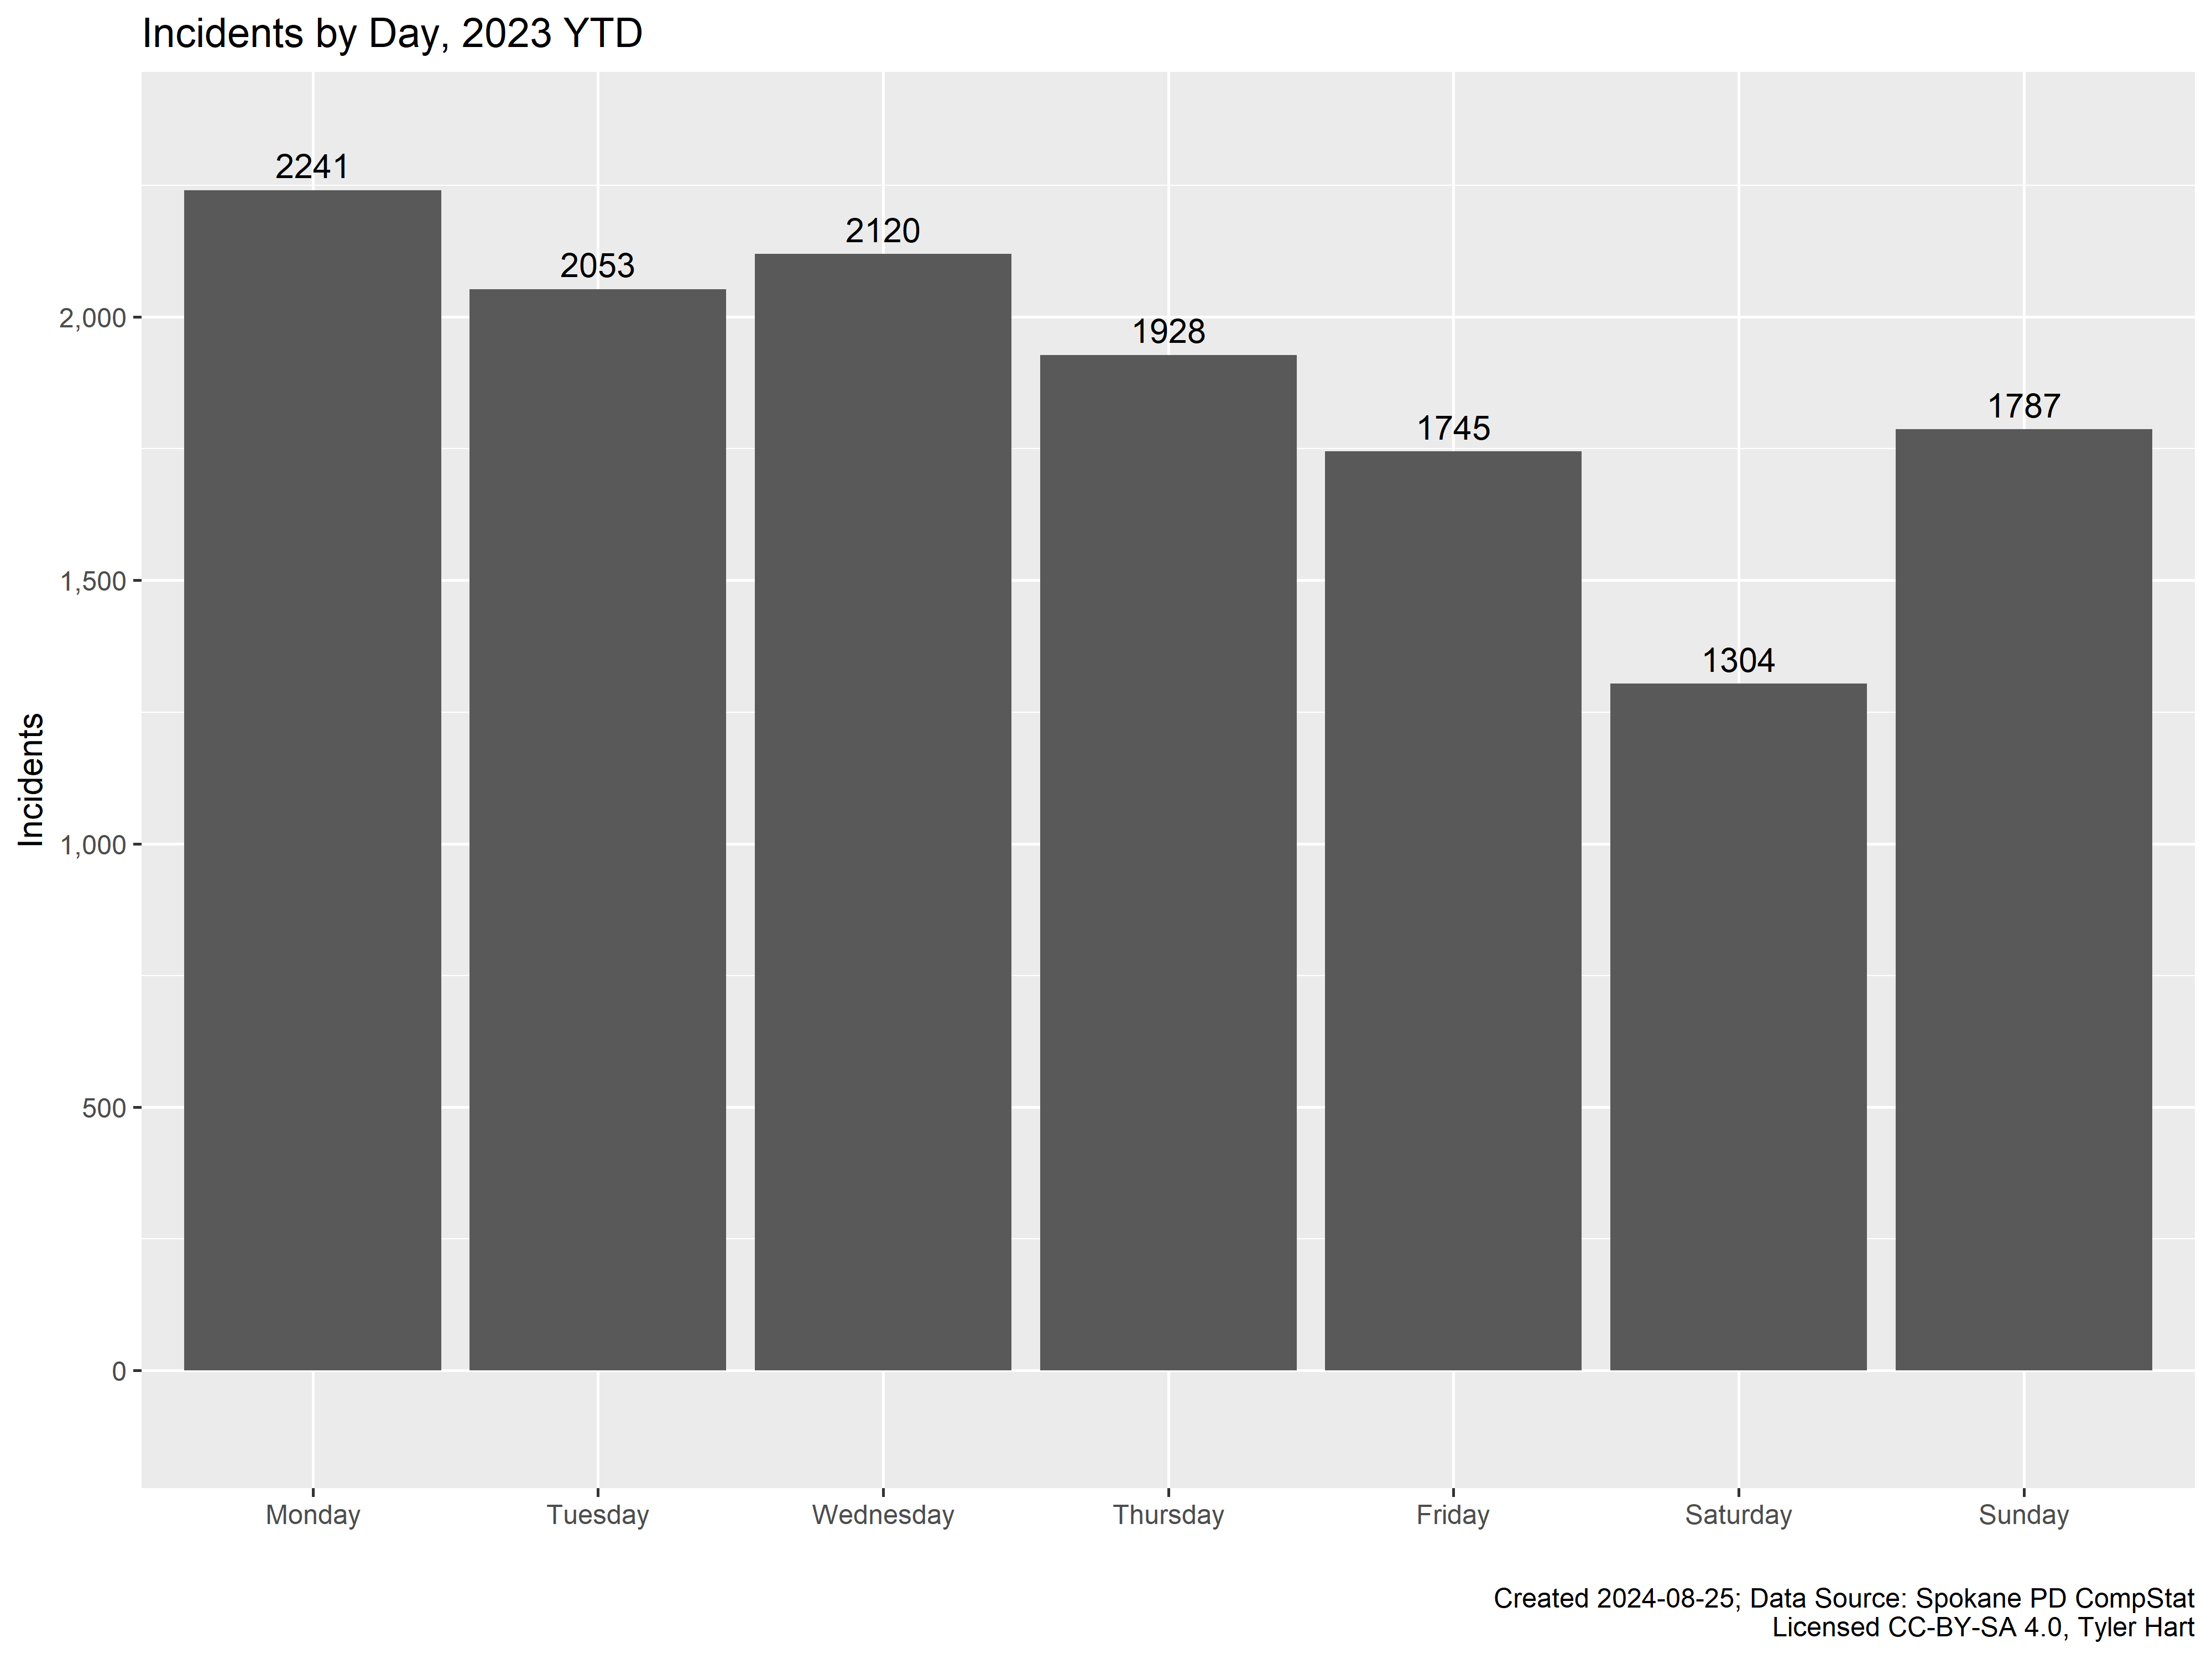
\includegraphics[width=\textwidth]{./figures/plot.ytd_offenses_by_weekday-1} \end{center}

\begin{center}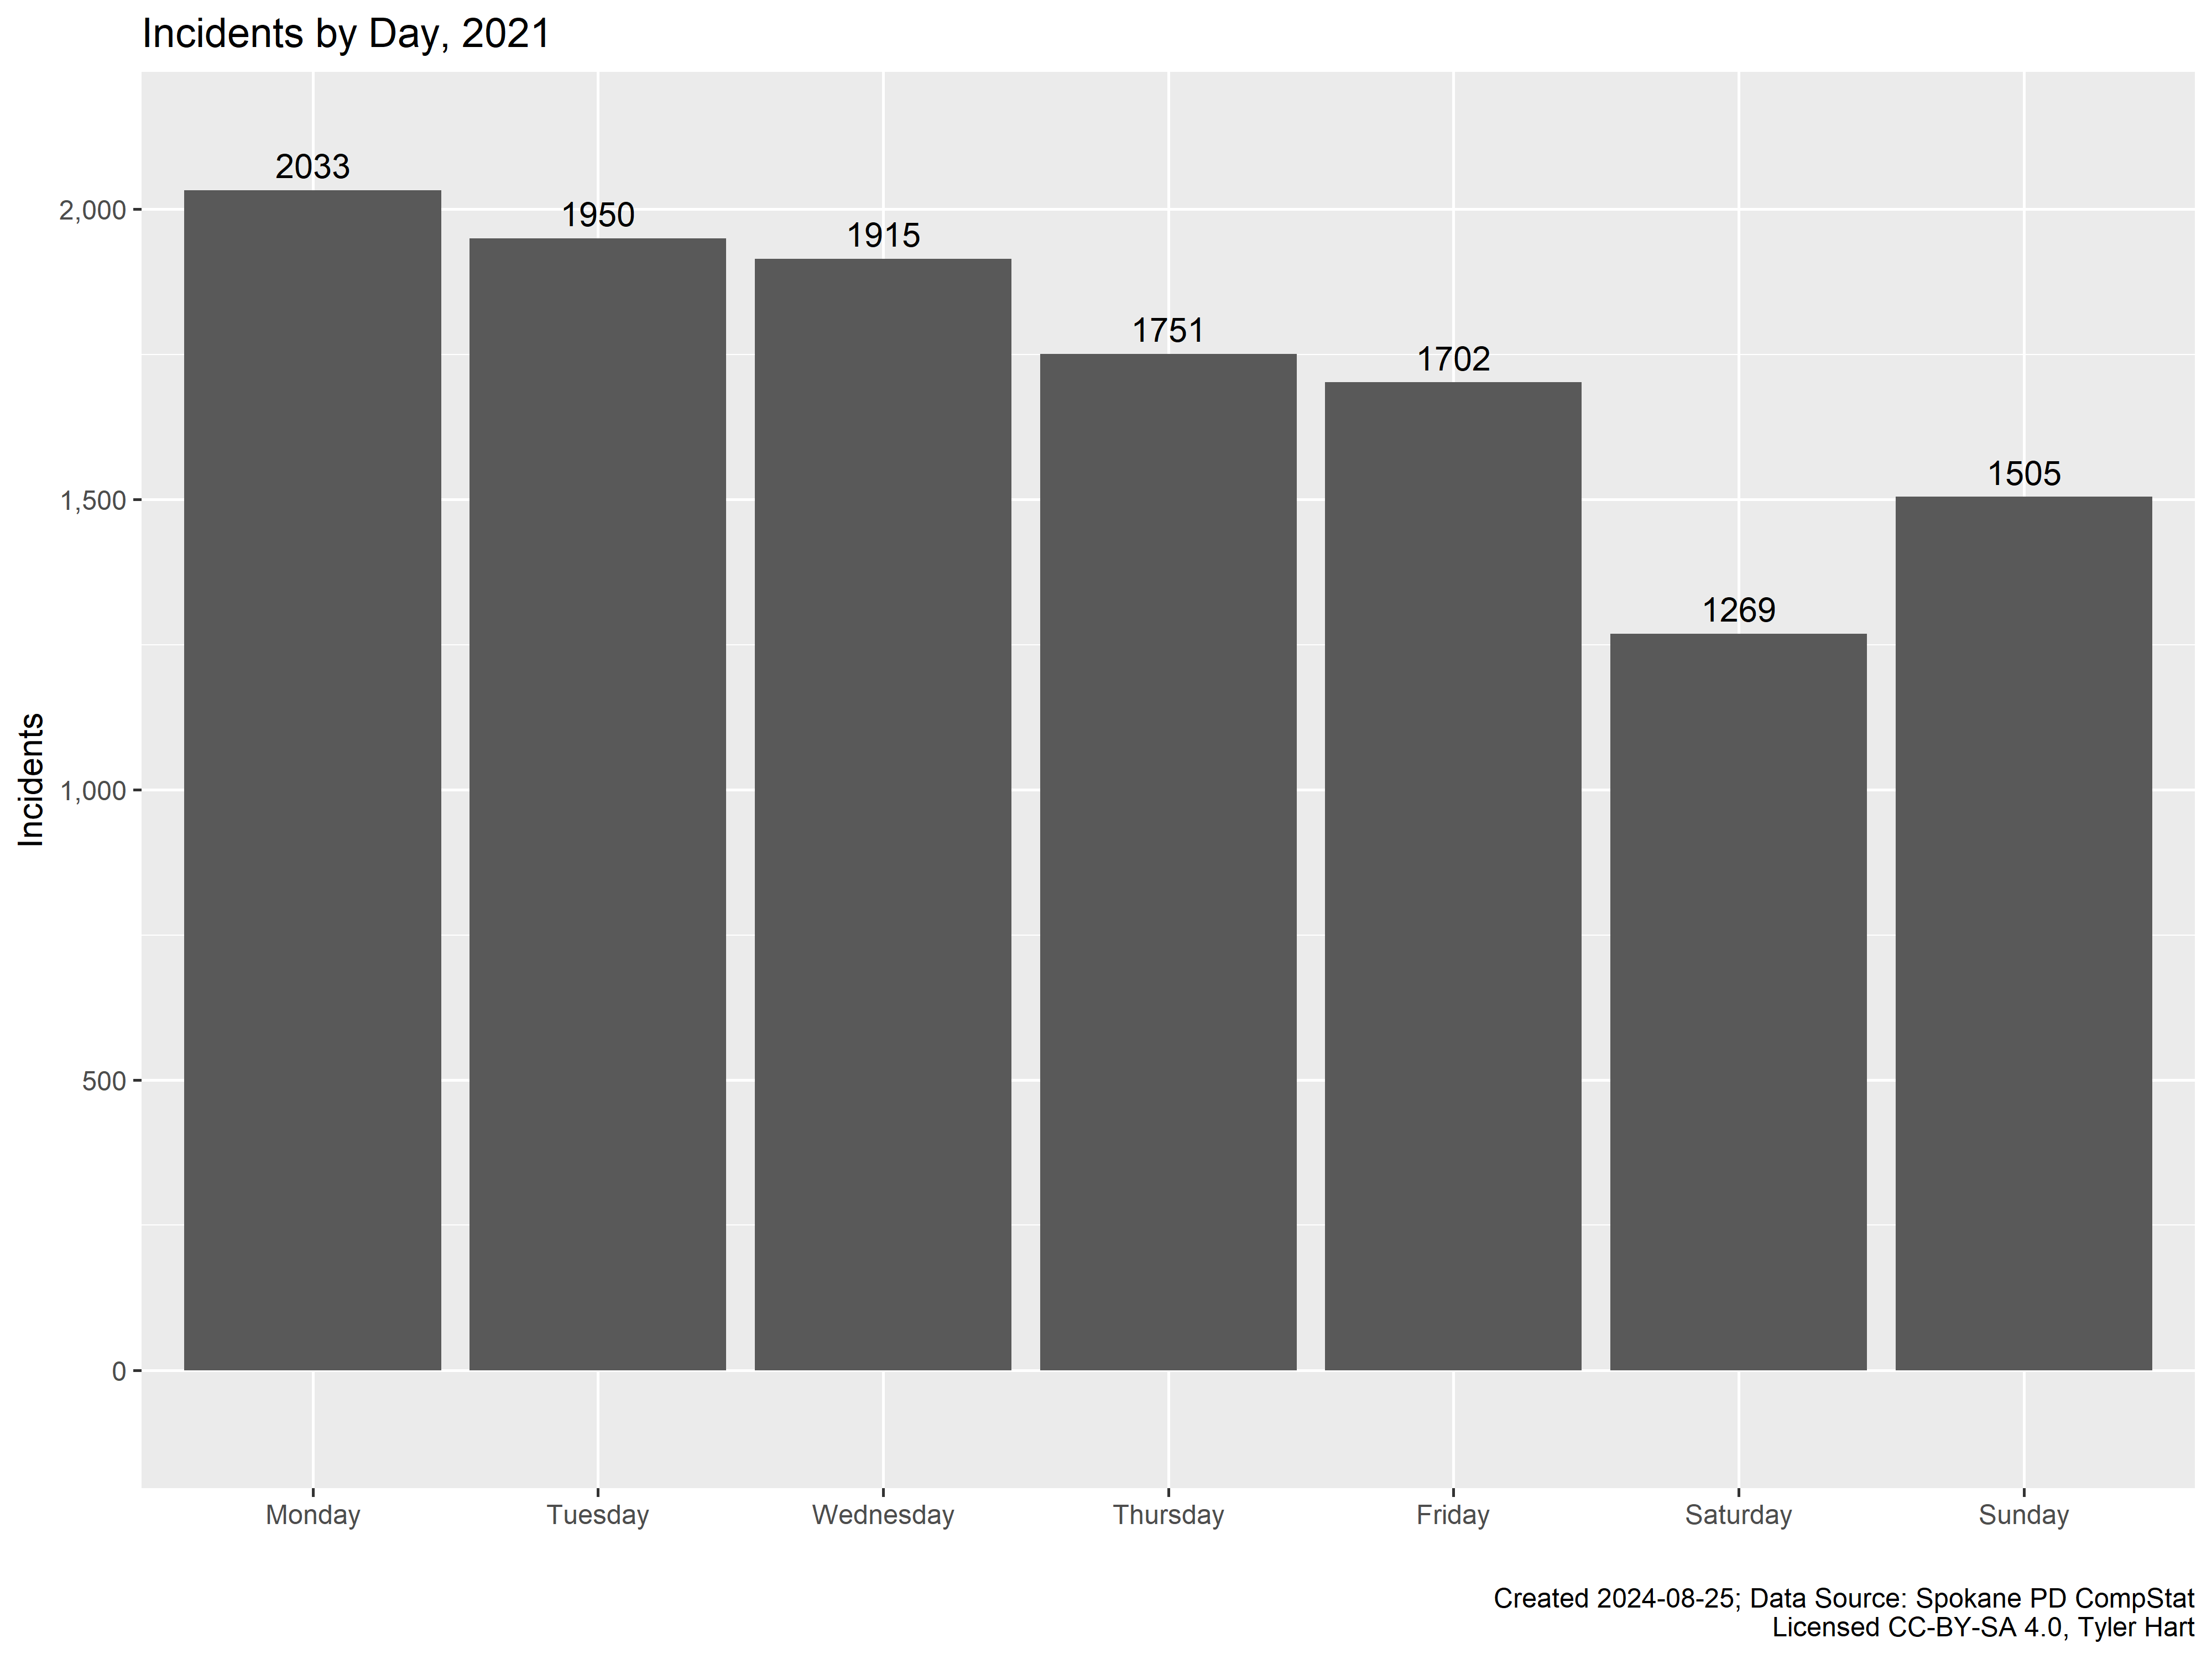
\includegraphics[width=\textwidth]{./figures/plot.2021_offenses_by_weekday-1} \end{center}

\begin{center}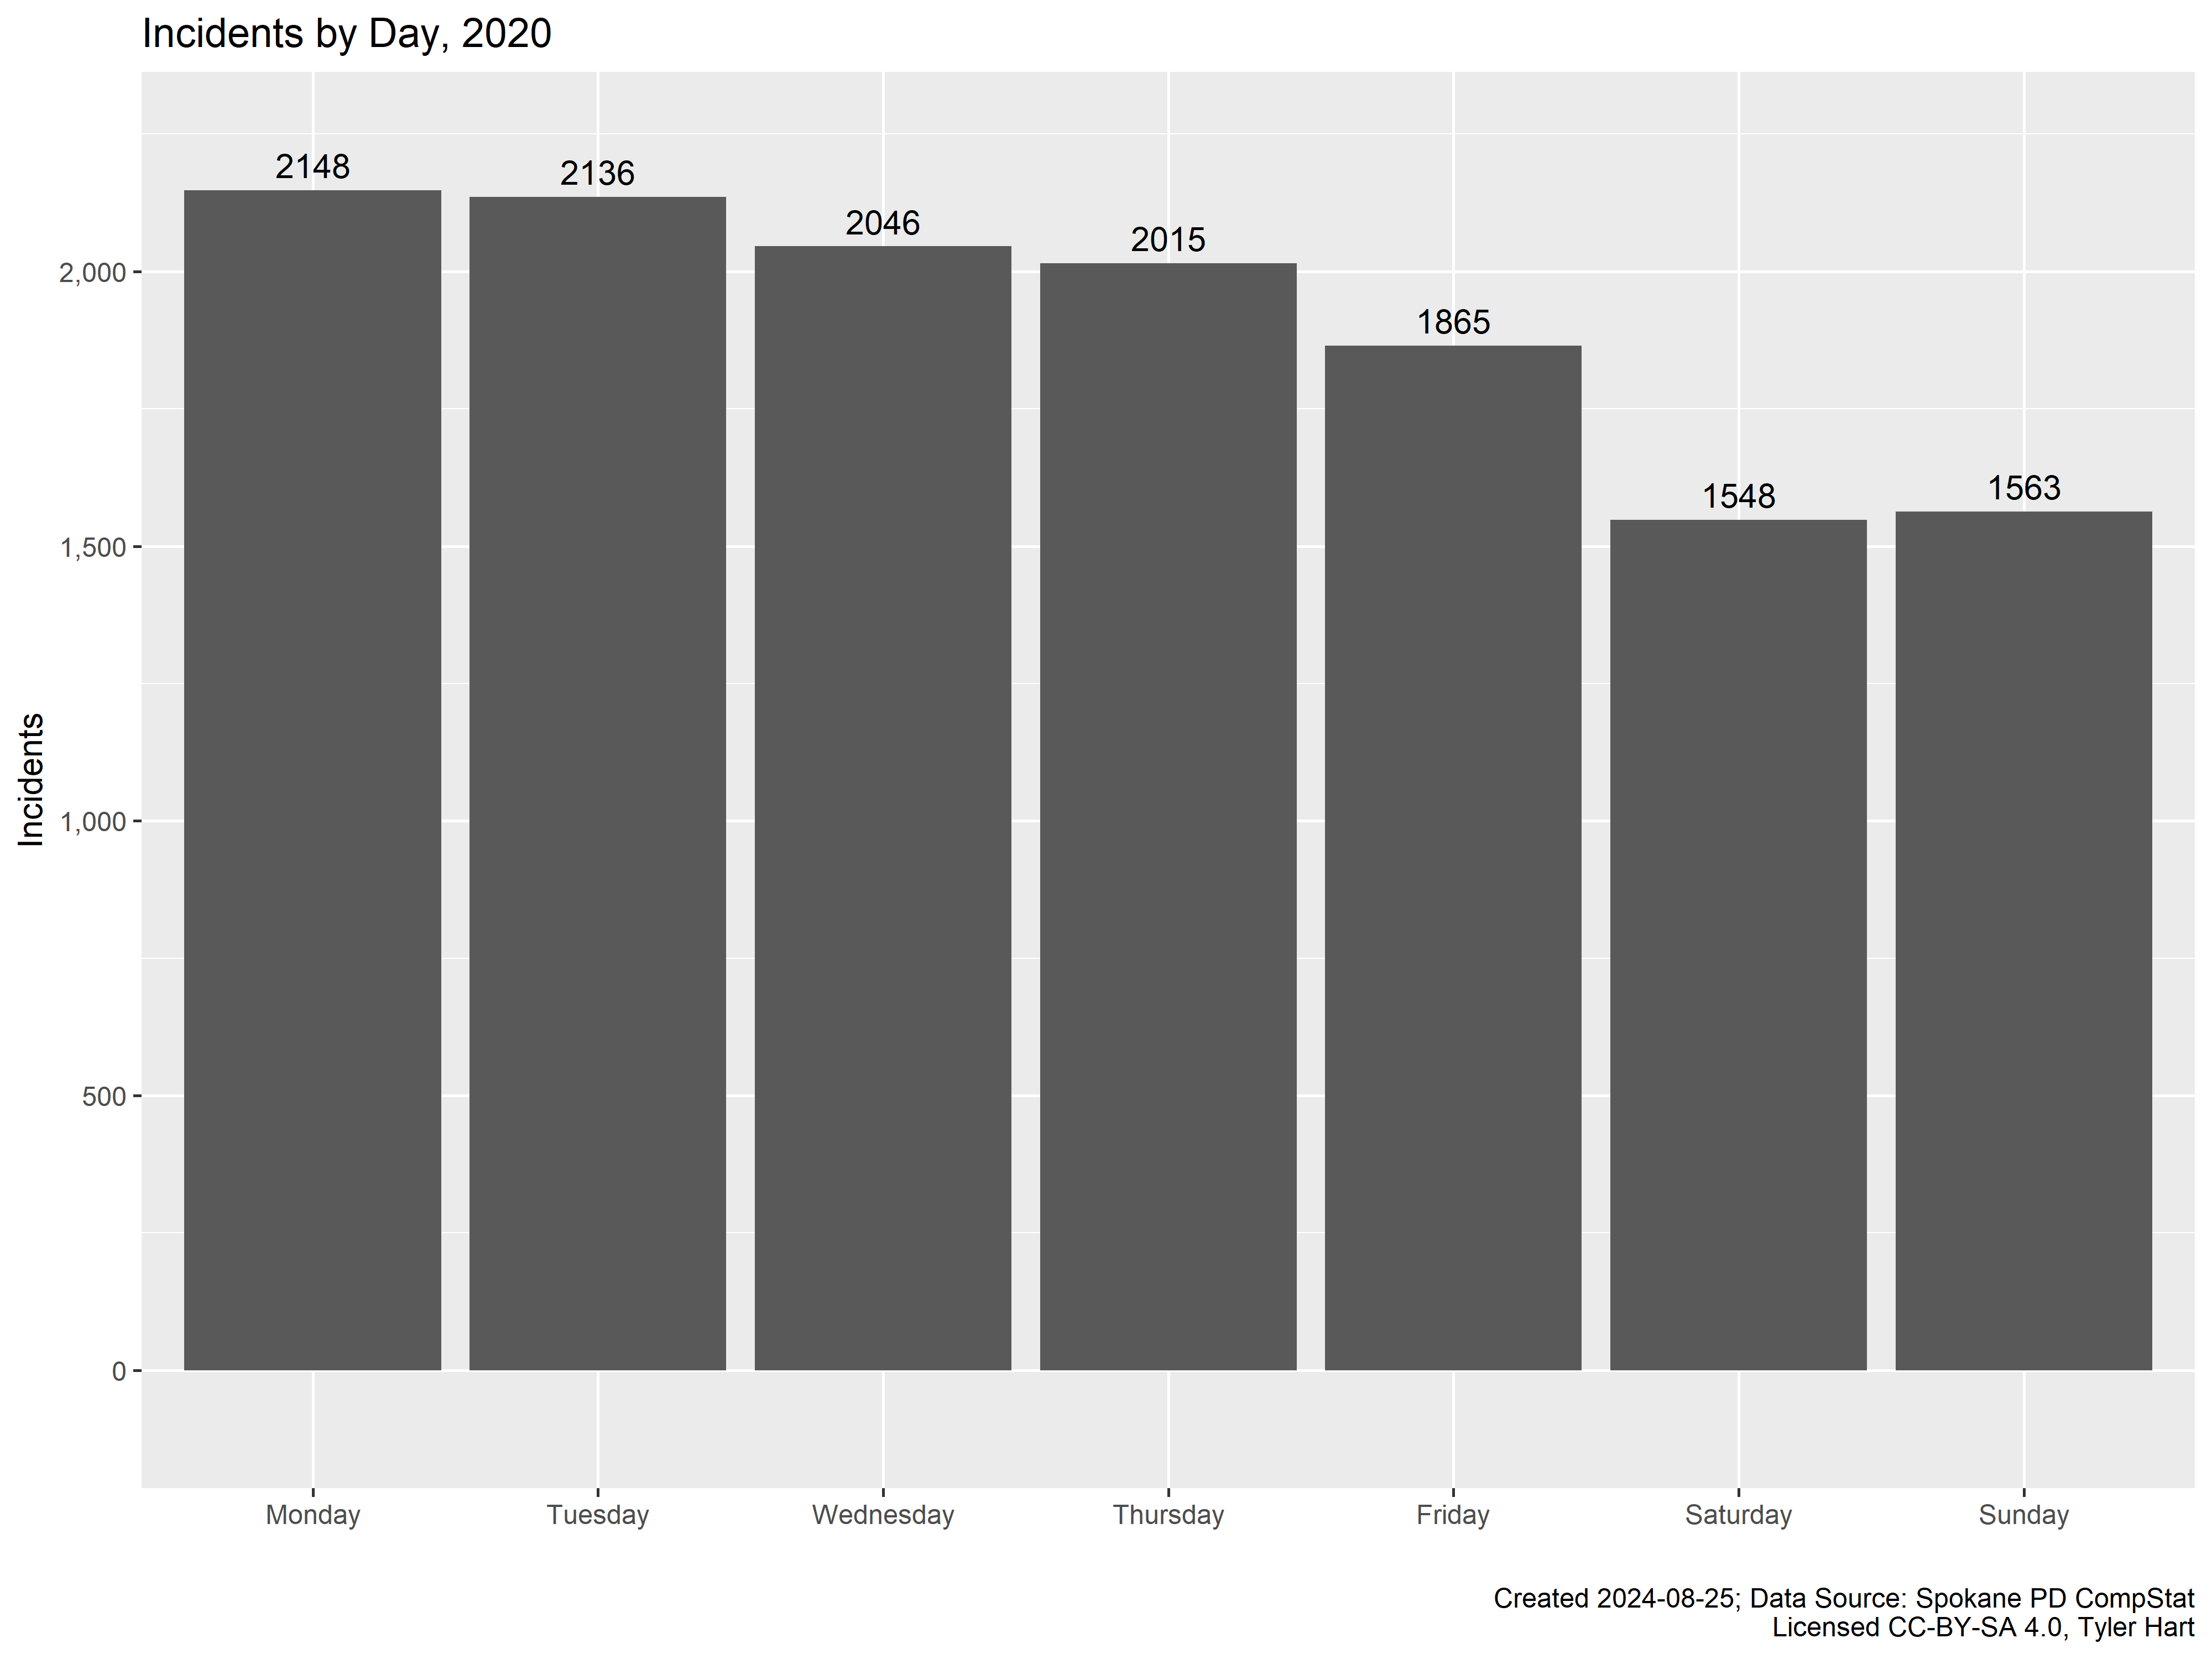
\includegraphics[width=\textwidth]{./figures/plot.2020_offenses_by_weekday-1} \end{center}

\begin{center}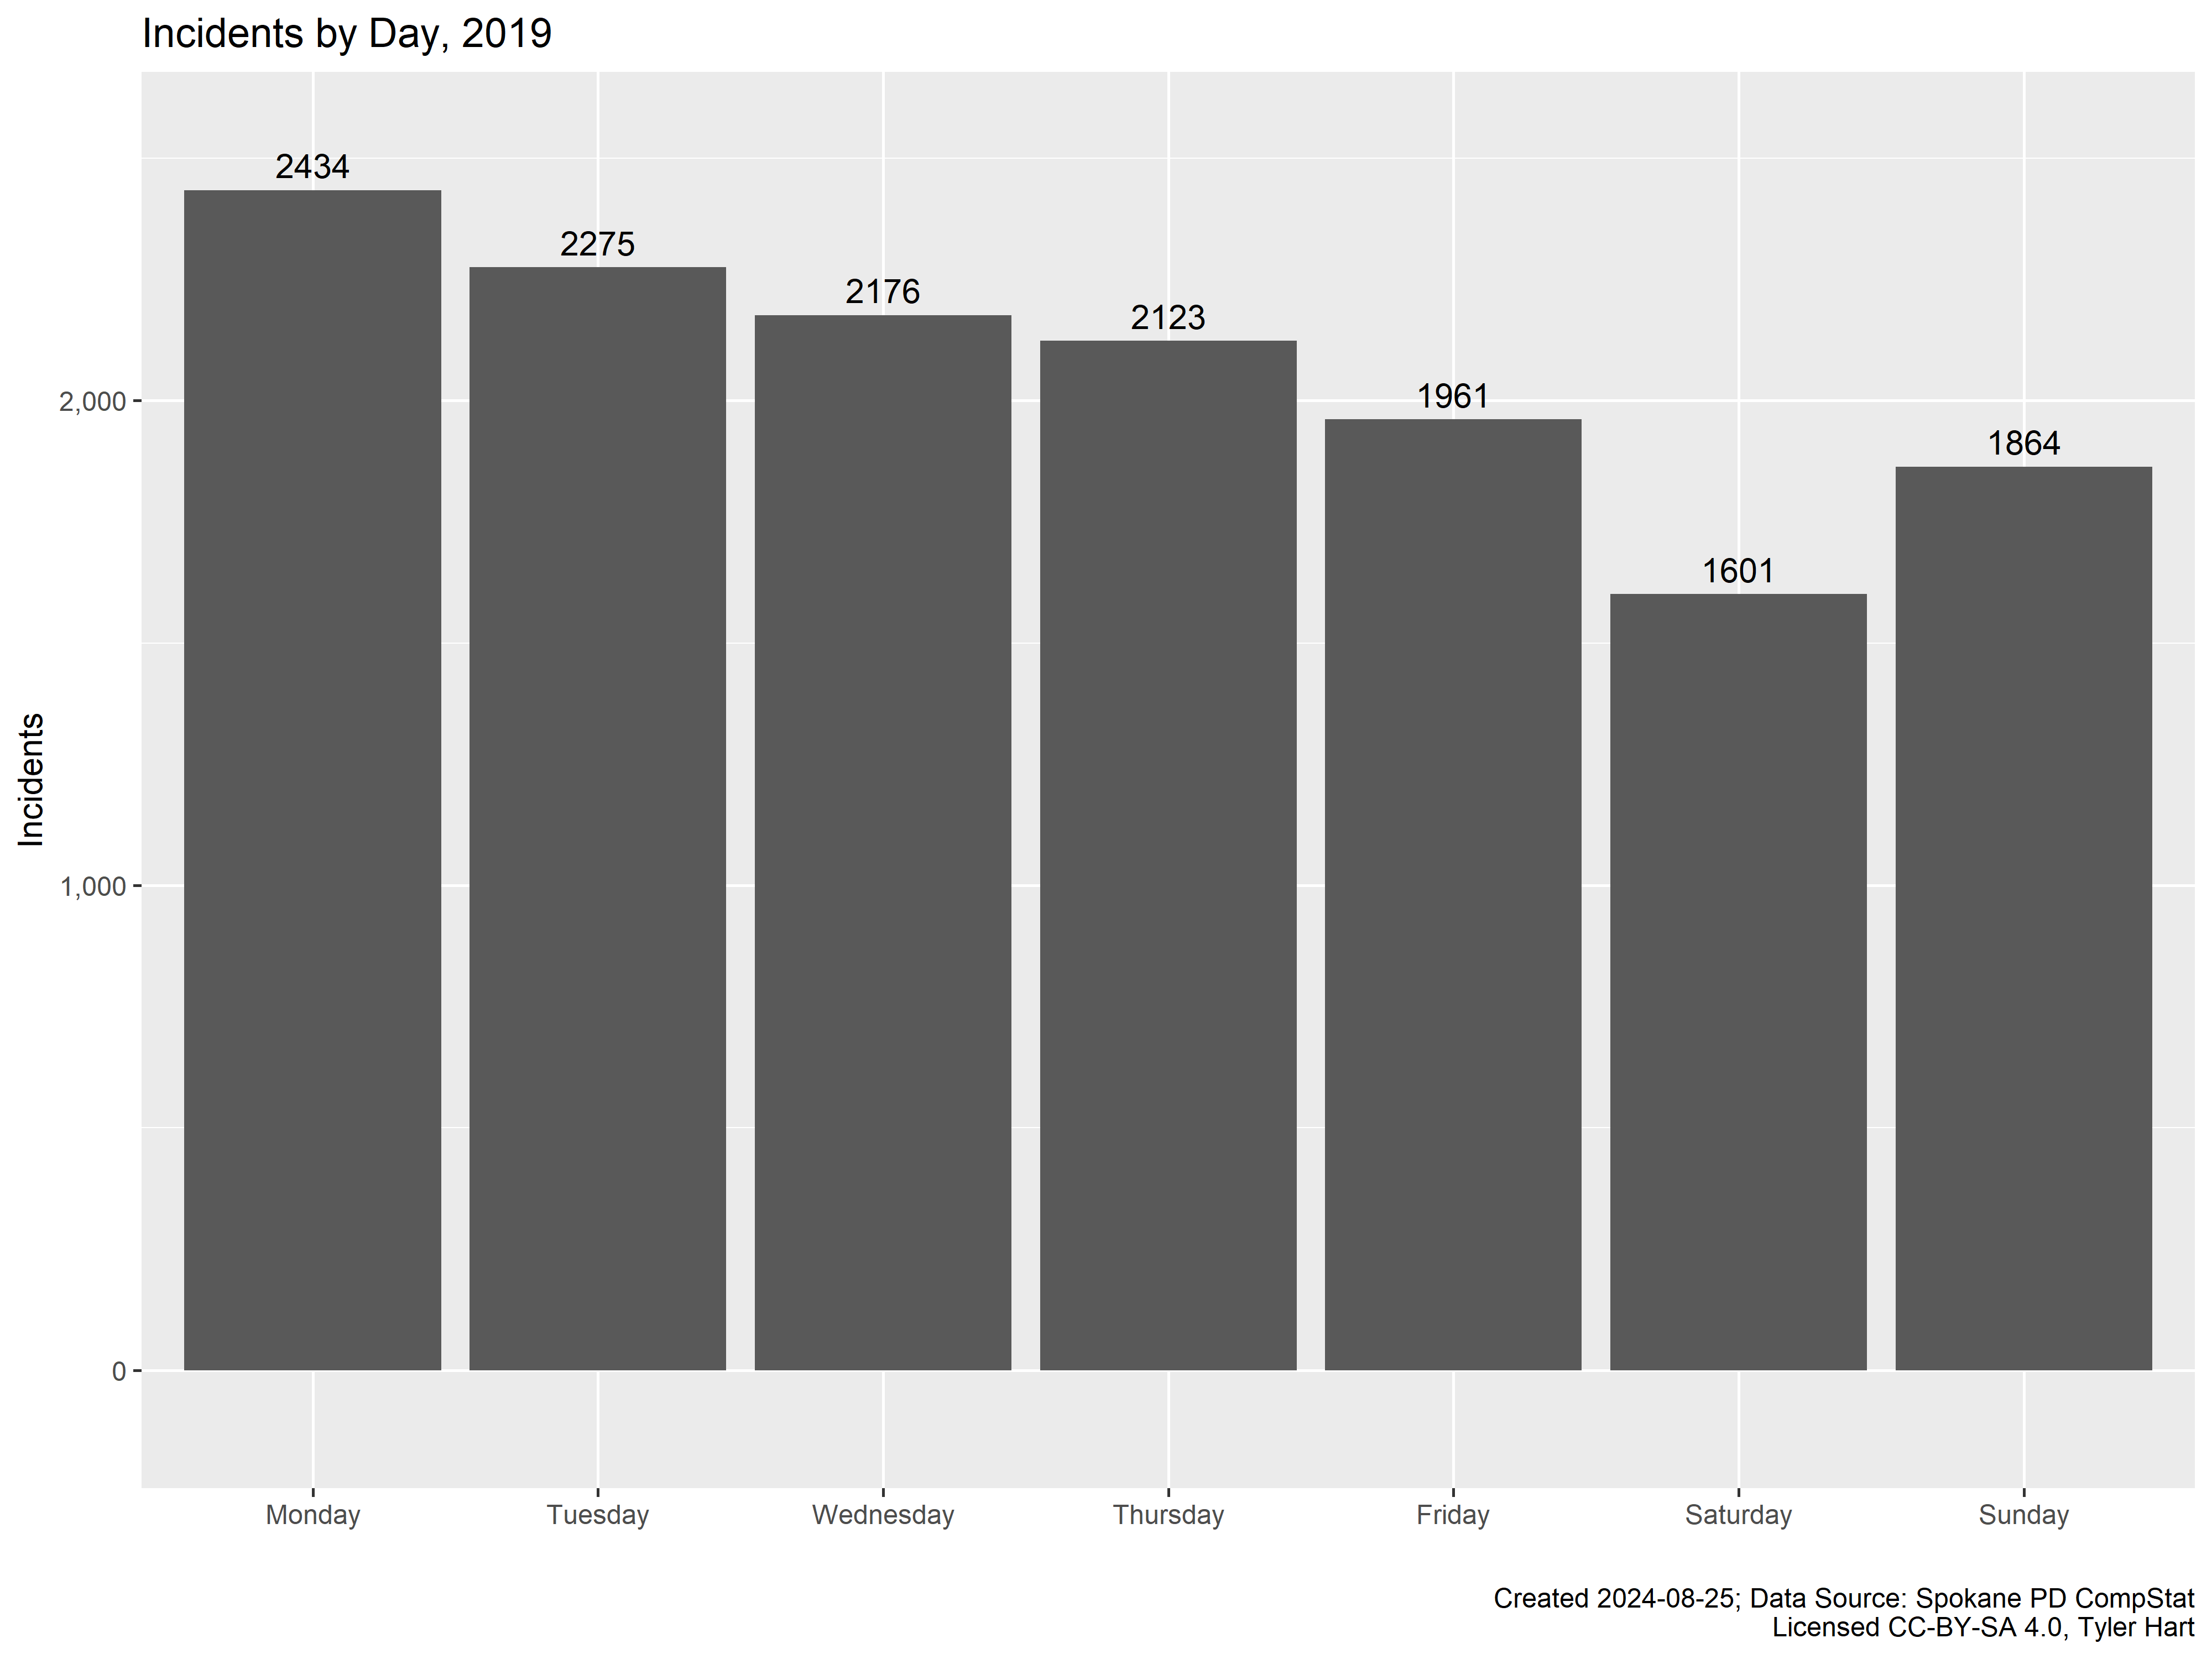
\includegraphics[width=\textwidth]{./figures/plot.2019_offenses_by_weekday-1} \end{center}

\begin{center}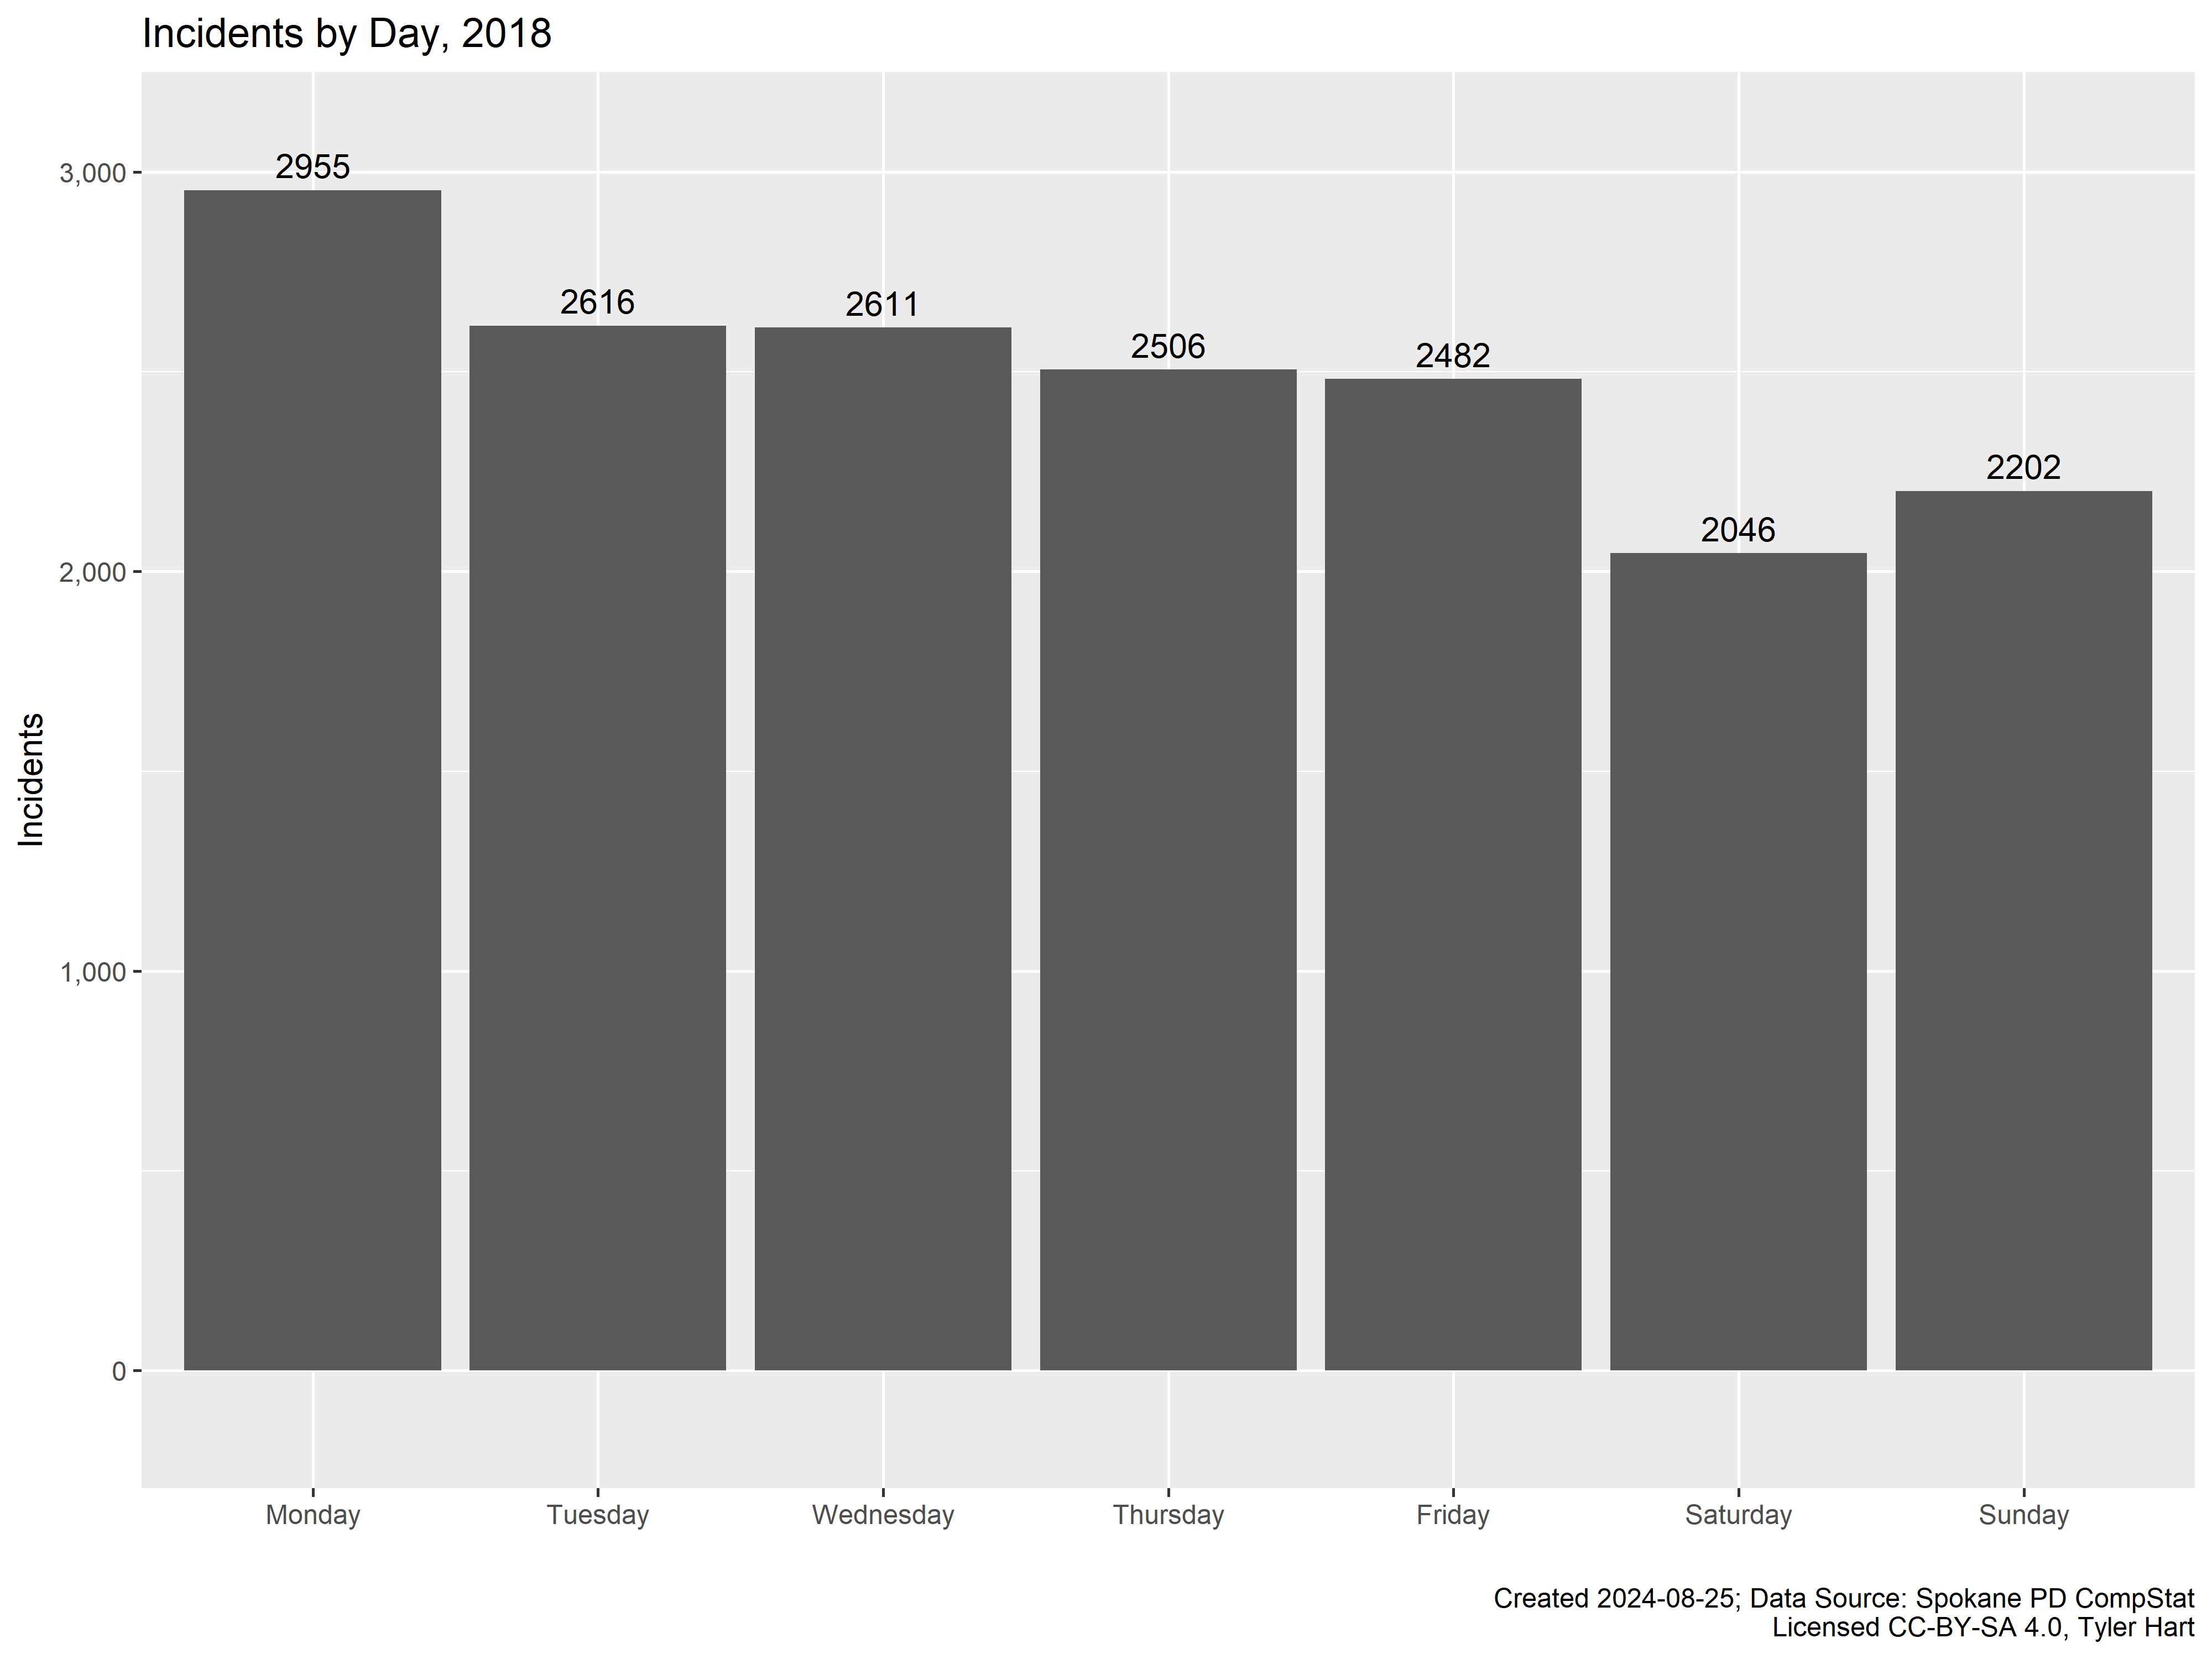
\includegraphics[width=\textwidth]{./figures/plot.2018_offenses_by_weekday-1} \end{center}

\begin{center}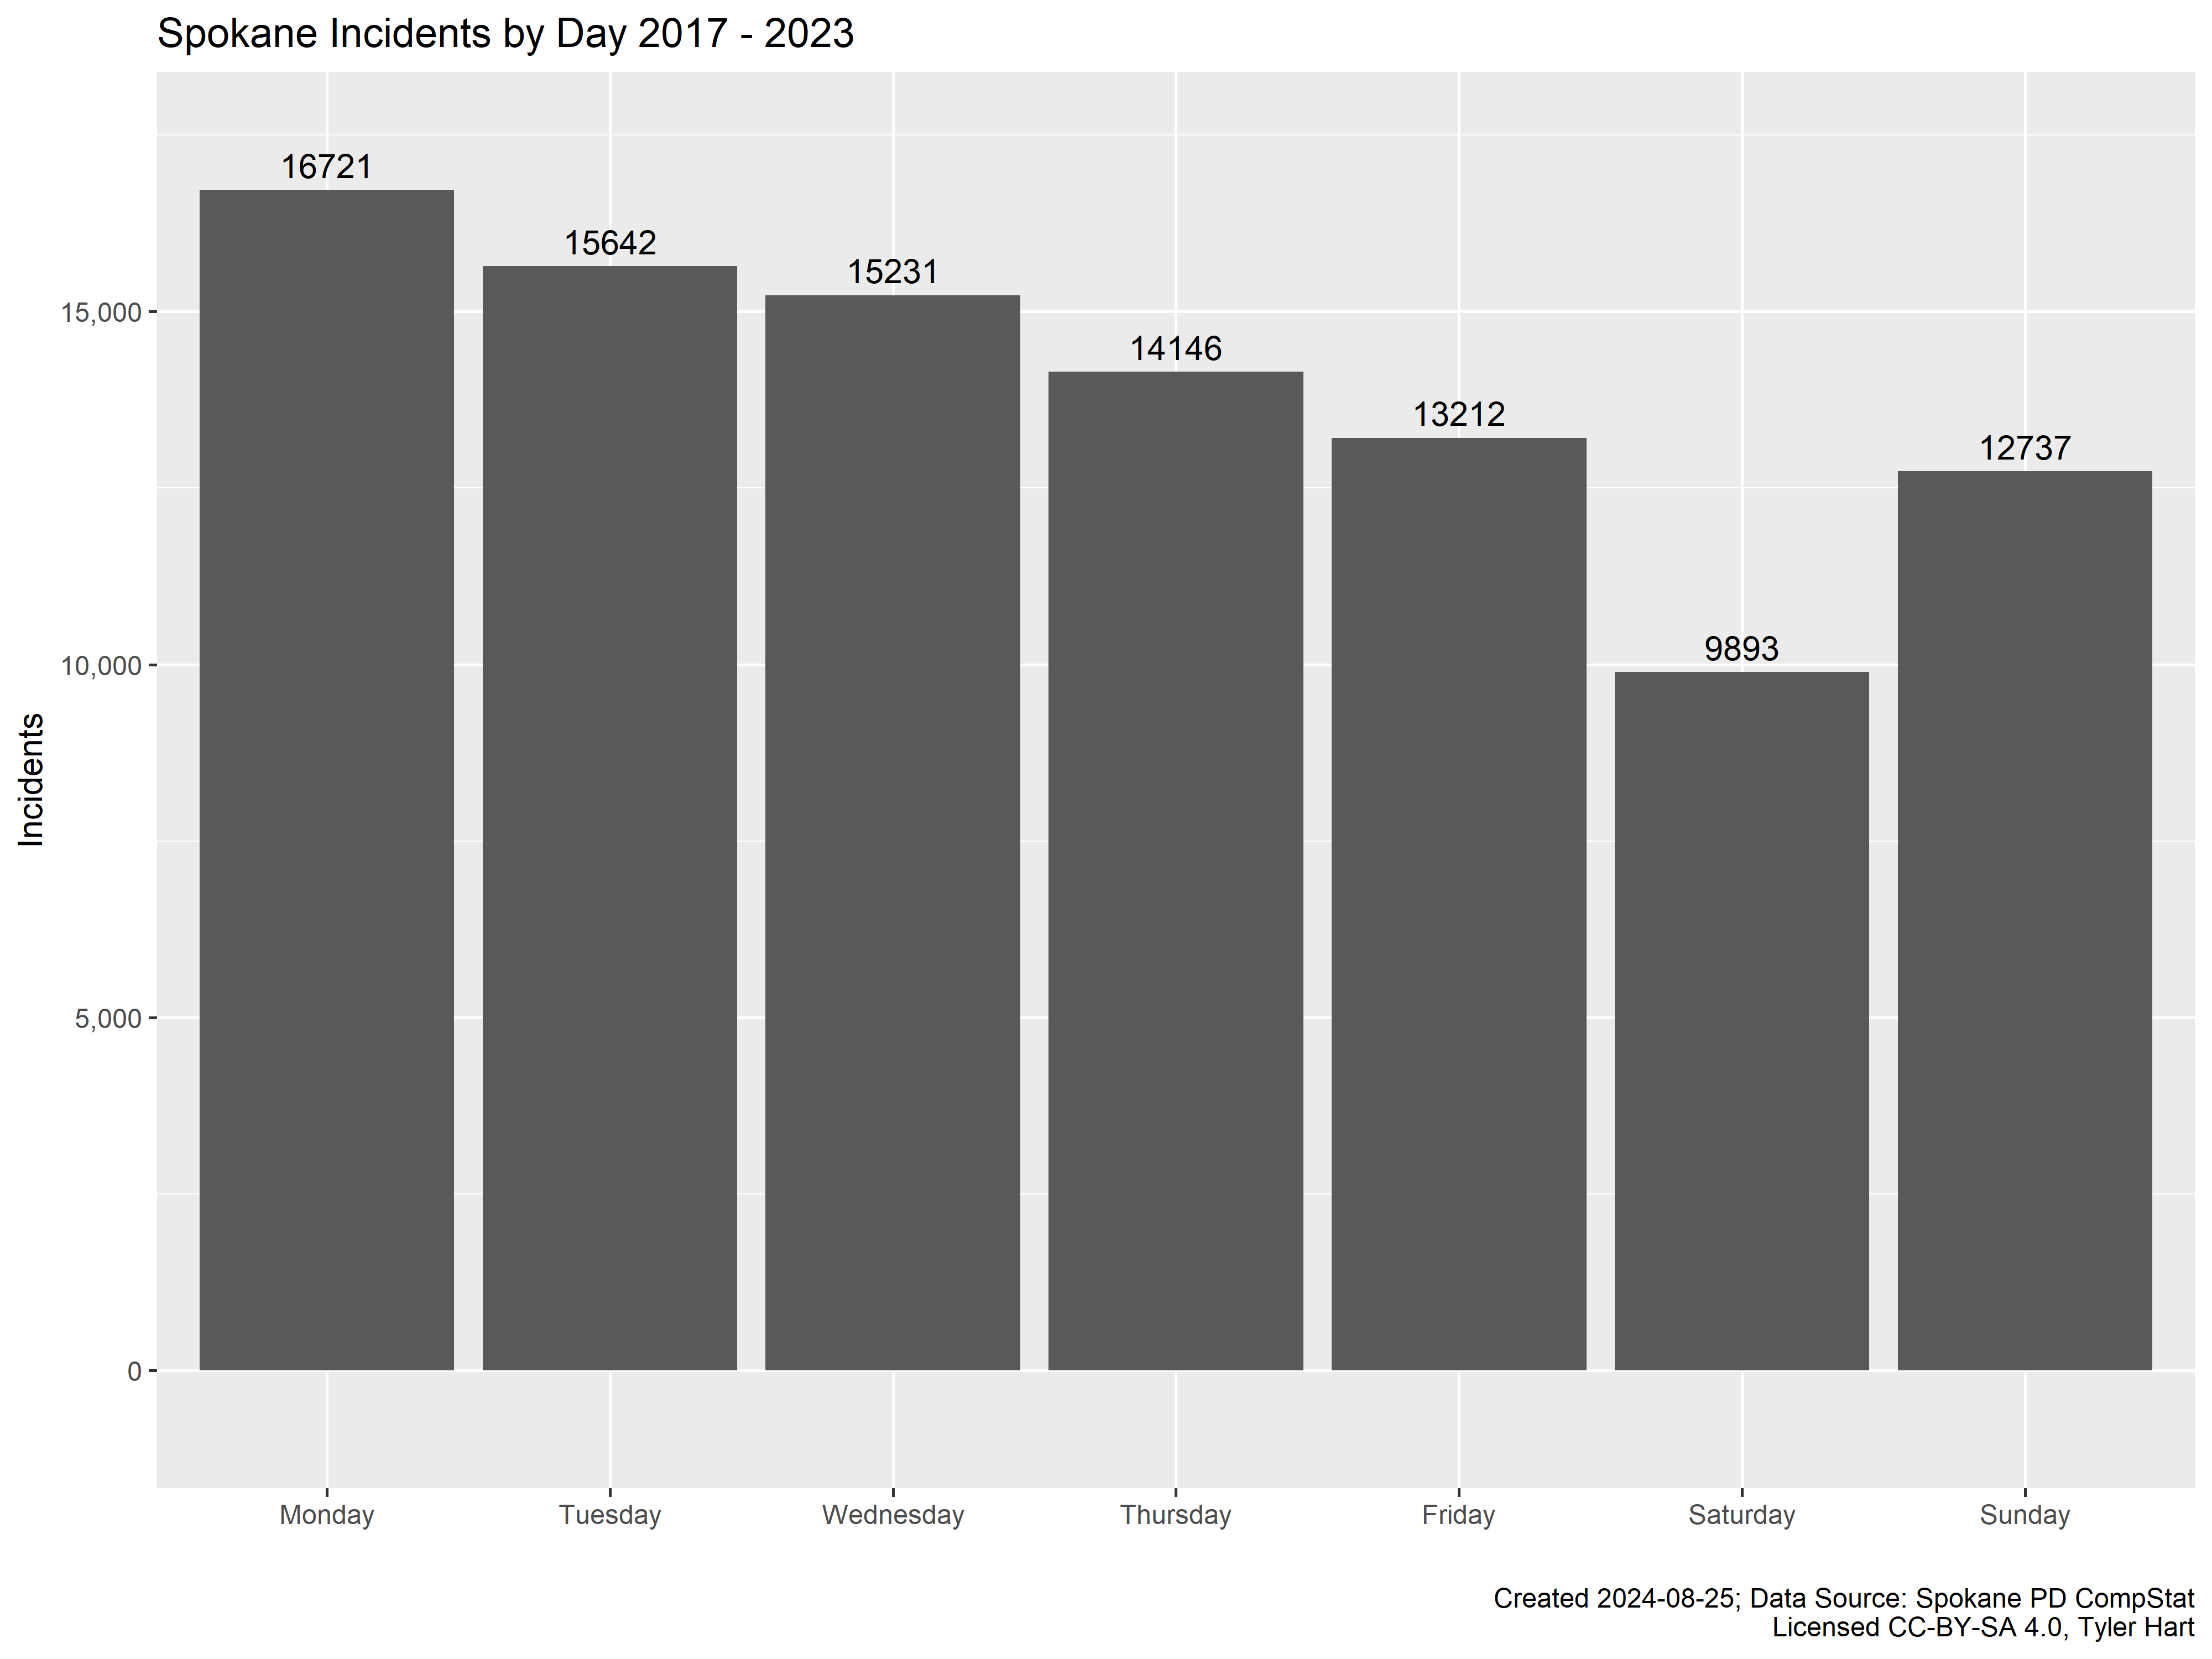
\includegraphics[width=\textwidth]{./figures/plot.Spokane_Offenses_By_Weekday-1} \end{center}

\begin{center}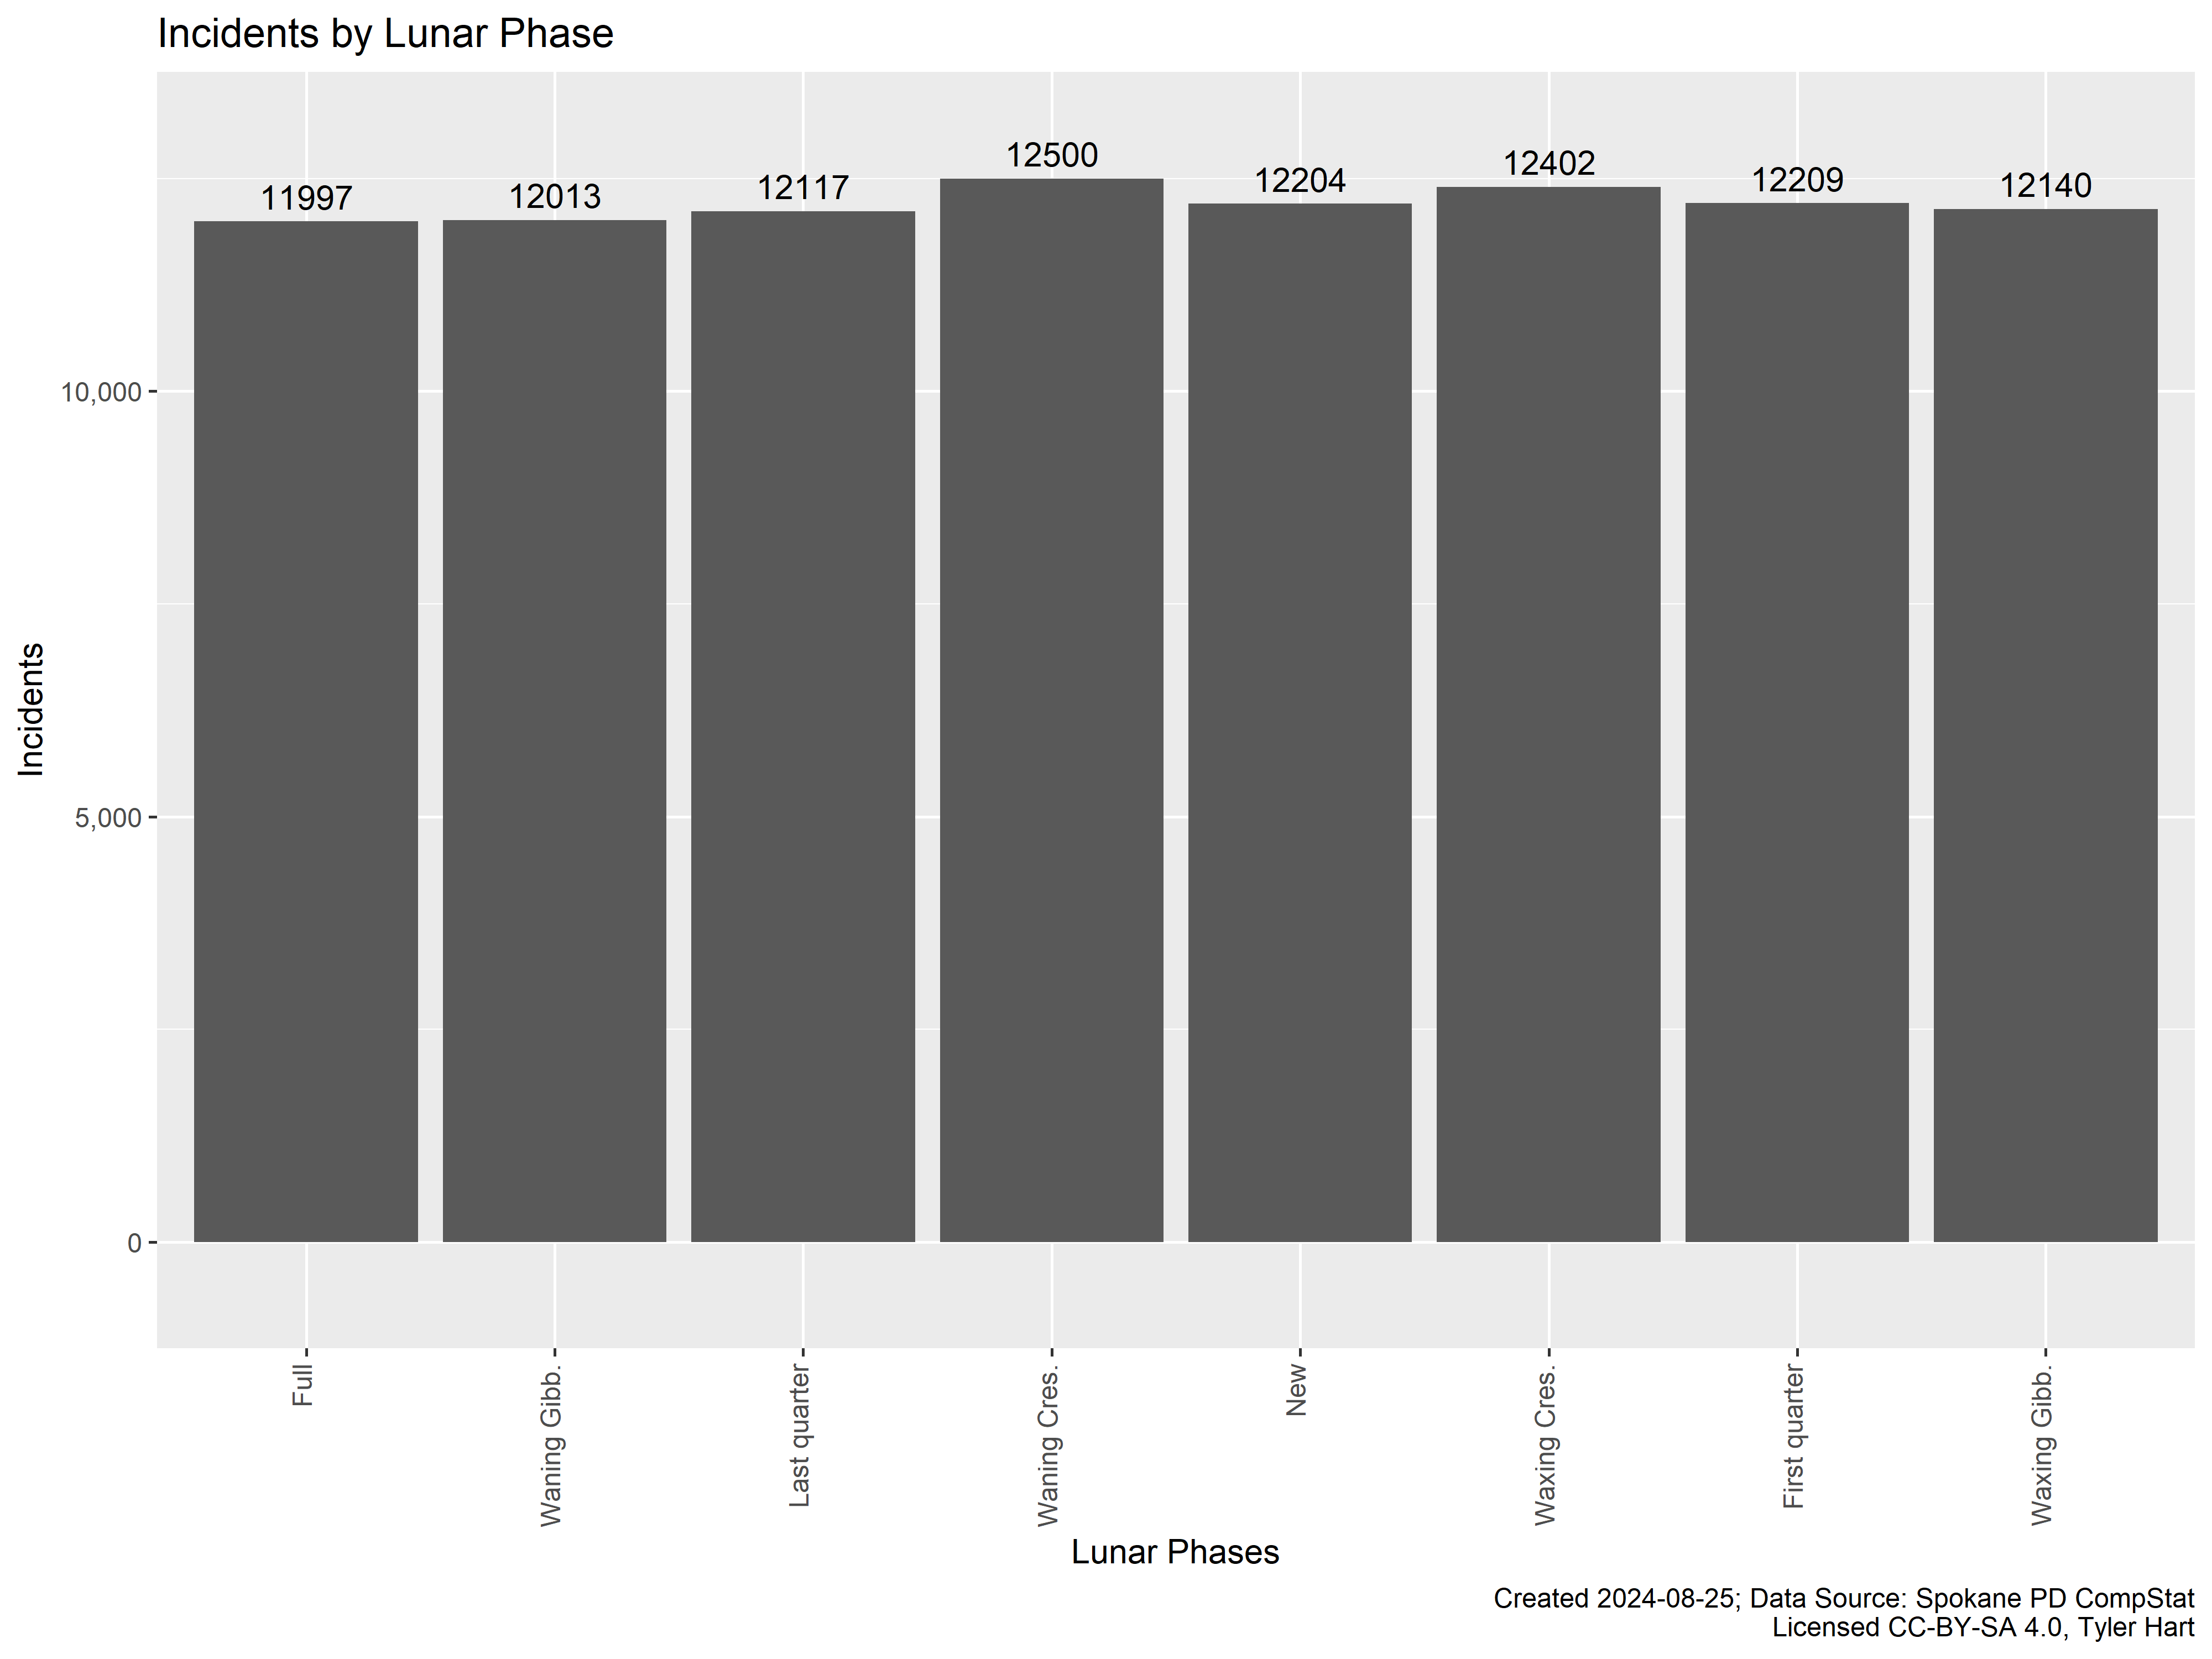
\includegraphics[width=\textwidth]{./figures/plot.offenses_by_lunar_phase-1} \end{center}

\begin{center}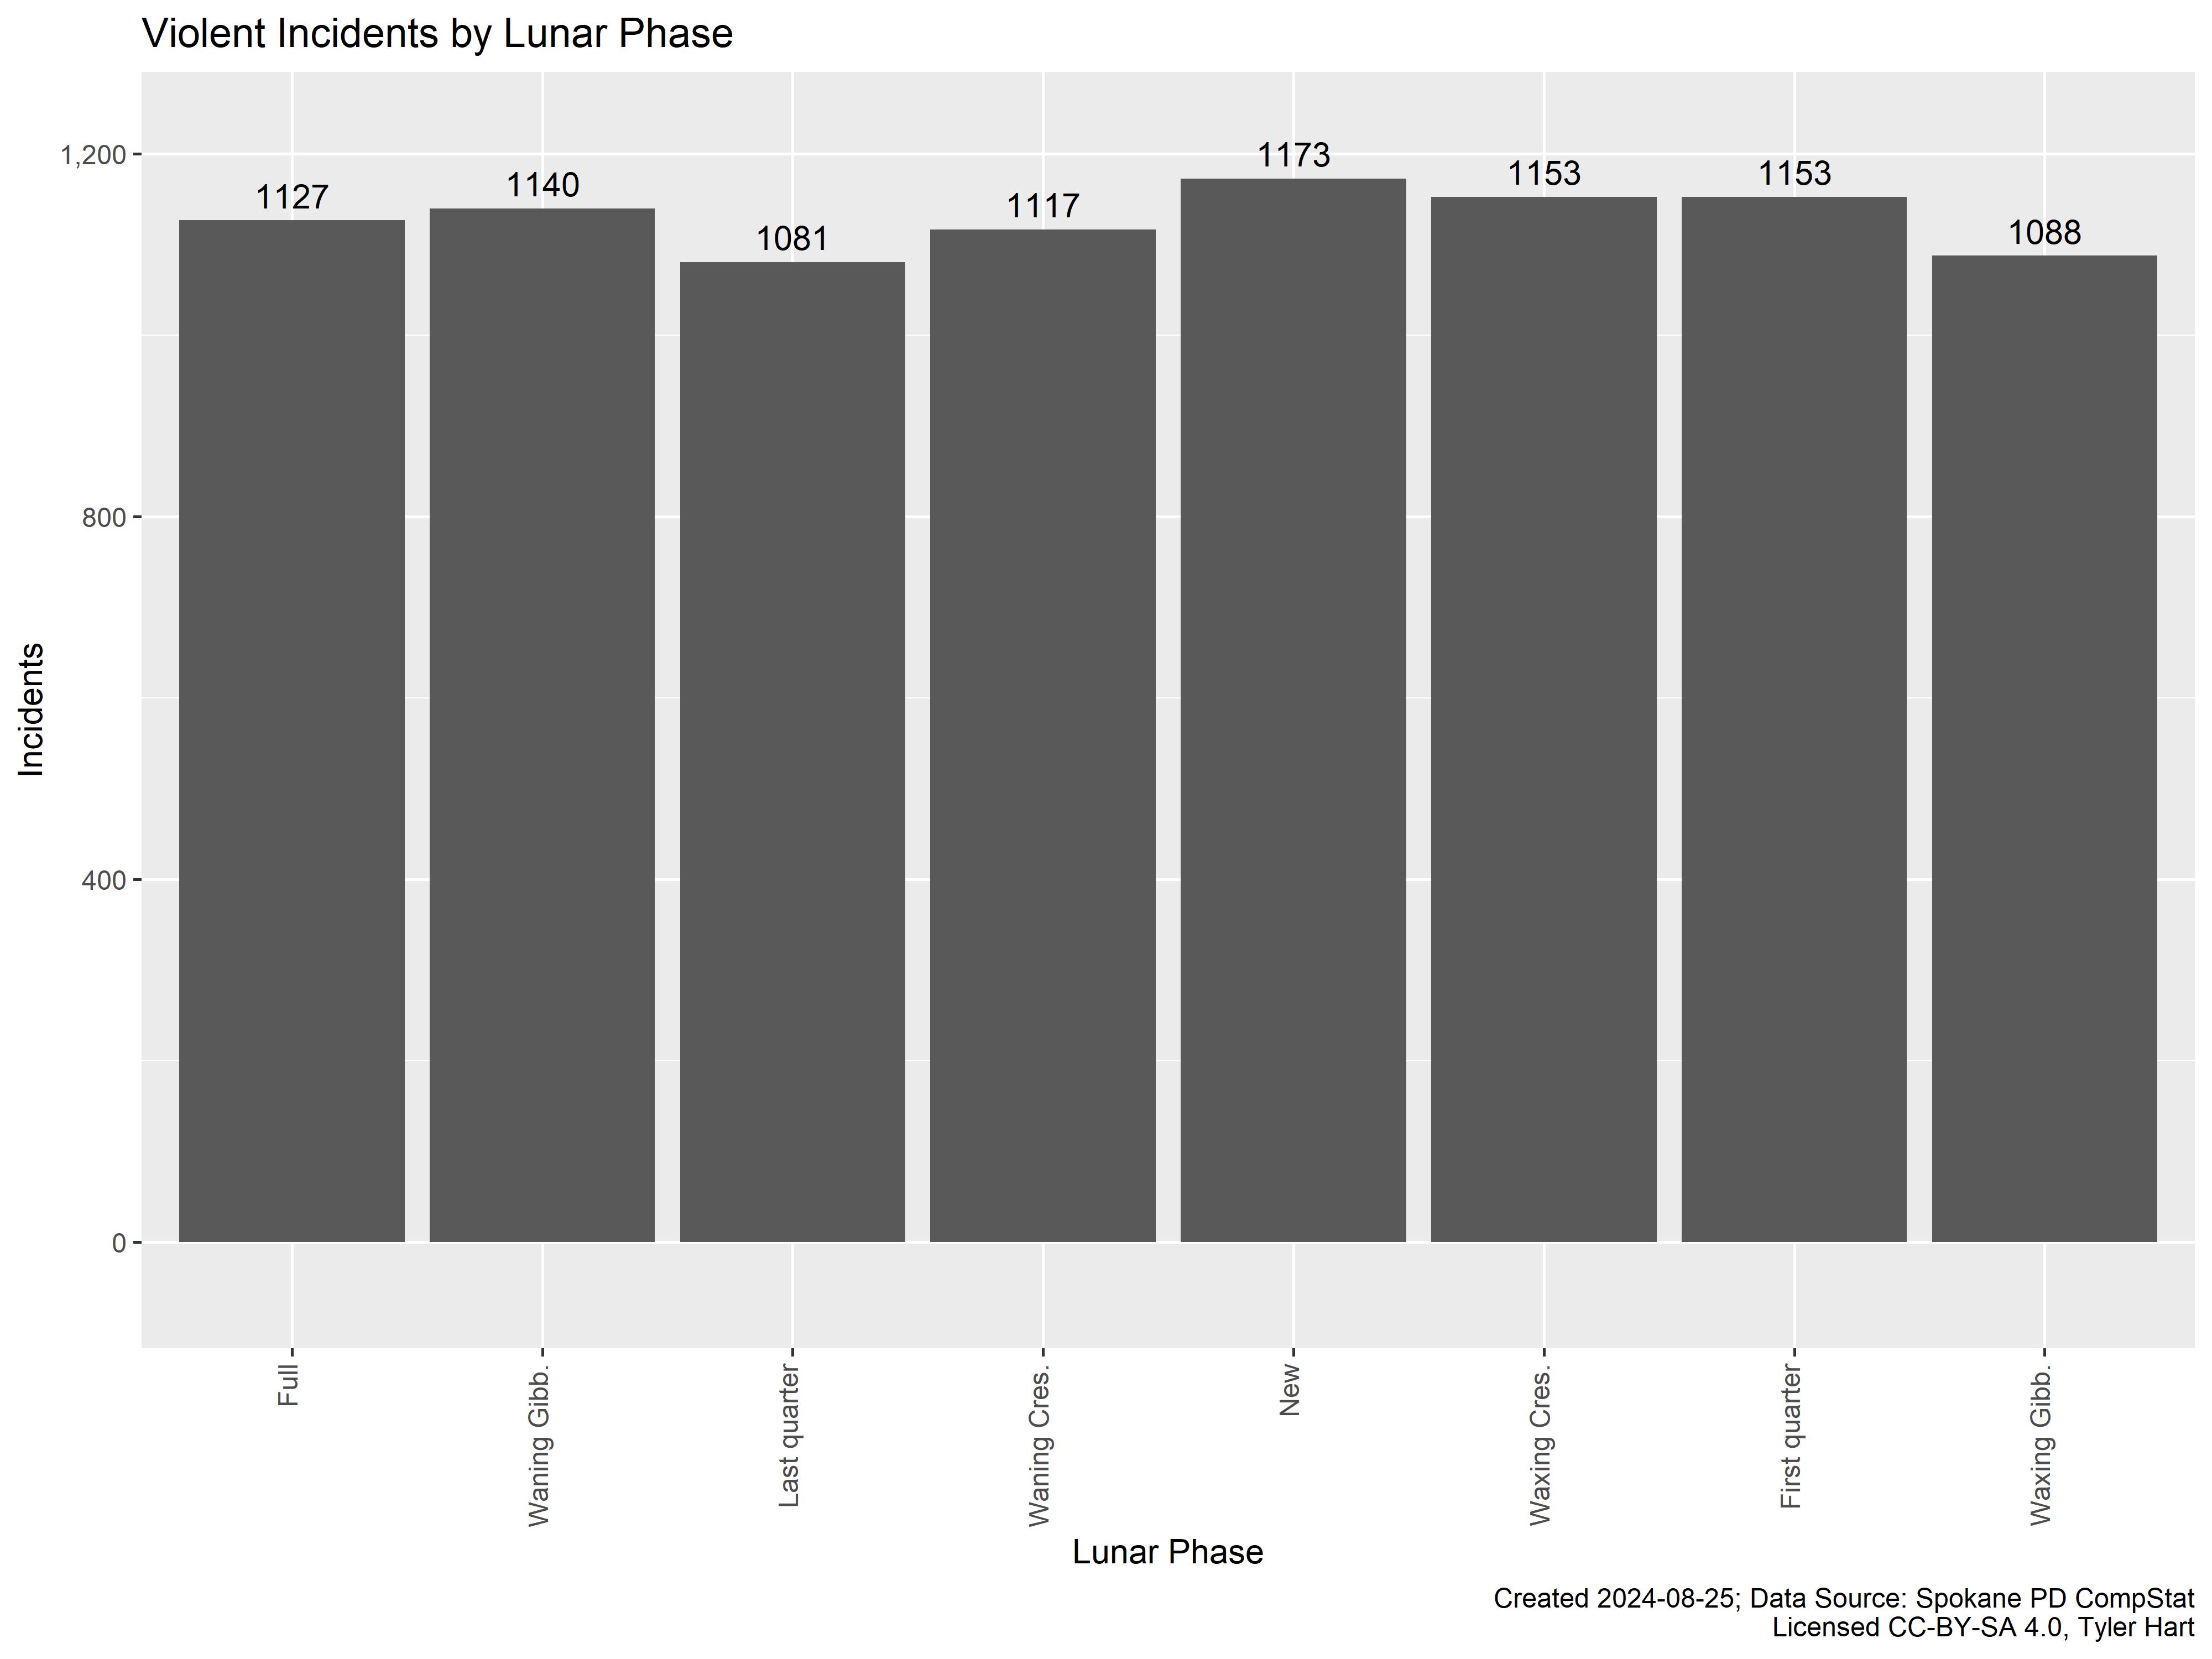
\includegraphics[width=\textwidth]{./figures/plot.violent_offenses_by_lunar_phase-1} \end{center}

\hypertarget{seasonal}{%
\section{Seasonal}\label{seasonal}}

\hypertarget{assault}{%
\subsection{Assault}\label{assault}}

\begin{center}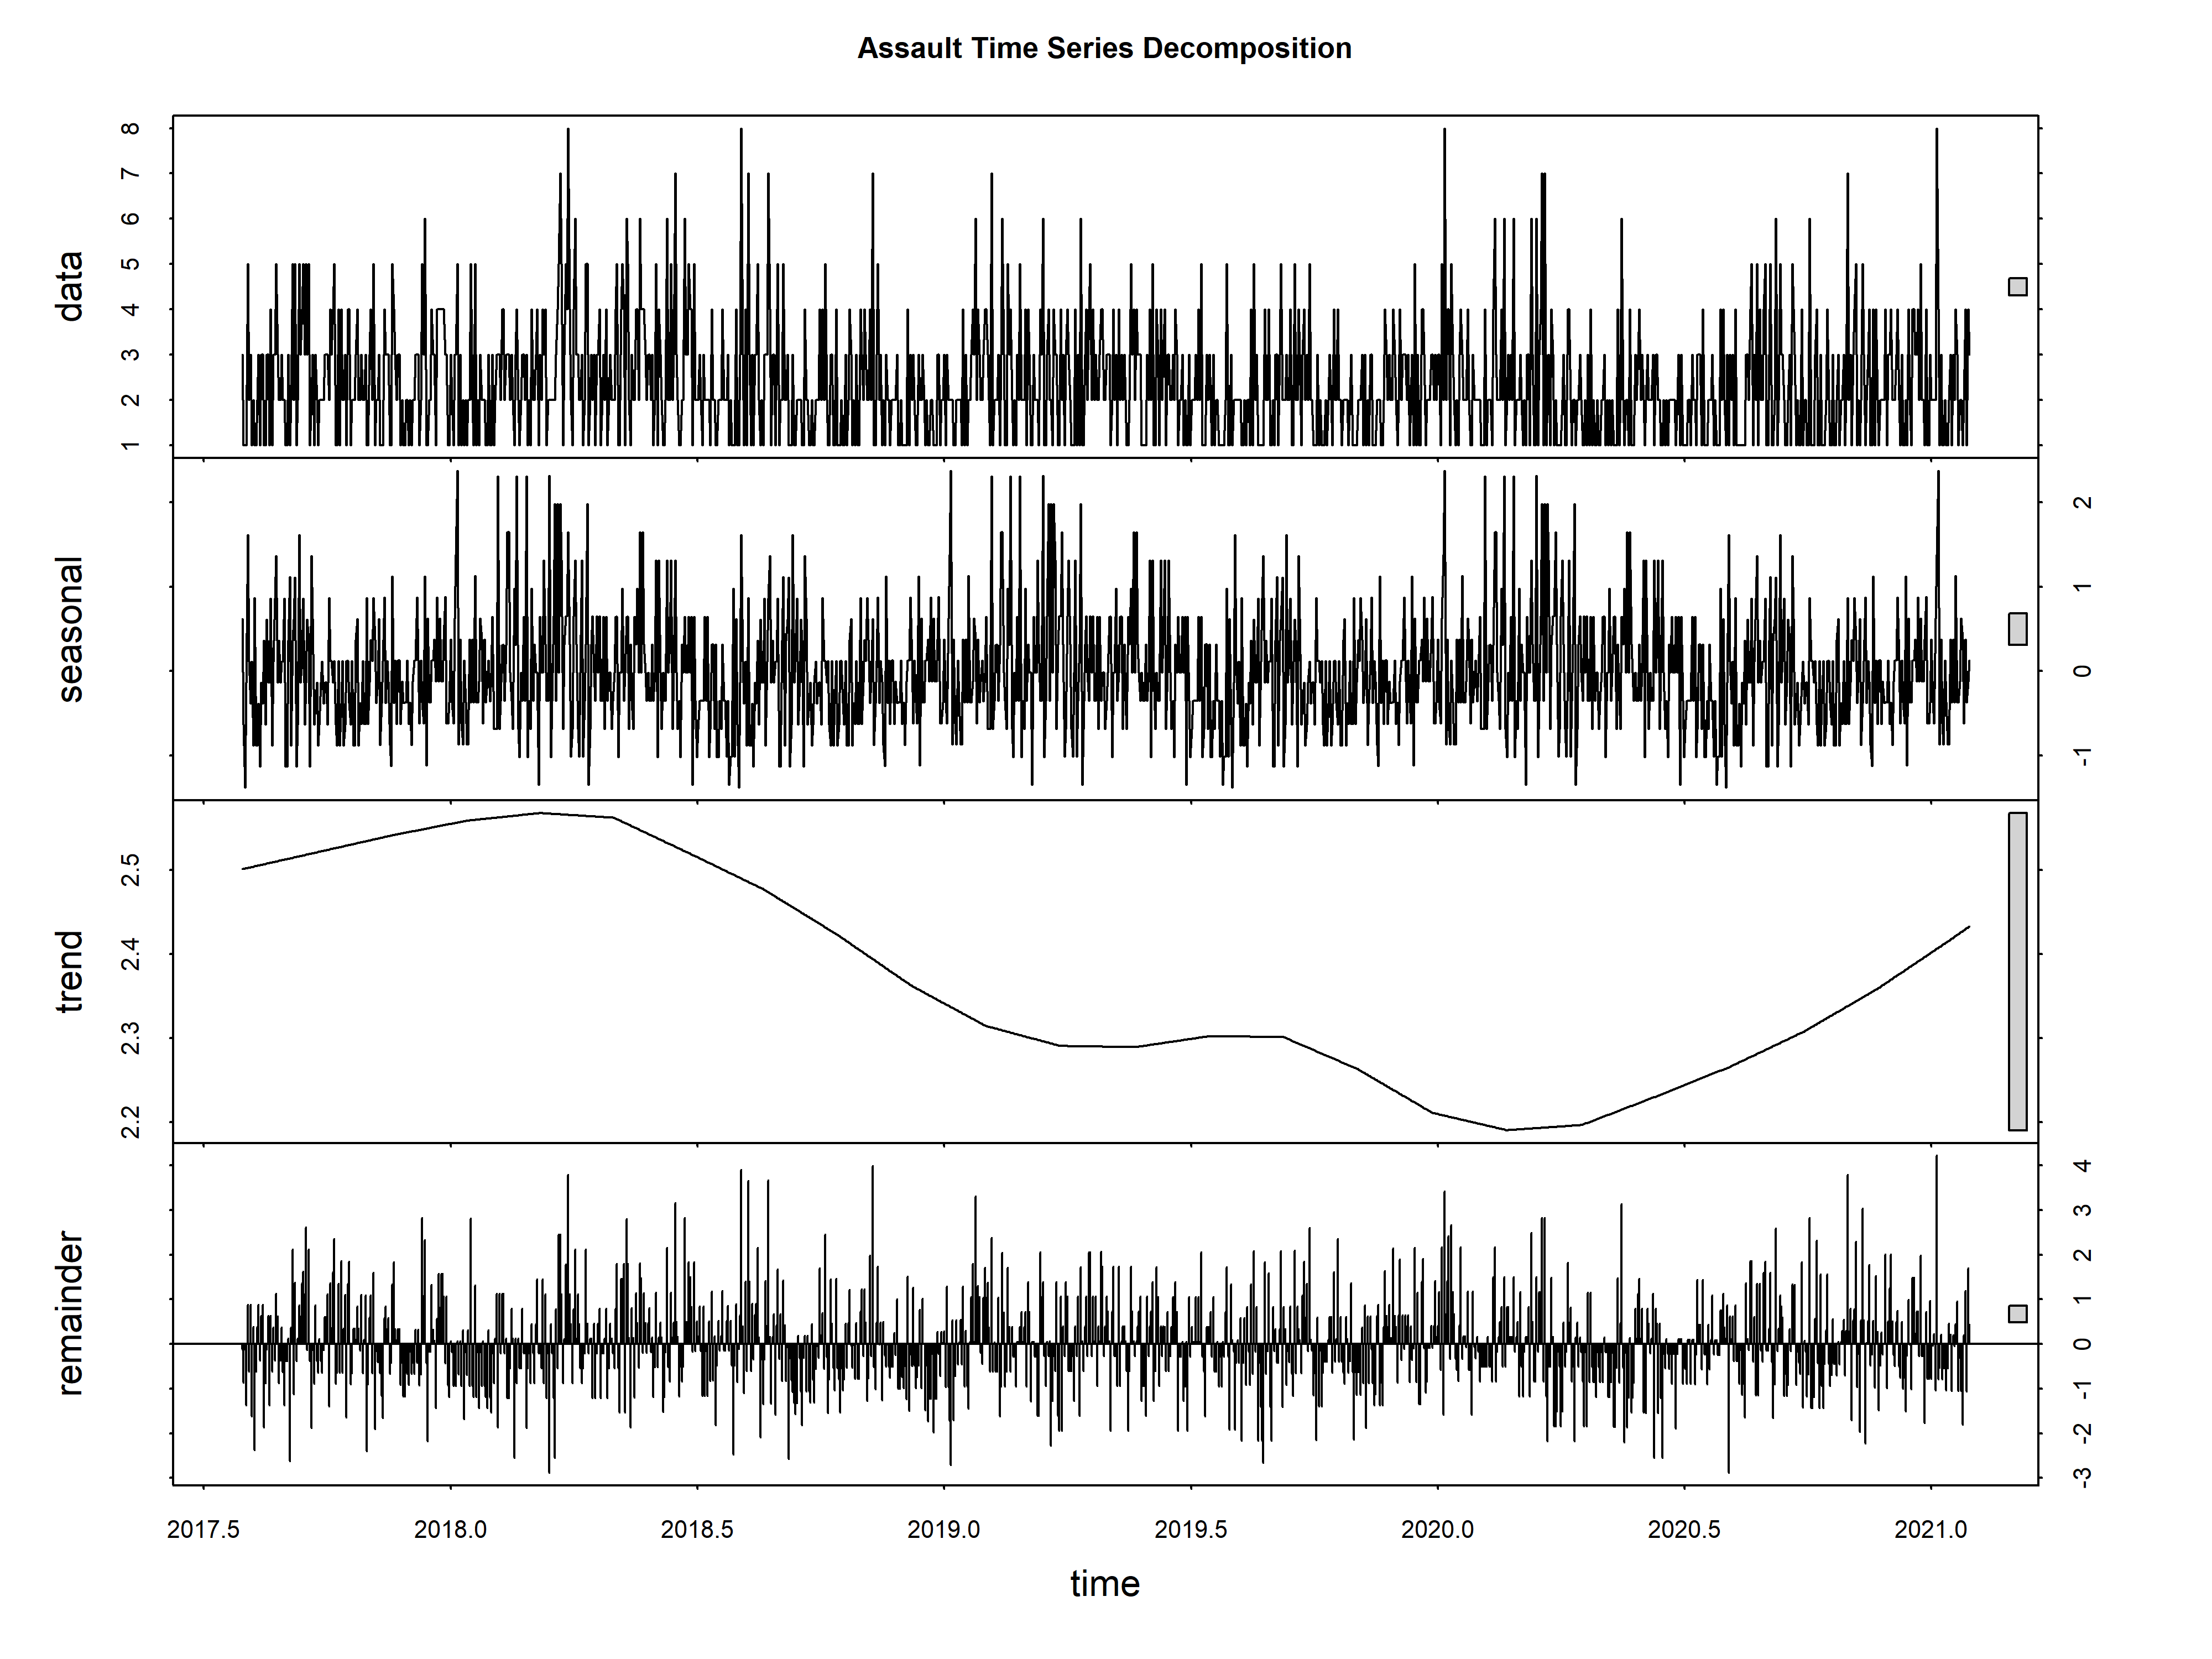
\includegraphics[width=\textwidth]{./figures/plot.assault_time_series_decomposition-1} \end{center}

\hypertarget{arson}{%
\subsection{Arson}\label{arson}}

\begin{center}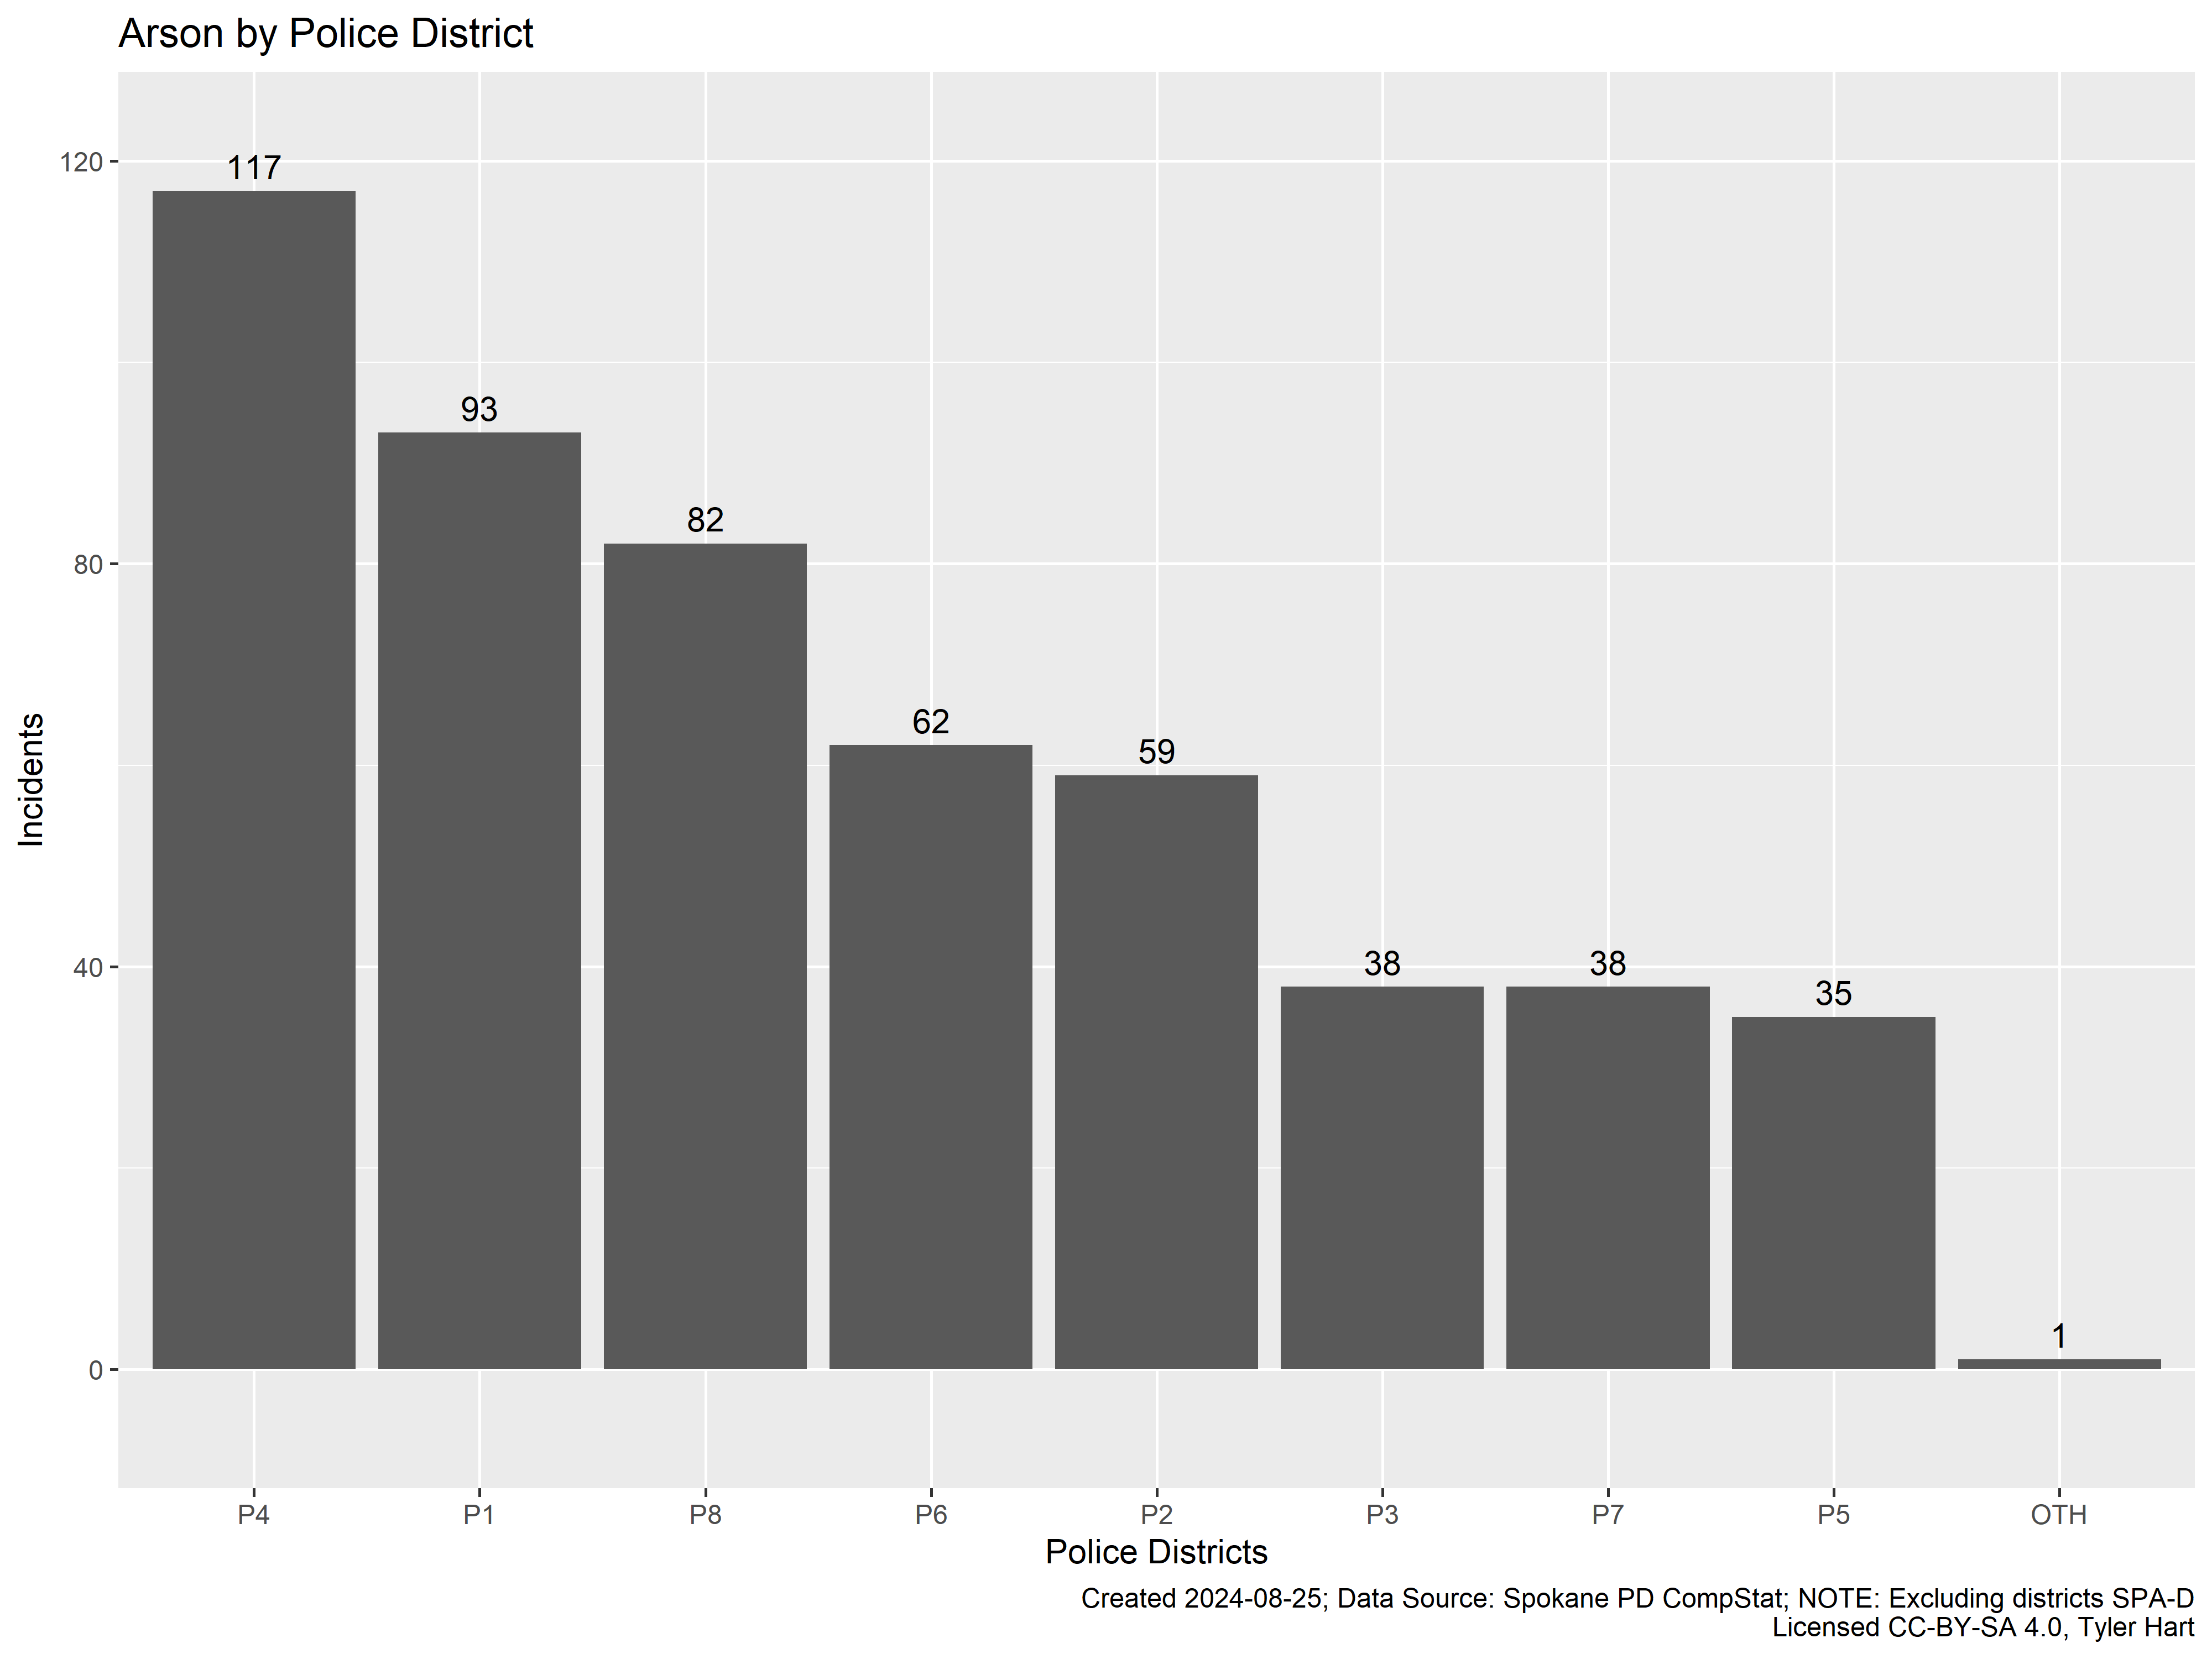
\includegraphics[width=\textwidth]{./figures/plot.arson_by_district-1} \end{center}

\hypertarget{burglary}{%
\subsection{Burglary}\label{burglary}}

\begin{center}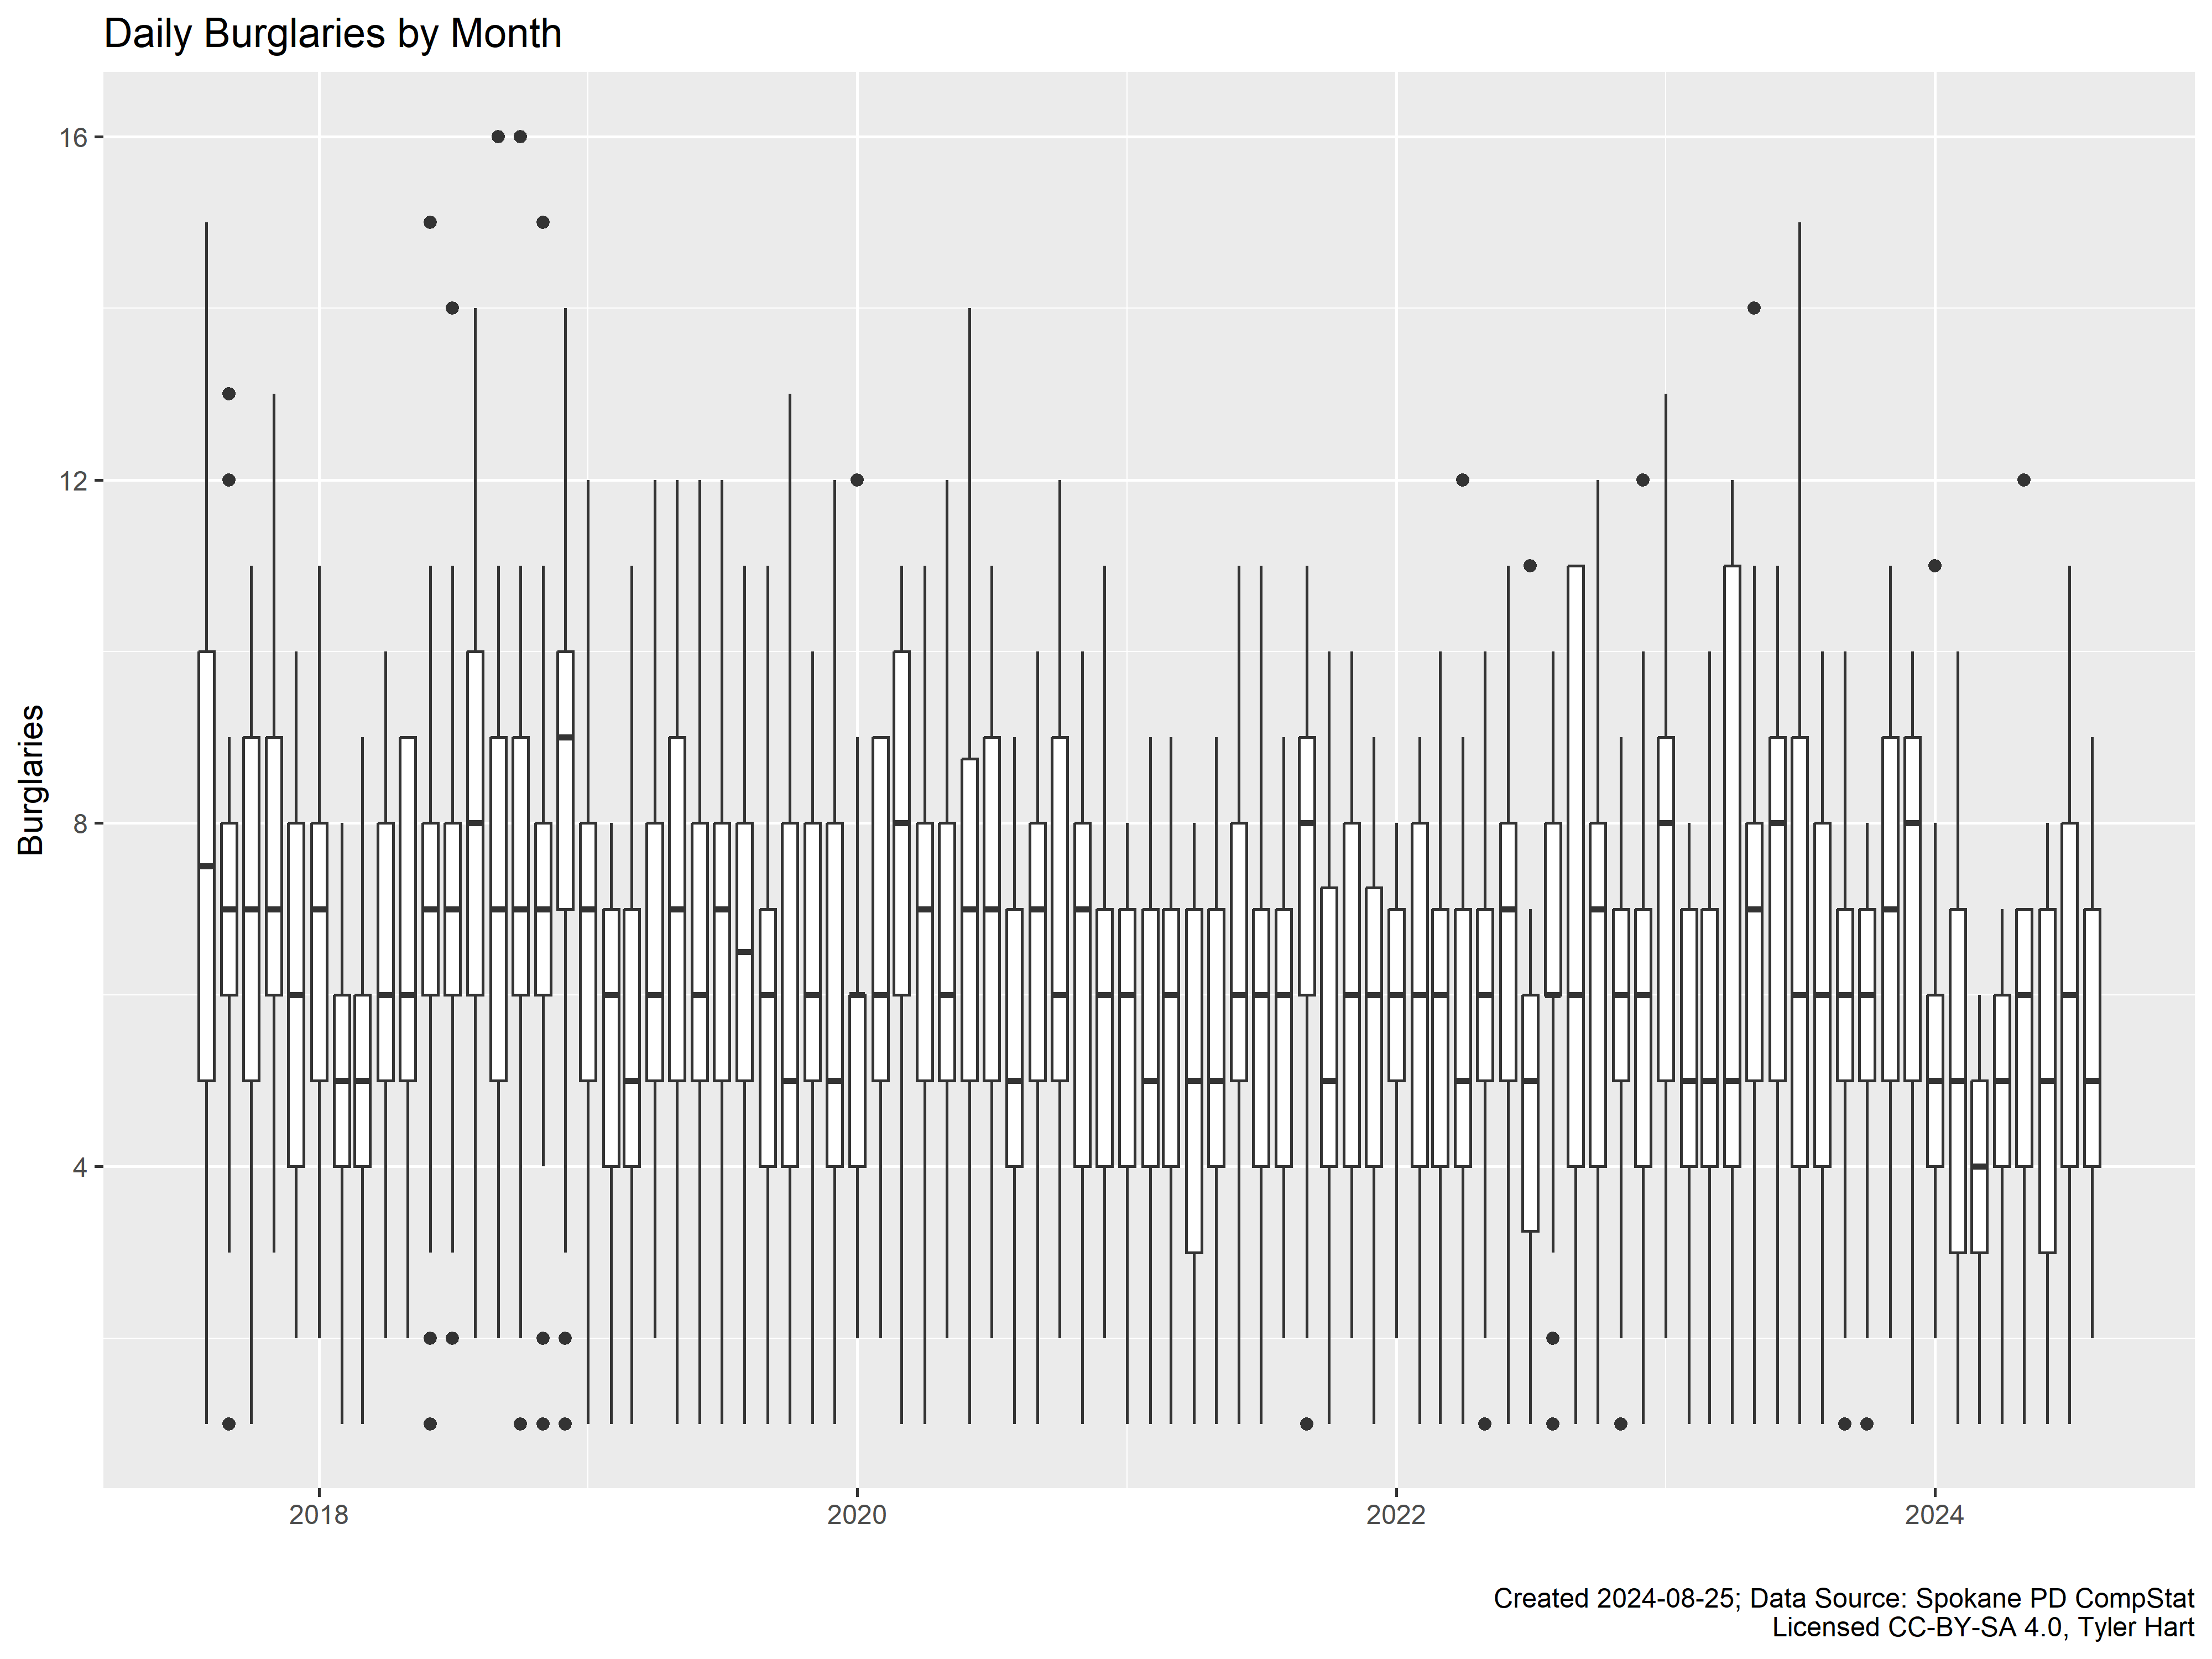
\includegraphics[width=\textwidth]{./figures/plot.boxplot_avg_daily_burglaries_by_month-1} \end{center}

\begin{center}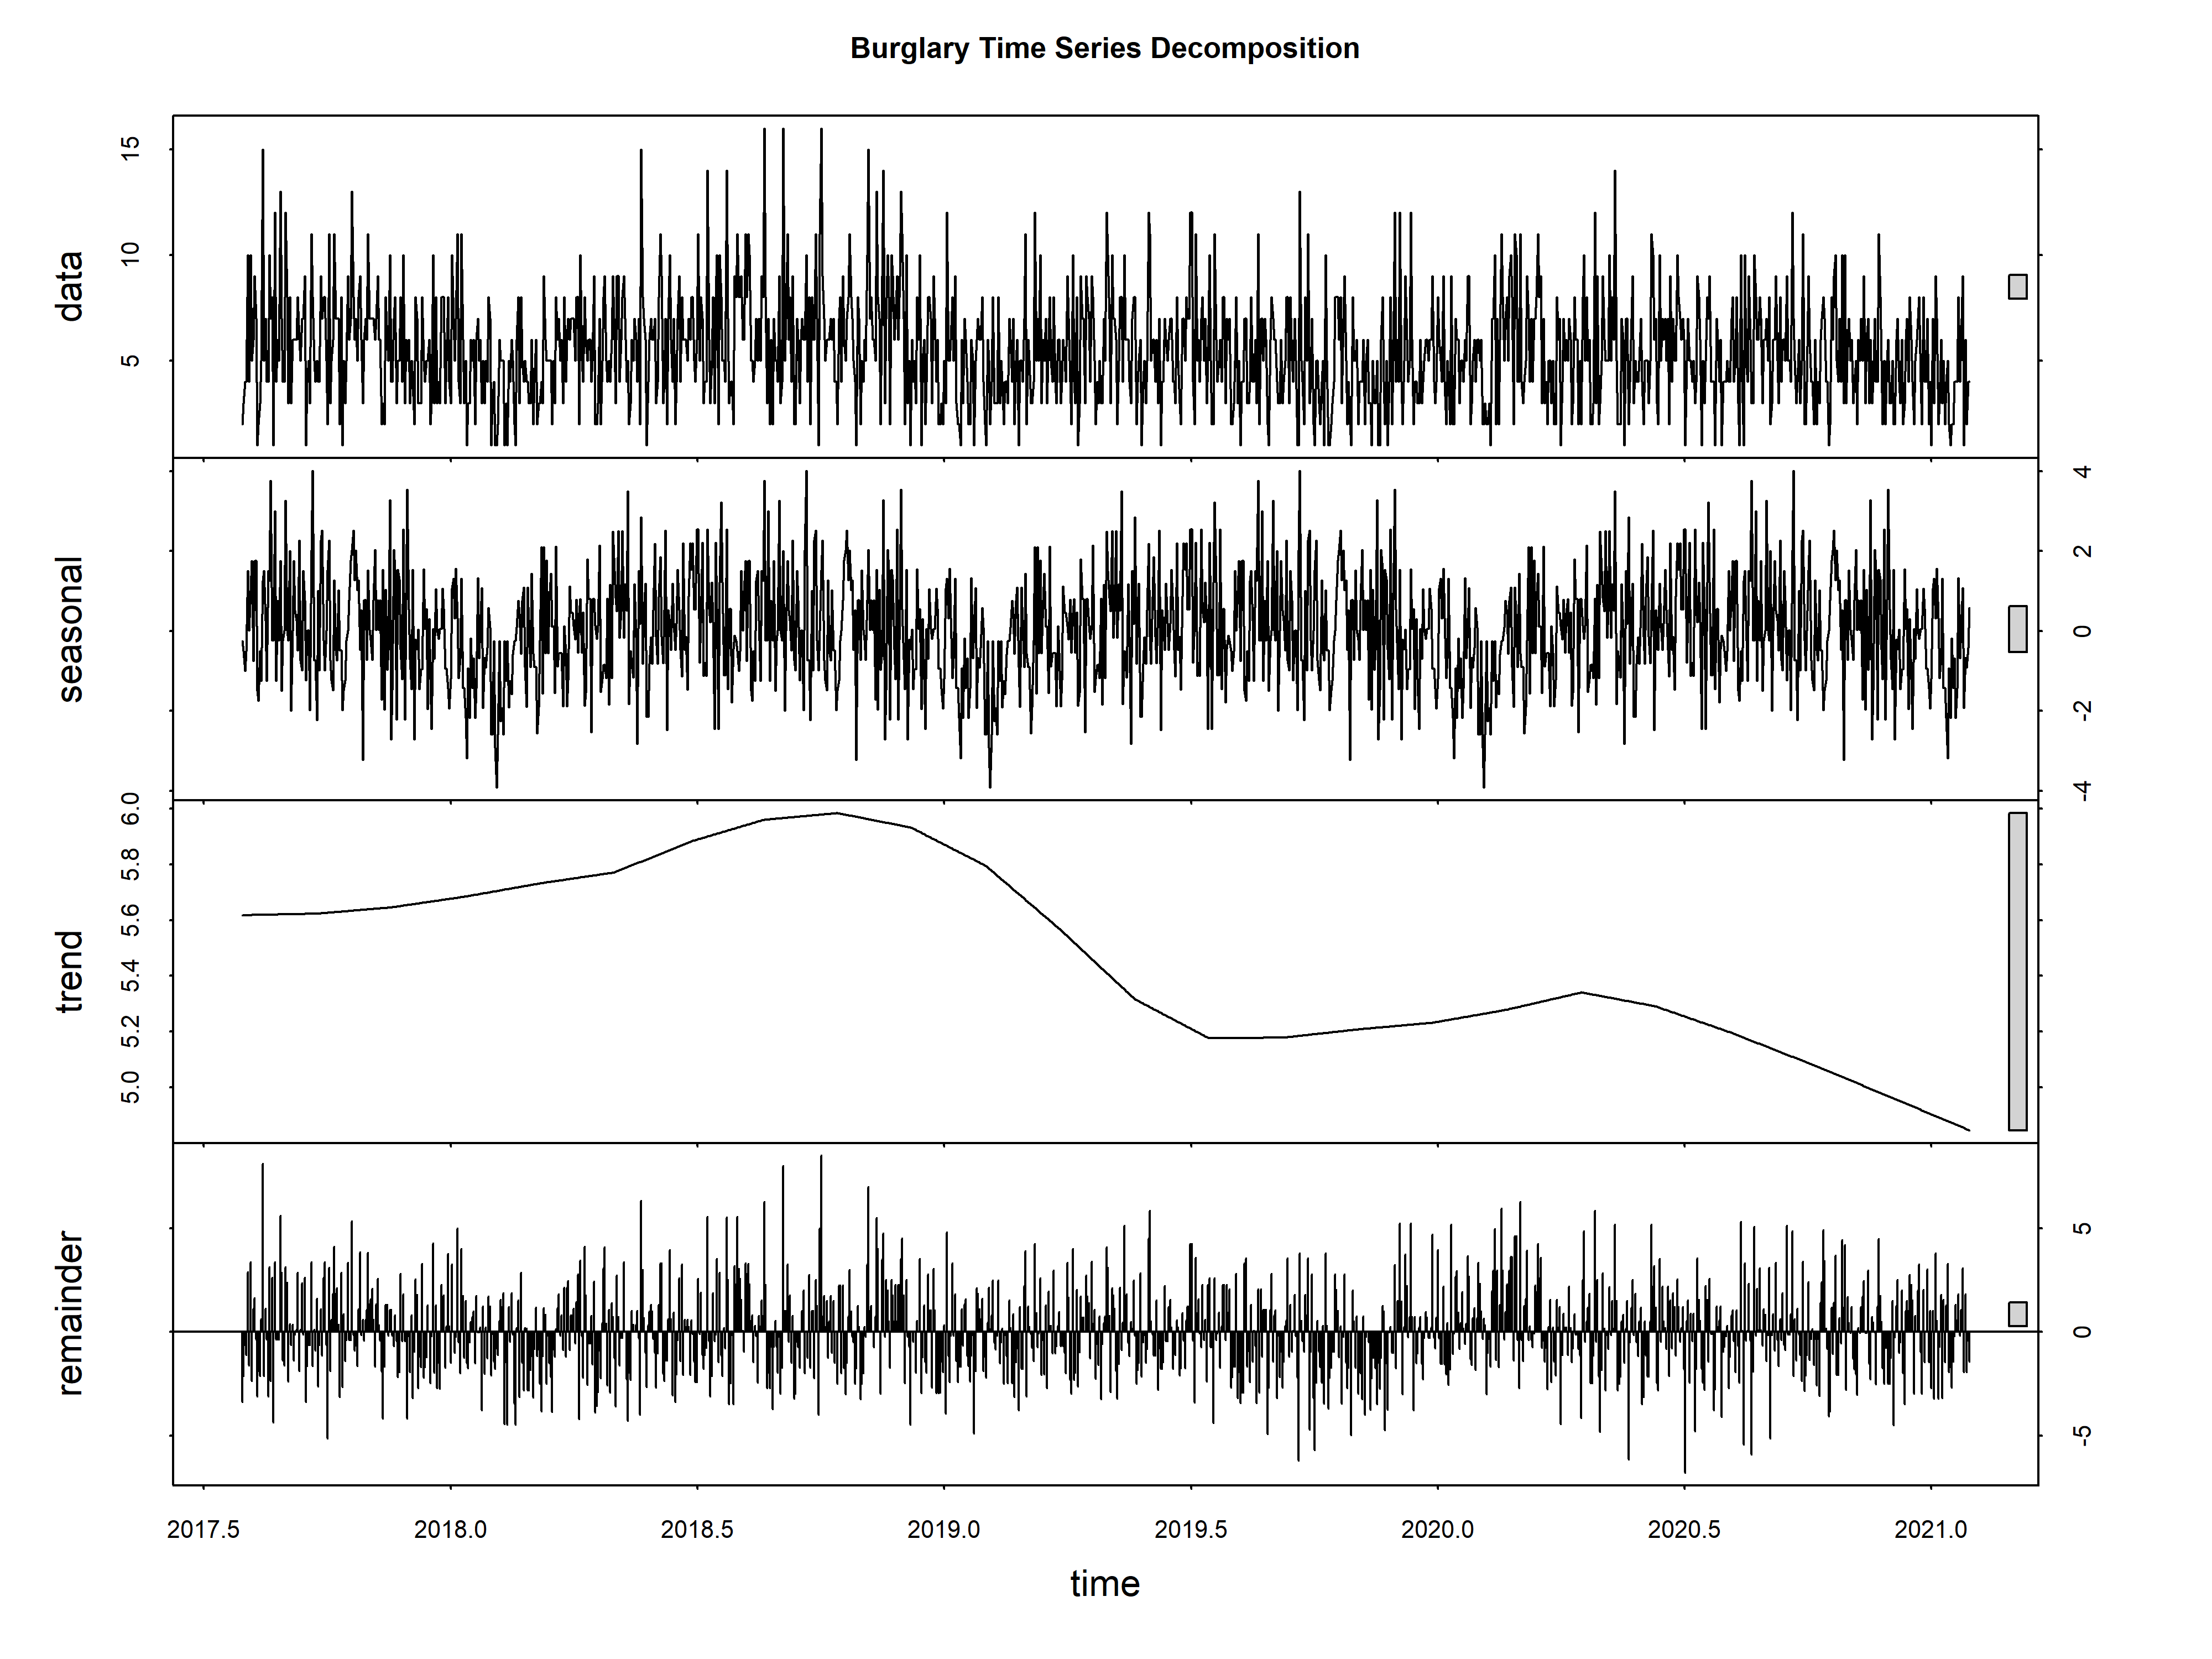
\includegraphics[width=\textwidth]{./figures/plot.burglary_time_series_decomposition-1} \end{center}

\hypertarget{theft}{%
\subsection{Theft}\label{theft}}

\begin{center}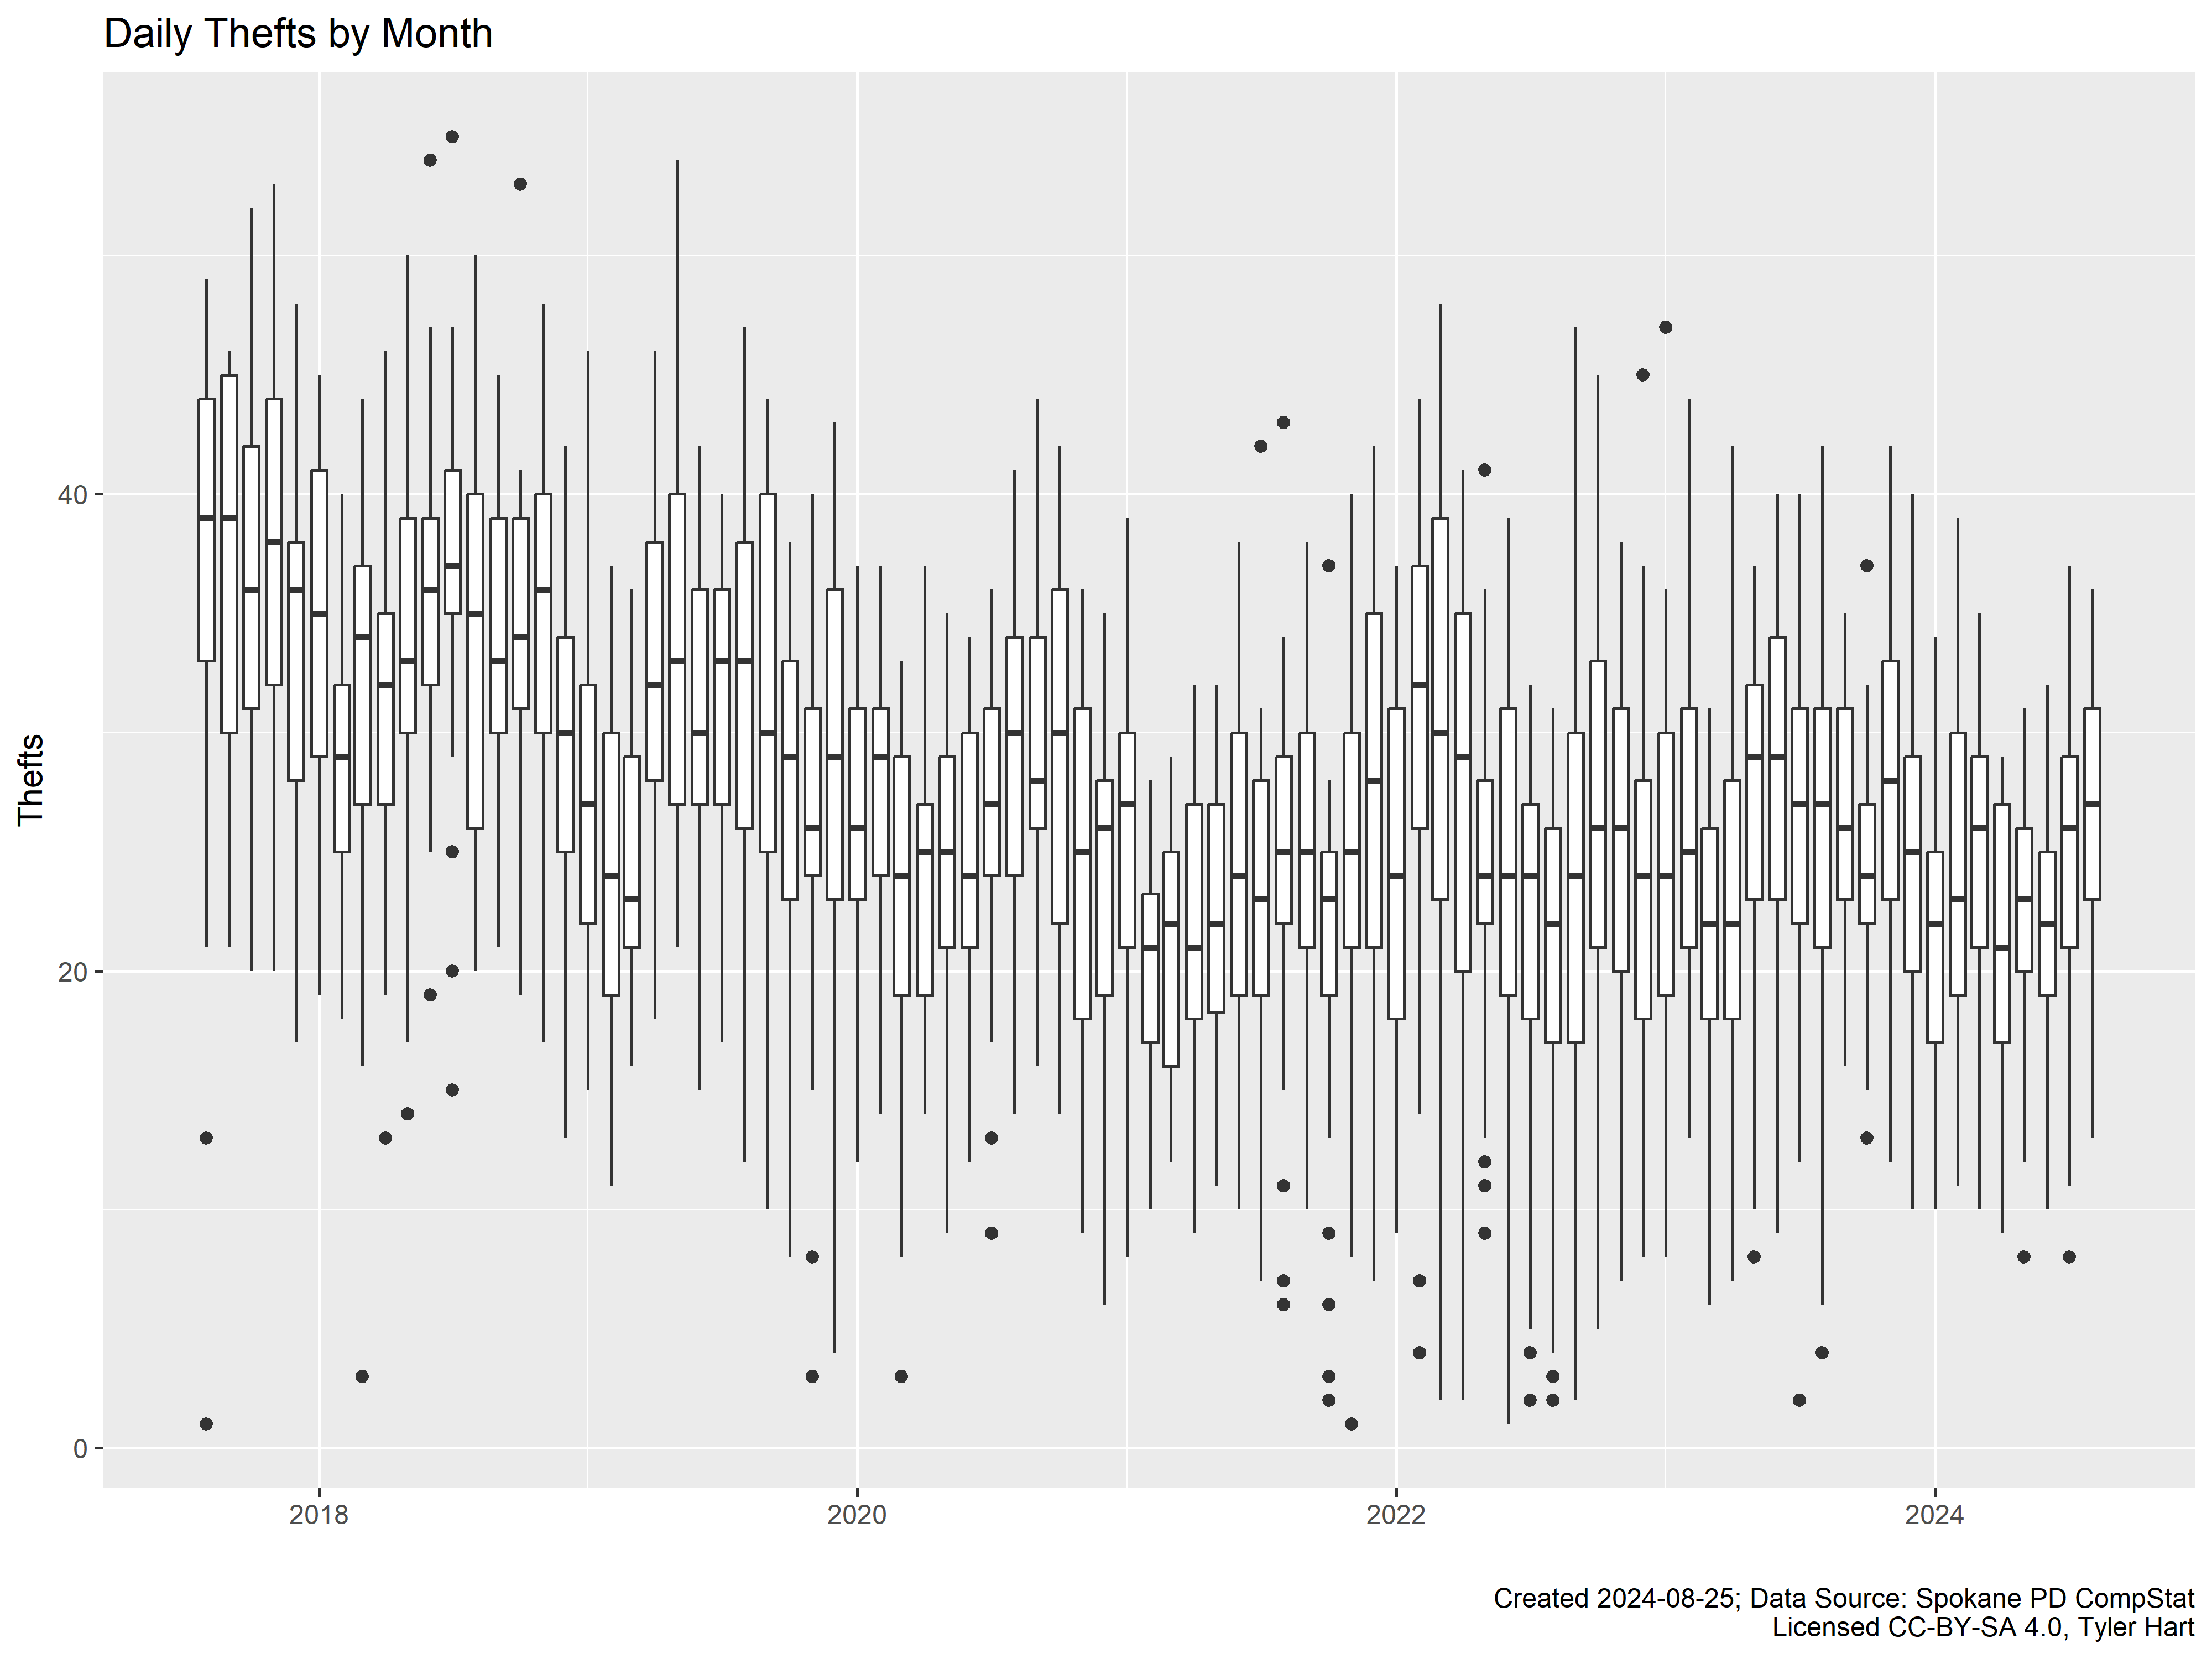
\includegraphics[width=\textwidth]{./figures/plot.boxplot_avg_daily_thefts_by_month-1} \end{center}

\begin{center}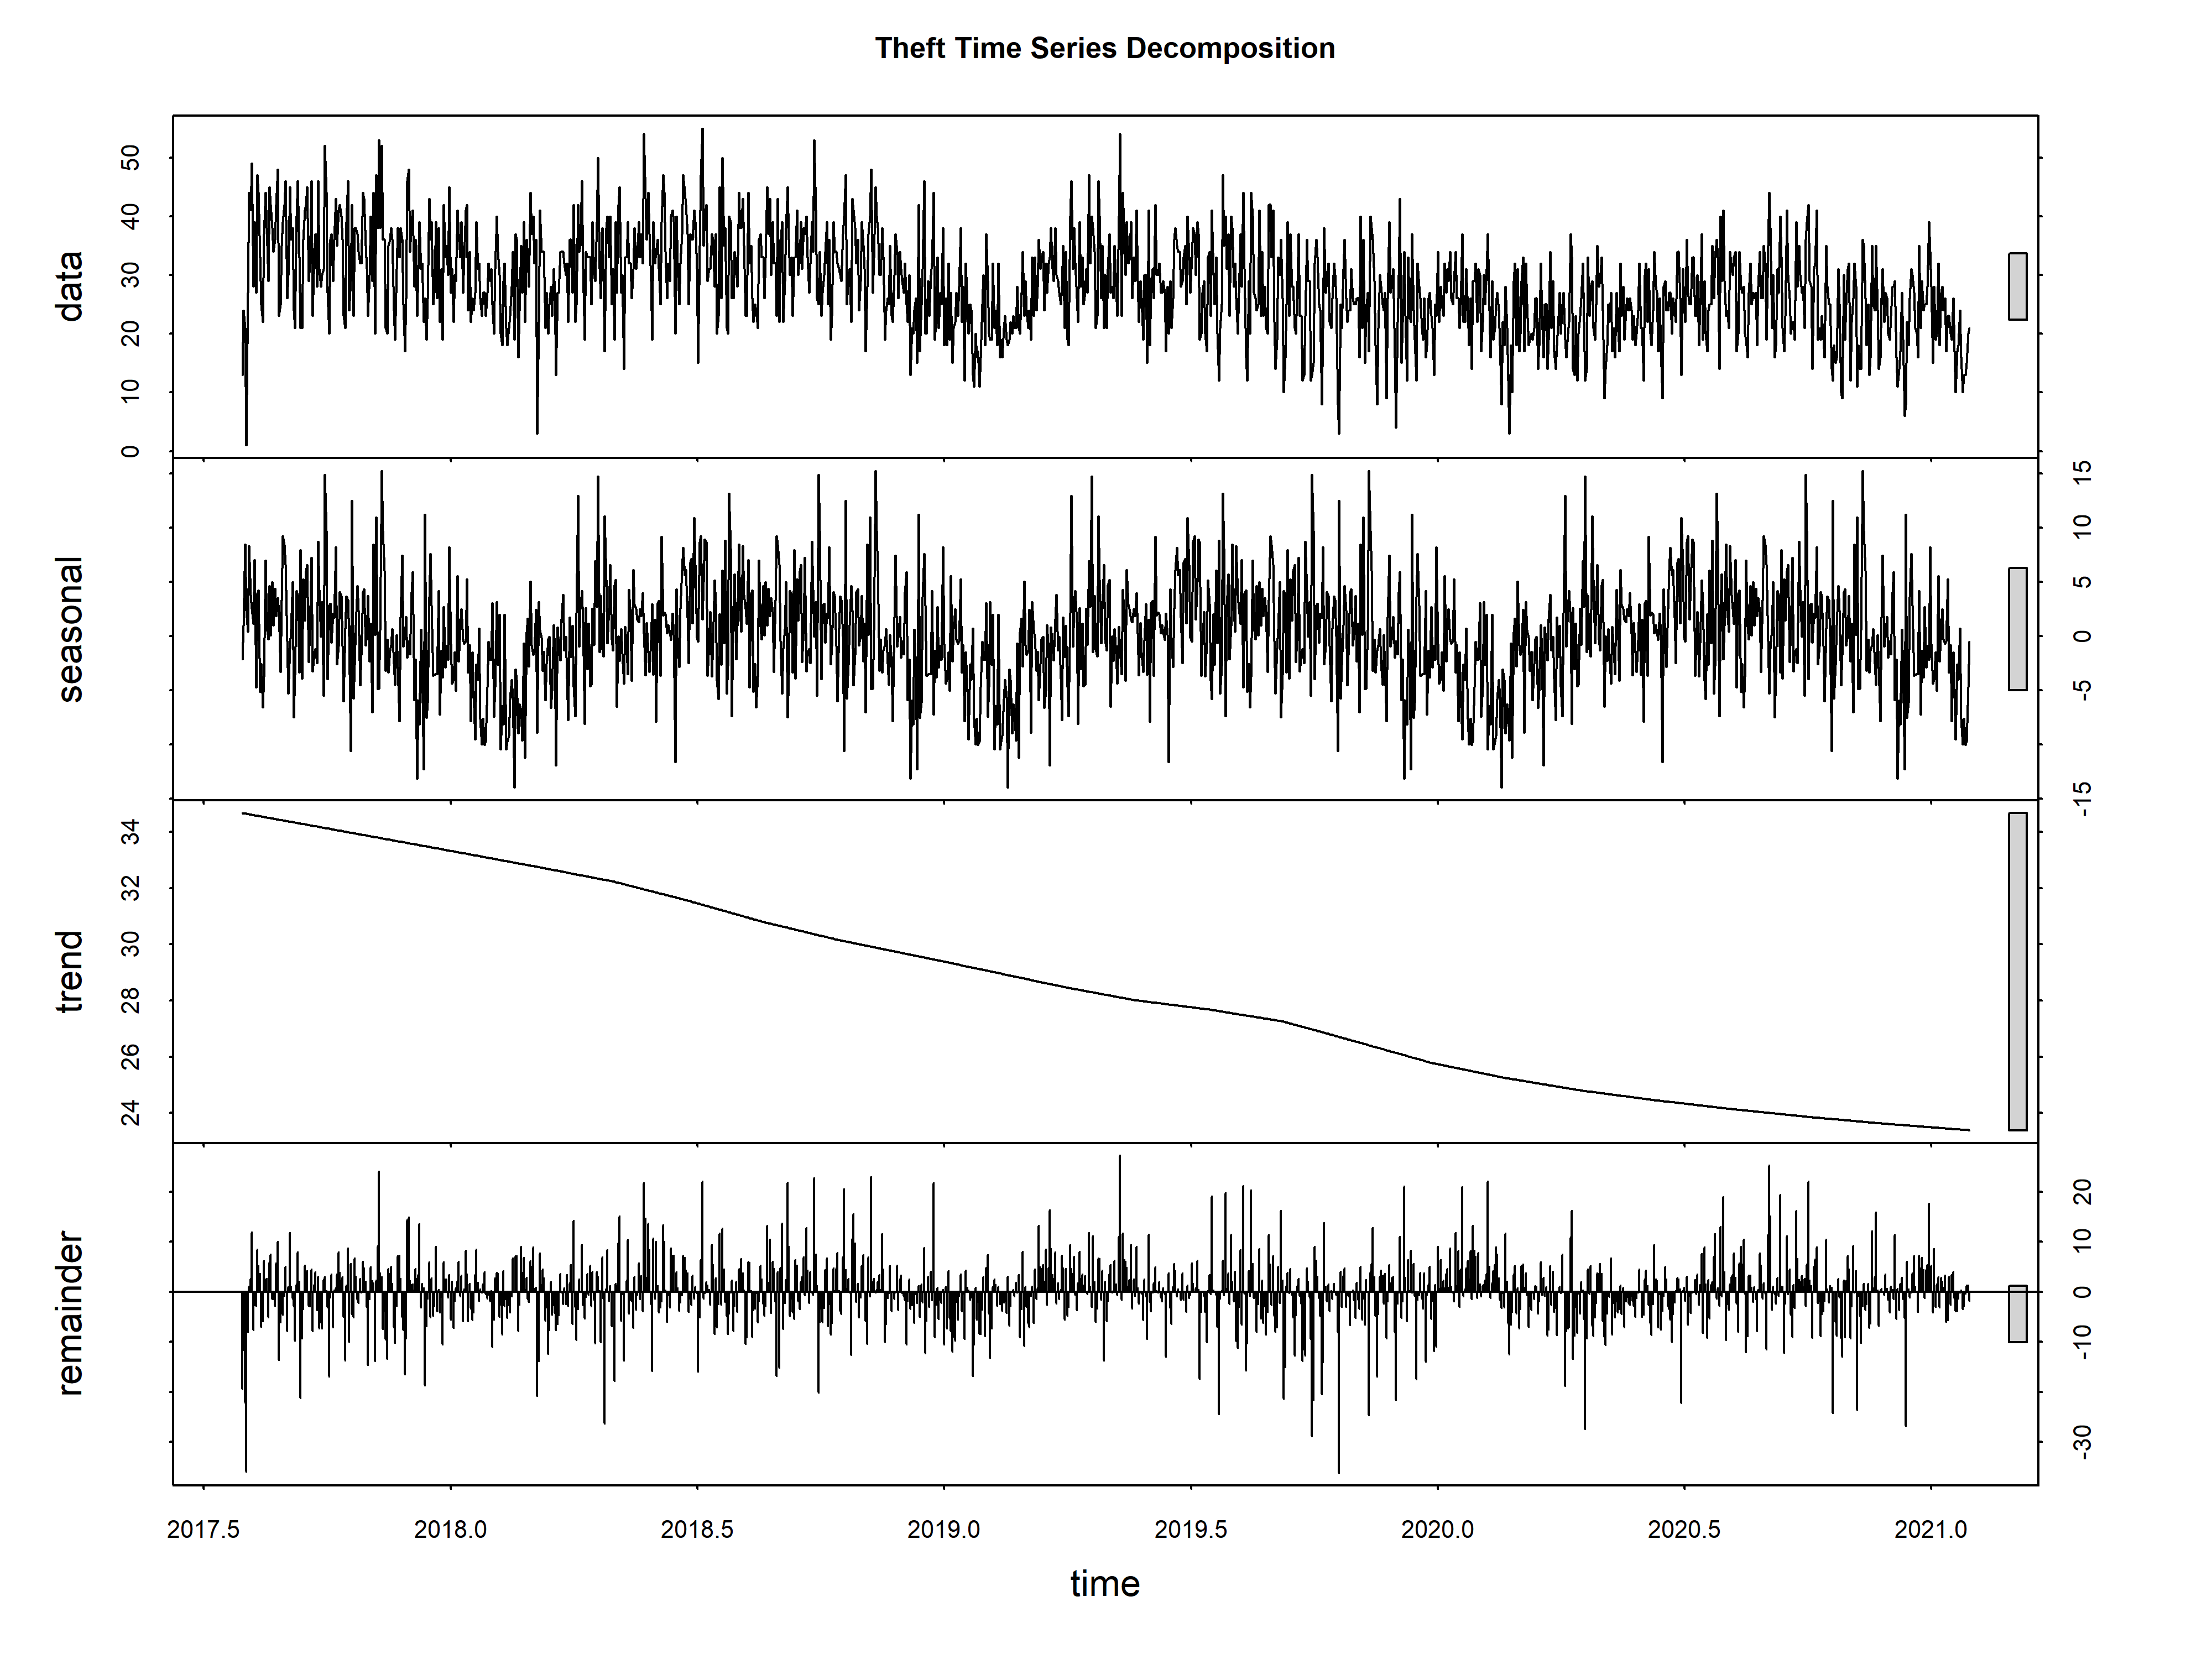
\includegraphics[width=\textwidth]{./figures/plot.theft_time_series_decomposition-1} \end{center}

\begin{center}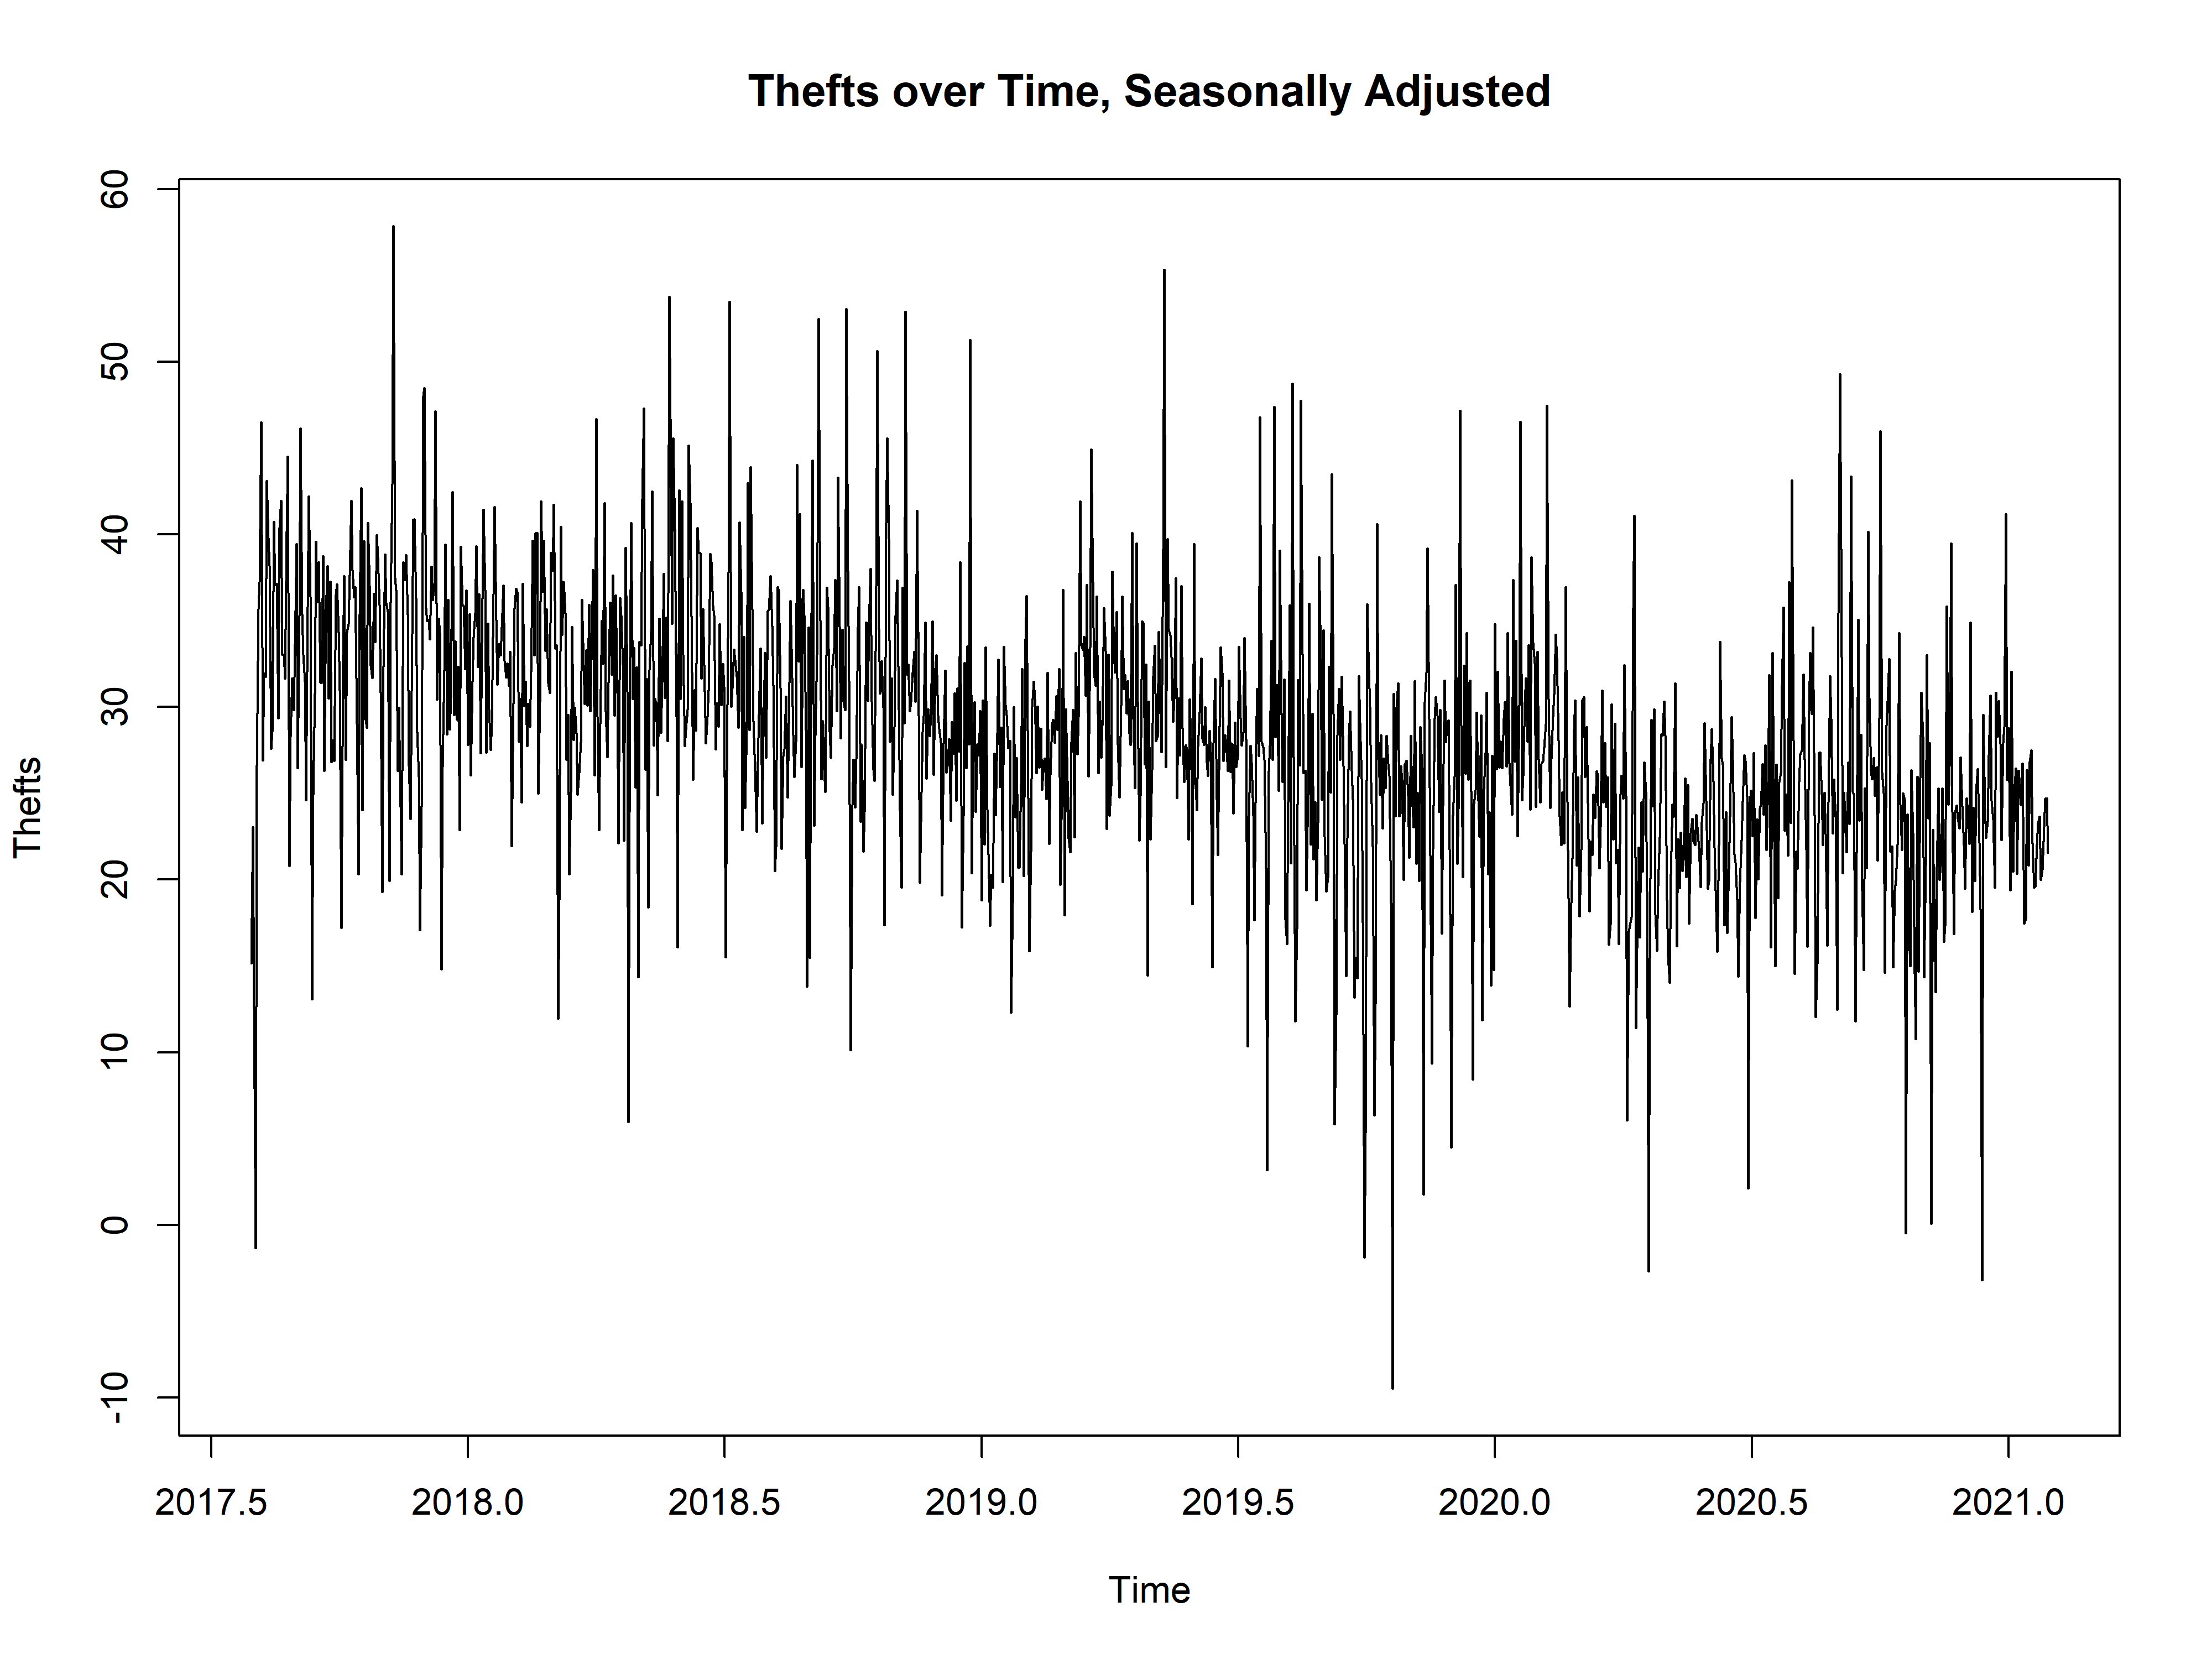
\includegraphics[width=\textwidth]{./figures/plot.theft_time_series_seasonal_adj-1} \end{center}

\hypertarget{robbery}{%
\subsection{Robbery}\label{robbery}}

\begin{center}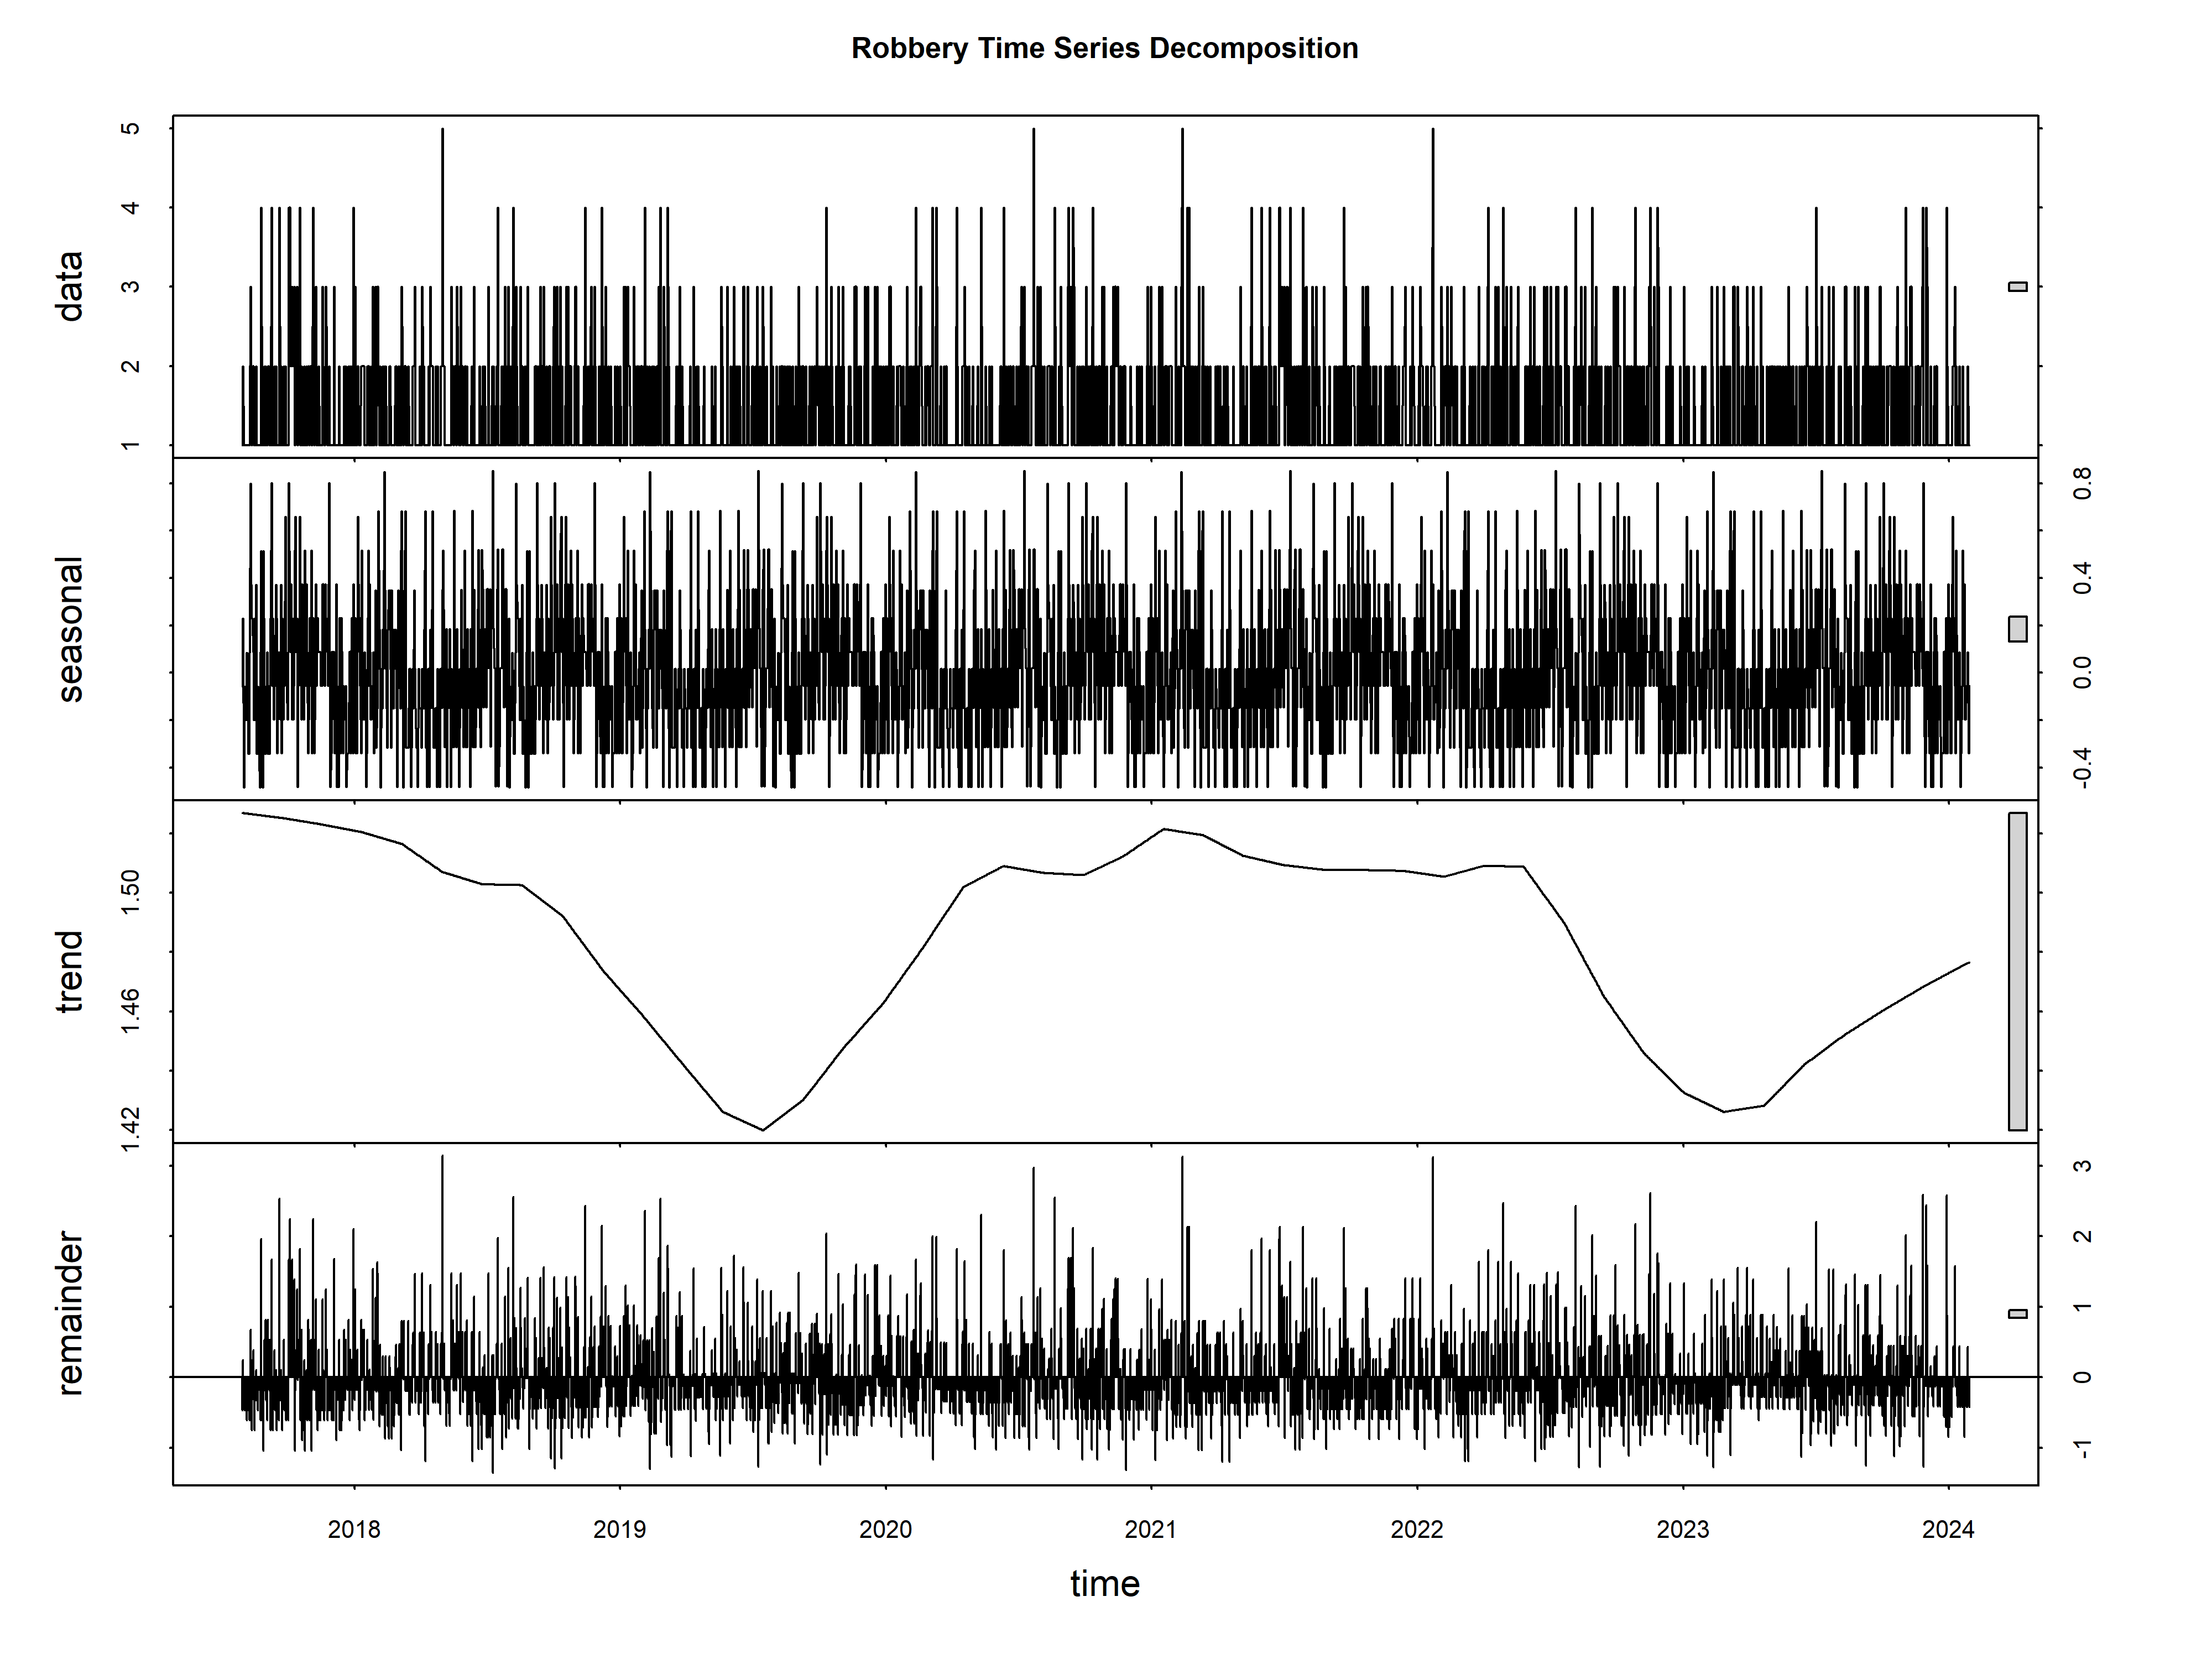
\includegraphics[width=\textwidth]{./figures/plot.robbery_time_series_decomposition-1} \end{center}

\hypertarget{motor-vehicle-theft}{%
\subsection{Motor Vehicle Theft}\label{motor-vehicle-theft}}

\begin{center}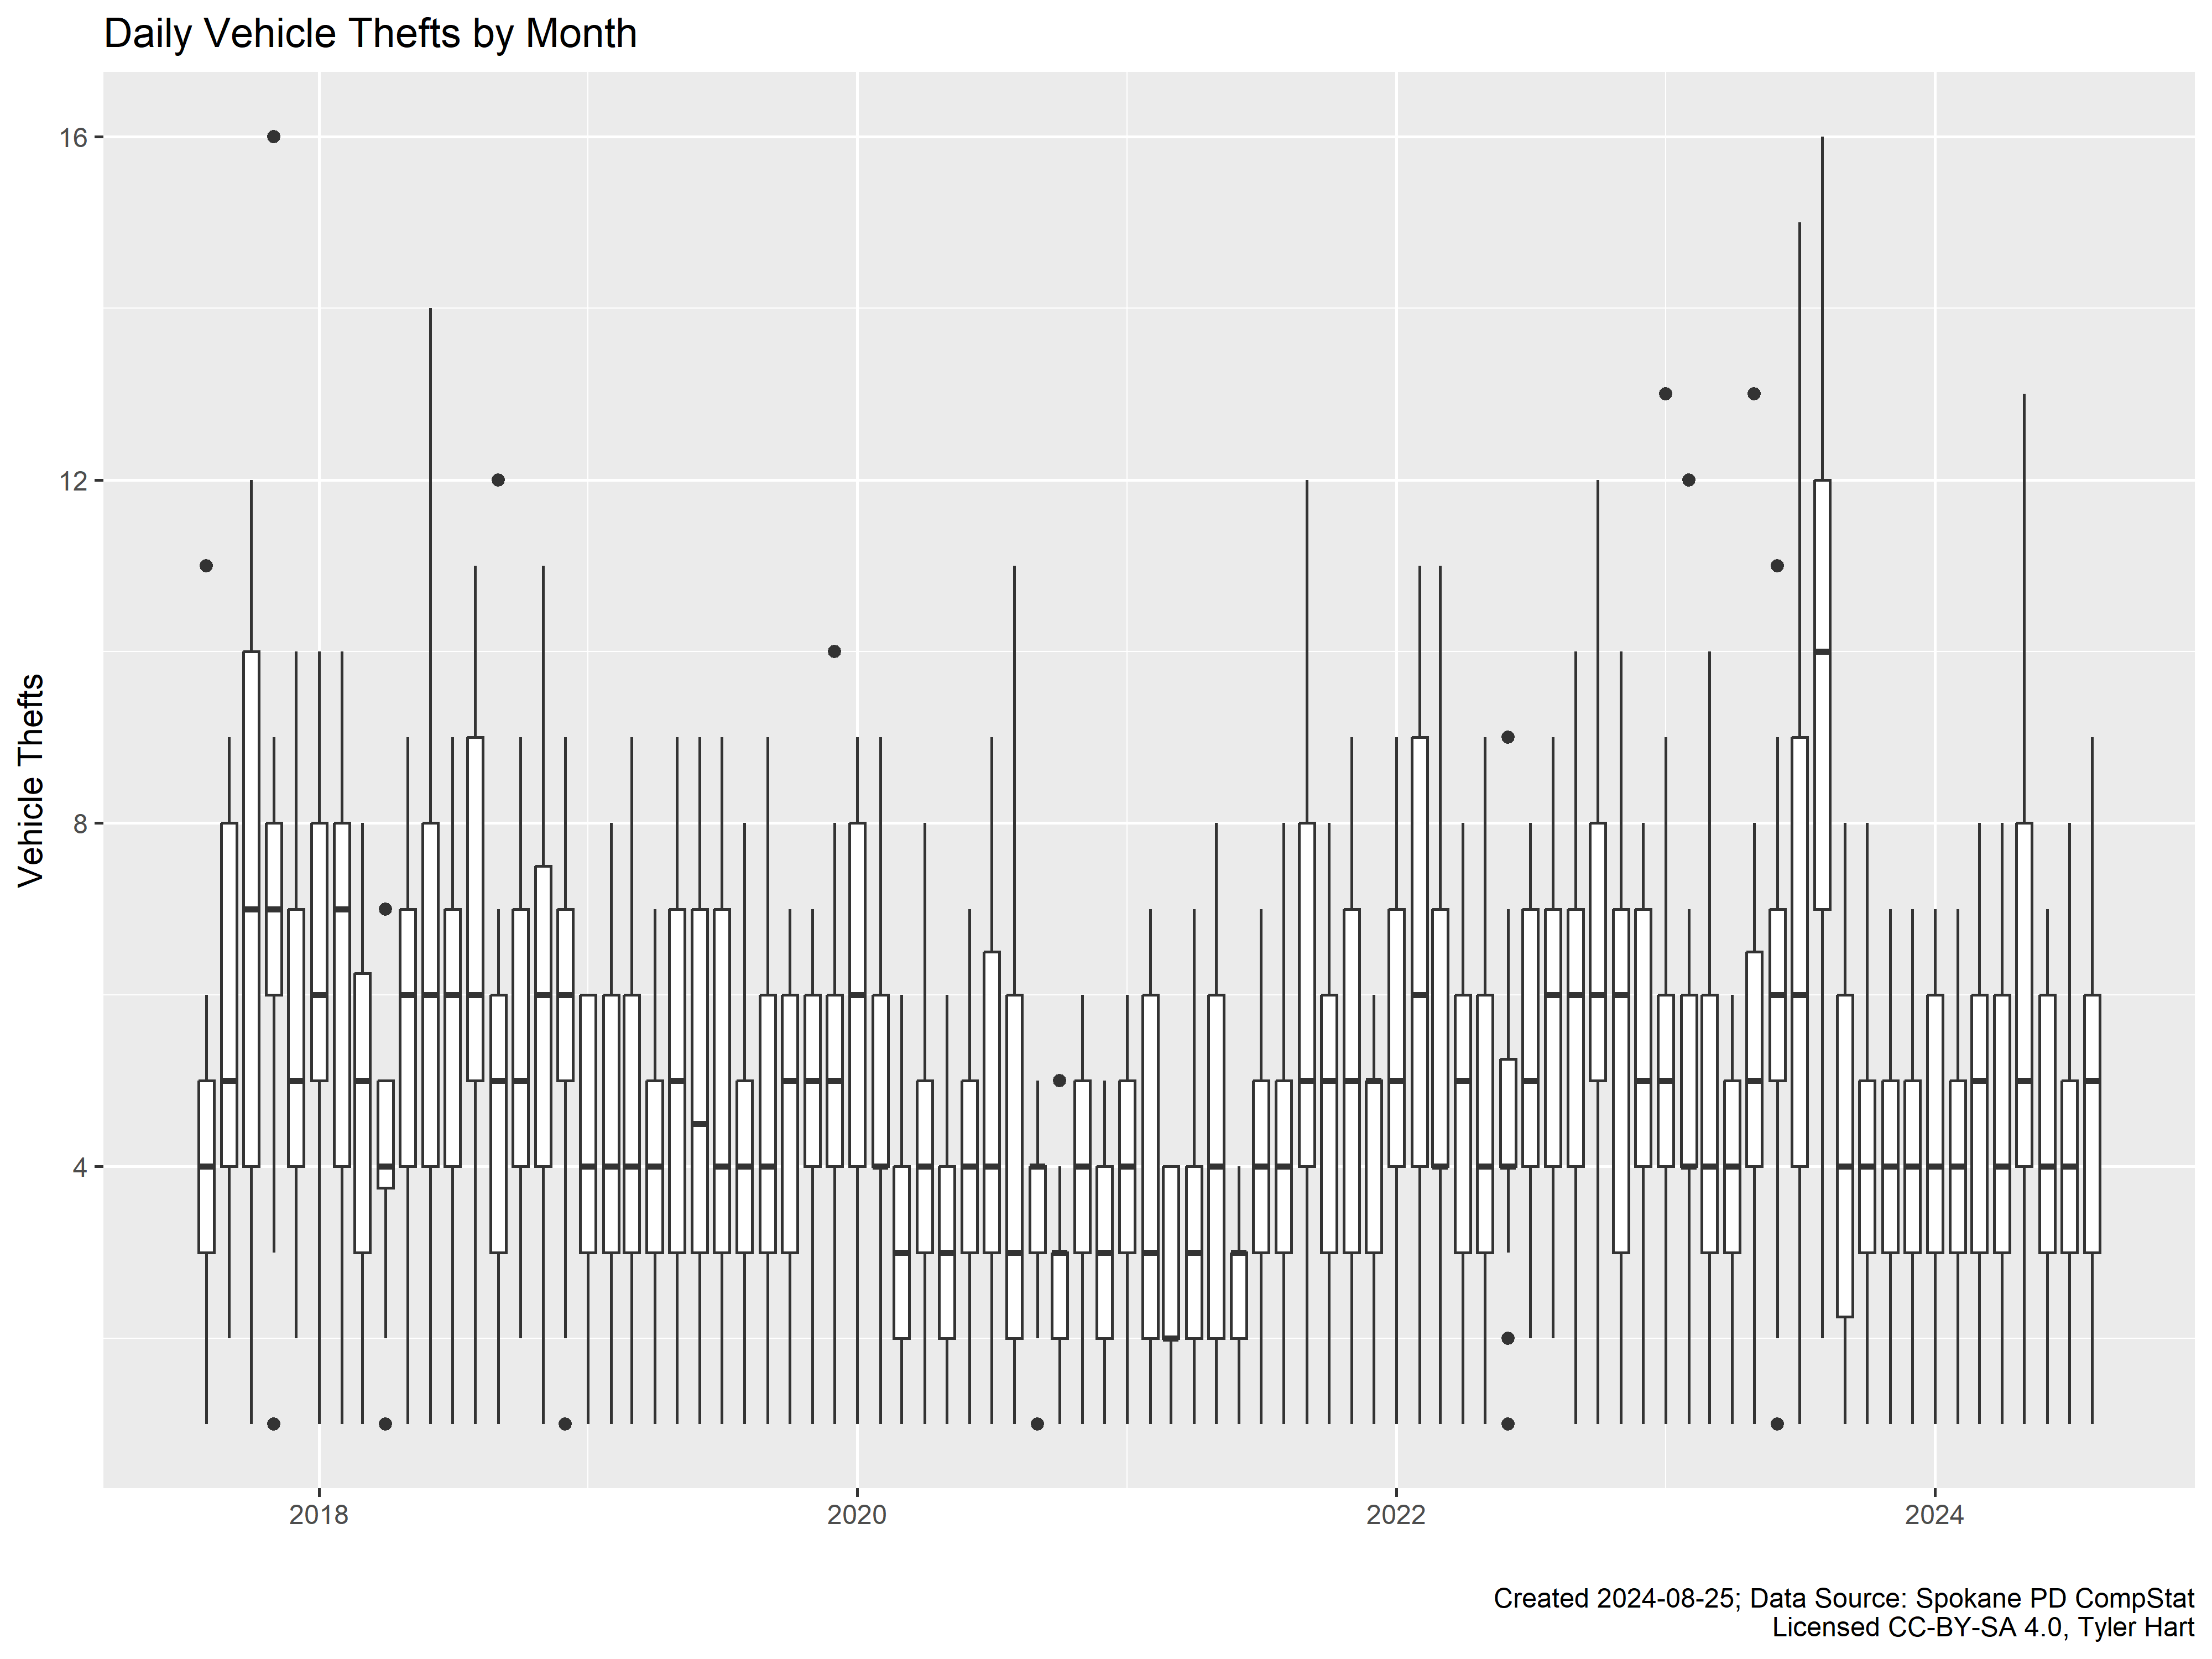
\includegraphics[width=\textwidth]{./figures/plot.boxplot_avg_daily_vehtheft_by_month-1} \end{center}

\begin{center}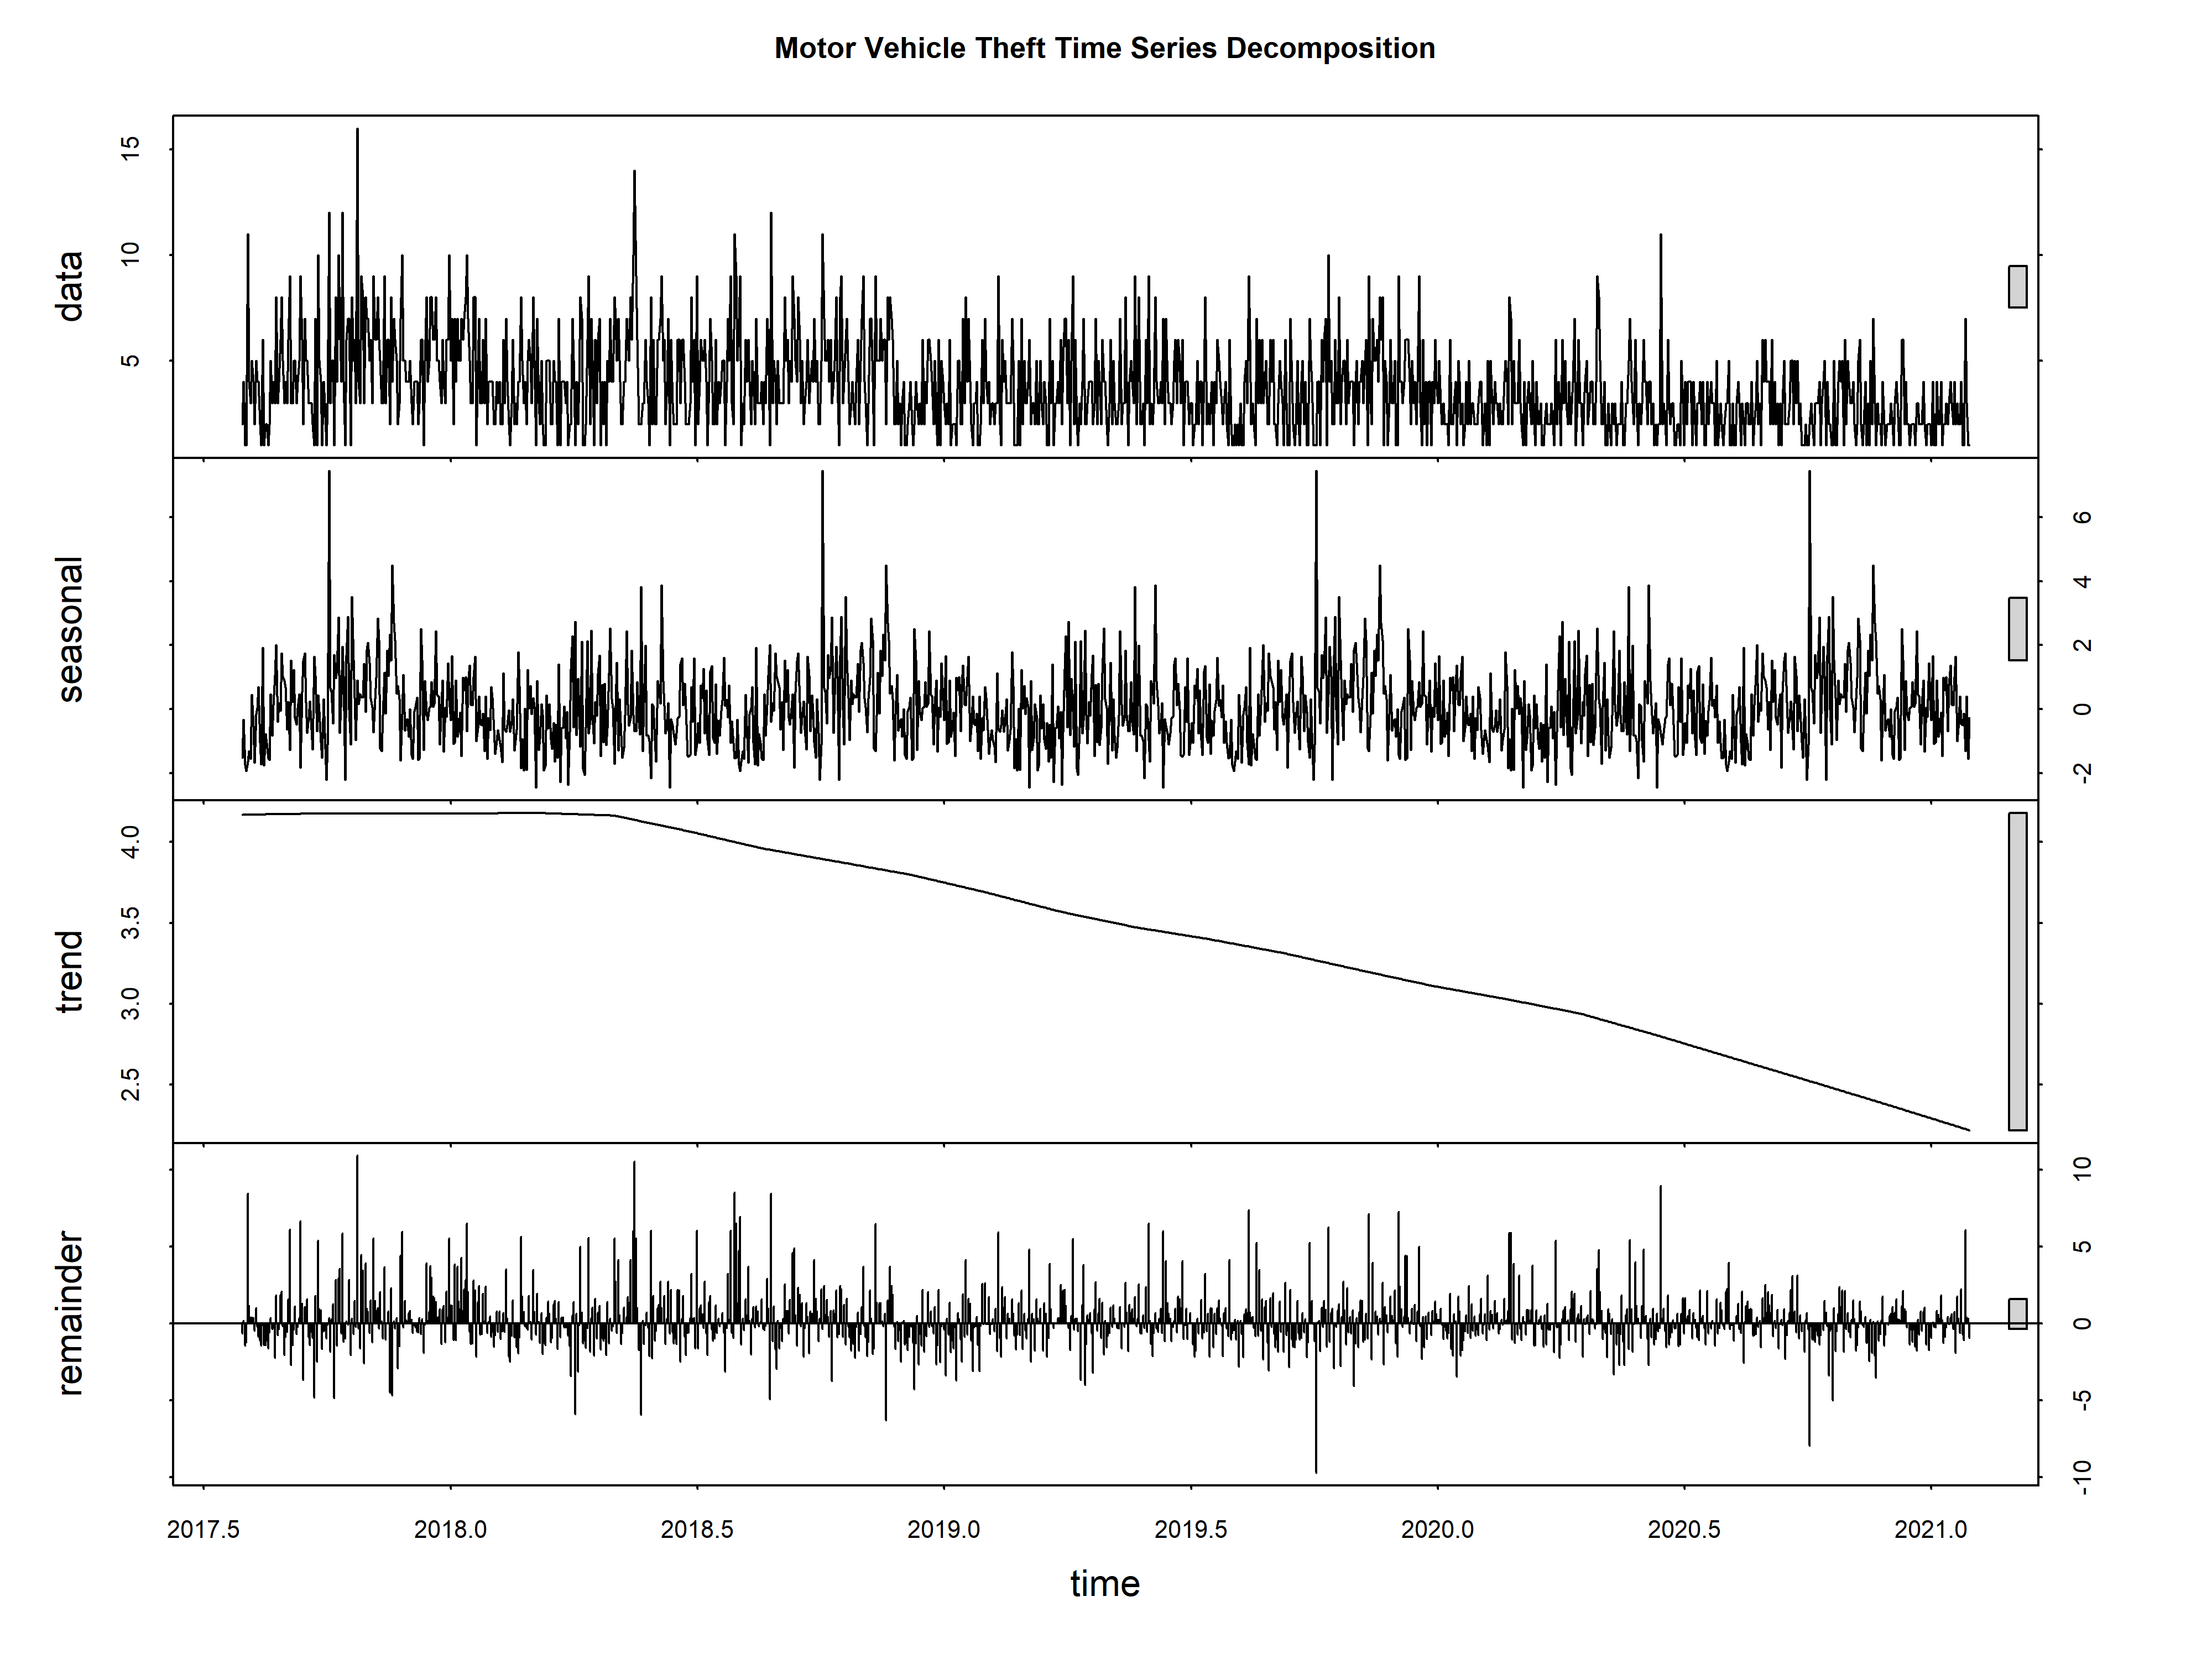
\includegraphics[width=\textwidth]{./figures/plot.veh_theft_time_series_decomposition-1} \end{center}

\begin{center}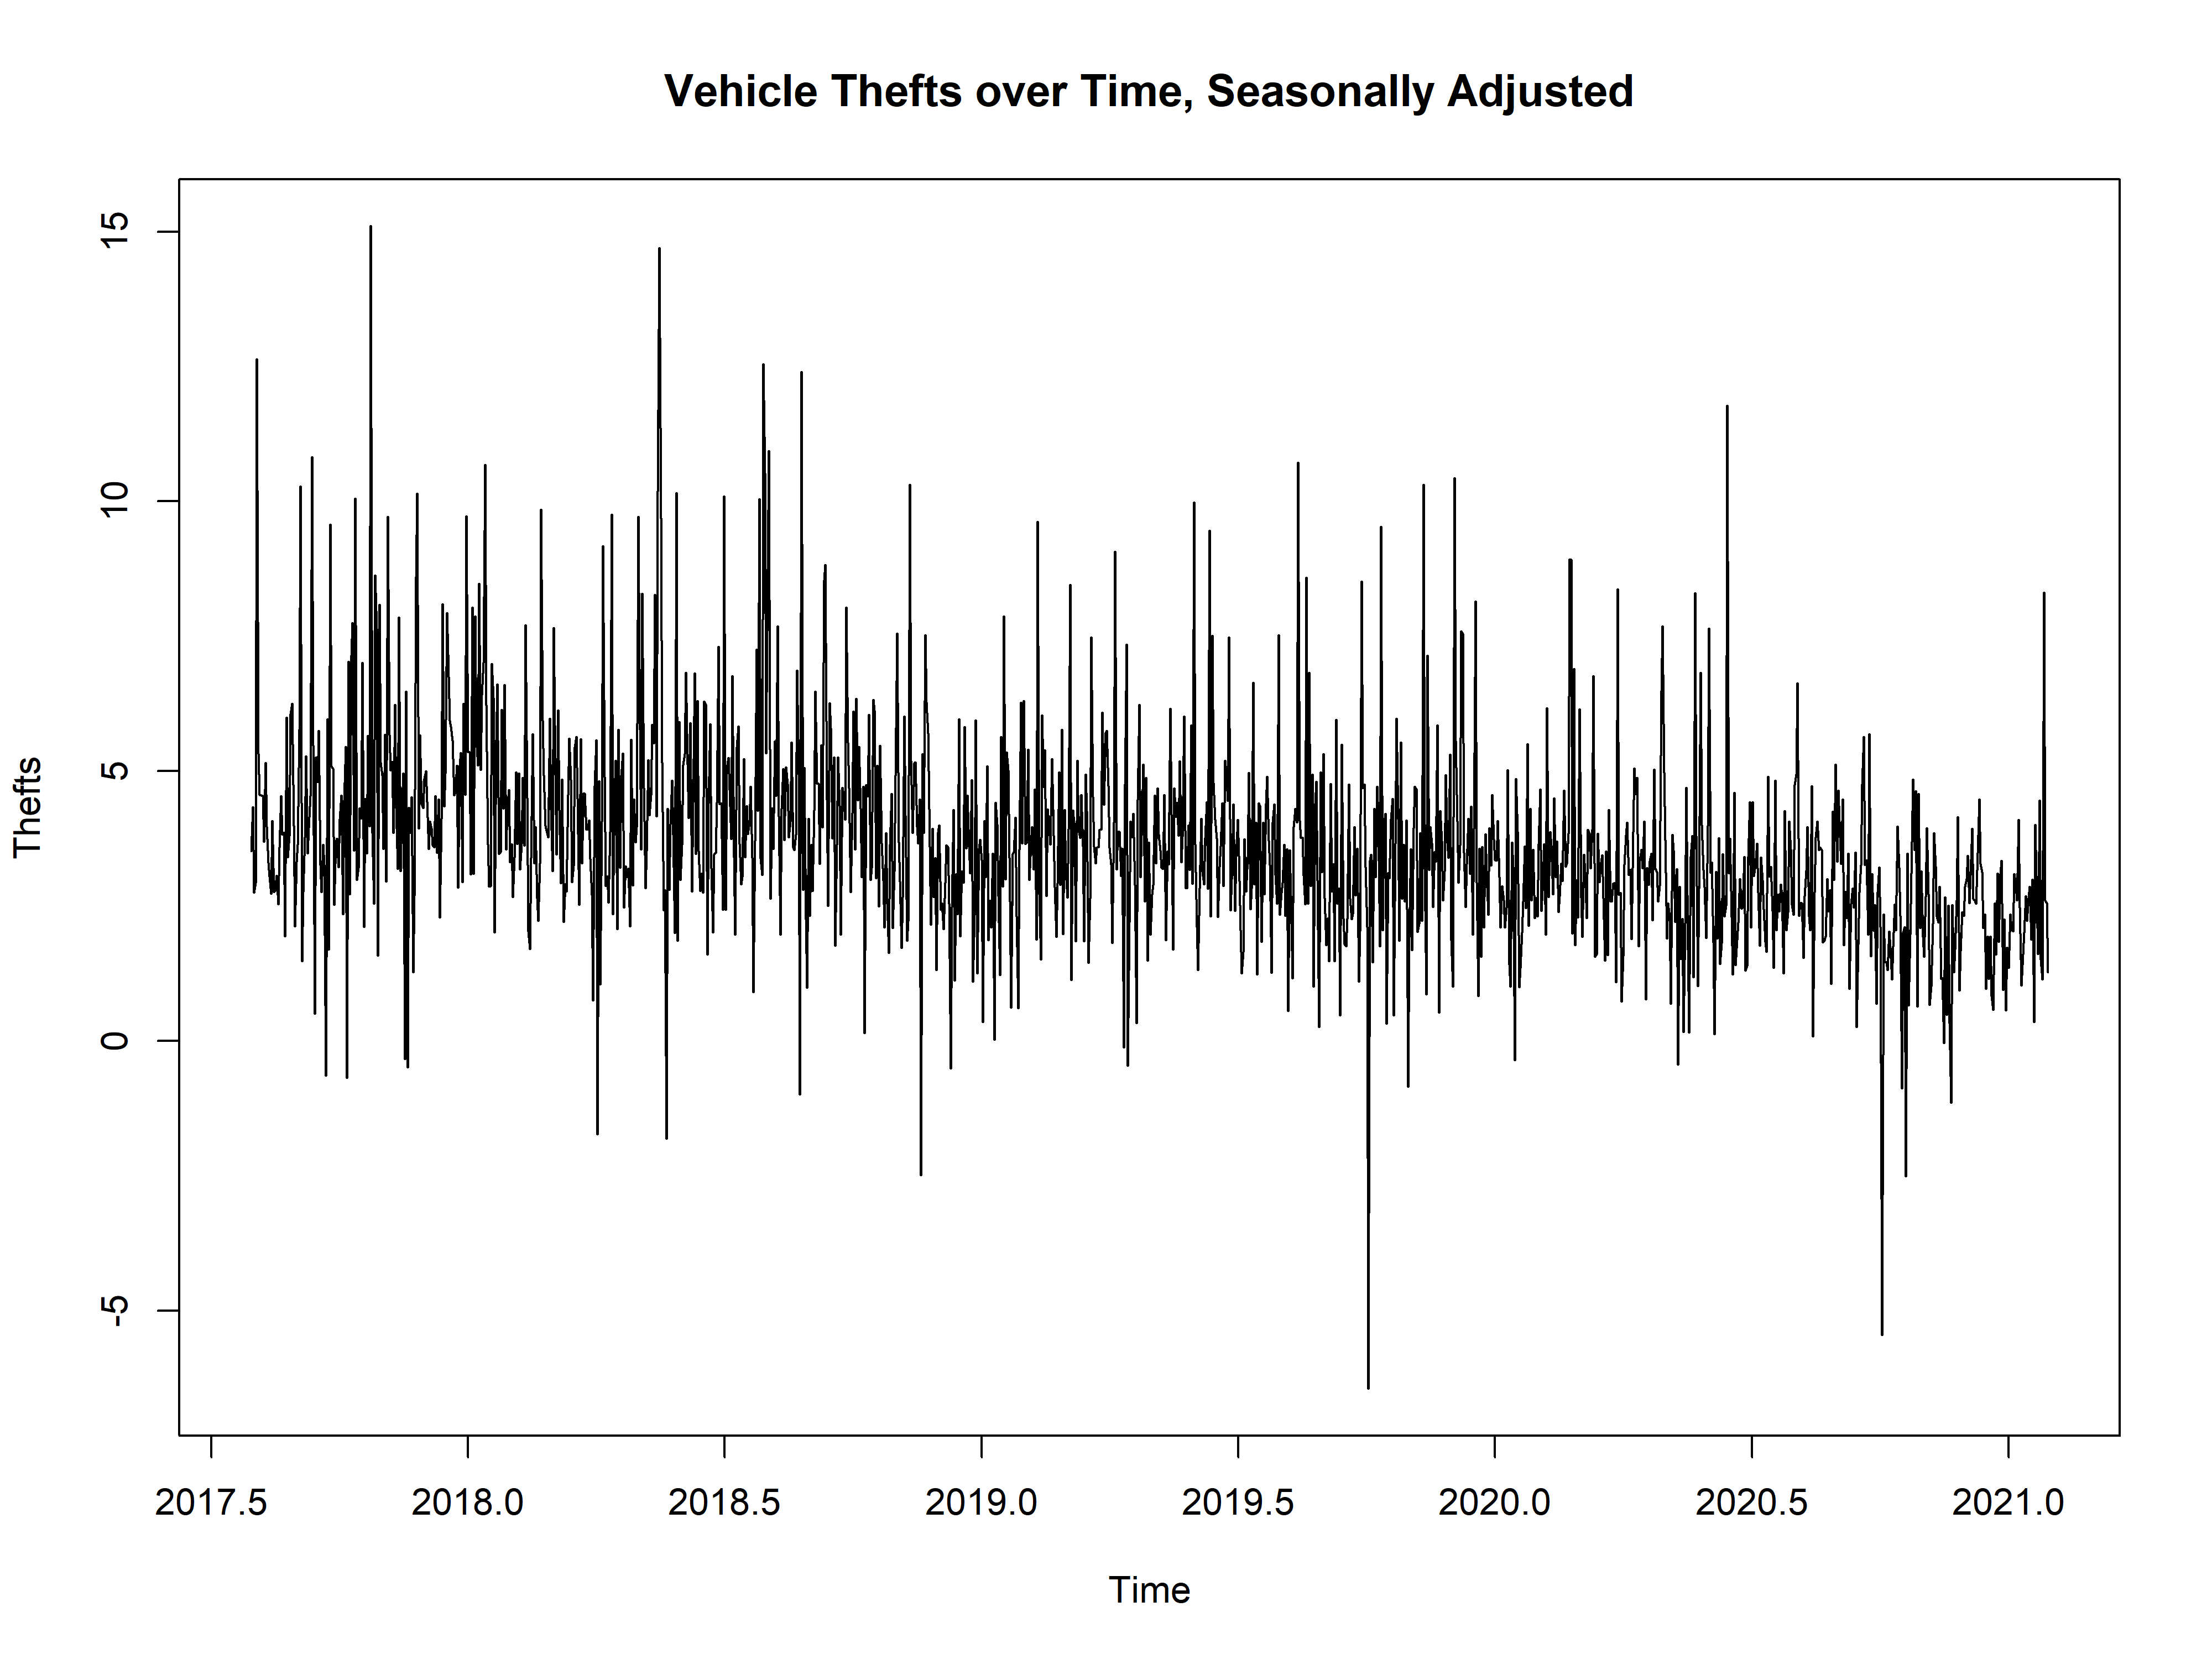
\includegraphics[width=\textwidth]{./figures/plot.veh_theft_time_series_seasonal_adj-1} \end{center}

\end{document}
